\documentclass[twoside]{book}

% Packages required by doxygen
\usepackage{calc}
\usepackage{doxygen}
\usepackage{graphicx}
\usepackage[utf8]{inputenc}
\usepackage{makeidx}
\usepackage{multicol}
\usepackage{multirow}
\usepackage{textcomp}
\usepackage[table]{xcolor}

% Font selection
\usepackage[T1]{fontenc}
\usepackage{mathptmx}
\usepackage[scaled=.90]{helvet}
\usepackage{courier}
\usepackage{amssymb}
\usepackage{sectsty}
\renewcommand{\familydefault}{\sfdefault}
\allsectionsfont{%
  \fontseries{bc}\selectfont%
  \color{darkgray}%
}
\renewcommand{\DoxyLabelFont}{%
  \fontseries{bc}\selectfont%
  \color{darkgray}%
}

% Page & text layout
\usepackage{geometry}
\geometry{%
  a4paper,%
  top=2.5cm,%
  bottom=2.5cm,%
  left=2.5cm,%
  right=2.5cm%
}
\tolerance=750
\hfuzz=15pt
\hbadness=750
\setlength{\emergencystretch}{15pt}
\setlength{\parindent}{0cm}
\setlength{\parskip}{0.2cm}
\makeatletter
\renewcommand{\paragraph}{%
  \@startsection{paragraph}{4}{0ex}{-1.0ex}{1.0ex}{%
    \normalfont\normalsize\bfseries\SS@parafont%
  }%
}
\renewcommand{\subparagraph}{%
  \@startsection{subparagraph}{5}{0ex}{-1.0ex}{1.0ex}{%
    \normalfont\normalsize\bfseries\SS@subparafont%
  }%
}
\makeatother

% Headers & footers
\usepackage{fancyhdr}
\pagestyle{fancyplain}
\fancyhead[LE]{\fancyplain{}{\bfseries\thepage}}
\fancyhead[CE]{\fancyplain{}{}}
\fancyhead[RE]{\fancyplain{}{\bfseries\leftmark}}
\fancyhead[LO]{\fancyplain{}{\bfseries\rightmark}}
\fancyhead[CO]{\fancyplain{}{}}
\fancyhead[RO]{\fancyplain{}{\bfseries\thepage}}
\fancyfoot[LE]{\fancyplain{}{}}
\fancyfoot[CE]{\fancyplain{}{}}
\fancyfoot[RE]{\fancyplain{}{\bfseries\scriptsize Generated on Tue Sep 15 2015 17\-:35\-:10 for Fun\-G by Doxygen }}
\fancyfoot[LO]{\fancyplain{}{\bfseries\scriptsize Generated on Tue Sep 15 2015 17\-:35\-:10 for Fun\-G by Doxygen }}
\fancyfoot[CO]{\fancyplain{}{}}
\fancyfoot[RO]{\fancyplain{}{}}
\renewcommand{\footrulewidth}{0.4pt}
\renewcommand{\chaptermark}[1]{%
  \markboth{#1}{}%
}
\renewcommand{\sectionmark}[1]{%
  \markright{\thesection\ #1}%
}

% Indices & bibliography
\usepackage{natbib}
\usepackage[titles]{tocloft}
\setcounter{tocdepth}{3}
\setcounter{secnumdepth}{5}
\makeindex

% Hyperlinks (required, but should be loaded last)
\usepackage{ifpdf}
\ifpdf
  \usepackage[pdftex,pagebackref=true]{hyperref}
\else
  \usepackage[ps2pdf,pagebackref=true]{hyperref}
\fi
\hypersetup{%
  colorlinks=true,%
  linkcolor=blue,%
  citecolor=blue,%
  unicode%
}

% Custom commands
\newcommand{\clearemptydoublepage}{%
  \newpage{\pagestyle{empty}\cleardoublepage}%
}


%===== C O N T E N T S =====

\begin{document}

% Titlepage & ToC
\hypersetup{pageanchor=false}
\pagenumbering{roman}
\begin{titlepage}
\vspace*{7cm}
\begin{center}%
{\Large Fun\-G }\\
\vspace*{1cm}
{\large Generated by Doxygen 1.8.6}\\
\vspace*{0.5cm}
{\small Tue Sep 15 2015 17:35:10}\\
\end{center}
\end{titlepage}
\clearemptydoublepage
\tableofcontents
\clearemptydoublepage
\pagenumbering{arabic}
\hypersetup{pageanchor=true}

%--- Begin generated contents ---
\chapter{Fun\-G documentation}
\label{index}\hypertarget{index}{}\input{index}
\chapter{Module Index}
\input{modules}
\chapter{Namespace Index}
\section{Namespace List}
Here is a list of all documented namespaces with brief descriptions\-:\begin{DoxyCompactList}
\item\contentsline{section}{\hyperlink{namespaceChecks}{Checks} \\*Static checks for the presence of different operators and functions }{\pageref{namespaceChecks}}{}
\item\contentsline{section}{\hyperlink{namespaceCMath}{C\-Math} \\*Wrappers for functions from $<$cmath$>$ }{\pageref{namespaceCMath}}{}
\item\contentsline{section}{\hyperlink{namespaceLinearAlgebra}{Linear\-Algebra} \\*Functionality from linear algebra such as (modified) principal and mixed matrix invariants }{\pageref{namespaceLinearAlgebra}}{}
\item\contentsline{section}{\hyperlink{namespaceMathematicalOperations}{Mathematical\-Operations} \\*Mathematical operations and corresponding differentation rules }{\pageref{namespaceMathematicalOperations}}{}
\item\contentsline{section}{\hyperlink{namespaceRFFGen}{R\-F\-F\-Gen} \\*Main namespace of the \hyperlink{namespaceRFFGen}{R\-F\-F\-Gen} library }{\pageref{namespaceRFFGen}}{}
\end{DoxyCompactList}

\chapter{Hierarchical Index}
\section{Class Hierarchy}
This inheritance list is sorted roughly, but not completely, alphabetically\-:\begin{DoxyCompactList}
\item \contentsline{section}{R\-F\-F\-Gen\-:\-:Base}{\pageref{structRFFGen_1_1Base}}{}
\begin{DoxyCompactList}
\item \contentsline{section}{R\-F\-F\-Gen\-:\-:Constant$<$ Matrix $>$}{\pageref{structRFFGen_1_1Constant}}{}
\item \contentsline{section}{R\-F\-F\-Gen\-:\-:Identity$<$ Matrix $>$}{\pageref{structRFFGen_1_1Identity}}{}
\item \contentsline{section}{R\-F\-F\-Gen\-:\-:Linear\-Algebra\-:\-:Linearized\-Strain\-Tensor$<$ Matrix $>$}{\pageref{classRFFGen_1_1LinearAlgebra_1_1LinearizedStrainTensor}}{}
\item \contentsline{section}{R\-F\-F\-Gen\-:\-:Mathematical\-Operations\-:\-:Product$<$ Trace$<$ Matrix $>$, Constant$<$ Matrix $>$ $>$}{\pageref{structRFFGen_1_1MathematicalOperations_1_1Product}}{}
\item \contentsline{section}{R\-F\-F\-Gen\-:\-:C\-Math\-:\-:A\-Sin}{\pageref{structRFFGen_1_1CMath_1_1ASin}}{}
\item \contentsline{section}{R\-F\-F\-Gen\-:\-:C\-Math\-:\-:Cos}{\pageref{structRFFGen_1_1CMath_1_1Cos}}{}
\item \contentsline{section}{R\-F\-F\-Gen\-:\-:C\-Math\-:\-:Exp}{\pageref{structRFFGen_1_1CMath_1_1Exp}}{}
\item \contentsline{section}{R\-F\-F\-Gen\-:\-:C\-Math\-:\-:Exp2}{\pageref{structRFFGen_1_1CMath_1_1Exp2}}{}
\item \contentsline{section}{R\-F\-F\-Gen\-:\-:C\-Math\-:\-:L\-N}{\pageref{structRFFGen_1_1CMath_1_1LN}}{}
\item \contentsline{section}{R\-F\-F\-Gen\-:\-:C\-Math\-:\-:Log10}{\pageref{structRFFGen_1_1CMath_1_1Log10}}{}
\item \contentsline{section}{R\-F\-F\-Gen\-:\-:C\-Math\-:\-:Log2}{\pageref{structRFFGen_1_1CMath_1_1Log2}}{}
\item \contentsline{section}{R\-F\-F\-Gen\-:\-:C\-Math\-:\-:Pow$<$ dividend, divisor $>$}{\pageref{structRFFGen_1_1CMath_1_1Pow}}{}
\item \contentsline{section}{R\-F\-F\-Gen\-:\-:C\-Math\-:\-:Sin}{\pageref{structRFFGen_1_1CMath_1_1Sin}}{}
\item \contentsline{section}{R\-F\-F\-Gen\-:\-:C\-Math\-:\-:Tan}{\pageref{structRFFGen_1_1CMath_1_1Tan}}{}
\item \contentsline{section}{R\-F\-F\-Gen\-:\-:Concepts\-:\-:Function\-Concept}{\pageref{structRFFGen_1_1Concepts_1_1FunctionConcept}}{}
\item \contentsline{section}{R\-F\-F\-Gen\-:\-:Constant$<$ Type, class $>$}{\pageref{structRFFGen_1_1Constant}}{}
\item \contentsline{section}{R\-F\-F\-Gen\-:\-:Identity$<$ Arg, class $>$}{\pageref{structRFFGen_1_1Identity}}{}
\item \contentsline{section}{R\-F\-F\-Gen\-:\-:Linear\-Algebra\-:\-:Left\-Cauchy\-Green\-Strain\-Tensor$<$ Matrix, class $>$}{\pageref{classRFFGen_1_1LinearAlgebra_1_1LeftCauchyGreenStrainTensor}}{}
\item \contentsline{section}{R\-F\-F\-Gen\-:\-:Linear\-Algebra\-:\-:Linearized\-Strain\-Tensor$<$ Matrix, class $>$}{\pageref{classRFFGen_1_1LinearAlgebra_1_1LinearizedStrainTensor}}{}
\item \contentsline{section}{R\-F\-F\-Gen\-:\-:Linear\-Algebra\-:\-:Second\-Principal\-Invariant$<$ Matrix, class $>$}{\pageref{classRFFGen_1_1LinearAlgebra_1_1SecondPrincipalInvariant}}{}
\item \contentsline{section}{R\-F\-F\-Gen\-:\-:Linear\-Algebra\-:\-:Shifted\-Invariant$<$ Invariant, offset $>$}{\pageref{classRFFGen_1_1LinearAlgebra_1_1ShiftedInvariant}}{}
\item \contentsline{section}{R\-F\-F\-Gen\-:\-:Linear\-Algebra\-:\-:Squared\-Euclidean\-Norm$<$ Matrix, class $>$}{\pageref{structRFFGen_1_1LinearAlgebra_1_1SquaredEuclideanNorm}}{}
\item \contentsline{section}{R\-F\-F\-Gen\-:\-:Linear\-Algebra\-:\-:Squared\-Matrix\-Norm$<$ Matrix, class $>$}{\pageref{structRFFGen_1_1LinearAlgebra_1_1SquaredMatrixNorm}}{}
\item \contentsline{section}{R\-F\-F\-Gen\-:\-:Mathematical\-Operations\-:\-:Chain$<$ F, G, class, class $>$}{\pageref{structRFFGen_1_1MathematicalOperations_1_1Chain}}{}
\item \contentsline{section}{R\-F\-F\-Gen\-:\-:Mathematical\-Operations\-:\-:Product$<$ F, G, class, class $>$}{\pageref{structRFFGen_1_1MathematicalOperations_1_1Product}}{}
\item \contentsline{section}{R\-F\-F\-Gen\-:\-:Mathematical\-Operations\-:\-:Scale$<$ F, class $>$}{\pageref{structRFFGen_1_1MathematicalOperations_1_1Scale}}{}
\item \contentsline{section}{R\-F\-F\-Gen\-:\-:Mathematical\-Operations\-:\-:Squared$<$ F, class $>$}{\pageref{structRFFGen_1_1MathematicalOperations_1_1Squared}}{}
\item \contentsline{section}{R\-F\-F\-Gen\-:\-:Mathematical\-Operations\-:\-:Sum$<$ F, G, Check\-F, Check\-G $>$}{\pageref{structRFFGen_1_1MathematicalOperations_1_1Sum}}{}
\item \contentsline{section}{R\-F\-F\-Gen\-:\-:Variable$<$ T, id $>$}{\pageref{structRFFGen_1_1Variable}}{}
\item \contentsline{section}{R\-F\-F\-Gen\-:\-:Mathematical\-Operations\-:\-:Sum$<$ Identity$<$ Matrix $>$, Mathematical\-Operations\-:\-:Product$<$ Trace$<$ Matrix $>$, Constant$<$ Matrix $>$ $>$ $>$}{\pageref{structRFFGen_1_1MathematicalOperations_1_1Sum}}{}
\begin{DoxyCompactList}
\item \contentsline{section}{R\-F\-F\-Gen\-:\-:Linear\-Algebra\-:\-:Deviator$<$ Matrix, class $>$}{\pageref{structRFFGen_1_1LinearAlgebra_1_1Deviator}}{}
\end{DoxyCompactList}
\item \contentsline{section}{R\-F\-F\-Gen\-:\-:Mathematical\-Operations\-:\-:Sum$<$ Linearized\-Strain\-Tensor$<$ Matrix $>$, Geometric\-Nonlinearity$<$ Matrix $>$ $>$}{\pageref{structRFFGen_1_1MathematicalOperations_1_1Sum}}{}
\begin{DoxyCompactList}
\item \contentsline{section}{R\-F\-F\-Gen\-:\-:Linear\-Algebra\-:\-:Strain\-Tensor$<$ Matrix $>$}{\pageref{classRFFGen_1_1LinearAlgebra_1_1StrainTensor}}{}
\end{DoxyCompactList}
\end{DoxyCompactList}
\item Chainer\begin{DoxyCompactList}
\item \contentsline{section}{R\-F\-F\-Gen\-:\-:Mathematical\-Operations\-:\-:Product$<$ Trace$<$ Matrix $>$, Constant$<$ Matrix $>$ $>$}{\pageref{structRFFGen_1_1MathematicalOperations_1_1Product}}{}
\item \contentsline{section}{R\-F\-F\-Gen\-:\-:C\-Math\-:\-:A\-Sin}{\pageref{structRFFGen_1_1CMath_1_1ASin}}{}
\item \contentsline{section}{R\-F\-F\-Gen\-:\-:C\-Math\-:\-:Cos}{\pageref{structRFFGen_1_1CMath_1_1Cos}}{}
\item \contentsline{section}{R\-F\-F\-Gen\-:\-:C\-Math\-:\-:Exp}{\pageref{structRFFGen_1_1CMath_1_1Exp}}{}
\item \contentsline{section}{R\-F\-F\-Gen\-:\-:C\-Math\-:\-:Exp2}{\pageref{structRFFGen_1_1CMath_1_1Exp2}}{}
\item \contentsline{section}{R\-F\-F\-Gen\-:\-:C\-Math\-:\-:L\-N}{\pageref{structRFFGen_1_1CMath_1_1LN}}{}
\item \contentsline{section}{R\-F\-F\-Gen\-:\-:C\-Math\-:\-:Log10}{\pageref{structRFFGen_1_1CMath_1_1Log10}}{}
\item \contentsline{section}{R\-F\-F\-Gen\-:\-:C\-Math\-:\-:Log2}{\pageref{structRFFGen_1_1CMath_1_1Log2}}{}
\item \contentsline{section}{R\-F\-F\-Gen\-:\-:C\-Math\-:\-:Pow$<$ dividend, divisor $>$}{\pageref{structRFFGen_1_1CMath_1_1Pow}}{}
\item \contentsline{section}{R\-F\-F\-Gen\-:\-:C\-Math\-:\-:Sin}{\pageref{structRFFGen_1_1CMath_1_1Sin}}{}
\item \contentsline{section}{R\-F\-F\-Gen\-:\-:C\-Math\-:\-:Tan}{\pageref{structRFFGen_1_1CMath_1_1Tan}}{}
\item \contentsline{section}{R\-F\-F\-Gen\-:\-:Mathematical\-Operations\-:\-:Chain$<$ F, G, class, class $>$}{\pageref{structRFFGen_1_1MathematicalOperations_1_1Chain}}{}
\item \contentsline{section}{R\-F\-F\-Gen\-:\-:Mathematical\-Operations\-:\-:Product$<$ F, G, class, class $>$}{\pageref{structRFFGen_1_1MathematicalOperations_1_1Product}}{}
\item \contentsline{section}{R\-F\-F\-Gen\-:\-:Mathematical\-Operations\-:\-:Scale$<$ F, class $>$}{\pageref{structRFFGen_1_1MathematicalOperations_1_1Scale}}{}
\item \contentsline{section}{R\-F\-F\-Gen\-:\-:Mathematical\-Operations\-:\-:Squared$<$ F, class $>$}{\pageref{structRFFGen_1_1MathematicalOperations_1_1Squared}}{}
\item \contentsline{section}{R\-F\-F\-Gen\-:\-:Mathematical\-Operations\-:\-:Sum$<$ F, G, Check\-F, Check\-G $>$}{\pageref{structRFFGen_1_1MathematicalOperations_1_1Sum}}{}
\item \contentsline{section}{R\-F\-F\-Gen\-:\-:Mathematical\-Operations\-:\-:Sum$<$ Identity$<$ Matrix $>$, Mathematical\-Operations\-:\-:Product$<$ Trace$<$ Matrix $>$, Constant$<$ Matrix $>$ $>$ $>$}{\pageref{structRFFGen_1_1MathematicalOperations_1_1Sum}}{}
\item \contentsline{section}{R\-F\-F\-Gen\-:\-:Mathematical\-Operations\-:\-:Sum$<$ Linearized\-Strain\-Tensor$<$ Matrix $>$, Geometric\-Nonlinearity$<$ Matrix $>$ $>$}{\pageref{structRFFGen_1_1MathematicalOperations_1_1Sum}}{}
\end{DoxyCompactList}
\item \contentsline{section}{R\-F\-F\-Gen\-:\-:Concepts\-:\-:Copy\-Concept}{\pageref{structRFFGen_1_1Concepts_1_1CopyConcept}}{}
\begin{DoxyCompactList}
\item \contentsline{section}{R\-F\-F\-Gen\-:\-:Concepts\-:\-:Arithmetic\-Concept}{\pageref{structRFFGen_1_1Concepts_1_1ArithmeticConcept}}{}
\begin{DoxyCompactList}
\item \contentsline{section}{R\-F\-F\-Gen\-:\-:Concepts\-:\-:Matrix\-Concept}{\pageref{structRFFGen_1_1Concepts_1_1MatrixConcept}}{}
\item \contentsline{section}{R\-F\-F\-Gen\-:\-:Concepts\-:\-:Symmetric\-Matrix\-Concept}{\pageref{structRFFGen_1_1Concepts_1_1SymmetricMatrixConcept}}{}
\item \contentsline{section}{R\-F\-F\-Gen\-:\-:Concepts\-:\-:Vector\-Concept}{\pageref{structRFFGen_1_1Concepts_1_1VectorConcept}}{}
\end{DoxyCompactList}
\item \contentsline{section}{R\-F\-F\-Gen\-:\-:Concepts\-:\-:Function\-Concept}{\pageref{structRFFGen_1_1Concepts_1_1FunctionConcept}}{}
\end{DoxyCompactList}
\item \contentsline{section}{R\-F\-F\-Gen\-:\-:Concepts\-:\-:Copy\-Concept\-Check$<$ Arg $>$}{\pageref{structRFFGen_1_1Concepts_1_1CopyConceptCheck}}{}
\begin{DoxyCompactList}
\item \contentsline{section}{R\-F\-F\-Gen\-:\-:Concepts\-:\-:Arithmetic\-Concept\-Check$<$ Arg $>$}{\pageref{structRFFGen_1_1Concepts_1_1ArithmeticConceptCheck}}{}
\end{DoxyCompactList}
\item \contentsline{section}{R\-F\-F\-Gen\-:\-:Concepts\-:\-:Copy\-Concept\-Check$<$ F $>$}{\pageref{structRFFGen_1_1Concepts_1_1CopyConceptCheck}}{}
\begin{DoxyCompactList}
\item \contentsline{section}{R\-F\-F\-Gen\-:\-:Concepts\-:\-:Function\-Concept\-Check$<$ F $>$}{\pageref{structRFFGen_1_1Concepts_1_1FunctionConceptCheck}}{}
\end{DoxyCompactList}
\item \contentsline{section}{R\-F\-F\-Gen\-:\-:Concepts\-:\-:Copy\-Concept\-Check$<$ Matrix $>$}{\pageref{structRFFGen_1_1Concepts_1_1CopyConceptCheck}}{}
\begin{DoxyCompactList}
\item \contentsline{section}{R\-F\-F\-Gen\-:\-:Concepts\-:\-:Arithmetic\-Concept\-Check$<$ Matrix $>$}{\pageref{structRFFGen_1_1Concepts_1_1ArithmeticConceptCheck}}{}
\begin{DoxyCompactList}
\item \contentsline{section}{R\-F\-F\-Gen\-:\-:Concepts\-:\-:Matrix\-Concept\-Check$<$ Matrix $>$}{\pageref{structRFFGen_1_1Concepts_1_1MatrixConceptCheck}}{}
\begin{DoxyCompactList}
\item \contentsline{section}{R\-F\-F\-Gen\-:\-:Concepts\-:\-:Symmetric\-Matrix\-Concept\-Check$<$ Matrix $>$}{\pageref{structRFFGen_1_1Concepts_1_1SymmetricMatrixConceptCheck}}{}
\end{DoxyCompactList}
\end{DoxyCompactList}
\end{DoxyCompactList}
\item \contentsline{section}{R\-F\-F\-Gen\-:\-:Concepts\-:\-:Copy\-Concept\-Check$<$ Vector $>$}{\pageref{structRFFGen_1_1Concepts_1_1CopyConceptCheck}}{}
\begin{DoxyCompactList}
\item \contentsline{section}{R\-F\-F\-Gen\-:\-:Concepts\-:\-:Arithmetic\-Concept\-Check$<$ Vector $>$}{\pageref{structRFFGen_1_1Concepts_1_1ArithmeticConceptCheck}}{}
\begin{DoxyCompactList}
\item \contentsline{section}{R\-F\-F\-Gen\-:\-:Concepts\-:\-:Vector\-Concept\-Check$<$ Vector $>$}{\pageref{structRFFGen_1_1Concepts_1_1VectorConceptCheck}}{}
\end{DoxyCompactList}
\end{DoxyCompactList}
\item Finalize\begin{DoxyCompactList}
\item \contentsline{section}{R\-F\-F\-Gen\-:\-:Yield\-Surface$<$ Matrix $>$}{\pageref{structRFFGen_1_1YieldSurface}}{}
\end{DoxyCompactList}
\item integral\-\_\-constant\begin{DoxyCompactList}
\item \contentsline{section}{R\-F\-F\-Gen\-:\-:Linear\-Algebra\-:\-:Number\-Of\-Rows$<$ Matrix $>$}{\pageref{structRFFGen_1_1LinearAlgebra_1_1NumberOfRows}}{}
\begin{DoxyCompactList}
\item \contentsline{section}{R\-F\-F\-Gen\-:\-:Linear\-Algebra\-:\-:Extract\-Dimension$<$ Matrix, class $>$}{\pageref{structRFFGen_1_1LinearAlgebra_1_1ExtractDimension}}{}
\end{DoxyCompactList}
\item \contentsline{section}{R\-F\-F\-Gen\-:\-:Linear\-Algebra\-:\-:Number\-Of\-Columns$<$ Matrix, class $>$}{\pageref{structRFFGen_1_1LinearAlgebra_1_1NumberOfColumns}}{}
\item \contentsline{section}{R\-F\-F\-Gen\-:\-:Linear\-Algebra\-:\-:Number\-Of\-Columns$<$ Matrix$<$ n, m $>$, Matrix\-Concept\-Check $>$}{\pageref{structRFFGen_1_1LinearAlgebra_1_1NumberOfColumns_3_01Matrix_3_01n_00_01m_01_4_00_01MatrixConceptCheck_01_4}}{}
\item \contentsline{section}{R\-F\-F\-Gen\-:\-:Linear\-Algebra\-:\-:Number\-Of\-Columns$<$ Matrix$<$ n, m $>$, Matrix\-Concept\-Check $>$}{\pageref{structRFFGen_1_1LinearAlgebra_1_1NumberOfColumns_3_01Matrix_3_01n_00_01m_01_4_00_01MatrixConceptCheck_01_4}}{}
\item \contentsline{section}{R\-F\-F\-Gen\-:\-:Linear\-Algebra\-:\-:Number\-Of\-Columns$<$ Matrix$<$ T, n, m $>$, Matrix\-Concept\-Check $>$}{\pageref{structRFFGen_1_1LinearAlgebra_1_1NumberOfColumns_3_01Matrix_3_01T_00_01n_00_01m_01_4_00_01MatrixConceptCheck_01_4}}{}
\item \contentsline{section}{R\-F\-F\-Gen\-:\-:Linear\-Algebra\-:\-:Number\-Of\-Columns$<$ Matrix$<$ T, n, m $>$, Matrix\-Concept\-Check $>$}{\pageref{structRFFGen_1_1LinearAlgebra_1_1NumberOfColumns_3_01Matrix_3_01T_00_01n_00_01m_01_4_00_01MatrixConceptCheck_01_4}}{}
\item \contentsline{section}{R\-F\-F\-Gen\-:\-:Linear\-Algebra\-:\-:Number\-Of\-Rows$<$ Matrix, class $>$}{\pageref{structRFFGen_1_1LinearAlgebra_1_1NumberOfRows}}{}
\item \contentsline{section}{R\-F\-F\-Gen\-:\-:Linear\-Algebra\-:\-:Number\-Of\-Rows$<$ Matrix$<$ n, m $>$, Matrix\-Concept\-Check $>$}{\pageref{structRFFGen_1_1LinearAlgebra_1_1NumberOfRows_3_01Matrix_3_01n_00_01m_01_4_00_01MatrixConceptCheck_01_4}}{}
\item \contentsline{section}{R\-F\-F\-Gen\-:\-:Linear\-Algebra\-:\-:Number\-Of\-Rows$<$ Matrix$<$ n, m $>$, Matrix\-Concept\-Check $>$}{\pageref{structRFFGen_1_1LinearAlgebra_1_1NumberOfRows_3_01Matrix_3_01n_00_01m_01_4_00_01MatrixConceptCheck_01_4}}{}
\item \contentsline{section}{R\-F\-F\-Gen\-:\-:Linear\-Algebra\-:\-:Number\-Of\-Rows$<$ Matrix$<$ T, n, m $>$, Matrix\-Concept\-Check $>$}{\pageref{structRFFGen_1_1LinearAlgebra_1_1NumberOfRows_3_01Matrix_3_01T_00_01n_00_01m_01_4_00_01MatrixConceptCheck_01_4}}{}
\item \contentsline{section}{R\-F\-F\-Gen\-:\-:Linear\-Algebra\-:\-:Number\-Of\-Rows$<$ Matrix$<$ T, n, m $>$, Matrix\-Concept\-Check $>$}{\pageref{structRFFGen_1_1LinearAlgebra_1_1NumberOfRows_3_01Matrix_3_01T_00_01n_00_01m_01_4_00_01MatrixConceptCheck_01_4}}{}
\item \contentsline{section}{R\-F\-F\-Gen\-:\-:Linear\-Algebra\-:\-:Number\-Of\-Rows$<$ Vector$<$ n $>$, Matrix\-Concept\-Check $>$}{\pageref{structRFFGen_1_1LinearAlgebra_1_1NumberOfRows_3_01Vector_3_01n_01_4_00_01MatrixConceptCheck_01_4}}{}
\item \contentsline{section}{R\-F\-F\-Gen\-:\-:Linear\-Algebra\-:\-:Number\-Of\-Rows$<$ Vector$<$ n $>$, Matrix\-Concept\-Check $>$}{\pageref{structRFFGen_1_1LinearAlgebra_1_1NumberOfRows_3_01Vector_3_01n_01_4_00_01MatrixConceptCheck_01_4}}{}
\item \contentsline{section}{R\-F\-F\-Gen\-:\-:Linear\-Algebra\-:\-:Number\-Of\-Rows$<$ Vector$<$ T, n $>$, Matrix\-Concept\-Check $>$}{\pageref{structRFFGen_1_1LinearAlgebra_1_1NumberOfRows_3_01Vector_3_01T_00_01n_01_4_00_01MatrixConceptCheck_01_4}}{}
\item \contentsline{section}{R\-F\-F\-Gen\-:\-:Linear\-Algebra\-:\-:Number\-Of\-Rows$<$ Vector$<$ T, n $>$, Matrix\-Concept\-Check $>$}{\pageref{structRFFGen_1_1LinearAlgebra_1_1NumberOfRows_3_01Vector_3_01T_00_01n_01_4_00_01MatrixConceptCheck_01_4}}{}
\end{DoxyCompactList}
\item \contentsline{section}{R\-F\-F\-Gen\-:\-:Linear\-Algebra\-:\-:Invariant\-Traits$<$ Invariant\-:\-:M\-I\-X\-E\-D $>$}{\pageref{structRFFGen_1_1LinearAlgebra_1_1InvariantTraits_3_01Invariant_1_1MIXED_01_4}}{}
\item \contentsline{section}{R\-F\-F\-Gen\-:\-:Linear\-Algebra\-:\-:Invariant\-Traits$<$ Invariant\-:\-:M\-O\-D\-I\-F\-I\-E\-D $>$}{\pageref{structRFFGen_1_1LinearAlgebra_1_1InvariantTraits_3_01Invariant_1_1MODIFIED_01_4}}{}
\item \contentsline{section}{R\-F\-F\-Gen\-:\-:Linear\-Algebra\-:\-:Invariant\-Traits$<$ Invariant\-:\-:M\-O\-D\-I\-F\-I\-E\-D\-\_\-\-M\-I\-X\-E\-D $>$}{\pageref{structRFFGen_1_1LinearAlgebra_1_1InvariantTraits_3_01Invariant_1_1MODIFIED__MIXED_01_4}}{}
\item \contentsline{section}{R\-F\-F\-Gen\-:\-:Linear\-Algebra\-:\-:Invariant\-Traits$<$ Invariant\-:\-:P\-R\-I\-N\-C\-I\-P\-A\-L $>$}{\pageref{structRFFGen_1_1LinearAlgebra_1_1InvariantTraits_3_01Invariant_1_1PRINCIPAL_01_4}}{}
\item Modify\-First\-Principal\-Invariant\begin{DoxyCompactList}
\item \contentsline{section}{R\-F\-F\-Gen\-:\-:Linear\-Algebra\-:\-:First\-Modified\-Mixed\-Invariant$<$ Matrix, class $>$}{\pageref{structRFFGen_1_1LinearAlgebra_1_1FirstModifiedMixedInvariant}}{}
\item \contentsline{section}{R\-F\-F\-Gen\-:\-:Linear\-Algebra\-:\-:First\-Modified\-Principal\-Invariant$<$ Matrix, class $>$}{\pageref{structRFFGen_1_1LinearAlgebra_1_1FirstModifiedPrincipalInvariant}}{}
\item \contentsline{section}{R\-F\-F\-Gen\-:\-:Linear\-Algebra\-:\-:Third\-Modified\-Mixed\-Invariant$<$ Matrix, class $>$}{\pageref{structRFFGen_1_1LinearAlgebra_1_1ThirdModifiedMixedInvariant}}{}
\end{DoxyCompactList}
\item Modify\-Second\-Principal\-Invariant\begin{DoxyCompactList}
\item \contentsline{section}{R\-F\-F\-Gen\-:\-:Linear\-Algebra\-:\-:Second\-Modified\-Mixed\-Invariant$<$ Matrix, class $>$}{\pageref{structRFFGen_1_1LinearAlgebra_1_1SecondModifiedMixedInvariant}}{}
\item \contentsline{section}{R\-F\-F\-Gen\-:\-:Linear\-Algebra\-:\-:Second\-Modified\-Principal\-Invariant$<$ Matrix, class $>$}{\pageref{structRFFGen_1_1LinearAlgebra_1_1SecondModifiedPrincipalInvariant}}{}
\end{DoxyCompactList}
\item \contentsline{section}{R\-F\-F\-Gen\-:\-:Concepts\-:\-:Multiplication\-Concept}{\pageref{structRFFGen_1_1Concepts_1_1MultiplicationConcept}}{}
\item \contentsline{section}{R\-F\-F\-Gen\-:\-:Concepts\-:\-:Multiplication\-Concept\-Check$<$ Arg1, Arg2 $>$}{\pageref{structRFFGen_1_1Concepts_1_1MultiplicationConceptCheck}}{}
\item \contentsline{section}{R\-F\-F\-Gen\-:\-:Concepts\-:\-:Multiplication\-Concept\-Check$<$ Matrix, Matrix $>$}{\pageref{structRFFGen_1_1Concepts_1_1MultiplicationConceptCheck}}{}
\begin{DoxyCompactList}
\item \contentsline{section}{R\-F\-F\-Gen\-:\-:Concepts\-:\-:Symmetric\-Matrix\-Concept\-Check$<$ Matrix $>$}{\pageref{structRFFGen_1_1Concepts_1_1SymmetricMatrixConceptCheck}}{}
\end{DoxyCompactList}
\item \contentsline{section}{R\-F\-F\-Gen\-:\-:Concepts\-:\-:Multiply\-With\-Arithmetic\-From\-Left\-Concept}{\pageref{structRFFGen_1_1Concepts_1_1MultiplyWithArithmeticFromLeftConcept}}{}
\begin{DoxyCompactList}
\item \contentsline{section}{R\-F\-F\-Gen\-:\-:Concepts\-:\-:Arithmetic\-Concept}{\pageref{structRFFGen_1_1Concepts_1_1ArithmeticConcept}}{}
\end{DoxyCompactList}
\item \contentsline{section}{R\-F\-F\-Gen\-:\-:Concepts\-:\-:Multiply\-With\-Arithmetic\-From\-Left\-Concept\-Check$<$ Arg $>$}{\pageref{structRFFGen_1_1Concepts_1_1MultiplyWithArithmeticFromLeftConceptCheck}}{}
\begin{DoxyCompactList}
\item \contentsline{section}{R\-F\-F\-Gen\-:\-:Concepts\-:\-:Arithmetic\-Concept\-Check$<$ Arg $>$}{\pageref{structRFFGen_1_1Concepts_1_1ArithmeticConceptCheck}}{}
\end{DoxyCompactList}
\item \contentsline{section}{R\-F\-F\-Gen\-:\-:Concepts\-:\-:Multiply\-With\-Arithmetic\-From\-Left\-Concept\-Check$<$ Matrix $>$}{\pageref{structRFFGen_1_1Concepts_1_1MultiplyWithArithmeticFromLeftConceptCheck}}{}
\begin{DoxyCompactList}
\item \contentsline{section}{R\-F\-F\-Gen\-:\-:Concepts\-:\-:Arithmetic\-Concept\-Check$<$ Matrix $>$}{\pageref{structRFFGen_1_1Concepts_1_1ArithmeticConceptCheck}}{}
\end{DoxyCompactList}
\item \contentsline{section}{R\-F\-F\-Gen\-:\-:Concepts\-:\-:Multiply\-With\-Arithmetic\-From\-Left\-Concept\-Check$<$ Vector $>$}{\pageref{structRFFGen_1_1Concepts_1_1MultiplyWithArithmeticFromLeftConceptCheck}}{}
\begin{DoxyCompactList}
\item \contentsline{section}{R\-F\-F\-Gen\-:\-:Concepts\-:\-:Arithmetic\-Concept\-Check$<$ Vector $>$}{\pageref{structRFFGen_1_1Concepts_1_1ArithmeticConceptCheck}}{}
\end{DoxyCompactList}
\item runtime\-\_\-error\begin{DoxyCompactList}
\item \contentsline{section}{R\-F\-F\-Gen\-:\-:Non\-Symmetric\-Matrix\-Exception}{\pageref{classRFFGen_1_1NonSymmetricMatrixException}}{}
\item \contentsline{section}{R\-F\-F\-Gen\-:\-:Out\-Of\-Domain\-Exception}{\pageref{classRFFGen_1_1OutOfDomainException}}{}
\end{DoxyCompactList}
\item \contentsline{section}{R\-F\-F\-Gen\-:\-:Concepts\-:\-:Summation\-Concept}{\pageref{structRFFGen_1_1Concepts_1_1SummationConcept}}{}
\begin{DoxyCompactList}
\item \contentsline{section}{R\-F\-F\-Gen\-:\-:Concepts\-:\-:Arithmetic\-Concept}{\pageref{structRFFGen_1_1Concepts_1_1ArithmeticConcept}}{}
\end{DoxyCompactList}
\item \contentsline{section}{R\-F\-F\-Gen\-:\-:Concepts\-:\-:Summation\-Concept\-Check$<$ Arg $>$}{\pageref{structRFFGen_1_1Concepts_1_1SummationConceptCheck}}{}
\begin{DoxyCompactList}
\item \contentsline{section}{R\-F\-F\-Gen\-:\-:Concepts\-:\-:Arithmetic\-Concept\-Check$<$ Arg $>$}{\pageref{structRFFGen_1_1Concepts_1_1ArithmeticConceptCheck}}{}
\end{DoxyCompactList}
\item \contentsline{section}{R\-F\-F\-Gen\-:\-:Concepts\-:\-:Summation\-Concept\-Check$<$ Matrix $>$}{\pageref{structRFFGen_1_1Concepts_1_1SummationConceptCheck}}{}
\begin{DoxyCompactList}
\item \contentsline{section}{R\-F\-F\-Gen\-:\-:Concepts\-:\-:Arithmetic\-Concept\-Check$<$ Matrix $>$}{\pageref{structRFFGen_1_1Concepts_1_1ArithmeticConceptCheck}}{}
\end{DoxyCompactList}
\item \contentsline{section}{R\-F\-F\-Gen\-:\-:Concepts\-:\-:Summation\-Concept\-Check$<$ Vector $>$}{\pageref{structRFFGen_1_1Concepts_1_1SummationConceptCheck}}{}
\begin{DoxyCompactList}
\item \contentsline{section}{R\-F\-F\-Gen\-:\-:Concepts\-:\-:Arithmetic\-Concept\-Check$<$ Vector $>$}{\pageref{structRFFGen_1_1Concepts_1_1ArithmeticConceptCheck}}{}
\end{DoxyCompactList}
\item \contentsline{section}{R\-F\-F\-Gen\-:\-:Zero$<$ Matrix, class $>$}{\pageref{structRFFGen_1_1Zero}}{}
\item \contentsline{section}{R\-F\-F\-Gen\-:\-:Zero$<$ Matrix, void\-\_\-t$<$ Checks\-:\-:Try\-Call\-To\-Zeroes$<$ Matrix $>$ $>$ $>$}{\pageref{structRFFGen_1_1Zero_3_01Matrix_00_01void__t_3_01Checks_1_1TryCallToZeroes_3_01Matrix_01_4_01_4_01_4}}{}
\end{DoxyCompactList}

\chapter{Class Index}
\section{Class List}
Here are the classes, structs, unions and interfaces with brief descriptions\-:\begin{DoxyCompactList}
\item\contentsline{section}{\hyperlink{structFunG_1_1ACos}{Fun\-G\-::\-A\-Cos} \\*Arc cosine function including first three derivatives (based on acos(double) in $<$cmath$>$) }{\pageref{structFunG_1_1ACos}}{}
\item\contentsline{section}{\hyperlink{structFunG_1_1Concepts_1_1ArithmeticConcept}{Fun\-G\-::\-Concepts\-::\-Arithmetic\-Concept} \\*Requirements on input types }{\pageref{structFunG_1_1Concepts_1_1ArithmeticConcept}}{}
\item\contentsline{section}{\hyperlink{structFunG_1_1Concepts_1_1ArithmeticConceptCheck}{Fun\-G\-::\-Concepts\-::\-Arithmetic\-Concept\-Check$<$ Arg $>$} \\*Static check if the requirements of \hyperlink{structFunG_1_1Concepts_1_1ArithmeticConcept}{Arithmetic\-Concept} are satisfied }{\pageref{structFunG_1_1Concepts_1_1ArithmeticConceptCheck}}{}
\item\contentsline{section}{\hyperlink{structFunG_1_1ASin}{Fun\-G\-::\-A\-Sin} \\*Arc sine function including first three derivatives (based on asin(double) in $<$cmath$>$) }{\pageref{structFunG_1_1ASin}}{}
\item\contentsline{section}{\hyperlink{structFunG_1_1MathematicalOperations_1_1Chain}{Fun\-G\-::\-Mathematical\-Operations\-::\-Chain$<$ F, G, class, class $>$} \\*Chain $ f\circ g $ of functions $f$ and $g$ of type F resp. G (F and G must satisfy the requirements of \hyperlink{structFunG_1_1Concepts_1_1FunctionConcept}{Concepts\-::\-Function\-Concept}) }{\pageref{structFunG_1_1MathematicalOperations_1_1Chain}}{}
\item\contentsline{section}{\hyperlink{structFunG_1_1Constant}{Fun\-G\-::\-Constant$<$ Type, class $>$} \\*Wrap a constant }{\pageref{structFunG_1_1Constant}}{}
\item\contentsline{section}{\hyperlink{structFunG_1_1Concepts_1_1CopyConcept}{Fun\-G\-::\-Concepts\-::\-Copy\-Concept} \\*Requires copy-\/constructibility and copy-\/assignability }{\pageref{structFunG_1_1Concepts_1_1CopyConcept}}{}
\item\contentsline{section}{\hyperlink{structFunG_1_1Concepts_1_1CopyConceptCheck}{Fun\-G\-::\-Concepts\-::\-Copy\-Concept\-Check$<$ Arg $>$} \\*Static check if the requirements of \hyperlink{structFunG_1_1Concepts_1_1CopyConcept}{Copy\-Concept} are satisfied }{\pageref{structFunG_1_1Concepts_1_1CopyConceptCheck}}{}
\item\contentsline{section}{\hyperlink{structFunG_1_1Cos}{Fun\-G\-::\-Cos} \\*Cosine function including first three derivatives (based on cos(double) in $<$cmath$>$) }{\pageref{structFunG_1_1Cos}}{}
\item\contentsline{section}{\hyperlink{structFunG_1_1Decay}{Fun\-G\-::\-Decay$<$ F, class $>$} \\*Identity, i.\-e. \hyperlink{structFunG_1_1Decay_a4b2916cbb7c8587ab3fccc9b896b9df4}{Decay$<$\-F$>$\-::type} == F }{\pageref{structFunG_1_1Decay}}{}
\item\contentsline{section}{\hyperlink{structFunG_1_1Decay_3_01F_00_01void__t_3_01Checks_1_1Try_1_1NestedType_1_1PlainObject_3_01F_01_4_01_4_01_4}{Fun\-G\-::\-Decay$<$ F, void\-\_\-t$<$ Checks\-::\-Try\-::\-Nested\-Type\-::\-Plain\-Object$<$ F $>$ $>$ $>$} \\*Underlying type for expression templates of the Eigen library }{\pageref{structFunG_1_1Decay_3_01F_00_01void__t_3_01Checks_1_1Try_1_1NestedType_1_1PlainObject_3_01F_01_4_01_4_01_4}}{}
\item\contentsline{section}{\hyperlink{structFunG_1_1MathematicalOperations_1_1Dot}{Fun\-G\-::\-Mathematical\-Operations\-::\-Dot$<$ F, G, class, class $>$} \\*Dot $f \cdot g$ of functions of type F and G (F and G must satisfy the requirements of \hyperlink{structFunG_1_1Concepts_1_1FunctionConcept}{Concepts\-::\-Function\-Concept}) }{\pageref{structFunG_1_1MathematicalOperations_1_1Dot}}{}
\item\contentsline{section}{\hyperlink{structFunG_1_1Access_1_1EntryOfMatrix}{Fun\-G\-::\-Access\-::\-Entry\-Of\-Matrix$<$ Matrix, class $>$} \\*Traits class for accessing the entries of a matrix. Default\-: A(i,j) }{\pageref{structFunG_1_1Access_1_1EntryOfMatrix}}{}
\item\contentsline{section}{\hyperlink{structFunG_1_1Access_1_1EntryOfMatrix_3_01Matrix_00_01void__t_3_01Checks_1_1Try_1_1MemOp_1_1Squa64f8314119f1d5e2cd3b3016365cec8d}{Fun\-G\-::\-Access\-::\-Entry\-Of\-Matrix$<$ Matrix, void\-\_\-t$<$ Checks\-::\-Try\-::\-Mem\-Op\-::\-Square\-Bracket\-Access\-For\-Matrix$<$ std\-::decay\-\_\-t$<$ Matrix $>$ $>$ $>$ $>$} \\*Specialization for the case that matrix entries can be accessed via square brackets\-: A\mbox{[}i\mbox{]}\mbox{[}j\mbox{]} }{\pageref{structFunG_1_1Access_1_1EntryOfMatrix_3_01Matrix_00_01void__t_3_01Checks_1_1Try_1_1MemOp_1_1Squa64f8314119f1d5e2cd3b3016365cec8d}}{}
\item\contentsline{section}{\hyperlink{structFunG_1_1Access_1_1EntryOfVector}{Fun\-G\-::\-Access\-::\-Entry\-Of\-Vector$<$ Vector, class $>$} \\*Traits class for accessing the entries of a vector. Default\-: v(i) }{\pageref{structFunG_1_1Access_1_1EntryOfVector}}{}
\item\contentsline{section}{\hyperlink{structFunG_1_1Access_1_1EntryOfVector_3_01Vector_00_01void__t_3_01Checks_1_1Try_1_1MemOp_1_1Squaa9733f1e90025a89b1e2cfa7d151d247}{Fun\-G\-::\-Access\-::\-Entry\-Of\-Vector$<$ Vector, void\-\_\-t$<$ Checks\-::\-Try\-::\-Mem\-Op\-::\-Square\-Bracket\-Access\-For\-Vector$<$ std\-::decay\-\_\-t$<$ Vector $>$ $>$ $>$ $>$} \\*Specialization for the case that vector entries can be accessed via square brackets\-: v\mbox{[}i\mbox{]} }{\pageref{structFunG_1_1Access_1_1EntryOfVector_3_01Vector_00_01void__t_3_01Checks_1_1Try_1_1MemOp_1_1Squaa9733f1e90025a89b1e2cfa7d151d247}}{}
\item\contentsline{section}{\hyperlink{structFunG_1_1Exp}{Fun\-G\-::\-Exp} \\*Exponential function including first three derivatives }{\pageref{structFunG_1_1Exp}}{}
\item\contentsline{section}{\hyperlink{structFunG_1_1Exp2}{Fun\-G\-::\-Exp2} \\*Function $2^x$ including first three derivatives }{\pageref{structFunG_1_1Exp2}}{}
\item\contentsline{section}{\hyperlink{structFunG_1_1LinearAlgebra_1_1ExtractDimension}{Fun\-G\-::\-Linear\-Algebra\-::\-Extract\-Dimension$<$ Matrix, class $>$} \\*Specialize this for your matrix class. Dimension (number of rows/columns for square matrices) must be provided by a static member variable called value }{\pageref{structFunG_1_1LinearAlgebra_1_1ExtractDimension}}{}
\item\contentsline{section}{\hyperlink{structFunG_1_1Concepts_1_1FunctionConcept}{Fun\-G\-::\-Concepts\-::\-Function\-Concept} \\*Minimal requirements for functions }{\pageref{structFunG_1_1Concepts_1_1FunctionConcept}}{}
\item\contentsline{section}{\hyperlink{structFunG_1_1Concepts_1_1FunctionConceptCheck}{Fun\-G\-::\-Concepts\-::\-Function\-Concept\-Check$<$ F $>$} \\*Static check if the requirements of \hyperlink{structFunG_1_1Concepts_1_1FunctionConcept}{Function\-Concept} are satisfied }{\pageref{structFunG_1_1Concepts_1_1FunctionConceptCheck}}{}
\item\contentsline{section}{\hyperlink{structFunG_1_1Identity}{Fun\-G\-::\-Identity$<$ Arg, class $>$} \\*Identity mapping $ f(x)=x $ }{\pageref{structFunG_1_1Identity}}{}
\item\contentsline{section}{\hyperlink{structFunG_1_1is__arithmetic}{Fun\-G\-::is\-\_\-arithmetic$<$ F $>$} \\*Specialize this template class to register arithmetic types that are not built-\/in }{\pageref{structFunG_1_1is__arithmetic}}{}
\item\contentsline{section}{\hyperlink{classFunG_1_1LinearAlgebra_1_1LeftCauchyGreenStrainTensor}{Fun\-G\-::\-Linear\-Algebra\-::\-Left\-Cauchy\-Green\-Strain\-Tensor$<$ Matrix, class $>$} \\*Left Cauchy-\/\-Green strain tensor $ F^T F $ for a symmetric matrix $ F $ }{\pageref{classFunG_1_1LinearAlgebra_1_1LeftCauchyGreenStrainTensor}}{}
\item\contentsline{section}{\hyperlink{structFunG_1_1LN}{Fun\-G\-::\-L\-N} \\*Natural logarithm including first three derivatives }{\pageref{structFunG_1_1LN}}{}
\item\contentsline{section}{\hyperlink{structFunG_1_1Log10}{Fun\-G\-::\-Log10} \\*Common (base 10) logarithm including first three derivatives }{\pageref{structFunG_1_1Log10}}{}
\item\contentsline{section}{\hyperlink{structFunG_1_1Log2}{Fun\-G\-::\-Log2} \\*Base 2 logarithm including first three derivatives }{\pageref{structFunG_1_1Log2}}{}
\item\contentsline{section}{\hyperlink{structFunG_1_1MathOpTraits}{Fun\-G\-::\-Math\-Op\-Traits$<$ T, class $>$} }{\pageref{structFunG_1_1MathOpTraits}}{}
\item\contentsline{section}{\hyperlink{structFunG_1_1MathOpTraits_3_01T_00_01std_1_1enable__if__t_3_01std_1_1is__arithmetic_3_01T_01_4_1_1value_01_4_01_4}{Fun\-G\-::\-Math\-Op\-Traits$<$ T, std\-::enable\-\_\-if\-\_\-t$<$ std\-::is\-\_\-arithmetic$<$ T $>$\-::value $>$ $>$} }{\pageref{structFunG_1_1MathOpTraits_3_01T_00_01std_1_1enable__if__t_3_01std_1_1is__arithmetic_3_01T_01_4_1_1value_01_4_01_4}}{}
\item\contentsline{section}{\hyperlink{structFunG_1_1Concepts_1_1MatrixConcept}{Fun\-G\-::\-Concepts\-::\-Matrix\-Concept} \\*Requirements for matrices }{\pageref{structFunG_1_1Concepts_1_1MatrixConcept}}{}
\item\contentsline{section}{\hyperlink{structFunG_1_1Concepts_1_1MatrixConceptCheck}{Fun\-G\-::\-Concepts\-::\-Matrix\-Concept\-Check$<$ Matrix $>$} \\*Static check if the requirements of \hyperlink{structFunG_1_1Concepts_1_1MatrixConcept}{Matrix\-Concept} are satisfied }{\pageref{structFunG_1_1Concepts_1_1MatrixConceptCheck}}{}
\item\contentsline{section}{\hyperlink{structFunG_1_1Concepts_1_1MultiplicationConcept}{Fun\-G\-::\-Concepts\-::\-Multiplication\-Concept} \\*Requires that multiplication can be performed }{\pageref{structFunG_1_1Concepts_1_1MultiplicationConcept}}{}
\item\contentsline{section}{\hyperlink{structFunG_1_1Concepts_1_1MultiplicationConceptCheck}{Fun\-G\-::\-Concepts\-::\-Multiplication\-Concept\-Check$<$ Arg1, Arg2 $>$} \\*Static check if the requirements of \hyperlink{structFunG_1_1Concepts_1_1MultiplicationConcept}{Multiplication\-Concept} are satisfied }{\pageref{structFunG_1_1Concepts_1_1MultiplicationConceptCheck}}{}
\item\contentsline{section}{\hyperlink{structFunG_1_1Concepts_1_1MultiplyWithArithmeticFromLeftConcept}{Fun\-G\-::\-Concepts\-::\-Multiply\-With\-Arithmetic\-From\-Left\-Concept} \\*Requires that multiplication with double and int can be performed either by in-\/place multiplication or by multiplication from the left }{\pageref{structFunG_1_1Concepts_1_1MultiplyWithArithmeticFromLeftConcept}}{}
\item\contentsline{section}{\hyperlink{structFunG_1_1Concepts_1_1MultiplyWithArithmeticFromLeftConceptCheck}{Fun\-G\-::\-Concepts\-::\-Multiply\-With\-Arithmetic\-From\-Left\-Concept\-Check$<$ Arg $>$} \\*Static check if the requirements of \hyperlink{structFunG_1_1Concepts_1_1MultiplyWithArithmeticFromLeftConcept}{Multiply\-With\-Arithmetic\-From\-Left\-Concept} are satisfied }{\pageref{structFunG_1_1Concepts_1_1MultiplyWithArithmeticFromLeftConceptCheck}}{}
\item\contentsline{section}{\hyperlink{classFunG_1_1NonSymmetricMatrixException}{Fun\-G\-::\-Non\-Symmetric\-Matrix\-Exception} \\*Exception for non-\/symmetric matrices if symmetric matrices are required }{\pageref{classFunG_1_1NonSymmetricMatrixException}}{}
\item\contentsline{section}{\hyperlink{structFunG_1_1LinearAlgebra_1_1NumberOfColumns}{Fun\-G\-::\-Linear\-Algebra\-::\-Number\-Of\-Columns$<$ Matrix, class $>$} \\*Specialize this for your matrix class. Number of columns must be provided by a static member variable called value }{\pageref{structFunG_1_1LinearAlgebra_1_1NumberOfColumns}}{}
\item\contentsline{section}{\hyperlink{structFunG_1_1LinearAlgebra_1_1NumberOfRows}{Fun\-G\-::\-Linear\-Algebra\-::\-Number\-Of\-Rows$<$ Matrix, class $>$} \\*Specialize this for your matrix class. Number of rows must be provided by a static member variable called value }{\pageref{structFunG_1_1LinearAlgebra_1_1NumberOfRows}}{}
\item\contentsline{section}{\hyperlink{classFunG_1_1OutOfDomainException}{Fun\-G\-::\-Out\-Of\-Domain\-Exception} \\*Exception for scalar function arguments that are outside the domain of the function }{\pageref{classFunG_1_1OutOfDomainException}}{}
\item\contentsline{section}{\hyperlink{structFunG_1_1Pow}{Fun\-G\-::\-Pow$<$ dividend, divisor $>$} \\*Power function with rational exponent $ k = \frac{dividend}{divisor} $ including first three derivatives }{\pageref{structFunG_1_1Pow}}{}
\item\contentsline{section}{\hyperlink{structFunG_1_1MathematicalOperations_1_1Product}{Fun\-G\-::\-Mathematical\-Operations\-::\-Product$<$ F, G, class, class $>$} \\*Product $fg$ of functions of type F and G (F and G must satisfy the requirements of \hyperlink{structFunG_1_1Concepts_1_1FunctionConcept}{Concepts\-::\-Function\-Concept}) }{\pageref{structFunG_1_1MathematicalOperations_1_1Product}}{}
\item\contentsline{section}{\hyperlink{classFunG_1_1LinearAlgebra_1_1RightCauchyGreenStrainTensor}{Fun\-G\-::\-Linear\-Algebra\-::\-Right\-Cauchy\-Green\-Strain\-Tensor$<$ Matrix, class $>$} \\*Right Cauchy-\/\-Green strain tensor $ F^T F $ for a symmetric matrix $ F $ }{\pageref{classFunG_1_1LinearAlgebra_1_1RightCauchyGreenStrainTensor}}{}
\item\contentsline{section}{\hyperlink{structFunG_1_1MathematicalOperations_1_1Scale}{Fun\-G\-::\-Mathematical\-Operations\-::\-Scale$<$ Scalar, F, class $>$} \\*Scaling $ af $ of some function $ f $ with a double $ a $ (F must satisfy the requirements of \hyperlink{structFunG_1_1Concepts_1_1FunctionConcept}{Concepts\-::\-Function\-Concept}) }{\pageref{structFunG_1_1MathematicalOperations_1_1Scale}}{}
\item\contentsline{section}{\hyperlink{classFunG_1_1LinearAlgebra_1_1SecondPrincipalInvariant}{Fun\-G\-::\-Linear\-Algebra\-::\-Second\-Principal\-Invariant$<$ Matrix, class $>$} \\*Second principal invariant $ \iota_2(A)=\mathrm{tr}(\mathrm{cof}(A)) $ for $A\in\mathbb{R}^{n,n}$ }{\pageref{classFunG_1_1LinearAlgebra_1_1SecondPrincipalInvariant}}{}
\item\contentsline{section}{\hyperlink{structFunG_1_1Sin}{Fun\-G\-::\-Sin} \\*Sine function including first three derivatives (based on sin(double) in $<$cmath$>$) }{\pageref{structFunG_1_1Sin}}{}
\item\contentsline{section}{\hyperlink{structFunG_1_1MathematicalOperations_1_1Squared}{Fun\-G\-::\-Mathematical\-Operations\-::\-Squared$<$ F, class $>$} \\*Squared function $f^2$ }{\pageref{structFunG_1_1MathematicalOperations_1_1Squared}}{}
\item\contentsline{section}{\hyperlink{structFunG_1_1LinearAlgebra_1_1SquaredFrobeniusNorm}{Fun\-G\-::\-Linear\-Algebra\-::\-Squared\-Frobenius\-Norm$<$ Matrix, class $>$} \\*Compute squared Frobenius norm $ \|A\|^2 = A\negthinspace : \negthinspace A = \mathrm{tr}(A^TA) = \sum_{i,j} A_{ij}^2. $ }{\pageref{structFunG_1_1LinearAlgebra_1_1SquaredFrobeniusNorm}}{}
\item\contentsline{section}{\hyperlink{structFunG_1_1Concepts_1_1SquareMatrixConcept}{Fun\-G\-::\-Concepts\-::\-Square\-Matrix\-Concept} \\*Requirements for symmetric matrices }{\pageref{structFunG_1_1Concepts_1_1SquareMatrixConcept}}{}
\item\contentsline{section}{\hyperlink{structFunG_1_1Concepts_1_1SquareMatrixConceptCheck}{Fun\-G\-::\-Concepts\-::\-Square\-Matrix\-Concept\-Check$<$ Matrix $>$} \\*Static check if the requirements of \hyperlink{structFunG_1_1Concepts_1_1SquareMatrixConcept}{Square\-Matrix\-Concept} are satisfied }{\pageref{structFunG_1_1Concepts_1_1SquareMatrixConceptCheck}}{}
\item\contentsline{section}{\hyperlink{structFunG_1_1MathematicalOperations_1_1Sum}{Fun\-G\-::\-Mathematical\-Operations\-::\-Sum$<$ F, G, Check\-F, Check\-G $>$} \\*Sum of functions of type F and G (F and G must satisfy the requirements of \hyperlink{structFunG_1_1Concepts_1_1FunctionConcept}{Concepts\-::\-Function\-Concept}) }{\pageref{structFunG_1_1MathematicalOperations_1_1Sum}}{}
\item\contentsline{section}{\hyperlink{structFunG_1_1Concepts_1_1SummationConcept}{Fun\-G\-::\-Concepts\-::\-Summation\-Concept} \\*Requires that summation can be performed either by in-\/place summation or free summation }{\pageref{structFunG_1_1Concepts_1_1SummationConcept}}{}
\item\contentsline{section}{\hyperlink{structFunG_1_1Concepts_1_1SummationConceptCheck}{Fun\-G\-::\-Concepts\-::\-Summation\-Concept\-Check$<$ Arg $>$} \\*Static check if the requirements of \hyperlink{structFunG_1_1Concepts_1_1SummationConcept}{Summation\-Concept} are satisfied }{\pageref{structFunG_1_1Concepts_1_1SummationConceptCheck}}{}
\item\contentsline{section}{\hyperlink{structFunG_1_1Tan}{Fun\-G\-::\-Tan} \\*Tangent function including first three derivatives }{\pageref{structFunG_1_1Tan}}{}
\item\contentsline{section}{\hyperlink{classFunG_1_1LinearAlgebra_1_1Transpose}{Fun\-G\-::\-Linear\-Algebra\-::\-Transpose$<$ Matrix, class $>$} }{\pageref{classFunG_1_1LinearAlgebra_1_1Transpose}}{}
\item\contentsline{section}{\hyperlink{classFunG_1_1LinearAlgebra_1_1Transpose_3_01Matrix_00_01Concepts_1_1MatrixConceptCheck_3_01Matrix_01_4_01_4}{Fun\-G\-::\-Linear\-Algebra\-::\-Transpose$<$ Matrix, Concepts\-::\-Matrix\-Concept\-Check$<$ Matrix $>$ $>$} \\*Represents transposition of constant-\/size matrices }{\pageref{classFunG_1_1LinearAlgebra_1_1Transpose_3_01Matrix_00_01Concepts_1_1MatrixConceptCheck_3_01Matrix_01_4_01_4}}{}
\item\contentsline{section}{\hyperlink{structFunG_1_1Meta_1_1Traverse}{Fun\-G\-::\-Meta\-::\-Traverse$<$ F, Operation, Combine $>$} }{\pageref{structFunG_1_1Meta_1_1Traverse}}{}
\item\contentsline{section}{\hyperlink{structFunG_1_1Meta_1_1Traverse_3_01G_3_01F_00_01Concepts_1_1FunctionConceptCheck_3_01F_01_4_01_473eb79b17eeedd14b27190d68eb8ea5c}{Fun\-G\-::\-Meta\-::\-Traverse$<$ G$<$ F, Concepts\-::\-Function\-Concept\-Check$<$ F $>$ $>$, Operation, Combine $>$} }{\pageref{structFunG_1_1Meta_1_1Traverse_3_01G_3_01F_00_01Concepts_1_1FunctionConceptCheck_3_01F_01_4_01_473eb79b17eeedd14b27190d68eb8ea5c}}{}
\item\contentsline{section}{\hyperlink{structFunG_1_1Meta_1_1Traverse_3_01G_3_01F_00_01hasVariable_01_4_00_01Operation_00_01Combine_01_4}{Fun\-G\-::\-Meta\-::\-Traverse$<$ G$<$ F, has\-Variable $>$, Operation, Combine $>$} }{\pageref{structFunG_1_1Meta_1_1Traverse_3_01G_3_01F_00_01hasVariable_01_4_00_01Operation_00_01Combine_01_4}}{}
\item\contentsline{section}{\hyperlink{structFunG_1_1Meta_1_1Traverse_3_01G_3_01Scalar_00_01F_00_01Concepts_1_1FunctionConceptCheck_3_056d96032cb56cdcfc81b282c6fc44c83}{Fun\-G\-::\-Meta\-::\-Traverse$<$ G$<$ Scalar, F, Concepts\-::\-Function\-Concept\-Check$<$ F $>$ $>$, Operation, Combine $>$} }{\pageref{structFunG_1_1Meta_1_1Traverse_3_01G_3_01Scalar_00_01F_00_01Concepts_1_1FunctionConceptCheck_3_056d96032cb56cdcfc81b282c6fc44c83}}{}
\item\contentsline{section}{\hyperlink{structFunG_1_1Meta_1_1Traverse_3_01H_3_01F_00_01G_00_01Concepts_1_1FunctionConceptCheck_3_01F_013370ce68fd07becd92320937a020c699}{Fun\-G\-::\-Meta\-::\-Traverse$<$ H$<$ F, G, Concepts\-::\-Function\-Concept\-Check$<$ F $>$, Concepts\-::\-Function\-Concept\-Check$<$ G $>$ $>$, Operation, Combine $>$} }{\pageref{structFunG_1_1Meta_1_1Traverse_3_01H_3_01F_00_01G_00_01Concepts_1_1FunctionConceptCheck_3_01F_013370ce68fd07becd92320937a020c699}}{}
\item\contentsline{section}{\hyperlink{structFunG_1_1Variable}{Fun\-G\-::\-Variable$<$ T, id $>$} \\*Independent variable. Can be uniquely identified by its id }{\pageref{structFunG_1_1Variable}}{}
\item\contentsline{section}{\hyperlink{structFunG_1_1Concepts_1_1VectorConcept}{Fun\-G\-::\-Concepts\-::\-Vector\-Concept} \\*Requirements for vectors }{\pageref{structFunG_1_1Concepts_1_1VectorConcept}}{}
\item\contentsline{section}{\hyperlink{structFunG_1_1Concepts_1_1VectorConceptCheck}{Fun\-G\-::\-Concepts\-::\-Vector\-Concept\-Check$<$ Vector $>$} \\*Static check if the requirements of \hyperlink{structFunG_1_1Concepts_1_1VectorConcept}{Vector\-Concept} are satisfied }{\pageref{structFunG_1_1Concepts_1_1VectorConceptCheck}}{}
\item\contentsline{section}{\hyperlink{structFunG_1_1Zero}{Fun\-G\-::\-Zero$<$ Matrix, class $>$} \\*Specialize this struct for your matrix type if a zero matrix cannot be generated via Matrix(0.) }{\pageref{structFunG_1_1Zero}}{}
\item\contentsline{section}{\hyperlink{structFunG_1_1Zero_3_01Matrix_00_01void__t_3_01Checks_1_1TryCallToFill_3_01Matrix_01_4_01_4_01_4}{Fun\-G\-::\-Zero$<$ Matrix, void\-\_\-t$<$ Checks\-::\-Try\-Call\-To\-Fill$<$ Matrix $>$ $>$ $>$} \\*Specialization for the case that a matrix can be set to zero by calling the member function fill(0) }{\pageref{structFunG_1_1Zero_3_01Matrix_00_01void__t_3_01Checks_1_1TryCallToFill_3_01Matrix_01_4_01_4_01_4}}{}
\end{DoxyCompactList}

\chapter{File Index}
\section{File List}
Here is a list of all documented files with brief descriptions\-:\begin{DoxyCompactList}
\item\contentsline{section}{fung/{\bfseries concept\-\_\-check.\-hh} }{\pageref{concept__check_8hh}}{}
\item\contentsline{section}{fung/\hyperlink{concepts_8hh}{concepts.\-hh} }{\pageref{concepts_8hh}}{}
\item\contentsline{section}{fung/{\bfseries constant.\-hh} }{\pageref{constant_8hh}}{}
\item\contentsline{section}{fung/{\bfseries finalize.\-hh} }{\pageref{finalize_8hh}}{}
\item\contentsline{section}{fung/{\bfseries fung.\-hh} }{\pageref{fung_8hh}}{}
\item\contentsline{section}{fung/{\bfseries generate.\-hh} }{\pageref{generate_8hh}}{}
\item\contentsline{section}{fung/{\bfseries identity.\-hh} }{\pageref{identity_8hh}}{}
\item\contentsline{section}{fung/{\bfseries linear\-\_\-algebra.\-hh} }{\pageref{linear__algebra_8hh}}{}
\item\contentsline{section}{fung/{\bfseries math.\-hh} }{\pageref{math_8hh}}{}
\item\contentsline{section}{fung/{\bfseries operations.\-hh} }{\pageref{operations_8hh}}{}
\item\contentsline{section}{fung/{\bfseries variable.\-hh} }{\pageref{variable_8hh}}{}
\item\contentsline{section}{fung/cmath/{\bfseries arcsine.\-hh} }{\pageref{arcsine_8hh}}{}
\item\contentsline{section}{fung/cmath/{\bfseries cosine.\-hh} }{\pageref{cosine_8hh}}{}
\item\contentsline{section}{fung/cmath/{\bfseries exp.\-hh} }{\pageref{exp_8hh}}{}
\item\contentsline{section}{fung/cmath/{\bfseries log.\-hh} }{\pageref{log_8hh}}{}
\item\contentsline{section}{fung/cmath/{\bfseries pow.\-hh} }{\pageref{pow_8hh}}{}
\item\contentsline{section}{fung/cmath/{\bfseries sine.\-hh} }{\pageref{sine_8hh}}{}
\item\contentsline{section}{fung/cmath/{\bfseries tan.\-hh} }{\pageref{tan_8hh}}{}
\item\contentsline{section}{fung/examples/{\bfseries volumetric\-\_\-penalty\-\_\-functions.\-hh} }{\pageref{volumetric__penalty__functions_8hh}}{}
\item\contentsline{section}{fung/examples/{\bfseries yield\-\_\-surface.\-hh} }{\pageref{yield__surface_8hh}}{}
\item\contentsline{section}{fung/examples/biomechanics/\hyperlink{adipose__tissue__sommer__holzapfel_8hh}{adipose\-\_\-tissue\-\_\-sommer\-\_\-holzapfel.\-hh} \\*Model for adipose tissue of \cite{Sommer2013} }{\pageref{adipose__tissue__sommer__holzapfel_8hh}}{}
\item\contentsline{section}{fung/examples/biomechanics/\hyperlink{muscle__tissue__martins_8hh}{muscle\-\_\-tissue\-\_\-martins.\-hh} \\*Versions of the muscle model of \cite{Martins1998} }{\pageref{muscle__tissue__martins_8hh}}{}
\item\contentsline{section}{fung/examples/biomechanics/\hyperlink{skin__tissue__hendriks_8hh}{skin\-\_\-tissue\-\_\-hendriks.\-hh} \\*Versions of the skin model of \cite{Hendriks2005} }{\pageref{skin__tissue__hendriks_8hh}}{}
\item\contentsline{section}{fung/examples/rubber/\hyperlink{mooney__rivlin_8hh}{mooney\-\_\-rivlin.\-hh} \\*Models based on the Mooney-\/\-Rivlin material law. Input argument is the deformation gradient }{\pageref{mooney__rivlin_8hh}}{}
\item\contentsline{section}{fung/examples/rubber/\hyperlink{neo__hooke_8hh}{neo\-\_\-hooke.\-hh} \\*Models based on the neo-\/\-Hookean material law. Input argument is the deformation gradient }{\pageref{neo__hooke_8hh}}{}
\item\contentsline{section}{fung/linear\-\_\-algebra/{\bfseries cofactor.\-hh} }{\pageref{cofactor_8hh}}{}
\item\contentsline{section}{fung/linear\-\_\-algebra/{\bfseries determinant.\-hh} }{\pageref{determinant_8hh}}{}
\item\contentsline{section}{fung/linear\-\_\-algebra/{\bfseries deviator.\-hh} }{\pageref{deviator_8hh}}{}
\item\contentsline{section}{fung/linear\-\_\-algebra/{\bfseries deviatoric\-\_\-invariants.\-hh} }{\pageref{deviatoric__invariants_8hh}}{}
\item\contentsline{section}{fung/linear\-\_\-algebra/{\bfseries dimension.\-hh} }{\pageref{dimension_8hh}}{}
\item\contentsline{section}{fung/linear\-\_\-algebra/{\bfseries frobenius\-\_\-norm.\-hh} }{\pageref{frobenius__norm_8hh}}{}
\item\contentsline{section}{fung/linear\-\_\-algebra/{\bfseries mixed\-\_\-invariants.\-hh} }{\pageref{mixed__invariants_8hh}}{}
\item\contentsline{section}{fung/linear\-\_\-algebra/{\bfseries principal\-\_\-invariants.\-hh} }{\pageref{principal__invariants_8hh}}{}
\item\contentsline{section}{fung/linear\-\_\-algebra/{\bfseries rows\-\_\-and\-\_\-cols.\-hh} }{\pageref{rows__and__cols_8hh}}{}
\item\contentsline{section}{fung/linear\-\_\-algebra/{\bfseries strain\-\_\-tensor.\-hh} }{\pageref{strain__tensor_8hh}}{}
\item\contentsline{section}{fung/linear\-\_\-algebra/{\bfseries tensor\-\_\-product.\-hh} }{\pageref{tensor__product_8hh}}{}
\item\contentsline{section}{fung/linear\-\_\-algebra/{\bfseries trace.\-hh} }{\pageref{trace_8hh}}{}
\item\contentsline{section}{fung/linear\-\_\-algebra/{\bfseries transpose.\-hh} }{\pageref{transpose_8hh}}{}
\item\contentsline{section}{fung/linear\-\_\-algebra/{\bfseries unit\-\_\-matrix.\-hh} }{\pageref{unit__matrix_8hh}}{}
\item\contentsline{section}{fung/mathematical\-\_\-operations/{\bfseries chain.\-hh} }{\pageref{chain_8hh}}{}
\item\contentsline{section}{fung/mathematical\-\_\-operations/{\bfseries product.\-hh} }{\pageref{product_8hh}}{}
\item\contentsline{section}{fung/mathematical\-\_\-operations/{\bfseries scale.\-hh} }{\pageref{scale_8hh}}{}
\item\contentsline{section}{fung/mathematical\-\_\-operations/{\bfseries squared.\-hh} }{\pageref{squared_8hh}}{}
\item\contentsline{section}{fung/mathematical\-\_\-operations/{\bfseries sum.\-hh} }{\pageref{sum_8hh}}{}
\item\contentsline{section}{fung/util/{\bfseries add\-\_\-missing\-\_\-operators.\-hh} }{\pageref{add__missing__operators_8hh}}{}
\item\contentsline{section}{fung/util/{\bfseries add\-\_\-transposed\-\_\-matrix.\-hh} }{\pageref{add__transposed__matrix_8hh}}{}
\item\contentsline{section}{fung/util/{\bfseries at.\-hh} }{\pageref{at_8hh}}{}
\item\contentsline{section}{fung/util/{\bfseries base.\-hh} }{\pageref{base_8hh}}{}
\item\contentsline{section}{fung/util/{\bfseries chainer.\-hh} }{\pageref{chainer_8hh}}{}
\item\contentsline{section}{fung/util/{\bfseries compute\-\_\-chain.\-hh} }{\pageref{compute__chain_8hh}}{}
\item\contentsline{section}{fung/util/{\bfseries compute\-\_\-product.\-hh} }{\pageref{compute__product_8hh}}{}
\item\contentsline{section}{fung/util/{\bfseries compute\-\_\-sum.\-hh} }{\pageref{compute__sum_8hh}}{}
\item\contentsline{section}{fung/util/{\bfseries consistency\-\_\-check.\-hh} }{\pageref{consistency__check_8hh}}{}
\item\contentsline{section}{fung/util/{\bfseries derivative\-\_\-wrappers.\-hh} }{\pageref{derivative__wrappers_8hh}}{}
\item\contentsline{section}{fung/util/{\bfseries evaluate\-\_\-if\-\_\-present.\-hh} }{\pageref{evaluate__if__present_8hh}}{}
\item\contentsline{section}{fung/util/{\bfseries exceptions.\-hh} }{\pageref{exceptions_8hh}}{}
\item\contentsline{section}{fung/util/{\bfseries extract\-\_\-rows\-\_\-and\-\_\-cols.\-hh} }{\pageref{extract__rows__and__cols_8hh}}{}
\item\contentsline{section}{fung/util/{\bfseries indexed\-\_\-type.\-hh} }{\pageref{indexed__type_8hh}}{}
\item\contentsline{section}{fung/util/{\bfseries optimizer.\-hh} }{\pageref{optimizer_8hh}}{}
\item\contentsline{section}{fung/util/{\bfseries placeholder.\-hh} }{\pageref{placeholder_8hh}}{}
\item\contentsline{section}{fung/util/\hyperlink{static__checks_8hh}{static\-\_\-checks.\-hh} \\*Static checks for detection of presence of different operators and functions }{\pageref{static__checks_8hh}}{}
\item\contentsline{section}{fung/util/{\bfseries static\-\_\-checks\-\_\-nrows\-\_\-ncols.\-hh} }{\pageref{static__checks__nrows__ncols_8hh}}{}
\item\contentsline{section}{fung/util/{\bfseries third.\-hh} }{\pageref{third_8hh}}{}
\item\contentsline{section}{fung/util/{\bfseries voider.\-hh} }{\pageref{voider_8hh}}{}
\item\contentsline{section}{fung/util/{\bfseries zero.\-hh} }{\pageref{zero_8hh}}{}
\end{DoxyCompactList}

\chapter{Module Documentation}
\hypertarget{group__Examples}{\section{Examples}
\label{group__Examples}\index{Examples@{Examples}}
}


Examples mainly from hyperelasticity.  


\subsection*{Modules}
\begin{DoxyCompactItemize}
\item 
\hyperlink{group__Rubber}{Rubber}
\begin{DoxyCompactList}\small\item\em Isotropic models for the description of rubber materials (neo-\/\-Hookean and Mooney-\/\-Rivlin models). \end{DoxyCompactList}\item 
\hyperlink{group__Biomechanics}{Biomechanics}
\begin{DoxyCompactList}\small\item\em Models for the description of different biologial soft tissues. \end{DoxyCompactList}\end{DoxyCompactItemize}


\subsection{Detailed Description}
Examples mainly from hyperelasticity. Contains models of the neo\-Hookean-\/material model (\hyperlink{neoHooke_8hh}{Rubber/neo\-Hooke.\-hh}), the Mooney-\/\-Rivlin model (\hyperlink{mooneyRivlin_8hh}{Rubber/mooney\-Rivlin.\-hh}), an extended Mooney-\/\-Rivlin model for the description of skin tissue (\hyperlink{skinTissue__Hendriks_8hh}{Biomechanics/skin\-Tissue\-\_\-\-Hendriks.\-hh}) and Fung-\/elastic models for the description of adipose (\hyperlink{adiposeTissue__SommerHolzapfel_8hh}{Biomechanics/adipose\-Tissue\-\_\-\-Sommer\-Holzapfel.\-hh}) and muscle tissue (\hyperlink{muscleTissue__Martins_8hh}{Biomechanics/muscle\-Tissue\-\_\-\-Martins.\-hh}). 
\hypertarget{group__Rubber}{\section{Rubber}
\label{group__Rubber}\index{Rubber@{Rubber}}
}


Isotropic models for the description of rubber materials (neo-\/\-Hookean and Mooney-\/\-Rivlin models).  


\subsection*{Files}
\begin{DoxyCompactItemize}
\item 
file \hyperlink{mooneyRivlin_8hh}{mooney\-Rivlin.\-hh}
\begin{DoxyCompactList}\small\item\em Models based on the Mooney-\/\-Rivlin material law. Input argument is the deformation gradient. \end{DoxyCompactList}\item 
file \hyperlink{neoHooke_8hh}{neo\-Hooke.\-hh}
\begin{DoxyCompactList}\small\item\em Models based on the neo-\/\-Hookean material law. Input argument is the deformation gradient. \end{DoxyCompactList}\end{DoxyCompactItemize}
\subsection*{Functions}
\begin{DoxyCompactItemize}
\item 
\hypertarget{group__Rubber_ga8626dcc0c5d11d3d2d796d09457e5e5d}{{\footnotesize template$<$class Matrix , int offset = Linear\-Algebra\-::dimension$<$\-Matrix$>$()$>$ }\\auto \hyperlink{group__Rubber_ga8626dcc0c5d11d3d2d796d09457e5e5d}{R\-F\-F\-Gen\-::incompressible\-Mooney\-Rivlin} (double c0, double c1, const Matrix \&F)}\label{group__Rubber_ga8626dcc0c5d11d3d2d796d09457e5e5d}

\begin{DoxyCompactList}\small\item\em Generate an \char`\"{}incompressible\char`\"{} Mooney-\/\-Rivlin material law $ W(F)=c_0\iota_1(F^T F) + c_1\iota_2(F^T F) $, where $\iota_1$ is the first and $\iota_2$ the second principal matrix invariant. \end{DoxyCompactList}\item 
\hypertarget{group__Rubber_ga1522c73c1e2eec5516b73b203150c7e1}{{\footnotesize template$<$class Inflation\-Penalty , class Compression\-Penalty , class Matrix , int offset = Linear\-Algebra\-::dimension$<$\-Matrix$>$()$>$ }\\auto \hyperlink{group__Rubber_ga1522c73c1e2eec5516b73b203150c7e1}{R\-F\-F\-Gen\-::compressible\-Mooney\-Rivlin} (double c0, double c1, double d0, double d1, const Matrix \&F)}\label{group__Rubber_ga1522c73c1e2eec5516b73b203150c7e1}

\begin{DoxyCompactList}\small\item\em Generate a compressible Mooney-\/\-Rivlin material law $ W(F)=c_0\iota_1(F^T F) + c_1\iota_2(F^T F) + d_0\Gamma_\mathrm{In}(\det(F))+d_1\Gamma_\mathrm{Co}(\det(F)) $, where $\iota_1$ is the first and $\iota_2$ the second principal matrix invariant. \end{DoxyCompactList}\item 
\hypertarget{group__Rubber_ga554b9bf515aa99d3bdc9e230f2a65bca}{{\footnotesize template$<$class Matrix , int offset = Linear\-Algebra\-::dimension$<$\-Matrix$>$()$>$ }\\auto \hyperlink{group__Rubber_ga554b9bf515aa99d3bdc9e230f2a65bca}{R\-F\-F\-Gen\-::incompressible\-Neo\-Hooke} (double c, const Matrix \&F)}\label{group__Rubber_ga554b9bf515aa99d3bdc9e230f2a65bca}

\begin{DoxyCompactList}\small\item\em Generate an \char`\"{}incompressible\char`\"{} neo-\/\-Hookean material law $ W(F)=c\iota_1(F^T F) $, where $\iota_1$ is the first principal matrix invariant . \end{DoxyCompactList}\item 
\hypertarget{group__Rubber_ga1b6f97c769ead09a5b1dcdf4733e85aa}{{\footnotesize template$<$class Matrix , int offset = Linear\-Algebra\-::dimension$<$\-Matrix$>$()$>$ }\\auto \hyperlink{group__Rubber_ga1b6f97c769ead09a5b1dcdf4733e85aa}{R\-F\-F\-Gen\-::modified\-Incompressible\-Neo\-Hooke} (double c, const Matrix \&F)}\label{group__Rubber_ga1b6f97c769ead09a5b1dcdf4733e85aa}

\begin{DoxyCompactList}\small\item\em Generate an \char`\"{}incompressible\char`\"{} neo-\/\-Hookean material law $ W(F)=c\bar\iota_1(F^T F) $, where $\bar\iota_1$ is the modified first principal matrix invariant. \end{DoxyCompactList}\item 
\hypertarget{group__Rubber_ga35a60a5ae50481becd543140ba82c171}{{\footnotesize template$<$class Inflation\-Penalty , class Compression\-Penalty , class Matrix , int offset = Linear\-Algebra\-::dimension$<$\-Matrix$>$()$>$ }\\auto \hyperlink{group__Rubber_ga35a60a5ae50481becd543140ba82c171}{R\-F\-F\-Gen\-::compressible\-Neo\-Hooke} (double c, double d0, double d1, const Matrix \&F)}\label{group__Rubber_ga35a60a5ae50481becd543140ba82c171}

\begin{DoxyCompactList}\small\item\em Generate a compressible neo-\/\-Hookean material law $ W(F)=c\iota_1(F^T F)+d_0\Gamma_\mathrm{In}(\det(F))+d_1\Gamma_\mathrm{Co}(\det(F)) $, where $\iota_1$ is the first principal matrix invariant. \end{DoxyCompactList}\item 
\hypertarget{group__Rubber_gad4985bcfe7726155b3b53f94094ebb3e}{{\footnotesize template$<$class Inflation\-Penalty , class Compression\-Penalty , class Matrix , int offset = Linear\-Algebra\-::dimension$<$\-Matrix$>$()$>$ }\\auto \hyperlink{group__Rubber_gad4985bcfe7726155b3b53f94094ebb3e}{R\-F\-F\-Gen\-::modified\-Compressible\-Neo\-Hooke} (double c, double d0, double d1, const Matrix \&F)}\label{group__Rubber_gad4985bcfe7726155b3b53f94094ebb3e}

\begin{DoxyCompactList}\small\item\em Generate a compressible neo-\/\-Hookean material law $ W(F)=c\bar\iota_1(F^T F)+d_0\Gamma_\mathrm{In}(\det(F))+d_1\Gamma_\mathrm{Co}(\det(F)) $, where $\bar\iota_1$ is the modified first principal matrix invariant. \end{DoxyCompactList}\end{DoxyCompactItemize}


\subsection{Detailed Description}
Isotropic models for the description of rubber materials (neo-\/\-Hookean and Mooney-\/\-Rivlin models). 
\hypertarget{group__Biomechanics}{\section{Biomechanics}
\label{group__Biomechanics}\index{Biomechanics@{Biomechanics}}
}


Models for the description of different biologial soft tissues.  


\subsection*{Files}
\begin{DoxyCompactItemize}
\item 
file \hyperlink{adiposeTissue__SommerHolzapfel_8hh}{adipose\-Tissue\-\_\-\-Sommer\-Holzapfel.\-hh}
\begin{DoxyCompactList}\small\item\em Model for adipose tissue of Sommer et al.\-: Multiaxial mechanical properties and constitutive modeling of human adipose tissue\-: A basis for preoperative simulations in plastic and reconstructive surgery. Acta Biomater., 9\-:9036-\/9048, 2013. \end{DoxyCompactList}\item 
file \hyperlink{muscleTissue__Martins_8hh}{muscle\-Tissue\-\_\-\-Martins.\-hh}
\begin{DoxyCompactList}\small\item\em Versions of the muscle model of Martins et al.\-: A numerical model of passive and active bahevaior of skeletal muscles. Comp. Meth. Appl. Mech. Eng. 151\-:419-\/433, 1998. \end{DoxyCompactList}\item 
file \hyperlink{skinTissue__Hendriks_8hh}{skin\-Tissue\-\_\-\-Hendriks.\-hh}
\begin{DoxyCompactList}\small\item\em Versions of the skin model of Hendriks\-: Mechanical behavior of human epidermal and dermal layers in vivo. Ph\-D thesis, Technische Universiteit Eindhoven, 2005. \end{DoxyCompactList}\end{DoxyCompactItemize}
\subsection*{Functions}
\begin{DoxyCompactItemize}
\item 
{\footnotesize template$<$class Matrix , int offset = Linear\-Algebra\-::dimension$<$\-Matrix$>$()$>$ }\\auto \hyperlink{group__Biomechanics_ga8ae9c0e3e217b82ca8020e716faac738}{R\-F\-F\-Gen\-::incompressible\-Adipose\-Tissue\-\_\-\-Sommer\-Holzapfel} (double c\-Cells, double k1, double k2, double kappa, const Matrix \&M, const Matrix \&F)
\begin{DoxyCompactList}\small\item\em Model for adipose tissue of Sommer et al.\-: Multiaxial mechanical properties and constitutive modeling of human adipose tissue\-: A basis for preoperative simulations in plastic and reconstructive surgery. Acta Biomater., 9\-:9036-\/9048, 2013. \end{DoxyCompactList}\item 
{\footnotesize template$<$class Matrix , int offset = Linear\-Algebra\-::dimension$<$\-Matrix$>$()$>$ }\\auto \hyperlink{group__Biomechanics_gaf78d6e032c8bd9b5ea67ac4329ef61d2}{R\-F\-F\-Gen\-::incompressible\-Adipose\-Tissue\-\_\-\-Sommer\-Holzapfel} (const Matrix \&M, const Matrix \&F)
\begin{DoxyCompactList}\small\item\em Model for adipose tissue of Sommer et al.\-: Multiaxial mechanical properties and constitutive modeling of human adipose tissue\-: A basis for preoperative simulations in plastic and reconstructive surgery. Acta Biomater., 9\-:9036-\/9048, 2013. \end{DoxyCompactList}\item 
{\footnotesize template$<$class Inflation , class Compression , class Matrix , int offset = Linear\-Algebra\-::dimension$<$\-Matrix$>$()$>$ }\\auto \hyperlink{group__Biomechanics_ga4c4a1bc765b6deb392a8151f02deaea8}{R\-F\-F\-Gen\-::compressible\-Adipose\-Tissue\-\_\-\-Sommer\-Holzapfel} (double c\-Cells, double k1, double k2, double kappa, double d0, double d1, const Matrix \&M, const Matrix \&F)
\begin{DoxyCompactList}\small\item\em Compressible version of the model for adipose tissue of Sommer et al.\-: Multiaxial mechanical properties and constitutive modeling of human adipose tissue\-: A basis for preoperative simulations in plastic and reconstructive surgery. Acta Biomater., 9\-:9036-\/9048, 2013. \end{DoxyCompactList}\item 
{\footnotesize template$<$class Inflation , class Compression , class Matrix , int offset = Linear\-Algebra\-::dimension$<$\-Matrix$>$()$>$ }\\auto \hyperlink{group__Biomechanics_ga3f3e0d2799629dab092114d59233bc03}{R\-F\-F\-Gen\-::compressible\-Adipose\-Tissue\-\_\-\-Sommer\-Holzapfel} (double d0, double d1, const Matrix \&M, const Matrix \&F)
\begin{DoxyCompactList}\small\item\em Compressible version of the model for adipose tissue of Sommer et al.\-: Multiaxial mechanical properties and constitutive modeling of human adipose tissue\-: A basis for preoperative simulations in plastic and reconstructive surgery. Acta Biomater., 9\-:9036-\/9048, 2013. Material parameters are taken from the same publication, Table 2, i.\-e. $c_\mathrm{Cells}=0.15 (\,\mathrm{kPa})$, $k_1=0.8 (\,\mathrm{kPa})$, $k_2=47.3$ and $\kappa=0.09$. \end{DoxyCompactList}\item 
{\footnotesize template$<$class Matrix , int offset = Linear\-Algebra\-::dimension$<$\-Matrix$>$()$>$ }\\auto \hyperlink{group__Biomechanics_ga6c85de42ee96ce8b8505dd22d2327e12}{R\-F\-F\-Gen\-::incompressible\-Muscle\-Tissue\-\_\-\-Martins} (double c, double b, double A, double a, const Matrix \&M, const Matrix \&F)
\begin{DoxyCompactList}\small\item\em Incompressible version of the model for muscle tissue of Martins et al.\-: A numerical model of passive and active bahevaior of skeletal muscles. Comp. Meth. Appl. Mech. Eng. 151\-:419-\/433, 1998. \end{DoxyCompactList}\item 
{\footnotesize template$<$class Matrix , int offset = Linear\-Algebra\-::dimension$<$\-Matrix$>$()$>$ }\\auto \hyperlink{group__Biomechanics_ga79c7b90af1f57945e9c1c8e547d6e9ee}{R\-F\-F\-Gen\-::incompressible\-Muscle\-Tissue\-\_\-\-Martins} (const Matrix \&M, const Matrix \&F)
\begin{DoxyCompactList}\small\item\em Incompressible version of the model for muscle tissue of Martins et al.\-: A numerical model of passive and active bahevaior of skeletal muscles. Comp. Meth. Appl. Mech. Eng. 151\-:419-\/433, 1998. \end{DoxyCompactList}\item 
{\footnotesize template$<$class Inflation , class Compression , class Matrix , int offset = Linear\-Algebra\-::dimension$<$\-Matrix$>$()$>$ }\\auto \hyperlink{group__Biomechanics_gaaa21bcb424d6ea5a591e454bcfa9cec1}{R\-F\-F\-Gen\-::compressible\-Muscle\-Tissue\-\_\-\-Martins} (double c, double b, double A, double a, double d0, double d1, const Matrix \&M, const Matrix \&F)
\begin{DoxyCompactList}\small\item\em Compressible version of the model for muscle tissue of Martins et al.\-: A numerical model of passive and active bahevaior of skeletal muscles. Comp. Meth. Appl. Mech. Eng. 151\-:419-\/433, 1998. \end{DoxyCompactList}\item 
{\footnotesize template$<$class Inflation , class Compression , class Matrix , int offset = Linear\-Algebra\-::dimension$<$\-Matrix$>$()$>$ }\\auto \hyperlink{group__Biomechanics_ga3bd109a716f5eab7c263fa42cb66a937}{R\-F\-F\-Gen\-::compressible\-Muscle\-Tissue\-\_\-\-Martins} (double d0, double d1, const Matrix \&M, const Matrix \&F)
\begin{DoxyCompactList}\small\item\em Compressible version of the model for muscle tissue of Martins et al.\-: A numerical model of passive and active bahevaior of skeletal muscles. Comp. Meth. Appl. Mech. Eng. 151\-:419-\/433, 1998. \end{DoxyCompactList}\item 
{\footnotesize template$<$class Matrix , int offset = Linear\-Algebra\-::dimension$<$\-Matrix$>$()$>$ }\\auto \hyperlink{group__Biomechanics_ga2c1299d3275e15fee450d33b69f3c537}{R\-F\-F\-Gen\-::incompressible\-Skin\-\_\-\-Hendriks} (double c0, double c1, const Matrix \&F)
\begin{DoxyCompactList}\small\item\em Model for skin tissue of Hendriks\-: Mechanical behavior of human epidermal and dermal layers in vivo. Ph\-D thesis, Technische Universiteit Eindhoven, 2005. \end{DoxyCompactList}\item 
{\footnotesize template$<$class Matrix , int offset = Linear\-Algebra\-::dimension$<$\-Matrix$>$()$>$ }\\auto \hyperlink{group__Biomechanics_gae120c2a20a841a63c19cee23f7eba317}{R\-F\-F\-Gen\-::incompressible\-Skin\-\_\-\-Hendriks} (const Matrix \&F)
\begin{DoxyCompactList}\small\item\em Model for skin tissue of Hendriks\-: Mechanical behavior of human epidermal and dermal layers in vivo. Ph\-D thesis, Technische Universiteit Eindhoven, 2005. \end{DoxyCompactList}\item 
{\footnotesize template$<$class Inflation\-Penalty , class Compression\-Penalty , class Matrix , int offset = Linear\-Algebra\-::dimension$<$\-Matrix$>$()$>$ }\\auto \hyperlink{group__Biomechanics_ga749204473b9790e8479bbbbe0b703694}{R\-F\-F\-Gen\-::compressible\-Skin\-\_\-\-Hendriks} (double c0, double c1, double d0, double d1, const Matrix \&F)
\begin{DoxyCompactList}\small\item\em Compressible version of the model for skin tissue of Hendriks\-: Mechanical behavior of human epidermal and dermal layers in vivo. Ph\-D thesis, Technische Universiteit Eindhoven, 2005. \end{DoxyCompactList}\item 
{\footnotesize template$<$class Inflation\-Penalty , class Compression\-Penalty , class Matrix , int offset = Linear\-Algebra\-::dimension$<$\-Matrix$>$()$>$ }\\auto \hyperlink{group__Biomechanics_ga3118f1e205132778f07607cf852d40d9}{R\-F\-F\-Gen\-::compressible\-Skin\-\_\-\-Hendriks} (double d0, double d1, const Matrix \&F)
\begin{DoxyCompactList}\small\item\em Compressible version of the model for skin tissue of Hendriks\-: Mechanical behavior of human epidermal and dermal layers in vivo. Ph\-D thesis, Technische Universiteit Eindhoven, 2005. \end{DoxyCompactList}\end{DoxyCompactItemize}


\subsection{Detailed Description}
Models for the description of different biologial soft tissues. 

\subsection{Function Documentation}
\hypertarget{group__Biomechanics_ga4c4a1bc765b6deb392a8151f02deaea8}{\index{Biomechanics@{Biomechanics}!compressible\-Adipose\-Tissue\-\_\-\-Sommer\-Holzapfel@{compressible\-Adipose\-Tissue\-\_\-\-Sommer\-Holzapfel}}
\index{compressible\-Adipose\-Tissue\-\_\-\-Sommer\-Holzapfel@{compressible\-Adipose\-Tissue\-\_\-\-Sommer\-Holzapfel}!Biomechanics@{Biomechanics}}
\subsubsection[{compressible\-Adipose\-Tissue\-\_\-\-Sommer\-Holzapfel}]{\setlength{\rightskip}{0pt plus 5cm}template$<$class Inflation , class Compression , class Matrix , int offset = Linear\-Algebra\-::dimension$<$\-Matrix$>$()$>$ auto R\-F\-F\-Gen\-::compressible\-Adipose\-Tissue\-\_\-\-Sommer\-Holzapfel (
\begin{DoxyParamCaption}
\item[{double}]{c\-Cells, }
\item[{double}]{k1, }
\item[{double}]{k2, }
\item[{double}]{kappa, }
\item[{double}]{d0, }
\item[{double}]{d1, }
\item[{const Matrix \&}]{M, }
\item[{const Matrix \&}]{F}
\end{DoxyParamCaption}
)}}\label{group__Biomechanics_ga4c4a1bc765b6deb392a8151f02deaea8}


Compressible version of the model for adipose tissue of Sommer et al.\-: Multiaxial mechanical properties and constitutive modeling of human adipose tissue\-: A basis for preoperative simulations in plastic and reconstructive surgery. Acta Biomater., 9\-:9036-\/9048, 2013. 

Implementation of the stored energy function $ W(F)= c_\mathrm{Cells}(\iota_1-3) + \frac{k_1}{k_2}\exp(k_2(\kappa\iota_1+(1-3\kappa)*\iota_4)^2-1) + d_0\Gamma_\mathrm{Inflation}(\det(F)) + d_1\Gamma_\mathrm{Compression} $, where $ \iota_1,\iota_4 $ are the first and first mixed invariant of the strain tensor $F^T F$.


\begin{DoxyParams}{Parameters}
{\em c\-Cells} & scaling of the neo-\/\-Hookean model for the description of the adipocytes as cell foam. \\
\hline
{\em k1} & stress-\/like parameter of the model for the interlobular septa \\
\hline
{\em k2} & dimensionless parameter of the model for the interlobular septa \\
\hline
{\em kappa} & fiber dispersion parameter $(0\le\kappa\le\frac{1}{3})$. \\
\hline
{\em M} & structural tensor describing the fiber direction of the interlobular septa, i.\-e. $M=v\otimesv$ for a fiber direction $v$ \\
\hline
{\em d0} & scaling of the penalty function for inflation \\
\hline
{\em d1} & scaling of the penalty function for compression \\
\hline
{\em F} & initial deformation gradient \\
\hline
\end{DoxyParams}
\hypertarget{group__Biomechanics_ga3f3e0d2799629dab092114d59233bc03}{\index{Biomechanics@{Biomechanics}!compressible\-Adipose\-Tissue\-\_\-\-Sommer\-Holzapfel@{compressible\-Adipose\-Tissue\-\_\-\-Sommer\-Holzapfel}}
\index{compressible\-Adipose\-Tissue\-\_\-\-Sommer\-Holzapfel@{compressible\-Adipose\-Tissue\-\_\-\-Sommer\-Holzapfel}!Biomechanics@{Biomechanics}}
\subsubsection[{compressible\-Adipose\-Tissue\-\_\-\-Sommer\-Holzapfel}]{\setlength{\rightskip}{0pt plus 5cm}template$<$class Inflation , class Compression , class Matrix , int offset = Linear\-Algebra\-::dimension$<$\-Matrix$>$()$>$ auto R\-F\-F\-Gen\-::compressible\-Adipose\-Tissue\-\_\-\-Sommer\-Holzapfel (
\begin{DoxyParamCaption}
\item[{double}]{d0, }
\item[{double}]{d1, }
\item[{const Matrix \&}]{M, }
\item[{const Matrix \&}]{F}
\end{DoxyParamCaption}
)}}\label{group__Biomechanics_ga3f3e0d2799629dab092114d59233bc03}


Compressible version of the model for adipose tissue of Sommer et al.\-: Multiaxial mechanical properties and constitutive modeling of human adipose tissue\-: A basis for preoperative simulations in plastic and reconstructive surgery. Acta Biomater., 9\-:9036-\/9048, 2013. Material parameters are taken from the same publication, Table 2, i.\-e. $c_\mathrm{Cells}=0.15 (\,\mathrm{kPa})$, $k_1=0.8 (\,\mathrm{kPa})$, $k_2=47.3$ and $\kappa=0.09$. 

Implementation of the stored energy function $ W(F)= c_\mathrm{Cells}(\iota_1-3) + \frac{k_1}{k_2}\exp(k_2(\kappa\iota_1+(1-3\kappa)*\iota_4)^2-1) + d_0\Gamma_\mathrm{Inflation}(\det(F)) + d_1\Gamma_\mathrm{Compression} $, where $ \iota_1,\iota_4 $ are the first and first mixed invariant of the strain tensor $F^T F$.


\begin{DoxyParams}{Parameters}
{\em d0} & scaling of the penalty function for inflation \\
\hline
{\em d1} & scaling of the penalty function for compression \\
\hline
{\em M} & structural tensor describing the fiber direction of the interlobular septa, i.\-e. $M=v\otimesv$ for a fiber direction $v$ \\
\hline
{\em F} & initial deformation gradient \\
\hline
\end{DoxyParams}
\hypertarget{group__Biomechanics_gaaa21bcb424d6ea5a591e454bcfa9cec1}{\index{Biomechanics@{Biomechanics}!compressible\-Muscle\-Tissue\-\_\-\-Martins@{compressible\-Muscle\-Tissue\-\_\-\-Martins}}
\index{compressible\-Muscle\-Tissue\-\_\-\-Martins@{compressible\-Muscle\-Tissue\-\_\-\-Martins}!Biomechanics@{Biomechanics}}
\subsubsection[{compressible\-Muscle\-Tissue\-\_\-\-Martins}]{\setlength{\rightskip}{0pt plus 5cm}template$<$class Inflation , class Compression , class Matrix , int offset = Linear\-Algebra\-::dimension$<$\-Matrix$>$()$>$ auto R\-F\-F\-Gen\-::compressible\-Muscle\-Tissue\-\_\-\-Martins (
\begin{DoxyParamCaption}
\item[{double}]{c, }
\item[{double}]{b, }
\item[{double}]{A, }
\item[{double}]{a, }
\item[{double}]{d0, }
\item[{double}]{d1, }
\item[{const Matrix \&}]{M, }
\item[{const Matrix \&}]{F}
\end{DoxyParamCaption}
)}}\label{group__Biomechanics_gaaa21bcb424d6ea5a591e454bcfa9cec1}


Compressible version of the model for muscle tissue of Martins et al.\-: A numerical model of passive and active bahevaior of skeletal muscles. Comp. Meth. Appl. Mech. Eng. 151\-:419-\/433, 1998. 

Implementation of the stored energy function $ W(F)=c(\exp(b(\bar\iota_1-3))-1) + A(\exp(a(\bar\iota_6-1)^2)-1) + d_0\Gamma_\mathrm{Inflation}(\det(F)) + d_1\Gamma_\mathrm{Compression} $, where $\bar\iota_1,\bar\iota_6=\bar\iota_4$ are the first modified principal and the third modified mixed invariant of the strain tensor $F^T F$.


\begin{DoxyParams}{Parameters}
{\em c} & first material parameter for the isotropic part \\
\hline
{\em b} & second material parameter for the isotropic part \\
\hline
{\em A} & first material parameter for the anisotropic part \\
\hline
{\em a} & second material parameter for the anisotropic part \\
\hline
{\em d0} & material parameter for the penalty for inflation \\
\hline
{\em d1} & material parameter for the penalty for compression \\
\hline
{\em M} & structural (rank-\/one) tensor describing the initial orientation of muscle fibers for $F=I$, where $I$ is the unit matrix. \\
\hline
{\em F} & deformation gradient \\
\hline
\end{DoxyParams}
\hypertarget{group__Biomechanics_ga3bd109a716f5eab7c263fa42cb66a937}{\index{Biomechanics@{Biomechanics}!compressible\-Muscle\-Tissue\-\_\-\-Martins@{compressible\-Muscle\-Tissue\-\_\-\-Martins}}
\index{compressible\-Muscle\-Tissue\-\_\-\-Martins@{compressible\-Muscle\-Tissue\-\_\-\-Martins}!Biomechanics@{Biomechanics}}
\subsubsection[{compressible\-Muscle\-Tissue\-\_\-\-Martins}]{\setlength{\rightskip}{0pt plus 5cm}template$<$class Inflation , class Compression , class Matrix , int offset = Linear\-Algebra\-::dimension$<$\-Matrix$>$()$>$ auto R\-F\-F\-Gen\-::compressible\-Muscle\-Tissue\-\_\-\-Martins (
\begin{DoxyParamCaption}
\item[{double}]{d0, }
\item[{double}]{d1, }
\item[{const Matrix \&}]{M, }
\item[{const Matrix \&}]{F}
\end{DoxyParamCaption}
)}}\label{group__Biomechanics_ga3bd109a716f5eab7c263fa42cb66a937}


Compressible version of the model for muscle tissue of Martins et al.\-: A numerical model of passive and active bahevaior of skeletal muscles. Comp. Meth. Appl. Mech. Eng. 151\-:419-\/433, 1998. 

Implementation of the stored energy function $ W(F)=c(\exp(b(\bar\iota_1-3))-1) + A(\exp(a(\bar\iota_6-1)^2)-1) + d_0\Gamma_\mathrm{Inflation}(\det(F)) + d_1\Gamma_\mathrm{Compression}(\det(F))$, where $\bar\iota_1,\bar\iota_6=\bar\iota_4$ are the first modified principal and the third modified mixed invariant of the strain tensor $F^T F$.

Material parameters taken from the above mentioned publication, i.\-e. $a=0.387 (\,\mathrm{kPa})$, $ b = 23.46 $, $ A = 0.584 (\,\mathrm{kPa}) $ and $ a = 12.43$.


\begin{DoxyParams}{Parameters}
{\em d0} & material parameter for the penalty for inflation \\
\hline
{\em d1} & material parameter for the penalty for compression \\
\hline
{\em M} & structural (rank-\/one) tensor describing the initial orientation of muscle fibers for $F=I$, where $I$ is the unit matrix. \\
\hline
{\em F} & deformation gradient \\
\hline
\end{DoxyParams}
\hypertarget{group__Biomechanics_ga749204473b9790e8479bbbbe0b703694}{\index{Biomechanics@{Biomechanics}!compressible\-Skin\-\_\-\-Hendriks@{compressible\-Skin\-\_\-\-Hendriks}}
\index{compressible\-Skin\-\_\-\-Hendriks@{compressible\-Skin\-\_\-\-Hendriks}!Biomechanics@{Biomechanics}}
\subsubsection[{compressible\-Skin\-\_\-\-Hendriks}]{\setlength{\rightskip}{0pt plus 5cm}template$<$class Inflation\-Penalty , class Compression\-Penalty , class Matrix , int offset = Linear\-Algebra\-::dimension$<$\-Matrix$>$()$>$ auto R\-F\-F\-Gen\-::compressible\-Skin\-\_\-\-Hendriks (
\begin{DoxyParamCaption}
\item[{double}]{c0, }
\item[{double}]{c1, }
\item[{double}]{d0, }
\item[{double}]{d1, }
\item[{const Matrix \&}]{F}
\end{DoxyParamCaption}
)}}\label{group__Biomechanics_ga749204473b9790e8479bbbbe0b703694}


Compressible version of the model for skin tissue of Hendriks\-: Mechanical behavior of human epidermal and dermal layers in vivo. Ph\-D thesis, Technische Universiteit Eindhoven, 2005. 

Implementation of the stored energy function $W(F)=c_0(\iota_1-3) + c_1(\iota_1-3)(\iota_2-3) + d_0\Gamma_\mathrm{Inflation}(\det(F)) + d_1\Gamma_\mathrm{Compression}$, where $\iota_1,\iota_2$ are the first and second principal invariants of the strain tensor $F^T F$.


\begin{DoxyParams}{Parameters}
{\em c0} & scaling of the shifted first principal invariant \\
\hline
{\em c1} & scaling of the product of shifted first and second principal invariant \\
\hline
{\em d0} & scaling of the penalty function for inflation \\
\hline
{\em d1} & scaling of the penalty function for compression \\
\hline
{\em F} & initial deformation gradient \\
\hline
\end{DoxyParams}
\hypertarget{group__Biomechanics_ga3118f1e205132778f07607cf852d40d9}{\index{Biomechanics@{Biomechanics}!compressible\-Skin\-\_\-\-Hendriks@{compressible\-Skin\-\_\-\-Hendriks}}
\index{compressible\-Skin\-\_\-\-Hendriks@{compressible\-Skin\-\_\-\-Hendriks}!Biomechanics@{Biomechanics}}
\subsubsection[{compressible\-Skin\-\_\-\-Hendriks}]{\setlength{\rightskip}{0pt plus 5cm}template$<$class Inflation\-Penalty , class Compression\-Penalty , class Matrix , int offset = Linear\-Algebra\-::dimension$<$\-Matrix$>$()$>$ auto R\-F\-F\-Gen\-::compressible\-Skin\-\_\-\-Hendriks (
\begin{DoxyParamCaption}
\item[{double}]{d0, }
\item[{double}]{d1, }
\item[{const Matrix \&}]{F}
\end{DoxyParamCaption}
)}}\label{group__Biomechanics_ga3118f1e205132778f07607cf852d40d9}


Compressible version of the model for skin tissue of Hendriks\-: Mechanical behavior of human epidermal and dermal layers in vivo. Ph\-D thesis, Technische Universiteit Eindhoven, 2005. 

Implementation of the stored energy function $W(F)=c_0(\iota_1-3) + c_1(\iota_1-3)(\iota_2-3) + d_0\Gamma_\mathrm{Inflation}(\det(F)) + d_1\Gamma_\mathrm{Compression}$, where $\iota_1,\iota_2$ are the first and second principal invariants of the strain tensor $F^T F$.

Material parameters are taken from Xu and Lu\-: Introduction to Skin Biothermomechanics and Thermal Pain, chapter Skin Biomechanics Modeling, pages 154-\/206, Springer and Science Press Beijing, 2011, i.\-e $c_0=9.4 (\,\mathrm{kPa})$ and $ c_1 = 82 (\,\mathrm{kPa}) $.


\begin{DoxyParams}{Parameters}
{\em d0} & scaling of the penalty function for inflation \\
\hline
{\em d1} & scaling of the penalty function for compression \\
\hline
{\em F} & initial deformation gradient \\
\hline
\end{DoxyParams}
\hypertarget{group__Biomechanics_ga8ae9c0e3e217b82ca8020e716faac738}{\index{Biomechanics@{Biomechanics}!incompressible\-Adipose\-Tissue\-\_\-\-Sommer\-Holzapfel@{incompressible\-Adipose\-Tissue\-\_\-\-Sommer\-Holzapfel}}
\index{incompressible\-Adipose\-Tissue\-\_\-\-Sommer\-Holzapfel@{incompressible\-Adipose\-Tissue\-\_\-\-Sommer\-Holzapfel}!Biomechanics@{Biomechanics}}
\subsubsection[{incompressible\-Adipose\-Tissue\-\_\-\-Sommer\-Holzapfel}]{\setlength{\rightskip}{0pt plus 5cm}template$<$class Matrix , int offset = Linear\-Algebra\-::dimension$<$\-Matrix$>$()$>$ auto R\-F\-F\-Gen\-::incompressible\-Adipose\-Tissue\-\_\-\-Sommer\-Holzapfel (
\begin{DoxyParamCaption}
\item[{double}]{c\-Cells, }
\item[{double}]{k1, }
\item[{double}]{k2, }
\item[{double}]{kappa, }
\item[{const Matrix \&}]{M, }
\item[{const Matrix \&}]{F}
\end{DoxyParamCaption}
)}}\label{group__Biomechanics_ga8ae9c0e3e217b82ca8020e716faac738}


Model for adipose tissue of Sommer et al.\-: Multiaxial mechanical properties and constitutive modeling of human adipose tissue\-: A basis for preoperative simulations in plastic and reconstructive surgery. Acta Biomater., 9\-:9036-\/9048, 2013. 

Implementation of the stored energy function $ W(F)= c_\mathrm{Cells}(\iota_1-3) + \frac{k_1}{k_2}\exp(k_2(\kappa\iota_1+(1-3\kappa)*\iota_4)^2-1) $, where $ \iota_1,\iota_4 $ are the first and first mixed invariant of the strain tensor $F^T F$.


\begin{DoxyParams}{Parameters}
{\em c\-Cells} & scaling of the neo-\/\-Hookean model for the description of the adipocytes as cell foam. \\
\hline
{\em k1} & stress-\/like parameter of the model for the interlobular septa \\
\hline
{\em k2} & dimensionless parameter of the model for the interlobular septa \\
\hline
{\em kappa} & fiber dispersion parameter $(0\le\kappa\le\frac{1}{3})$. \\
\hline
{\em M} & structural tensor describing the fiber direction of the interlobular septa, i.\-e. $M=v\otimesv$ for a fiber direction $v$ \\
\hline
{\em F} & initial deformation gradient \\
\hline
\end{DoxyParams}
\hypertarget{group__Biomechanics_gaf78d6e032c8bd9b5ea67ac4329ef61d2}{\index{Biomechanics@{Biomechanics}!incompressible\-Adipose\-Tissue\-\_\-\-Sommer\-Holzapfel@{incompressible\-Adipose\-Tissue\-\_\-\-Sommer\-Holzapfel}}
\index{incompressible\-Adipose\-Tissue\-\_\-\-Sommer\-Holzapfel@{incompressible\-Adipose\-Tissue\-\_\-\-Sommer\-Holzapfel}!Biomechanics@{Biomechanics}}
\subsubsection[{incompressible\-Adipose\-Tissue\-\_\-\-Sommer\-Holzapfel}]{\setlength{\rightskip}{0pt plus 5cm}template$<$class Matrix , int offset = Linear\-Algebra\-::dimension$<$\-Matrix$>$()$>$ auto R\-F\-F\-Gen\-::incompressible\-Adipose\-Tissue\-\_\-\-Sommer\-Holzapfel (
\begin{DoxyParamCaption}
\item[{const Matrix \&}]{M, }
\item[{const Matrix \&}]{F}
\end{DoxyParamCaption}
)}}\label{group__Biomechanics_gaf78d6e032c8bd9b5ea67ac4329ef61d2}


Model for adipose tissue of Sommer et al.\-: Multiaxial mechanical properties and constitutive modeling of human adipose tissue\-: A basis for preoperative simulations in plastic and reconstructive surgery. Acta Biomater., 9\-:9036-\/9048, 2013. 

Implementation of the stored energy function $ W(F)= c_\mathrm{Cells}(\iota_1-3) + \frac{k_1}{k_2}\exp(k_2(\kappa\iota_1+(1-3\kappa)*\iota_4)^2-1) $, where $ \iota_1,\iota_4 $ are the first and first mixed invariant of the strain tensor $F^T F$.

Material parameters are taken from the above mentioned publication, Table 2, i.\-e. $c_\mathrm{Cells}=0.15 (\,\mathrm{kPa})$, $k_1=0.8 (\,\mathrm{kPa})$, $k_2=47.3$ and $\kappa=0.09$.


\begin{DoxyParams}{Parameters}
{\em M} & structural tensor describing the fiber direction of the interlobular septa, i.\-e. $M=v\otimesv$ for a fiber direction $v$ \\
\hline
{\em F} & initial deformation gradient \\
\hline
\end{DoxyParams}
\hypertarget{group__Biomechanics_ga6c85de42ee96ce8b8505dd22d2327e12}{\index{Biomechanics@{Biomechanics}!incompressible\-Muscle\-Tissue\-\_\-\-Martins@{incompressible\-Muscle\-Tissue\-\_\-\-Martins}}
\index{incompressible\-Muscle\-Tissue\-\_\-\-Martins@{incompressible\-Muscle\-Tissue\-\_\-\-Martins}!Biomechanics@{Biomechanics}}
\subsubsection[{incompressible\-Muscle\-Tissue\-\_\-\-Martins}]{\setlength{\rightskip}{0pt plus 5cm}template$<$class Matrix , int offset = Linear\-Algebra\-::dimension$<$\-Matrix$>$()$>$ auto R\-F\-F\-Gen\-::incompressible\-Muscle\-Tissue\-\_\-\-Martins (
\begin{DoxyParamCaption}
\item[{double}]{c, }
\item[{double}]{b, }
\item[{double}]{A, }
\item[{double}]{a, }
\item[{const Matrix \&}]{M, }
\item[{const Matrix \&}]{F}
\end{DoxyParamCaption}
)}}\label{group__Biomechanics_ga6c85de42ee96ce8b8505dd22d2327e12}


Incompressible version of the model for muscle tissue of Martins et al.\-: A numerical model of passive and active bahevaior of skeletal muscles. Comp. Meth. Appl. Mech. Eng. 151\-:419-\/433, 1998. 

Implementation of the stored energy function $ W(F)=c(\exp(b(\bar\iota_1-3))-1) + A(\exp(a(\bar\iota_6-1)^2)-1) $, where $\bar\iota_1,\bar\iota_6=\bar\iota_4$ are the first modified principal and the third modified mixed invariant of the strain tensor $F^T F$.


\begin{DoxyParams}{Parameters}
{\em c} & first material parameter for the isotropic part \\
\hline
{\em b} & second material parameter for the isotropic part \\
\hline
{\em A} & first material parameter for the anisotropic part \\
\hline
{\em a} & second material parameter for the anisotropic part \\
\hline
{\em M} & structural (rank-\/one) tensor describing the initial orientation of muscle fibers for $F=I$, where $I$ is the unit matrix. \\
\hline
{\em F} & deformation gradient \\
\hline
\end{DoxyParams}
\hypertarget{group__Biomechanics_ga79c7b90af1f57945e9c1c8e547d6e9ee}{\index{Biomechanics@{Biomechanics}!incompressible\-Muscle\-Tissue\-\_\-\-Martins@{incompressible\-Muscle\-Tissue\-\_\-\-Martins}}
\index{incompressible\-Muscle\-Tissue\-\_\-\-Martins@{incompressible\-Muscle\-Tissue\-\_\-\-Martins}!Biomechanics@{Biomechanics}}
\subsubsection[{incompressible\-Muscle\-Tissue\-\_\-\-Martins}]{\setlength{\rightskip}{0pt plus 5cm}template$<$class Matrix , int offset = Linear\-Algebra\-::dimension$<$\-Matrix$>$()$>$ auto R\-F\-F\-Gen\-::incompressible\-Muscle\-Tissue\-\_\-\-Martins (
\begin{DoxyParamCaption}
\item[{const Matrix \&}]{M, }
\item[{const Matrix \&}]{F}
\end{DoxyParamCaption}
)}}\label{group__Biomechanics_ga79c7b90af1f57945e9c1c8e547d6e9ee}


Incompressible version of the model for muscle tissue of Martins et al.\-: A numerical model of passive and active bahevaior of skeletal muscles. Comp. Meth. Appl. Mech. Eng. 151\-:419-\/433, 1998. 

Implementation of the stored energy function $ W(F)=c(\exp(b(\bar\iota_1-3))-1) + A(\exp(a(\bar\iota_6-1)^2)-1) $, where $\bar\iota_1,\bar\iota_6=\bar\iota_4$ are the first modified principal and the third modified mixed invariant of the strain tensor $F^T F$.

Material parameters taken from the same above mentioned publication, i.\-e. $a=0.387 (\,\mathrm{kPa})$, $ b = 23.46 $, $ A = 0.584 (\,\mathrm{kPa}) $ and $ a = 12.43$.


\begin{DoxyParams}{Parameters}
{\em M} & structural (rank-\/one) tensor describing the initial orientation of muscle fibers for $F=I$, where $I$ is the unit matrix. \\
\hline
{\em F} & deformation gradient \\
\hline
\end{DoxyParams}
\hypertarget{group__Biomechanics_ga2c1299d3275e15fee450d33b69f3c537}{\index{Biomechanics@{Biomechanics}!incompressible\-Skin\-\_\-\-Hendriks@{incompressible\-Skin\-\_\-\-Hendriks}}
\index{incompressible\-Skin\-\_\-\-Hendriks@{incompressible\-Skin\-\_\-\-Hendriks}!Biomechanics@{Biomechanics}}
\subsubsection[{incompressible\-Skin\-\_\-\-Hendriks}]{\setlength{\rightskip}{0pt plus 5cm}template$<$class Matrix , int offset = Linear\-Algebra\-::dimension$<$\-Matrix$>$()$>$ auto R\-F\-F\-Gen\-::incompressible\-Skin\-\_\-\-Hendriks (
\begin{DoxyParamCaption}
\item[{double}]{c0, }
\item[{double}]{c1, }
\item[{const Matrix \&}]{F}
\end{DoxyParamCaption}
)}}\label{group__Biomechanics_ga2c1299d3275e15fee450d33b69f3c537}


Model for skin tissue of Hendriks\-: Mechanical behavior of human epidermal and dermal layers in vivo. Ph\-D thesis, Technische Universiteit Eindhoven, 2005. 

Implementation of the stored energy function $W(F)=c_0(\iota_1-3) + c_1(\iota_1-3)(\iota_2-3)$, where $\iota_1,\iota_2$ are the first and second principal invariants of the strain tensor $F^T F$.


\begin{DoxyParams}{Parameters}
{\em c0} & scaling of the shifted first principal invariant \\
\hline
{\em c1} & scaling of the product of shifted first and second principal invariant \\
\hline
{\em F} & initial deformation gradient \\
\hline
\end{DoxyParams}
\hypertarget{group__Biomechanics_gae120c2a20a841a63c19cee23f7eba317}{\index{Biomechanics@{Biomechanics}!incompressible\-Skin\-\_\-\-Hendriks@{incompressible\-Skin\-\_\-\-Hendriks}}
\index{incompressible\-Skin\-\_\-\-Hendriks@{incompressible\-Skin\-\_\-\-Hendriks}!Biomechanics@{Biomechanics}}
\subsubsection[{incompressible\-Skin\-\_\-\-Hendriks}]{\setlength{\rightskip}{0pt plus 5cm}template$<$class Matrix , int offset = Linear\-Algebra\-::dimension$<$\-Matrix$>$()$>$ auto R\-F\-F\-Gen\-::incompressible\-Skin\-\_\-\-Hendriks (
\begin{DoxyParamCaption}
\item[{const Matrix \&}]{F}
\end{DoxyParamCaption}
)}}\label{group__Biomechanics_gae120c2a20a841a63c19cee23f7eba317}


Model for skin tissue of Hendriks\-: Mechanical behavior of human epidermal and dermal layers in vivo. Ph\-D thesis, Technische Universiteit Eindhoven, 2005. 

Implementation of the stored energy function $W(F)=c_0(\iota_1-3) + c_1(\iota_1-3)(\iota_2-3)$, where $\iota_1,\iota_2$ are the first and second principal invariants of the strain tensor $F^T F$.

Material parameters are taken from Xu and Lu\-: Introduction to Skin Biothermomechanics and Thermal Pain, chapter Skin Biomechanics Modeling, pages 154-\/206, Springer and Science Press Beijing, 2011, i.\-e $c_0=9.4 (\,\mathrm{kPa})$ and $ c_1 = 82 (\,\mathrm{kPa}) $.


\begin{DoxyParams}{Parameters}
{\em F} & initial deformation gradient \\
\hline
\end{DoxyParams}

\include{group__MathematicalOperationsGroup}
\hypertarget{group__CMathGroup}{\section{C\-Math}
\label{group__CMathGroup}\index{C\-Math@{C\-Math}}
}


Wrappers for functions from $<$cmath$>$.  


\subsection*{Namespaces}
\begin{DoxyCompactItemize}
\item 
\hyperlink{namespaceCMath}{C\-Math}
\begin{DoxyCompactList}\small\item\em Wrappers for functions from $<$cmath$>$. \end{DoxyCompactList}\end{DoxyCompactItemize}
\subsection*{Classes}
\begin{DoxyCompactItemize}
\item 
struct \hyperlink{structRFFGen_1_1CMath_1_1ASin}{R\-F\-F\-Gen\-::\-C\-Math\-::\-A\-Sin}
\begin{DoxyCompactList}\small\item\em Sine function including first three derivatives (based on sin(double) in $<$cmath$>$). \end{DoxyCompactList}\item 
struct \hyperlink{structRFFGen_1_1CMath_1_1Cos}{R\-F\-F\-Gen\-::\-C\-Math\-::\-Cos}
\begin{DoxyCompactList}\small\item\em Cosine function including first three derivatives (based on cos(double) in $<$cmath$>$). \end{DoxyCompactList}\item 
struct \hyperlink{structRFFGen_1_1CMath_1_1Exp}{R\-F\-F\-Gen\-::\-C\-Math\-::\-Exp}
\begin{DoxyCompactList}\small\item\em Exponential function including first three derivatives. \end{DoxyCompactList}\item 
struct \hyperlink{structRFFGen_1_1CMath_1_1Exp2}{R\-F\-F\-Gen\-::\-C\-Math\-::\-Exp2}
\begin{DoxyCompactList}\small\item\em Function $2^x$ including first three derivatives. \end{DoxyCompactList}\item 
struct \hyperlink{structRFFGen_1_1CMath_1_1LN}{R\-F\-F\-Gen\-::\-C\-Math\-::\-L\-N}
\begin{DoxyCompactList}\small\item\em Natural logarithm including first three derivatives. \end{DoxyCompactList}\item 
struct \hyperlink{structRFFGen_1_1CMath_1_1Log10}{R\-F\-F\-Gen\-::\-C\-Math\-::\-Log10}
\begin{DoxyCompactList}\small\item\em Common (base 10) logarithm including first three derivatives. \end{DoxyCompactList}\item 
struct \hyperlink{structRFFGen_1_1CMath_1_1Log2}{R\-F\-F\-Gen\-::\-C\-Math\-::\-Log2}
\begin{DoxyCompactList}\small\item\em Base 2 logarithm including first three derivatives. \end{DoxyCompactList}\item 
struct \hyperlink{structRFFGen_1_1CMath_1_1Pow}{R\-F\-F\-Gen\-::\-C\-Math\-::\-Pow$<$ dividend, divisor $>$}
\begin{DoxyCompactList}\small\item\em Power function with rational exponent $ k = \frac{dividend}{divisor} $ including first three derivatives. \end{DoxyCompactList}\item 
struct \hyperlink{structRFFGen_1_1CMath_1_1Sin}{R\-F\-F\-Gen\-::\-C\-Math\-::\-Sin}
\begin{DoxyCompactList}\small\item\em Sine function including first three derivatives (based on sin(double) in $<$cmath$>$). \end{DoxyCompactList}\item 
struct \hyperlink{structRFFGen_1_1CMath_1_1Tan}{R\-F\-F\-Gen\-::\-C\-Math\-::\-Tan}
\begin{DoxyCompactList}\small\item\em Tangent function including first three derivatives. \end{DoxyCompactList}\end{DoxyCompactItemize}
\subsection*{Typedefs}
\begin{DoxyCompactItemize}
\item 
\hypertarget{group__CMathGroup_ga1df0427b70721cce09aabcb0b12cdde5}{using \hyperlink{group__CMathGroup_ga1df0427b70721cce09aabcb0b12cdde5}{R\-F\-F\-Gen\-::\-C\-Math\-::\-Sqrt} = Pow$<$ 1, 2 $>$}\label{group__CMathGroup_ga1df0427b70721cce09aabcb0b12cdde5}

\begin{DoxyCompactList}\small\item\em Square root including first three derivatives (based on sqrt(double) in $<$cmath$>$). \end{DoxyCompactList}\item 
\hypertarget{group__CMathGroup_gaadddd06c274ebfff6e54908a36c0d98f}{using \hyperlink{group__CMathGroup_gaadddd06c274ebfff6e54908a36c0d98f}{R\-F\-F\-Gen\-::\-C\-Math\-::\-Cbrt} = Pow$<$ 1, 3 $>$}\label{group__CMathGroup_gaadddd06c274ebfff6e54908a36c0d98f}

\begin{DoxyCompactList}\small\item\em Third root including first three derivatives (based on sqrt(double) in $<$cmath$>$). \end{DoxyCompactList}\item 
\hypertarget{group__CMathGroup_gae78a14bfd1a9ab12eed3309d102c2538}{using \hyperlink{group__CMathGroup_gae78a14bfd1a9ab12eed3309d102c2538}{R\-F\-F\-Gen\-::\-C\-Math\-::\-Cbrt2} = Pow$<$ 2, 3 $>$}\label{group__CMathGroup_gae78a14bfd1a9ab12eed3309d102c2538}

\begin{DoxyCompactList}\small\item\em Third root squared including first three derivatives (based on sqrt(double) in $<$cmath$>$). \end{DoxyCompactList}\end{DoxyCompactItemize}
\subsection*{Functions}
\begin{DoxyCompactItemize}
\item 
{\footnotesize template$<$int dividend, int divisor = 1$>$ }\\auto \hyperlink{group__CMathGroup_gaad5ee8ed4c0e87842e3ec66b54cf25e0}{R\-F\-F\-Gen\-::\-C\-Math\-::power} ()
\end{DoxyCompactItemize}


\subsection{Detailed Description}
Wrappers for functions from $<$cmath$>$. Provides Cos, Sin, L\-N, Exp, Pow$<$int$>$, Sqrt. You may also use the objects cosine, sine, ln, expo, sqr and the template function power$<$int$>$(). 

\subsection{Function Documentation}
\hypertarget{group__CMathGroup_gaad5ee8ed4c0e87842e3ec66b54cf25e0}{\index{C\-Math@{C\-Math}!power@{power}}
\index{power@{power}!CMath@{C\-Math}}
\subsubsection[{power}]{\setlength{\rightskip}{0pt plus 5cm}template$<$int dividend, int divisor = 1$>$ auto R\-F\-F\-Gen\-::\-C\-Math\-::power (
\begin{DoxyParamCaption}
{}
\end{DoxyParamCaption}
)}}\label{group__CMathGroup_gaad5ee8ed4c0e87842e3ec66b54cf25e0}
\begin{DoxyReturn}{Returns}
Default initialized object of type Pow$<$k$>$. 
\end{DoxyReturn}

\hypertarget{group__LinearAlgebraGroup}{}\section{Linear Algebra}
\label{group__LinearAlgebraGroup}\index{Linear Algebra@{Linear Algebra}}


Functionality from linear algebra such as (modified) principal and mixed matrix invariants.  


\subsection*{Modules}
\begin{DoxyCompactItemize}
\item 
\hyperlink{group__InvariantGroup}{Invariants}
\begin{DoxyCompactList}\small\item\em Matrix Invariants (principal and mixed, modified (isochoric) invariants and deviatoric invariants). \end{DoxyCompactList}\end{DoxyCompactItemize}
\subsection*{Namespaces}
\begin{DoxyCompactItemize}
\item 
 \hyperlink{namespaceFunG_1_1LinearAlgebra}{Fun\+G\+::\+Linear\+Algebra}
\begin{DoxyCompactList}\small\item\em Functionality from linear algebra such as (modified) principal and mixed matrix invariants. \end{DoxyCompactList}\end{DoxyCompactItemize}
\subsection*{Classes}
\begin{DoxyCompactItemize}
\item 
struct \hyperlink{structFunG_1_1LinearAlgebra_1_1SquaredFrobeniusNorm}{Fun\+G\+::\+Linear\+Algebra\+::\+Squared\+Frobenius\+Norm$<$ Matrix, class $>$}
\begin{DoxyCompactList}\small\item\em Compute squared Frobenius norm $ \|A\|^2 = A\negthinspace : \negthinspace A = \mathrm{tr}(A^TA) = \sum_{i,j} A_{ij}^2. $. \end{DoxyCompactList}\item 
class \hyperlink{classFunG_1_1LinearAlgebra_1_1LeftCauchyGreenStrainTensor}{Fun\+G\+::\+Linear\+Algebra\+::\+Left\+Cauchy\+Green\+Strain\+Tensor$<$ Matrix, class $>$}
\begin{DoxyCompactList}\small\item\em Left Cauchy-\/\+Green strain tensor $ F^T F $ for a symmetric matrix $ F $. \end{DoxyCompactList}\item 
class \hyperlink{classFunG_1_1LinearAlgebra_1_1Transpose}{Fun\+G\+::\+Linear\+Algebra\+::\+Transpose$<$ Matrix, class $>$}
\item 
class \hyperlink{classFunG_1_1LinearAlgebra_1_1Transpose_3_01Matrix_00_01Concepts_1_1MatrixConceptCheck_3_01Matrix_01_4_01_4}{Fun\+G\+::\+Linear\+Algebra\+::\+Transpose$<$ Matrix, Concepts\+::\+Matrix\+Concept\+Check$<$ Matrix $>$ $>$}
\begin{DoxyCompactList}\small\item\em Represents transposition of constant-\/size matrices. \end{DoxyCompactList}\end{DoxyCompactItemize}
\subsection*{Typedefs}
\begin{DoxyCompactItemize}
\item 
{\footnotesize template$<$class Matrix $>$ }\\using \hyperlink{group__LinearAlgebraGroup_gad209833e37a25e863fe72868d37795b8}{Fun\+G\+::\+Linear\+Algebra\+::\+Frobenius\+Norm} = Mathematical\+Operations\+::\+Chain$<$ Sqrt, Squared\+Frobenius\+Norm$<$ Matrix $>$ $>$
\begin{DoxyCompactList}\small\item\em Frobenius norm $ \|A\| = \sqrt{A\negthinspace : \negthinspace A }= \sqrt{\mathrm{tr}(A^TA)} = \sqrt{\sum_{i,j} A_{ij}^2}. $. \end{DoxyCompactList}\item 
{\footnotesize template$<$class Matrix $>$ }\\using \hyperlink{group__LinearAlgebraGroup_ga43e327309edc349c75ceecd29b7abde2}{Fun\+G\+::\+Linear\+Algebra\+::\+Trace} = std\+::conditional\+\_\+t$<$ Checks\+::is\+Constant\+Size$<$ Matrix $>$(), Constant\+Size\+Trace$<$ Matrix $>$, Dynamic\+Size\+Trace$<$ Matrix $>$ $>$
\begin{DoxyCompactList}\small\item\em Trace of a matrix (sum of diagonal elements). \end{DoxyCompactList}\end{DoxyCompactItemize}
\subsection*{Functions}
\begin{DoxyCompactItemize}
\item 
{\footnotesize template$<$int row, int col, class Matrix , std\+::enable\+\_\+if\+\_\+t$<$ Checks\+::is\+Constant\+Size$<$ Matrix $>$()$>$ $\ast$  = nullptr, class  = Concepts\+::\+Matrix\+Concept\+Check$<$\+Matrix$>$$>$ }\\auto \hyperlink{group__LinearAlgebraGroup_gace32a0876d4a8333f3bfc564316085ed}{Fun\+G\+::\+Linear\+Algebra\+::compute\+Cofactor} (Matrix const \&A)
\begin{DoxyCompactList}\small\item\em Compute the $(row,col)$-\/cofactor of $ A $. Implemented for $ A\in \mathbb{R}^{n,n} $ with $ n=2,3 $. \end{DoxyCompactList}\item 
{\footnotesize template$<$int row, int col, class Matrix , std\+::enable\+\_\+if\+\_\+t$<$ Checks\+::is\+Constant\+Size$<$ Matrix $>$()$>$ $\ast$  = nullptr, class  = Concepts\+::\+Matrix\+Concept\+Check$<$\+Matrix$>$$>$ }\\auto \hyperlink{group__LinearAlgebraGroup_ga3970ee7fa4d47612427a59cecf56746c}{Fun\+G\+::\+Linear\+Algebra\+::compute\+Cofactor\+Directional\+Derivative} (Matrix const \&A, Matrix const \&B)
\begin{DoxyCompactList}\small\item\em Compute the first directional derivative in direction $ B $ of the $(row,col)$-\/cofactor of $ A $. Implemented for $ A\in \mathbb{R}^{n,n} $ with $ n=2,3 $. \end{DoxyCompactList}\item 
{\footnotesize template$<$class Matrix , std\+::enable\+\_\+if\+\_\+t$<$!\+Checks\+::is\+Function$<$ Matrix $>$()$>$ $\ast$  = nullptr$>$ }\\auto \hyperlink{group__LinearAlgebraGroup_gadb3017b4b2828e25a0784b10396a836f}{Fun\+G\+::\+Linear\+Algebra\+::det} (Matrix const \&A)
\begin{DoxyCompactList}\small\item\em Generate $\det(A)$. \end{DoxyCompactList}\item 
{\footnotesize template$<$class F , std\+::enable\+\_\+if\+\_\+t$<$ Checks\+::is\+Function$<$ F $>$() $>$ $\ast$  = nullptr$>$ }\\auto \hyperlink{group__LinearAlgebraGroup_ga552048de67f3412ae0a220b3123db6e5}{Fun\+G\+::\+Linear\+Algebra\+::det} (F const \&f)
\begin{DoxyCompactList}\small\item\em Generate $\det\circ f$. \end{DoxyCompactList}\item 
{\footnotesize template$<$class Matrix , int n = dim$<$\+Matrix$>$(), std\+::enable\+\_\+if\+\_\+t$<$ Checks\+::is\+Constant\+Size$<$ Matrix $>$()\&\&!\+Checks\+::is\+Function$<$ Matrix $>$()$>$ $\ast$  = nullptr, class  = Concepts\+::\+Square\+Matrix\+Concept\+Check$<$\+Matrix$>$$>$ }\\auto \hyperlink{group__LinearAlgebraGroup_ga7c0b1db93cfc5779a3b1e7eb1646c213}{Fun\+G\+::\+Linear\+Algebra\+::deviator} (const Matrix \&A)
\begin{DoxyCompactList}\small\item\em Generate deviator $ \mathrm{dev}(A) = A - \frac{\mathrm{tr}(A)}{n}I $ of a matrix $ A\in\mathbb{R}^{n,n} $. \end{DoxyCompactList}\item 
{\footnotesize template$<$class Matrix , std\+::enable\+\_\+if\+\_\+t$<$!\+Checks\+::is\+Constant\+Size$<$ Matrix $>$()\&\&!\+Checks\+::is\+Function$<$ Matrix $>$()$>$ $\ast$  = nullptr, class  = Concepts\+::\+Square\+Matrix\+Concept\+Check$<$\+Matrix$>$$>$ }\\auto \hyperlink{group__LinearAlgebraGroup_gabc90de0d1754cd2e2d190ea8ba62245f}{Fun\+G\+::\+Linear\+Algebra\+::deviator} (const Matrix \&A)
\begin{DoxyCompactList}\small\item\em Generate deviator $ \mathrm{dev}(A) = A - \frac{\mathrm{tr}(A)}{n}I $ of a matrix $ A\in\mathbb{R}^{n,n} $. \end{DoxyCompactList}\item 
{\footnotesize template$<$class F , std\+::enable\+\_\+if\+\_\+t$<$ Checks\+::is\+Function$<$ F $>$()$>$ $\ast$  = nullptr$>$ }\\auto \hyperlink{group__LinearAlgebraGroup_gad363f3add577abc046fc525ce83e22d3}{Fun\+G\+::\+Linear\+Algebra\+::deviator} (const F \&f)
\begin{DoxyCompactList}\small\item\em Generate deviator $ \mathrm{dev}\circ f$. \end{DoxyCompactList}\item 
{\footnotesize template$<$class Matrix , std\+::enable\+\_\+if\+\_\+t$<$!\+Checks\+::is\+Function$<$ Matrix $>$()$>$ $\ast$  = nullptr$>$ }\\auto \hyperlink{group__LinearAlgebraGroup_gaa893e7d667dde98d2b119ca004745186}{Fun\+G\+::\+Linear\+Algebra\+::frobenius\+Norm} (const Matrix \&A)
\begin{DoxyCompactList}\small\item\em Generate Frobenius norm $ \|A\| = \sqrt{A\negthinspace : \negthinspace A }= \sqrt{\mathrm{tr}(A^TA)} = \sqrt{\sum_{i,j} A_{ij}^2}. $. \end{DoxyCompactList}\item 
{\footnotesize template$<$class F , std\+::enable\+\_\+if\+\_\+t$<$ Checks\+::is\+Function$<$ F $>$()$>$ $\ast$  = nullptr$>$ }\\auto \hyperlink{group__LinearAlgebraGroup_gafa2f358f9310cecb787620ad8ec460a6}{Fun\+G\+::\+Linear\+Algebra\+::frobenius\+Norm} (const F \&f)
\begin{DoxyCompactList}\small\item\em Generate Frobenius norm $ \|A\| = \sqrt{A\negthinspace : \negthinspace A }= \sqrt{\mathrm{tr}(A^TA)} = \sqrt{\sum_{i,j} A_{ij}^2}. $. \end{DoxyCompactList}\item 
{\footnotesize template$<$class Matrix , class Vector1 , class Vector2 , std\+::enable\+\_\+if\+\_\+t$<$ Checks\+::is\+Constant\+Size$<$ Matrix $>$()$>$ $\ast$  = nullptr$>$ }\\Matrix \hyperlink{group__LinearAlgebraGroup_ga5d0e066e6184fb3324d96d20087b5578}{Fun\+G\+::\+Linear\+Algebra\+::tensor\+Product} (const Vector1 \&v, const Vector2 \&w)
\begin{DoxyCompactList}\small\item\em Compute tensor product $ M = v \otimes w $. \end{DoxyCompactList}\item 
{\footnotesize template$<$class Matrix , class Vector $>$ }\\Matrix \hyperlink{group__LinearAlgebraGroup_gae5e82b9e66319511dae5ff0d9304a6b7}{Fun\+G\+::\+Linear\+Algebra\+::tensor\+Product} (const Vector \&v)
\begin{DoxyCompactList}\small\item\em Compute tensor product $ M = v \otimes v $. \end{DoxyCompactList}\item 
{\footnotesize template$<$class Matrix , std\+::enable\+\_\+if\+\_\+t$<$!\+Checks\+::is\+Function$<$ Matrix $>$()$>$ $\ast$  = nullptr$>$ }\\auto \hyperlink{group__LinearAlgebraGroup_ga4d73eb4d46dd9196a31e2d6d557d509e}{Fun\+G\+::\+Linear\+Algebra\+::trace} (const Matrix \&A)
\begin{DoxyCompactList}\small\item\em Generate $\mathrm{tr}(A)\in\mathbb{R}^{n,n}$. \end{DoxyCompactList}\item 
{\footnotesize template$<$class F , std\+::enable\+\_\+if\+\_\+t$<$ Checks\+::is\+Function$<$ F $>$() $>$ $\ast$  = nullptr$>$ }\\auto \hyperlink{group__LinearAlgebraGroup_ga950717870525c43be79245413717673c}{Fun\+G\+::\+Linear\+Algebra\+::trace} (const F \&f)
\begin{DoxyCompactList}\small\item\em Generate $\mathrm{tr}\circ f$, where $f:\cdot\mapsto\mathbb{R}^{n,n} $. \end{DoxyCompactList}\item 
{\footnotesize template$<$class Matrix , std\+::enable\+\_\+if\+\_\+t$<$!\+Checks\+::is\+Function$<$ Matrix $>$()$>$ $\ast$  = nullptr$>$ }\\auto \hyperlink{group__LinearAlgebraGroup_ga6110875ecb3c2559f8f4b42a3627a65b}{Fun\+G\+::\+Linear\+Algebra\+::transpose} (const Matrix \&A)
\begin{DoxyCompactList}\small\item\em Generate $A^T\in\mathbb{R}^{n,n}$. \end{DoxyCompactList}\item 
{\footnotesize template$<$class F , std\+::enable\+\_\+if\+\_\+t$<$ Checks\+::is\+Function$<$ F $>$() $>$ $\ast$  = nullptr$>$ }\\auto \hyperlink{group__LinearAlgebraGroup_ga410ef1b161789c0c9f01ae5f5caf058f}{Fun\+G\+::\+Linear\+Algebra\+::transpose} (const F \&f)
\begin{DoxyCompactList}\small\item\em Generate $f^T$, where $f:\cdot\mapsto\mathbb{R}^{n,n} $. \end{DoxyCompactList}\item 
{\footnotesize template$<$class Matrix , class  = std\+::enable\+\_\+if\+\_\+t$<$\+Checks\+::is\+Constant\+Size$<$\+Matrix$>$()$>$$>$ }\\Matrix \hyperlink{group__LinearAlgebraGroup_ga88a596b8526c0ed98ce241244fb85948}{Fun\+G\+::\+Linear\+Algebra\+::unit\+Matrix} ()
\begin{DoxyCompactList}\small\item\em Compute unit matrix for the specified constant size matrix type. This requires that a corresponding specialization of \hyperlink{structFunG_1_1Zero}{Zero} is provided. \end{DoxyCompactList}\item 
{\footnotesize template$<$class Matrix , class  = std\+::enable\+\_\+if\+\_\+t$<$!\+Checks\+::is\+Constant\+Size$<$\+Matrix$>$()$>$$>$ }\\Matrix \hyperlink{group__LinearAlgebraGroup_gae50c49f62ed072019079a7563688e5de}{Fun\+G\+::\+Linear\+Algebra\+::unit\+Matrix} (int rows)
\begin{DoxyCompactList}\small\item\em Compute unit matrix for the specified dynamic size matrix type. This requires that a corresponding specialization of \hyperlink{structFunG_1_1Zero}{Zero} is provided. \end{DoxyCompactList}\end{DoxyCompactItemize}


\subsection{Detailed Description}
Functionality from linear algebra such as (modified) principal and mixed matrix invariants. 



\subsection{Typedef Documentation}
\index{Linear Algebra@{Linear Algebra}!Frobenius\+Norm@{Frobenius\+Norm}}
\index{Frobenius\+Norm@{Frobenius\+Norm}!Linear Algebra@{Linear Algebra}}
\subsubsection[{\texorpdfstring{Frobenius\+Norm}{FrobeniusNorm}}]{\setlength{\rightskip}{0pt plus 5cm}template$<$class Matrix $>$ using {\bf Fun\+G\+::\+Linear\+Algebra\+::\+Frobenius\+Norm} = typedef Mathematical\+Operations\+::\+Chain$<$ Sqrt , Squared\+Frobenius\+Norm$<$Matrix$>$ $>$}\hypertarget{group__LinearAlgebraGroup_gad209833e37a25e863fe72868d37795b8}{}\label{group__LinearAlgebraGroup_gad209833e37a25e863fe72868d37795b8}


Frobenius norm $ \|A\| = \sqrt{A\negthinspace : \negthinspace A }= \sqrt{\mathrm{tr}(A^TA)} = \sqrt{\sum_{i,j} A_{ij}^2}. $. 

\index{Linear Algebra@{Linear Algebra}!Trace@{Trace}}
\index{Trace@{Trace}!Linear Algebra@{Linear Algebra}}
\subsubsection[{\texorpdfstring{Trace}{Trace}}]{\setlength{\rightskip}{0pt plus 5cm}template$<$class Matrix $>$ using {\bf Fun\+G\+::\+Linear\+Algebra\+::\+Trace} = typedef std\+::conditional\+\_\+t$<$ Checks\+::is\+Constant\+Size$<$Matrix$>$() , Constant\+Size\+Trace$<$Matrix$>$ , Dynamic\+Size\+Trace$<$Matrix$>$ $>$}\hypertarget{group__LinearAlgebraGroup_ga43e327309edc349c75ceecd29b7abde2}{}\label{group__LinearAlgebraGroup_ga43e327309edc349c75ceecd29b7abde2}


Trace of a matrix (sum of diagonal elements). 



\subsection{Function Documentation}
\index{Linear Algebra@{Linear Algebra}!compute\+Cofactor@{compute\+Cofactor}}
\index{compute\+Cofactor@{compute\+Cofactor}!Linear Algebra@{Linear Algebra}}
\subsubsection[{\texorpdfstring{compute\+Cofactor(\+Matrix const \&\+A)}{computeCofactor(Matrix const &A)}}]{\setlength{\rightskip}{0pt plus 5cm}template$<$int row, int col, class Matrix , std\+::enable\+\_\+if\+\_\+t$<$ Checks\+::is\+Constant\+Size$<$ Matrix $>$()$>$ $\ast$  = nullptr, class  = Concepts\+::\+Matrix\+Concept\+Check$<$\+Matrix$>$$>$ auto Fun\+G\+::\+Linear\+Algebra\+::compute\+Cofactor (
\begin{DoxyParamCaption}
\item[{Matrix const \&}]{A}
\end{DoxyParamCaption}
)}\hypertarget{group__LinearAlgebraGroup_gace32a0876d4a8333f3bfc564316085ed}{}\label{group__LinearAlgebraGroup_gace32a0876d4a8333f3bfc564316085ed}


Compute the $(row,col)$-\/cofactor of $ A $. Implemented for $ A\in \mathbb{R}^{n,n} $ with $ n=2,3 $. 

The $(i,j)$-\/cofactor of a matrix $ A $ is $ (-1)^{i+j} \det(A^\#_{ij}) $, where $ A^\#_ij $ is obtained from $ A $ by deleting the $i$-\/th row and $ j $-\/th column. \index{Linear Algebra@{Linear Algebra}!compute\+Cofactor\+Directional\+Derivative@{compute\+Cofactor\+Directional\+Derivative}}
\index{compute\+Cofactor\+Directional\+Derivative@{compute\+Cofactor\+Directional\+Derivative}!Linear Algebra@{Linear Algebra}}
\subsubsection[{\texorpdfstring{compute\+Cofactor\+Directional\+Derivative(\+Matrix const \&\+A, Matrix const \&\+B)}{computeCofactorDirectionalDerivative(Matrix const &A, Matrix const &B)}}]{\setlength{\rightskip}{0pt plus 5cm}template$<$int row, int col, class Matrix , std\+::enable\+\_\+if\+\_\+t$<$ Checks\+::is\+Constant\+Size$<$ Matrix $>$()$>$ $\ast$  = nullptr, class  = Concepts\+::\+Matrix\+Concept\+Check$<$\+Matrix$>$$>$ auto Fun\+G\+::\+Linear\+Algebra\+::compute\+Cofactor\+Directional\+Derivative (
\begin{DoxyParamCaption}
\item[{Matrix const \&}]{A, }
\item[{Matrix const \&}]{B}
\end{DoxyParamCaption}
)}\hypertarget{group__LinearAlgebraGroup_ga3970ee7fa4d47612427a59cecf56746c}{}\label{group__LinearAlgebraGroup_ga3970ee7fa4d47612427a59cecf56746c}


Compute the first directional derivative in direction $ B $ of the $(row,col)$-\/cofactor of $ A $. Implemented for $ A\in \mathbb{R}^{n,n} $ with $ n=2,3 $. 

The $(i,j)$-\/cofactor of a matrix $ A $ is $ (-1)^{i+j} \det(A^\#_{ij}) $, where $ A^\#_{ij} $ is obtained from $ A $ by deleting the $i$-\/th row and $ j $-\/th column. If $ A\in \mathbb{R}^{3,3} $, then the cofactors are quadratic polynomials of the entries of $ A^\#_{ij} $. In this case this function can also used to compute the second directional derivative in directions $ A $ and $ B $. \index{Linear Algebra@{Linear Algebra}!det@{det}}
\index{det@{det}!Linear Algebra@{Linear Algebra}}
\subsubsection[{\texorpdfstring{det(\+Matrix const \&\+A)}{det(Matrix const &A)}}]{\setlength{\rightskip}{0pt plus 5cm}template$<$class Matrix , std\+::enable\+\_\+if\+\_\+t$<$!\+Checks\+::is\+Function$<$ Matrix $>$()$>$ $\ast$  = nullptr$>$ auto Fun\+G\+::\+Linear\+Algebra\+::det (
\begin{DoxyParamCaption}
\item[{Matrix const \&}]{A}
\end{DoxyParamCaption}
)}\hypertarget{group__LinearAlgebraGroup_gadb3017b4b2828e25a0784b10396a836f}{}\label{group__LinearAlgebraGroup_gadb3017b4b2828e25a0784b10396a836f}


Generate $\det(A)$. 


\begin{DoxyParams}{Parameters}
{\em A} & square matrix \\
\hline
\end{DoxyParams}
\begin{DoxyReturn}{Returns}
Determinant$<$\+Matrix$>$(\+A) 
\end{DoxyReturn}
\index{Linear Algebra@{Linear Algebra}!det@{det}}
\index{det@{det}!Linear Algebra@{Linear Algebra}}
\subsubsection[{\texorpdfstring{det(\+F const \&f)}{det(F const &f)}}]{\setlength{\rightskip}{0pt plus 5cm}template$<$class F , std\+::enable\+\_\+if\+\_\+t$<$ Checks\+::is\+Function$<$ F $>$() $>$ $\ast$  = nullptr$>$ auto Fun\+G\+::\+Linear\+Algebra\+::det (
\begin{DoxyParamCaption}
\item[{F const \&}]{f}
\end{DoxyParamCaption}
)}\hypertarget{group__LinearAlgebraGroup_ga552048de67f3412ae0a220b3123db6e5}{}\label{group__LinearAlgebraGroup_ga552048de67f3412ae0a220b3123db6e5}


Generate $\det\circ f$. 


\begin{DoxyParams}{Parameters}
{\em f} & function mapping into a space of square matrices \\
\hline
\end{DoxyParams}
\begin{DoxyReturn}{Returns}
Determinant$<$ std\+::decay\+\_\+t$<$decltype(f.\+d0())$>$ $>$(f.\+d0())(f) 
\end{DoxyReturn}
\index{Linear Algebra@{Linear Algebra}!deviator@{deviator}}
\index{deviator@{deviator}!Linear Algebra@{Linear Algebra}}
\subsubsection[{\texorpdfstring{deviator(const Matrix \&\+A)}{deviator(const Matrix &A)}}]{\setlength{\rightskip}{0pt plus 5cm}template$<$class Matrix , int n = dim$<$\+Matrix$>$(), std\+::enable\+\_\+if\+\_\+t$<$ Checks\+::is\+Constant\+Size$<$ Matrix $>$()\&\&!\+Checks\+::is\+Function$<$ Matrix $>$()$>$ $\ast$  = nullptr, class  = Concepts\+::\+Square\+Matrix\+Concept\+Check$<$\+Matrix$>$$>$ auto Fun\+G\+::\+Linear\+Algebra\+::deviator (
\begin{DoxyParamCaption}
\item[{const Matrix \&}]{A}
\end{DoxyParamCaption}
)}\hypertarget{group__LinearAlgebraGroup_ga7c0b1db93cfc5779a3b1e7eb1646c213}{}\label{group__LinearAlgebraGroup_ga7c0b1db93cfc5779a3b1e7eb1646c213}


Generate deviator $ \mathrm{dev}(A) = A - \frac{\mathrm{tr}(A)}{n}I $ of a matrix $ A\in\mathbb{R}^{n,n} $. 

\index{Linear Algebra@{Linear Algebra}!deviator@{deviator}}
\index{deviator@{deviator}!Linear Algebra@{Linear Algebra}}
\subsubsection[{\texorpdfstring{deviator(const Matrix \&\+A)}{deviator(const Matrix &A)}}]{\setlength{\rightskip}{0pt plus 5cm}template$<$class Matrix , std\+::enable\+\_\+if\+\_\+t$<$!\+Checks\+::is\+Constant\+Size$<$ Matrix $>$()\&\&!\+Checks\+::is\+Function$<$ Matrix $>$()$>$ $\ast$  = nullptr, class  = Concepts\+::\+Square\+Matrix\+Concept\+Check$<$\+Matrix$>$$>$ auto Fun\+G\+::\+Linear\+Algebra\+::deviator (
\begin{DoxyParamCaption}
\item[{const Matrix \&}]{A}
\end{DoxyParamCaption}
)}\hypertarget{group__LinearAlgebraGroup_gabc90de0d1754cd2e2d190ea8ba62245f}{}\label{group__LinearAlgebraGroup_gabc90de0d1754cd2e2d190ea8ba62245f}


Generate deviator $ \mathrm{dev}(A) = A - \frac{\mathrm{tr}(A)}{n}I $ of a matrix $ A\in\mathbb{R}^{n,n} $. 

\index{Linear Algebra@{Linear Algebra}!deviator@{deviator}}
\index{deviator@{deviator}!Linear Algebra@{Linear Algebra}}
\subsubsection[{\texorpdfstring{deviator(const F \&f)}{deviator(const F &f)}}]{\setlength{\rightskip}{0pt plus 5cm}template$<$class F , std\+::enable\+\_\+if\+\_\+t$<$ Checks\+::is\+Function$<$ F $>$()$>$ $\ast$  = nullptr$>$ auto Fun\+G\+::\+Linear\+Algebra\+::deviator (
\begin{DoxyParamCaption}
\item[{const F \&}]{f}
\end{DoxyParamCaption}
)}\hypertarget{group__LinearAlgebraGroup_gad363f3add577abc046fc525ce83e22d3}{}\label{group__LinearAlgebraGroup_gad363f3add577abc046fc525ce83e22d3}


Generate deviator $ \mathrm{dev}\circ f$. 

\index{Linear Algebra@{Linear Algebra}!frobenius\+Norm@{frobenius\+Norm}}
\index{frobenius\+Norm@{frobenius\+Norm}!Linear Algebra@{Linear Algebra}}
\subsubsection[{\texorpdfstring{frobenius\+Norm(const Matrix \&\+A)}{frobeniusNorm(const Matrix &A)}}]{\setlength{\rightskip}{0pt plus 5cm}template$<$class Matrix , std\+::enable\+\_\+if\+\_\+t$<$!\+Checks\+::is\+Function$<$ Matrix $>$()$>$ $\ast$  = nullptr$>$ auto Fun\+G\+::\+Linear\+Algebra\+::frobenius\+Norm (
\begin{DoxyParamCaption}
\item[{const Matrix \&}]{A}
\end{DoxyParamCaption}
)}\hypertarget{group__LinearAlgebraGroup_gaa893e7d667dde98d2b119ca004745186}{}\label{group__LinearAlgebraGroup_gaa893e7d667dde98d2b119ca004745186}


Generate Frobenius norm $ \|A\| = \sqrt{A\negthinspace : \negthinspace A }= \sqrt{\mathrm{tr}(A^TA)} = \sqrt{\sum_{i,j} A_{ij}^2}. $. 

\index{Linear Algebra@{Linear Algebra}!frobenius\+Norm@{frobenius\+Norm}}
\index{frobenius\+Norm@{frobenius\+Norm}!Linear Algebra@{Linear Algebra}}
\subsubsection[{\texorpdfstring{frobenius\+Norm(const F \&f)}{frobeniusNorm(const F &f)}}]{\setlength{\rightskip}{0pt plus 5cm}template$<$class F , std\+::enable\+\_\+if\+\_\+t$<$ Checks\+::is\+Function$<$ F $>$()$>$ $\ast$  = nullptr$>$ auto Fun\+G\+::\+Linear\+Algebra\+::frobenius\+Norm (
\begin{DoxyParamCaption}
\item[{const F \&}]{f}
\end{DoxyParamCaption}
)}\hypertarget{group__LinearAlgebraGroup_gafa2f358f9310cecb787620ad8ec460a6}{}\label{group__LinearAlgebraGroup_gafa2f358f9310cecb787620ad8ec460a6}


Generate Frobenius norm $ \|A\| = \sqrt{A\negthinspace : \negthinspace A }= \sqrt{\mathrm{tr}(A^TA)} = \sqrt{\sum_{i,j} A_{ij}^2}. $. 

\index{Linear Algebra@{Linear Algebra}!tensor\+Product@{tensor\+Product}}
\index{tensor\+Product@{tensor\+Product}!Linear Algebra@{Linear Algebra}}
\subsubsection[{\texorpdfstring{tensor\+Product(const Vector1 \&v, const Vector2 \&w)}{tensorProduct(const Vector1 &v, const Vector2 &w)}}]{\setlength{\rightskip}{0pt plus 5cm}template$<$class Matrix , class Vector1 , class Vector2 , std\+::enable\+\_\+if\+\_\+t$<$ Checks\+::is\+Constant\+Size$<$ Matrix $>$()$>$ $\ast$  = nullptr$>$ Matrix Fun\+G\+::\+Linear\+Algebra\+::tensor\+Product (
\begin{DoxyParamCaption}
\item[{const Vector1 \&}]{v, }
\item[{const Vector2 \&}]{w}
\end{DoxyParamCaption}
)}\hypertarget{group__LinearAlgebraGroup_ga5d0e066e6184fb3324d96d20087b5578}{}\label{group__LinearAlgebraGroup_ga5d0e066e6184fb3324d96d20087b5578}


Compute tensor product $ M = v \otimes w $. 

\index{Linear Algebra@{Linear Algebra}!tensor\+Product@{tensor\+Product}}
\index{tensor\+Product@{tensor\+Product}!Linear Algebra@{Linear Algebra}}
\subsubsection[{\texorpdfstring{tensor\+Product(const Vector \&v)}{tensorProduct(const Vector &v)}}]{\setlength{\rightskip}{0pt plus 5cm}template$<$class Matrix , class Vector $>$ Matrix Fun\+G\+::\+Linear\+Algebra\+::tensor\+Product (
\begin{DoxyParamCaption}
\item[{const Vector \&}]{v}
\end{DoxyParamCaption}
)}\hypertarget{group__LinearAlgebraGroup_gae5e82b9e66319511dae5ff0d9304a6b7}{}\label{group__LinearAlgebraGroup_gae5e82b9e66319511dae5ff0d9304a6b7}


Compute tensor product $ M = v \otimes v $. 

\index{Linear Algebra@{Linear Algebra}!trace@{trace}}
\index{trace@{trace}!Linear Algebra@{Linear Algebra}}
\subsubsection[{\texorpdfstring{trace(const Matrix \&\+A)}{trace(const Matrix &A)}}]{\setlength{\rightskip}{0pt plus 5cm}template$<$class Matrix , std\+::enable\+\_\+if\+\_\+t$<$!\+Checks\+::is\+Function$<$ Matrix $>$()$>$ $\ast$  = nullptr$>$ auto Fun\+G\+::\+Linear\+Algebra\+::trace (
\begin{DoxyParamCaption}
\item[{const Matrix \&}]{A}
\end{DoxyParamCaption}
)}\hypertarget{group__LinearAlgebraGroup_ga4d73eb4d46dd9196a31e2d6d557d509e}{}\label{group__LinearAlgebraGroup_ga4d73eb4d46dd9196a31e2d6d557d509e}


Generate $\mathrm{tr}(A)\in\mathbb{R}^{n,n}$. 


\begin{DoxyParams}{Parameters}
{\em A} & matrix \\
\hline
\end{DoxyParams}
\begin{DoxyReturn}{Returns}
Trace$<$\+Matrix$>$(\+A) 
\end{DoxyReturn}
\index{Linear Algebra@{Linear Algebra}!trace@{trace}}
\index{trace@{trace}!Linear Algebra@{Linear Algebra}}
\subsubsection[{\texorpdfstring{trace(const F \&f)}{trace(const F &f)}}]{\setlength{\rightskip}{0pt plus 5cm}template$<$class F , std\+::enable\+\_\+if\+\_\+t$<$ Checks\+::is\+Function$<$ F $>$() $>$ $\ast$  = nullptr$>$ auto Fun\+G\+::\+Linear\+Algebra\+::trace (
\begin{DoxyParamCaption}
\item[{const F \&}]{f}
\end{DoxyParamCaption}
)}\hypertarget{group__LinearAlgebraGroup_ga950717870525c43be79245413717673c}{}\label{group__LinearAlgebraGroup_ga950717870525c43be79245413717673c}


Generate $\mathrm{tr}\circ f$, where $f:\cdot\mapsto\mathbb{R}^{n,n} $. 


\begin{DoxyParams}{Parameters}
{\em f} & function object mapping into a space of square matrices \\
\hline
\end{DoxyParams}
\begin{DoxyReturn}{Returns}
Trace$<$ std\+::decay\+\_\+t$<$decltype(f())$>$ $>$(f())( f ) 
\end{DoxyReturn}
\index{Linear Algebra@{Linear Algebra}!transpose@{transpose}}
\index{transpose@{transpose}!Linear Algebra@{Linear Algebra}}
\subsubsection[{\texorpdfstring{transpose(const Matrix \&\+A)}{transpose(const Matrix &A)}}]{\setlength{\rightskip}{0pt plus 5cm}template$<$class Matrix , std\+::enable\+\_\+if\+\_\+t$<$!\+Checks\+::is\+Function$<$ Matrix $>$()$>$ $\ast$  = nullptr$>$ auto Fun\+G\+::\+Linear\+Algebra\+::transpose (
\begin{DoxyParamCaption}
\item[{const Matrix \&}]{A}
\end{DoxyParamCaption}
)}\hypertarget{group__LinearAlgebraGroup_ga6110875ecb3c2559f8f4b42a3627a65b}{}\label{group__LinearAlgebraGroup_ga6110875ecb3c2559f8f4b42a3627a65b}


Generate $A^T\in\mathbb{R}^{n,n}$. 


\begin{DoxyParams}{Parameters}
{\em A} & square matrix \\
\hline
\end{DoxyParams}
\begin{DoxyReturn}{Returns}
Transpose$<$\+Matrix$>$(\+A) 
\end{DoxyReturn}
\index{Linear Algebra@{Linear Algebra}!transpose@{transpose}}
\index{transpose@{transpose}!Linear Algebra@{Linear Algebra}}
\subsubsection[{\texorpdfstring{transpose(const F \&f)}{transpose(const F &f)}}]{\setlength{\rightskip}{0pt plus 5cm}template$<$class F , std\+::enable\+\_\+if\+\_\+t$<$ Checks\+::is\+Function$<$ F $>$() $>$ $\ast$  = nullptr$>$ auto Fun\+G\+::\+Linear\+Algebra\+::transpose (
\begin{DoxyParamCaption}
\item[{const F \&}]{f}
\end{DoxyParamCaption}
)}\hypertarget{group__LinearAlgebraGroup_ga410ef1b161789c0c9f01ae5f5caf058f}{}\label{group__LinearAlgebraGroup_ga410ef1b161789c0c9f01ae5f5caf058f}


Generate $f^T$, where $f:\cdot\mapsto\mathbb{R}^{n,n} $. 


\begin{DoxyParams}{Parameters}
{\em f} & function object mapping into a space of square matrices \\
\hline
\end{DoxyParams}
\begin{DoxyReturn}{Returns}
\hyperlink{classFunG_1_1LinearAlgebra_1_1Transpose}{Transpose}$<$ decay\+\_\+t$<$decltype(f())$>$ $>$(f())( f ) 
\end{DoxyReturn}
\index{Linear Algebra@{Linear Algebra}!unit\+Matrix@{unit\+Matrix}}
\index{unit\+Matrix@{unit\+Matrix}!Linear Algebra@{Linear Algebra}}
\subsubsection[{\texorpdfstring{unit\+Matrix()}{unitMatrix()}}]{\setlength{\rightskip}{0pt plus 5cm}template$<$class Matrix , class  = std\+::enable\+\_\+if\+\_\+t$<$\+Checks\+::is\+Constant\+Size$<$\+Matrix$>$()$>$$>$ Matrix Fun\+G\+::\+Linear\+Algebra\+::unit\+Matrix (
\begin{DoxyParamCaption}
{}
\end{DoxyParamCaption}
)}\hypertarget{group__LinearAlgebraGroup_ga88a596b8526c0ed98ce241244fb85948}{}\label{group__LinearAlgebraGroup_ga88a596b8526c0ed98ce241244fb85948}


Compute unit matrix for the specified constant size matrix type. This requires that a corresponding specialization of \hyperlink{structFunG_1_1Zero}{Zero} is provided. 

\index{Linear Algebra@{Linear Algebra}!unit\+Matrix@{unit\+Matrix}}
\index{unit\+Matrix@{unit\+Matrix}!Linear Algebra@{Linear Algebra}}
\subsubsection[{\texorpdfstring{unit\+Matrix(int rows)}{unitMatrix(int rows)}}]{\setlength{\rightskip}{0pt plus 5cm}template$<$class Matrix , class  = std\+::enable\+\_\+if\+\_\+t$<$!\+Checks\+::is\+Constant\+Size$<$\+Matrix$>$()$>$$>$ Matrix Fun\+G\+::\+Linear\+Algebra\+::unit\+Matrix (
\begin{DoxyParamCaption}
\item[{int}]{rows}
\end{DoxyParamCaption}
)}\hypertarget{group__LinearAlgebraGroup_gae50c49f62ed072019079a7563688e5de}{}\label{group__LinearAlgebraGroup_gae50c49f62ed072019079a7563688e5de}


Compute unit matrix for the specified dynamic size matrix type. This requires that a corresponding specialization of \hyperlink{structFunG_1_1Zero}{Zero} is provided. 


\hypertarget{group__InvariantGroup}{\section{Invariants}
\label{group__InvariantGroup}\index{Invariants@{Invariants}}
}


Matrix Invariants (principal and mixed, modified (isochoric) invariants and deviatoric invariants).  


\subsection*{Classes}
\begin{DoxyCompactItemize}
\item 
struct \hyperlink{structRFFGen_1_1LinearAlgebra_1_1InvariantTraits_3_01Invariant_1_1PRINCIPAL_01_4}{R\-F\-F\-Gen\-::\-Linear\-Algebra\-::\-Invariant\-Traits$<$ Invariant\-::\-P\-R\-I\-N\-C\-I\-P\-A\-L $>$}
\begin{DoxyCompactList}\small\item\em Traits class for access of (shifted) principal invariants. \end{DoxyCompactList}\item 
struct \hyperlink{structRFFGen_1_1LinearAlgebra_1_1InvariantTraits_3_01Invariant_1_1MODIFIED_01_4}{R\-F\-F\-Gen\-::\-Linear\-Algebra\-::\-Invariant\-Traits$<$ Invariant\-::\-M\-O\-D\-I\-F\-I\-E\-D $>$}
\begin{DoxyCompactList}\small\item\em Traits class for access of (shifted) modified principal invariants. \end{DoxyCompactList}\item 
struct \hyperlink{structRFFGen_1_1LinearAlgebra_1_1InvariantTraits_3_01Invariant_1_1MIXED_01_4}{R\-F\-F\-Gen\-::\-Linear\-Algebra\-::\-Invariant\-Traits$<$ Invariant\-::\-M\-I\-X\-E\-D $>$}
\begin{DoxyCompactList}\small\item\em Traits class for access of (shifted) mixed invariants. \end{DoxyCompactList}\item 
struct \hyperlink{structRFFGen_1_1LinearAlgebra_1_1InvariantTraits_3_01Invariant_1_1MODIFIED__MIXED_01_4}{R\-F\-F\-Gen\-::\-Linear\-Algebra\-::\-Invariant\-Traits$<$ Invariant\-::\-M\-O\-D\-I\-F\-I\-E\-D\-\_\-\-M\-I\-X\-E\-D $>$}
\begin{DoxyCompactList}\small\item\em Traits class for access of (shifted) modified mixed invariants. \end{DoxyCompactList}\item 
struct \hyperlink{structRFFGen_1_1LinearAlgebra_1_1FirstModifiedMixedInvariant}{R\-F\-F\-Gen\-::\-Linear\-Algebra\-::\-First\-Modified\-Mixed\-Invariant$<$ Matrix, class $>$}
\begin{DoxyCompactList}\small\item\em First modified mixed invariant $\bar\iota_4=\iota_4\iota_3^{-1/3}$. \end{DoxyCompactList}\item 
struct \hyperlink{structRFFGen_1_1LinearAlgebra_1_1SecondModifiedMixedInvariant}{R\-F\-F\-Gen\-::\-Linear\-Algebra\-::\-Second\-Modified\-Mixed\-Invariant$<$ Matrix, class $>$}
\begin{DoxyCompactList}\small\item\em Second modified mixed invariant $\bar\iota_5=\iota_5\iota_3^{-2/3}$. \end{DoxyCompactList}\item 
struct \hyperlink{structRFFGen_1_1LinearAlgebra_1_1ThirdModifiedMixedInvariant}{R\-F\-F\-Gen\-::\-Linear\-Algebra\-::\-Third\-Modified\-Mixed\-Invariant$<$ Matrix, class $>$}
\begin{DoxyCompactList}\small\item\em Third modified mixed invariant $\bar\iota_6=\iota_6\iota_3^{-1/3}$. \end{DoxyCompactList}\item 
struct \hyperlink{structRFFGen_1_1LinearAlgebra_1_1FirstModifiedPrincipalInvariant}{R\-F\-F\-Gen\-::\-Linear\-Algebra\-::\-First\-Modified\-Principal\-Invariant$<$ Matrix, class $>$}
\begin{DoxyCompactList}\small\item\em Isochoric (volume-\/preserving), first modified principal invariant $ \bar\iota_1(A)=\iota_1\iota_3^{-1/3} $, where $\iota_1$ is the first and $\iota_3$ is the third principal invariant. \end{DoxyCompactList}\item 
struct \hyperlink{structRFFGen_1_1LinearAlgebra_1_1SecondModifiedPrincipalInvariant}{R\-F\-F\-Gen\-::\-Linear\-Algebra\-::\-Second\-Modified\-Principal\-Invariant$<$ Matrix, class $>$}
\begin{DoxyCompactList}\small\item\em Isochoric (volume-\/preserving), second modified principal invariant $ \bar\iota_2(A)=\iota_2\iota_3^{-1/3} $, where $\iota_2$ is the second and $\iota_3$ is the third principal invariant. \end{DoxyCompactList}\item 
class \hyperlink{classRFFGen_1_1LinearAlgebra_1_1SecondPrincipalInvariant}{R\-F\-F\-Gen\-::\-Linear\-Algebra\-::\-Second\-Principal\-Invariant$<$ Matrix, class $>$}
\begin{DoxyCompactList}\small\item\em Second principal invariant $ \iota_2(A)=\mathrm{tr}(\mathrm{cof}(A)) $ for $A\in\mathbb{R}^{n,n}$. \end{DoxyCompactList}\end{DoxyCompactItemize}
\subsection*{Typedefs}
\begin{DoxyCompactItemize}
\item 
\hypertarget{group__InvariantGroup_gaa4038c9be971e12660b297d4fc02e245}{{\footnotesize template$<$class Matrix $>$ }\\using \hyperlink{group__InvariantGroup_gaa4038c9be971e12660b297d4fc02e245}{R\-F\-F\-Gen\-::\-Linear\-Algebra\-::\-Second\-Deviatoric\-Invariant} = Mathematical\-Operations\-::\-Chain$<$ Matrix\-Norm$<$ Matrix $>$, Deviator$<$ Matrix $>$ $>$}\label{group__InvariantGroup_gaa4038c9be971e12660b297d4fc02e245}

\begin{DoxyCompactList}\small\item\em Second deviator invariant $ J_2(\sigma)=\sqrt{\bar\sigma\negthinspace:\negthinspace\bar\sigma} $ with $\bar\sigma = \sigma - \frac{\mathrm{tr}(\sigma)}{n}I$ and $\sigma\in\mathbb{R}^{n,n}$. \end{DoxyCompactList}\item 
\hypertarget{group__InvariantGroup_ga9896f1432dd23593f147c31c0be9ccde}{{\footnotesize template$<$class Matrix $>$ }\\using \hyperlink{group__InvariantGroup_ga9896f1432dd23593f147c31c0be9ccde}{R\-F\-F\-Gen\-::\-Linear\-Algebra\-::\-First\-Mixed\-Invariant} = Mathematical\-Operations\-::\-Chain$<$ First\-Principal\-Invariant$<$ Matrix $>$, Mathematical\-Operations\-::\-Product$<$ Identity$<$ Matrix $>$, Constant$<$ Matrix $>$ $>$ $>$}\label{group__InvariantGroup_ga9896f1432dd23593f147c31c0be9ccde}

\begin{DoxyCompactList}\small\item\em First mixed invariant $ \iota_4=\iota_1(AM) $ of a matrix $A\in\mathbb{R}^{n,n}$ with respect to the structural tensor $M\in\mathbb{R}^{n,n}$. \end{DoxyCompactList}\item 
\hypertarget{group__InvariantGroup_ga95c502f232d267e4f199747024152206}{{\footnotesize template$<$class Matrix $>$ }\\using \hyperlink{group__InvariantGroup_ga95c502f232d267e4f199747024152206}{R\-F\-F\-Gen\-::\-Linear\-Algebra\-::\-Second\-Mixed\-Invariant} = Mathematical\-Operations\-::\-Chain$<$ First\-Principal\-Invariant$<$ Matrix $>$, Mathematical\-Operations\-::\-Product$<$ Mathematical\-Operations\-::\-Squared$<$ Identity$<$ Matrix $>$ $>$, Constant$<$ Matrix $>$ $>$ $>$}\label{group__InvariantGroup_ga95c502f232d267e4f199747024152206}

\begin{DoxyCompactList}\small\item\em Second mixed invariant $ \iota_5=\iota_1(A^2M) $ of a matrix $A\in\mathbb{R}^{n,n}$ with respect to the structural tensor $M\in\mathbb{R}^{n,n}$. \end{DoxyCompactList}\item 
\hypertarget{group__InvariantGroup_gab211541411dec582511acf5b0e956864}{{\footnotesize template$<$class Matrix $>$ }\\using \hyperlink{group__InvariantGroup_gab211541411dec582511acf5b0e956864}{R\-F\-F\-Gen\-::\-Linear\-Algebra\-::\-Third\-Mixed\-Invariant} = Mathematical\-Operations\-::\-Chain$<$ First\-Principal\-Invariant$<$ Matrix $>$, Mathematical\-Operations\-::\-Product$<$ Identity$<$ Matrix $>$, Mathematical\-Operations\-::\-Squared$<$ Constant$<$ Matrix $>$ $>$ $>$ $>$}\label{group__InvariantGroup_gab211541411dec582511acf5b0e956864}

\begin{DoxyCompactList}\small\item\em Third mixed invariant $ \iota_6=\iota_1(AM^2) $ of a matrix $A\in\mathbb{R}^{n,n}$ with respect to the structural tensor $M\in\mathbb{R}^{n,n}$. \end{DoxyCompactList}\item 
\hypertarget{group__InvariantGroup_ga864cde216d56b082449e33422f7fcc76}{{\footnotesize template$<$class Matrix $>$ }\\using \hyperlink{group__InvariantGroup_ga864cde216d56b082449e33422f7fcc76}{R\-F\-F\-Gen\-::\-Linear\-Algebra\-::\-Shifted\-First\-Mixed\-Invariant} = Shifted\-Invariant$<$ First\-Mixed\-Invariant$<$ Matrix $>$, 1 $>$}\label{group__InvariantGroup_ga864cde216d56b082449e33422f7fcc76}

\begin{DoxyCompactList}\small\item\em Shifted first mixed invariant $ \iota_4 - 1 $. \end{DoxyCompactList}\item 
\hypertarget{group__InvariantGroup_ga023b3c54182be971c7d3ba9dda15fa3d}{{\footnotesize template$<$class Matrix $>$ }\\using \hyperlink{group__InvariantGroup_ga023b3c54182be971c7d3ba9dda15fa3d}{R\-F\-F\-Gen\-::\-Linear\-Algebra\-::\-Shifted\-Second\-Mixed\-Invariant} = Shifted\-Invariant$<$ Second\-Mixed\-Invariant$<$ Matrix $>$, 1 $>$}\label{group__InvariantGroup_ga023b3c54182be971c7d3ba9dda15fa3d}

\begin{DoxyCompactList}\small\item\em Shifted second mixed invariant $ \iota_5 - 1 $. \end{DoxyCompactList}\item 
\hypertarget{group__InvariantGroup_ga5923cfb191178d5edacef49c687462ae}{{\footnotesize template$<$class Matrix $>$ }\\using \hyperlink{group__InvariantGroup_ga5923cfb191178d5edacef49c687462ae}{R\-F\-F\-Gen\-::\-Linear\-Algebra\-::\-Shifted\-Third\-Mixed\-Invariant} = Shifted\-Invariant$<$ Third\-Mixed\-Invariant$<$ Matrix $>$, 1 $>$}\label{group__InvariantGroup_ga5923cfb191178d5edacef49c687462ae}

\begin{DoxyCompactList}\small\item\em Shifted third mixed invariant $ \iota_6 - 1 $. \end{DoxyCompactList}\item 
\hypertarget{group__InvariantGroup_ga55cd39bf5ba0bab6af5f0a1d26a040e4}{{\footnotesize template$<$class Matrix $>$ }\\using \hyperlink{group__InvariantGroup_ga55cd39bf5ba0bab6af5f0a1d26a040e4}{R\-F\-F\-Gen\-::\-Linear\-Algebra\-::\-Shifted\-First\-Modified\-Mixed\-Invariant} = Shifted\-Invariant$<$ First\-Modified\-Mixed\-Invariant$<$ Matrix $>$, 1 $>$}\label{group__InvariantGroup_ga55cd39bf5ba0bab6af5f0a1d26a040e4}

\begin{DoxyCompactList}\small\item\em Shifted first modified mixed invariant $ \bar\iota_4 - 1 $. \end{DoxyCompactList}\item 
\hypertarget{group__InvariantGroup_ga9934f120b3c3db724c2216d2aca90cd1}{{\footnotesize template$<$class Matrix $>$ }\\using \hyperlink{group__InvariantGroup_ga9934f120b3c3db724c2216d2aca90cd1}{R\-F\-F\-Gen\-::\-Linear\-Algebra\-::\-Shifted\-Second\-Modified\-Mixed\-Invariant} = Shifted\-Invariant$<$ Second\-Modified\-Mixed\-Invariant$<$ Matrix $>$, 1 $>$}\label{group__InvariantGroup_ga9934f120b3c3db724c2216d2aca90cd1}

\begin{DoxyCompactList}\small\item\em Shifted second modified mixed invariant $ \bar\iota_5 - 1 $. \end{DoxyCompactList}\item 
\hypertarget{group__InvariantGroup_ga5b8725e66f697bd26179ea888e75a84e}{{\footnotesize template$<$class Matrix $>$ }\\using \hyperlink{group__InvariantGroup_ga5b8725e66f697bd26179ea888e75a84e}{R\-F\-F\-Gen\-::\-Linear\-Algebra\-::\-Shifted\-Third\-Modified\-Mixed\-Invariant} = Shifted\-Invariant$<$ Third\-Modified\-Mixed\-Invariant$<$ Matrix $>$, 1 $>$}\label{group__InvariantGroup_ga5b8725e66f697bd26179ea888e75a84e}

\begin{DoxyCompactList}\small\item\em Shifted third modified mixed invariant $ \bar\iota_6 - 1 $. \end{DoxyCompactList}\item 
\hypertarget{group__InvariantGroup_gaa792be731084cbbbc5156be9ea1b34ef}{{\footnotesize template$<$class Matrix $>$ }\\using \hyperlink{group__InvariantGroup_gaa792be731084cbbbc5156be9ea1b34ef}{R\-F\-F\-Gen\-::\-Linear\-Algebra\-::\-Third\-Modified\-Principal\-Invariant} = Third\-Principal\-Invariant$<$ Matrix $>$}\label{group__InvariantGroup_gaa792be731084cbbbc5156be9ea1b34ef}

\begin{DoxyCompactList}\small\item\em Third modified principal invariant is the same as the third principal invariant. This invariant describes volumetric changes. \end{DoxyCompactList}\item 
\hypertarget{group__InvariantGroup_gae337e31060263dfcdbcdd5301659a79c}{{\footnotesize template$<$class Matrix , int offset = Linear\-Algebra\-::dimension$<$\-Matrix$>$()$>$ }\\using \hyperlink{group__InvariantGroup_gae337e31060263dfcdbcdd5301659a79c}{R\-F\-F\-Gen\-::\-Linear\-Algebra\-::\-Shifted\-First\-Modified\-Principal\-Invariant} = Shifted\-Invariant$<$ First\-Modified\-Principal\-Invariant$<$ Matrix $>$, offset $>$}\label{group__InvariantGroup_gae337e31060263dfcdbcdd5301659a79c}

\begin{DoxyCompactList}\small\item\em Shifted first modified principal invariant $ \bar\iota_1(A) - n $ for $ A\in\mathbb{R}^{n,n} $. \end{DoxyCompactList}\item 
\hypertarget{group__InvariantGroup_ga8d736a3e8713fe3445b04dd4ead07788}{{\footnotesize template$<$class Matrix , int offset = Linear\-Algebra\-::dimension$<$\-Matrix$>$()$>$ }\\using \hyperlink{group__InvariantGroup_ga8d736a3e8713fe3445b04dd4ead07788}{R\-F\-F\-Gen\-::\-Linear\-Algebra\-::\-Shifted\-Second\-Modified\-Principal\-Invariant} = Shifted\-Invariant$<$ Second\-Modified\-Principal\-Invariant$<$ Matrix $>$, offset $>$}\label{group__InvariantGroup_ga8d736a3e8713fe3445b04dd4ead07788}

\begin{DoxyCompactList}\small\item\em Shifted second modified principal invariant $ \bar\iota_2(A) - n $ for $ A\in\mathbb{R}^{n,n} $. \end{DoxyCompactList}\item 
\hypertarget{group__InvariantGroup_ga915154ab519db597193b2dcdf2e0368c}{{\footnotesize template$<$class Matrix $>$ }\\using \hyperlink{group__InvariantGroup_ga915154ab519db597193b2dcdf2e0368c}{R\-F\-F\-Gen\-::\-Linear\-Algebra\-::\-Shifted\-Third\-Modified\-Principal\-Invariant} = Shifted\-Invariant$<$ Third\-Modified\-Principal\-Invariant$<$ Matrix $>$, 1 $>$}\label{group__InvariantGroup_ga915154ab519db597193b2dcdf2e0368c}

\begin{DoxyCompactList}\small\item\em Shifted third modified principal invariant $ \bar\iota_3(A) - 1 $ for $ A\in\mathbb{R}^{n,n} $. \end{DoxyCompactList}\item 
\hypertarget{group__InvariantGroup_ga00013718baca174259e8699c7a5d9dc4}{{\footnotesize template$<$class Matrix $>$ }\\using \hyperlink{group__InvariantGroup_ga00013718baca174259e8699c7a5d9dc4}{R\-F\-F\-Gen\-::\-Linear\-Algebra\-::\-First\-Principal\-Invariant} = Trace$<$ Matrix $>$}\label{group__InvariantGroup_ga00013718baca174259e8699c7a5d9dc4}

\begin{DoxyCompactList}\small\item\em First principal invariant $ \iota_1(A)=\mathrm{tr}(A) $ for $A\in\mathbb{R}^{n,n}$. \end{DoxyCompactList}\item 
\hypertarget{group__InvariantGroup_ga3ace6e6d227a8bcaec150749f56e4886}{{\footnotesize template$<$class Matrix $>$ }\\using \hyperlink{group__InvariantGroup_ga3ace6e6d227a8bcaec150749f56e4886}{R\-F\-F\-Gen\-::\-Linear\-Algebra\-::\-Third\-Principal\-Invariant} = Determinant$<$ Matrix $>$}\label{group__InvariantGroup_ga3ace6e6d227a8bcaec150749f56e4886}

\begin{DoxyCompactList}\small\item\em Third principal invariant $ \iota_3(A)=\det(A) $ for $A\in\mathbb{R}^{n,n}$. \end{DoxyCompactList}\item 
\hypertarget{group__InvariantGroup_ga7f9e376f62d3a241e6c2a7ffbbbcde11}{{\footnotesize template$<$class Matrix , int offset = dimension$<$\-Matrix$>$()$>$ }\\using \hyperlink{group__InvariantGroup_ga7f9e376f62d3a241e6c2a7ffbbbcde11}{R\-F\-F\-Gen\-::\-Linear\-Algebra\-::\-Shifted\-First\-Principal\-Invariant} = Shifted\-Invariant$<$ First\-Principal\-Invariant$<$ Matrix $>$, offset $>$}\label{group__InvariantGroup_ga7f9e376f62d3a241e6c2a7ffbbbcde11}

\begin{DoxyCompactList}\small\item\em Shifted first principal invariant $ \iota_1(A) - n $ for $ A\in\mathbb{R}^{n,n} $. \end{DoxyCompactList}\item 
\hypertarget{group__InvariantGroup_ga8b827036929c8a747d0e901cdddf2f70}{{\footnotesize template$<$class Matrix , int offset = dimension$<$\-Matrix$>$()$>$ }\\using \hyperlink{group__InvariantGroup_ga8b827036929c8a747d0e901cdddf2f70}{R\-F\-F\-Gen\-::\-Linear\-Algebra\-::\-Shifted\-Second\-Principal\-Invariant} = Shifted\-Invariant$<$ Second\-Principal\-Invariant$<$ Matrix $>$, offset $>$}\label{group__InvariantGroup_ga8b827036929c8a747d0e901cdddf2f70}

\begin{DoxyCompactList}\small\item\em Shifted second principal invariant $ \iota_2(A) - n $ for $ A\in\mathbb{R}^{n,n} $. \end{DoxyCompactList}\item 
\hypertarget{group__InvariantGroup_gaa3670564453075521adb81bee7fa45e7}{{\footnotesize template$<$class Matrix $>$ }\\using \hyperlink{group__InvariantGroup_gaa3670564453075521adb81bee7fa45e7}{R\-F\-F\-Gen\-::\-Linear\-Algebra\-::\-Shifted\-Third\-Principal\-Invariant} = Shifted\-Invariant$<$ Third\-Principal\-Invariant$<$ Matrix $>$, 1 $>$}\label{group__InvariantGroup_gaa3670564453075521adb81bee7fa45e7}

\begin{DoxyCompactList}\small\item\em Shifted third principal invariant $ \iota_3(A) - 1 $ for $ A\in\mathbb{R}^{n,n} $. \end{DoxyCompactList}\end{DoxyCompactItemize}
\subsection*{Enumerations}
\begin{DoxyCompactItemize}
\item 
enum \hyperlink{group__InvariantGroup_gaddcbe266c25a46f729eb8b89841467d9}{R\-F\-F\-Gen\-::\-Linear\-Algebra\-::\-Invariant} \{ {\bfseries P\-R\-I\-N\-C\-I\-P\-A\-L}, 
{\bfseries M\-I\-X\-E\-D}, 
{\bfseries M\-O\-D\-I\-F\-I\-E\-D}, 
{\bfseries M\-O\-D\-I\-F\-I\-E\-D\-\_\-\-M\-I\-X\-E\-D}
 \}
\begin{DoxyCompactList}\small\item\em Enum to statically choose invariant traits. \end{DoxyCompactList}\end{DoxyCompactItemize}


\subsection{Detailed Description}
Matrix Invariants (principal and mixed, modified (isochoric) invariants and deviatoric invariants). 
\include{group__Concepts}
\include{group__CopyConcept}
\hypertarget{group__MultiplyWithArithmeticFromLeftConcept}{\section{Multiply\-With\-Arithmetic\-From\-Left\-Concept}
\label{group__MultiplyWithArithmeticFromLeftConcept}\index{Multiply\-With\-Arithmetic\-From\-Left\-Concept@{Multiply\-With\-Arithmetic\-From\-Left\-Concept}}
}


Requires that multiplication with double and int can be performed either by in-\/place multiplication or by multiplication from the left.  


\subsection*{Classes}
\begin{DoxyCompactItemize}
\item 
struct \hyperlink{structRFFGen_1_1Concepts_1_1MultiplyWithArithmeticFromLeftConcept}{R\-F\-F\-Gen\-::\-Concepts\-::\-Multiply\-With\-Arithmetic\-From\-Left\-Concept}
\begin{DoxyCompactList}\small\item\em Requires that multiplication with double and int can be performed either by in-\/place multiplication or by multiplication from the left. \end{DoxyCompactList}\end{DoxyCompactItemize}
\subsection*{Functions}
\begin{DoxyCompactItemize}
\item 
\hypertarget{group__MultiplyWithArithmeticFromLeftConcept_ga8da9a0d637544b02ae5a40a03e445584}{unspecified \hyperlink{group__MultiplyWithArithmeticFromLeftConcept_ga8da9a0d637544b02ae5a40a03e445584}{R\-F\-F\-Gen\-::\-Concepts\-::operator$\ast$} (double, Multiply\-With\-Arithmetic\-From\-Left\-Concept)}\label{group__MultiplyWithArithmeticFromLeftConcept_ga8da9a0d637544b02ae5a40a03e445584}

\begin{DoxyCompactList}\small\item\em Multiplication from the left. Return type is not checked to support lazy evaluation. \end{DoxyCompactList}\item 
\hypertarget{group__MultiplyWithArithmeticFromLeftConcept_gab8bd740daf219fda12c9c9ecbadfc420}{unspecified \hyperlink{group__MultiplyWithArithmeticFromLeftConcept_gab8bd740daf219fda12c9c9ecbadfc420}{R\-F\-F\-Gen\-::\-Concepts\-::operator$\ast$} (int, Multiply\-With\-Arithmetic\-From\-Left\-Concept)}\label{group__MultiplyWithArithmeticFromLeftConcept_gab8bd740daf219fda12c9c9ecbadfc420}

\begin{DoxyCompactList}\small\item\em Multiplication from the left. Return type is not checked to support lazy evaluation. \end{DoxyCompactList}\end{DoxyCompactItemize}


\subsection{Detailed Description}
Requires that multiplication with double and int can be performed either by in-\/place multiplication or by multiplication from the left. 
\hypertarget{group__SummationConcept}{\section{Summation\-Concept}
\label{group__SummationConcept}\index{Summation\-Concept@{Summation\-Concept}}
}


Requires that summation can be performed.  


\subsection*{Classes}
\begin{DoxyCompactItemize}
\item 
struct \hyperlink{structFunG_1_1Concepts_1_1SummationConcept}{Fun\-G\-::\-Concepts\-::\-Summation\-Concept}
\begin{DoxyCompactList}\small\item\em Requires that summation can be performed either by in-\/place summation or free summation. \end{DoxyCompactList}\end{DoxyCompactItemize}
\subsection*{Functions}
\begin{DoxyCompactItemize}
\item 
\hypertarget{group__SummationConcept_gab9d1639ea6ed1088ec5bfbee24625f89}{unspecified \hyperlink{group__SummationConcept_gab9d1639ea6ed1088ec5bfbee24625f89}{Fun\-G\-::\-Concepts\-::operator+} (Summation\-Concept, Summation\-Concept)}\label{group__SummationConcept_gab9d1639ea6ed1088ec5bfbee24625f89}

\begin{DoxyCompactList}\small\item\em Summation. Return type is not checked to support lazy evaluation. \end{DoxyCompactList}\end{DoxyCompactItemize}


\subsection{Detailed Description}
Requires that summation can be performed. 
\hypertarget{group__MultiplicationConcept}{\section{Multiplication\-Concept}
\label{group__MultiplicationConcept}\index{Multiplication\-Concept@{Multiplication\-Concept}}
}


Requires that multiplication can be performed.  


\subsection*{Classes}
\begin{DoxyCompactItemize}
\item 
struct \hyperlink{structRFFGen_1_1Concepts_1_1MultiplicationConcept}{R\-F\-F\-Gen\-::\-Concepts\-::\-Multiplication\-Concept}
\begin{DoxyCompactList}\small\item\em Requires that multiplication can be performed. \end{DoxyCompactList}\end{DoxyCompactItemize}
\subsection*{Functions}
\begin{DoxyCompactItemize}
\item 
\hypertarget{group__MultiplicationConcept_gadeb3d764f7d3af3c5ff67ba9e78deb15}{unspecified \hyperlink{group__MultiplicationConcept_gadeb3d764f7d3af3c5ff67ba9e78deb15}{R\-F\-F\-Gen\-::\-Concepts\-::operator$\ast$} (Multiplication\-Concept\-::\-Arg1, Multiplication\-Concept\-::\-Arg2)}\label{group__MultiplicationConcept_gadeb3d764f7d3af3c5ff67ba9e78deb15}

\begin{DoxyCompactList}\small\item\em Multiplication. Return type is not checked to support lazy evaluation. \end{DoxyCompactList}\end{DoxyCompactItemize}


\subsection{Detailed Description}
Requires that multiplication can be performed. 
\hypertarget{group__ConceptCheck}{\section{Concept\-Check}
\label{group__ConceptCheck}\index{Concept\-Check@{Concept\-Check}}
}


Static checks for requirements specified in Concepts.  


\subsection*{Classes}
\begin{DoxyCompactItemize}
\item 
struct \hyperlink{structRFFGen_1_1Concepts_1_1CopyConceptCheck}{R\-F\-F\-Gen\-::\-Concepts\-::\-Copy\-Concept\-Check$<$ Arg $>$}
\begin{DoxyCompactList}\small\item\em Static check if the requirements of \hyperlink{structRFFGen_1_1Concepts_1_1CopyConcept}{Copy\-Concept} are satisfied. \end{DoxyCompactList}\item 
struct \hyperlink{structRFFGen_1_1Concepts_1_1MultiplyWithArithmeticFromLeftConceptCheck}{R\-F\-F\-Gen\-::\-Concepts\-::\-Multiply\-With\-Arithmetic\-From\-Left\-Concept\-Check$<$ Arg $>$}
\begin{DoxyCompactList}\small\item\em Static check if the requirements of \hyperlink{structRFFGen_1_1Concepts_1_1MultiplyWithArithmeticFromLeftConcept}{Multiply\-With\-Arithmetic\-From\-Left\-Concept} are satisfied. \end{DoxyCompactList}\item 
struct \hyperlink{structRFFGen_1_1Concepts_1_1SummationConceptCheck}{R\-F\-F\-Gen\-::\-Concepts\-::\-Summation\-Concept\-Check$<$ Arg $>$}
\begin{DoxyCompactList}\small\item\em Static check if the requirements of \hyperlink{structRFFGen_1_1Concepts_1_1SummationConcept}{Summation\-Concept} are satisfied. \end{DoxyCompactList}\item 
struct \hyperlink{structRFFGen_1_1Concepts_1_1MultiplicationConceptCheck}{R\-F\-F\-Gen\-::\-Concepts\-::\-Multiplication\-Concept\-Check$<$ Arg1, Arg2 $>$}
\begin{DoxyCompactList}\small\item\em Static check if the requirements of \hyperlink{structRFFGen_1_1Concepts_1_1MultiplicationConcept}{Multiplication\-Concept} are satisfied. \end{DoxyCompactList}\item 
struct \hyperlink{structRFFGen_1_1Concepts_1_1ArithmeticConceptCheck}{R\-F\-F\-Gen\-::\-Concepts\-::\-Arithmetic\-Concept\-Check$<$ Arg $>$}
\begin{DoxyCompactList}\small\item\em Static check if the requirements of \hyperlink{structRFFGen_1_1Concepts_1_1ArithmeticConcept}{Arithmetic\-Concept} are satisfied. \end{DoxyCompactList}\item 
struct \hyperlink{structRFFGen_1_1Concepts_1_1MatrixConceptCheck}{R\-F\-F\-Gen\-::\-Concepts\-::\-Matrix\-Concept\-Check$<$ Matrix $>$}
\begin{DoxyCompactList}\small\item\em Static check if the requirements of \hyperlink{structRFFGen_1_1Concepts_1_1MatrixConcept}{Matrix\-Concept} are satisfied. \end{DoxyCompactList}\item 
struct \hyperlink{structRFFGen_1_1Concepts_1_1VectorConceptCheck}{R\-F\-F\-Gen\-::\-Concepts\-::\-Vector\-Concept\-Check$<$ Vector $>$}
\begin{DoxyCompactList}\small\item\em Static check if the requirements of \hyperlink{structRFFGen_1_1Concepts_1_1VectorConcept}{Vector\-Concept} are satisfied. \end{DoxyCompactList}\item 
struct \hyperlink{structRFFGen_1_1Concepts_1_1SymmetricMatrixConceptCheck}{R\-F\-F\-Gen\-::\-Concepts\-::\-Symmetric\-Matrix\-Concept\-Check$<$ Matrix $>$}
\begin{DoxyCompactList}\small\item\em Static check if the requirements of \hyperlink{structRFFGen_1_1Concepts_1_1SymmetricMatrixConcept}{Symmetric\-Matrix\-Concept} are satisfied. \end{DoxyCompactList}\item 
struct \hyperlink{structRFFGen_1_1Concepts_1_1FunctionConceptCheck}{R\-F\-F\-Gen\-::\-Concepts\-::\-Function\-Concept\-Check$<$ F $>$}
\begin{DoxyCompactList}\small\item\em Static check if the requirements of \hyperlink{structRFFGen_1_1Concepts_1_1FunctionConcept}{Function\-Concept} are satisfied. \end{DoxyCompactList}\end{DoxyCompactItemize}


\subsection{Detailed Description}
Static checks for requirements specified in Concepts. 
\chapter{Namespace Documentation}
\hypertarget{namespaceChecks}{\section{Checks Namespace Reference}
\label{namespaceChecks}\index{Checks@{Checks}}
}


Static checks for the presence of different operators and functions.  




\subsection{Detailed Description}
Static checks for the presence of different operators and functions. 
\hypertarget{namespaceCMath}{\section{C\-Math Namespace Reference}
\label{namespaceCMath}\index{C\-Math@{C\-Math}}
}


Wrappers for functions from $<$cmath$>$.  




\subsection{Detailed Description}
Wrappers for functions from $<$cmath$>$. \begin{DoxySeeAlso}{See Also}
\hyperlink{group__CMathGroup}{C\-Math} 
\end{DoxySeeAlso}

\hypertarget{namespaceFunG}{\section{Fun\-G Namespace Reference}
\label{namespaceFunG}\index{Fun\-G@{Fun\-G}}
}


Main namespace of the Fun\-G library.  


\subsection*{Classes}
\begin{DoxyCompactItemize}
\item 
struct \hyperlink{structFunG_1_1Constant}{Constant}
\begin{DoxyCompactList}\small\item\em Wrap a constant. \end{DoxyCompactList}\item 
struct \hyperlink{structFunG_1_1Identity}{Identity}
\begin{DoxyCompactList}\small\item\em Identity mapping $ f(x)=x $. \end{DoxyCompactList}\item 
struct \hyperlink{structFunG_1_1Base}{Base}
\begin{DoxyCompactList}\small\item\em Base class for functions satisfying Function\-Concept. Required for enabling the operators in \hyperlink{generate_8hh_source}{generate.\-hh}. \end{DoxyCompactList}\item 
class \hyperlink{classFunG_1_1OutOfDomainException}{Out\-Of\-Domain\-Exception}
\begin{DoxyCompactList}\small\item\em Exception for scalar function arguments that are outside the domain of the function. \end{DoxyCompactList}\item 
class \hyperlink{classFunG_1_1NonSymmetricMatrixException}{Non\-Symmetric\-Matrix\-Exception}
\begin{DoxyCompactList}\small\item\em Exception for non-\/symmetric matrices if symmetric matrices are required. \end{DoxyCompactList}\item 
struct \hyperlink{structFunG_1_1Zero}{Zero}
\begin{DoxyCompactList}\small\item\em Specialize this struct for your matrix type if a zero matrix cannot be generated via Matrix(0.). \end{DoxyCompactList}\item 
struct \hyperlink{structFunG_1_1Zero_3_01Matrix_00_01void__t_3_01Checks_1_1TryCallToFill_3_01Matrix_01_4_01_4_01_4}{Zero$<$ Matrix, void\-\_\-t$<$ Checks\-::\-Try\-Call\-To\-Fill$<$ Matrix $>$ $>$ $>$}
\begin{DoxyCompactList}\small\item\em Specialization for the case that a matrix can be set to zero by calling the member function fill(0). \end{DoxyCompactList}\item 
struct \hyperlink{structFunG_1_1Variable}{Variable}
\begin{DoxyCompactList}\small\item\em Independent variable. Can be uniquely identified by its id. \end{DoxyCompactList}\end{DoxyCompactItemize}
\subsection*{Typedefs}
\begin{DoxyCompactItemize}
\item 
{\footnotesize template$<$class F , bool arithmetic\-Argument = false$>$ }\\using \hyperlink{namespaceFunG_ab2a52dfbc62e262c67f293fda5f81ef7}{Finalize} = Detail\-::\-Finalize\-Impl$<$ F, arithmetic\-Argument, Checks\-::has\-Variable$<$ F $>$() $>$
\begin{DoxyCompactList}\small\item\em Finish function definition. \end{DoxyCompactList}\item 
\hypertarget{namespaceFunG_a0cde667596590eb8d32e4a5ee76ddbb9}{{\footnotesize template$<$class... Types$>$ }\\using \hyperlink{namespaceFunG_a0cde667596590eb8d32e4a5ee76ddbb9}{void\-\_\-t} = typename Detail\-::voider$<$ Types...$>$\-::type}\label{namespaceFunG_a0cde667596590eb8d32e4a5ee76ddbb9}

\begin{DoxyCompactList}\small\item\em Most fascinating type ever. Is always void. \end{DoxyCompactList}\item 
\hypertarget{namespaceFunG_a3d589ef7d011a46a72847eabcbbb4532}{{\footnotesize template$<$class F , int id$>$ }\\using \hyperlink{namespaceFunG_a3d589ef7d011a46a72847eabcbbb4532}{Variable\-\_\-t} = typename Variable\-Detail\-::\-Variable\-Type$<$ F, id $>$\-::type}\label{namespaceFunG_a3d589ef7d011a46a72847eabcbbb4532}

\begin{DoxyCompactList}\small\item\em Get underlying type of variable with index id. \end{DoxyCompactList}\end{DoxyCompactItemize}
\subsection*{Functions}
\begin{DoxyCompactItemize}
\item 
{\footnotesize template$<$class Arg $>$ }\\auto \hyperlink{namespaceFunG_abcfb38c2e995436816ea884803302f2d}{const\-Ref} (const Arg \&x)
\begin{DoxyCompactList}\small\item\em Generate a constant function that stores its argument as constant reference. \end{DoxyCompactList}\item 
{\footnotesize template$<$class Arg $>$ }\\auto \hyperlink{namespaceFunG_a65c509062b62b3303268cabc97b75a65}{constant} (const Arg \&x)
\begin{DoxyCompactList}\small\item\em Wrap a constant. \end{DoxyCompactList}\item 
{\footnotesize template$<$class Matrix , int offset = Linear\-Algebra\-::dimension$<$\-Matrix$>$()$>$ }\\auto \hyperlink{group__Biomechanics_gac269eefc1abb994044e1634c20a98061}{incompressible\-Adipose\-Tissue\-\_\-\-Sommer\-Holzapfel} (double c\-Cells, double k1, double k2, double kappa, const Matrix \&M, const Matrix \&F)
\begin{DoxyCompactList}\small\item\em Model for adipose tissue of \cite{Sommer2013}. \end{DoxyCompactList}\item 
{\footnotesize template$<$class Matrix , int offset = Linear\-Algebra\-::dimension$<$\-Matrix$>$()$>$ }\\auto \hyperlink{group__Biomechanics_ga01ab128bcf179f4431b0270179af9e20}{incompressible\-Adipose\-Tissue\-\_\-\-Sommer\-Holzapfel} (const Matrix \&M, const Matrix \&F)
\begin{DoxyCompactList}\small\item\em Model for adipose tissue of \cite{Sommer2013}. \end{DoxyCompactList}\item 
{\footnotesize template$<$class Inflation , class Compression , class Matrix , int offset = Linear\-Algebra\-::dimension$<$\-Matrix$>$()$>$ }\\auto \hyperlink{group__Biomechanics_ga5c3388564c0420b62e58f48c739d27f1}{compressible\-Adipose\-Tissue\-\_\-\-Sommer\-Holzapfel} (double c\-Cells, double k1, double k2, double kappa, double d0, double d1, const Matrix \&M, const Matrix \&F)
\begin{DoxyCompactList}\small\item\em Compressible version of the model for adipose tissue of \cite{Sommer2013}. \end{DoxyCompactList}\item 
{\footnotesize template$<$class Inflation , class Compression , class Matrix , int offset = Linear\-Algebra\-::dimension$<$\-Matrix$>$()$>$ }\\auto \hyperlink{group__Biomechanics_ga27bb3f7c579ce8c21a69ea4d4d0169d7}{compressible\-Adipose\-Tissue\-\_\-\-Sommer\-Holzapfel} (double d0, double d1, const Matrix \&M, const Matrix \&F)
\begin{DoxyCompactList}\small\item\em Compressible version of the model for adipose tissue of \cite{Sommer2013}. Material parameters are taken from the same publication, Table 2, i.\-e. $c_\mathrm{Cells}=0.15 (\,\mathrm{kPa})$, $k_1=0.8 (\,\mathrm{kPa})$, $k_2=47.3$ and $\kappa=0.09$. \end{DoxyCompactList}\item 
{\footnotesize template$<$class Matrix , int offset = Linear\-Algebra\-::dimension$<$\-Matrix$>$()$>$ }\\auto \hyperlink{group__Biomechanics_gafcc36a1958899ca9246c4c1b3c9bfd85}{incompressible\-Muscle\-Tissue\-\_\-\-Martins} (double c, double b, double A, double a, const Matrix \&M, const Matrix \&F)
\begin{DoxyCompactList}\small\item\em Incompressible version of the model for muscle tissue of \cite{Martins1998}. \end{DoxyCompactList}\item 
{\footnotesize template$<$class Matrix , int offset = Linear\-Algebra\-::dimension$<$\-Matrix$>$()$>$ }\\auto \hyperlink{group__Biomechanics_ga9e414585a90b1988e9fa88d17d875055}{incompressible\-Muscle\-Tissue\-\_\-\-Martins} (const Matrix \&M, const Matrix \&F)
\begin{DoxyCompactList}\small\item\em Incompressible version of the model for muscle tissue of \cite{Martins1998}. \end{DoxyCompactList}\item 
{\footnotesize template$<$class Inflation , class Compression , class Matrix , int offset = Linear\-Algebra\-::dimension$<$\-Matrix$>$()$>$ }\\auto \hyperlink{group__Biomechanics_gad831914c493a3da04ed40c3c0ce87a62}{compressible\-Muscle\-Tissue\-\_\-\-Martins} (double c, double b, double A, double a, double d0, double d1, const Matrix \&M, const Matrix \&F)
\begin{DoxyCompactList}\small\item\em Compressible version of the model for muscle tissue of \cite{Martins1998}. \end{DoxyCompactList}\item 
{\footnotesize template$<$class Inflation , class Compression , class Matrix , int offset = Linear\-Algebra\-::dimension$<$\-Matrix$>$()$>$ }\\auto \hyperlink{group__Biomechanics_ga46a70ccb2285e12addad87b6a8aaaae8}{compressible\-Muscle\-Tissue\-\_\-\-Martins} (double d0, double d1, const Matrix \&M, const Matrix \&F)
\begin{DoxyCompactList}\small\item\em Compressible version of the model for muscle tissue of \cite{Martins1998}. \end{DoxyCompactList}\item 
{\footnotesize template$<$class Matrix , int offset = Linear\-Algebra\-::dimension$<$\-Matrix$>$()$>$ }\\auto \hyperlink{group__Biomechanics_gaa20bf15ef6976d64d89490429035b2c4}{incompressible\-Skin\-\_\-\-Hendriks} (double c0, double c1, const Matrix \&F)
\begin{DoxyCompactList}\small\item\em Model for skin tissue of \cite{Hendriks2005}. \end{DoxyCompactList}\item 
{\footnotesize template$<$class Matrix , int offset = Linear\-Algebra\-::dimension$<$\-Matrix$>$()$>$ }\\auto \hyperlink{group__Biomechanics_gad8653218bd2afb4e3cfd601a5142956c}{incompressible\-Skin\-\_\-\-Hendriks} (const Matrix \&F)
\begin{DoxyCompactList}\small\item\em Model for skin tissue of \cite{Hendriks2005}. \end{DoxyCompactList}\item 
{\footnotesize template$<$class Inflation\-Penalty , class Compression\-Penalty , class Matrix , int offset = Linear\-Algebra\-::dimension$<$\-Matrix$>$()$>$ }\\auto \hyperlink{group__Biomechanics_ga07b4c52c6ecf7e72f73ab5832fb262cd}{compressible\-Skin\-\_\-\-Hendriks} (double c0, double c1, double d0, double d1, const Matrix \&F)
\begin{DoxyCompactList}\small\item\em Compressible version of the model for skin tissue of \cite{Hendriks2005}. \end{DoxyCompactList}\item 
{\footnotesize template$<$class Inflation\-Penalty , class Compression\-Penalty , class Matrix , int offset = Linear\-Algebra\-::dimension$<$\-Matrix$>$()$>$ }\\auto \hyperlink{group__Biomechanics_ga42721e772b7eada1b0bca98247ad440f}{compressible\-Skin\-\_\-\-Hendriks} (double d0, double d1, const Matrix \&F)
\begin{DoxyCompactList}\small\item\em Compressible version of the model for skin tissue of \cite{Hendriks2005}. \end{DoxyCompactList}\item 
\hypertarget{group__Rubber_gace19173e33490aadd36ae3a03fd1d85c}{{\footnotesize template$<$class Matrix , int offset = Linear\-Algebra\-::dimension$<$\-Matrix$>$()$>$ }\\auto \hyperlink{group__Rubber_gace19173e33490aadd36ae3a03fd1d85c}{incompressible\-Mooney\-Rivlin} (double c0, double c1, const Matrix \&F)}\label{group__Rubber_gace19173e33490aadd36ae3a03fd1d85c}

\begin{DoxyCompactList}\small\item\em Generate an \char`\"{}incompressible\char`\"{} Mooney-\/\-Rivlin material law $ W(F)=c_0\iota_1(F^T F) + c_1\iota_2(F^T F) $, where $\iota_1$ is the first and $\iota_2$ the second principal matrix invariant. \end{DoxyCompactList}\item 
\hypertarget{group__Rubber_ga9a1894daa10a0bdcc620c6c41ecb6f19}{{\footnotesize template$<$class Inflation\-Penalty , class Compression\-Penalty , class Matrix , int offset = Linear\-Algebra\-::dimension$<$\-Matrix$>$()$>$ }\\auto \hyperlink{group__Rubber_ga9a1894daa10a0bdcc620c6c41ecb6f19}{compressible\-Mooney\-Rivlin} (double c0, double c1, double d0, double d1, const Matrix \&F)}\label{group__Rubber_ga9a1894daa10a0bdcc620c6c41ecb6f19}

\begin{DoxyCompactList}\small\item\em Generate a compressible Mooney-\/\-Rivlin material law $ W(F)=c_0\iota_1(F^T F) + c_1\iota_2(F^T F) + d_0\Gamma_\mathrm{In}(\det(F))+d_1\Gamma_\mathrm{Co}(\det(F)) $, where $\iota_1$ is the first and $\iota_2$ the second principal matrix invariant. \end{DoxyCompactList}\item 
\hypertarget{group__Rubber_ga5bb28aef7006413775791998936d6b81}{{\footnotesize template$<$class Matrix , int offset = Linear\-Algebra\-::dimension$<$\-Matrix$>$()$>$ }\\auto \hyperlink{group__Rubber_ga5bb28aef7006413775791998936d6b81}{incompressible\-Neo\-Hooke} (double c, const Matrix \&F)}\label{group__Rubber_ga5bb28aef7006413775791998936d6b81}

\begin{DoxyCompactList}\small\item\em Generate an \char`\"{}incompressible\char`\"{} neo-\/\-Hookean material law $ W(F)=c\iota_1(F^T F) $, where $\iota_1$ is the first principal matrix invariant . \end{DoxyCompactList}\item 
\hypertarget{group__Rubber_gaf6f5ab6a379ef03d513acc5042731a01}{{\footnotesize template$<$class Matrix , int offset = Linear\-Algebra\-::dimension$<$\-Matrix$>$()$>$ }\\auto \hyperlink{group__Rubber_gaf6f5ab6a379ef03d513acc5042731a01}{modified\-Incompressible\-Neo\-Hooke} (double c, const Matrix \&F)}\label{group__Rubber_gaf6f5ab6a379ef03d513acc5042731a01}

\begin{DoxyCompactList}\small\item\em Generate an \char`\"{}incompressible\char`\"{} neo-\/\-Hookean material law $ W(F)=c\bar\iota_1(F^T F) $, where $\bar\iota_1$ is the modified first principal matrix invariant. \end{DoxyCompactList}\item 
\hypertarget{group__Rubber_gac5c39cd9de55f4f0220a806cf28a7b30}{{\footnotesize template$<$class Inflation\-Penalty , class Compression\-Penalty , class Matrix , int offset = Linear\-Algebra\-::dimension$<$\-Matrix$>$()$>$ }\\auto \hyperlink{group__Rubber_gac5c39cd9de55f4f0220a806cf28a7b30}{compressible\-Neo\-Hooke} (double c, double d0, double d1, const Matrix \&F)}\label{group__Rubber_gac5c39cd9de55f4f0220a806cf28a7b30}

\begin{DoxyCompactList}\small\item\em Generate a compressible neo-\/\-Hookean material law $ W(F)=c\iota_1(F^T F)+d_0\Gamma_\mathrm{In}(\det(F))+d_1\Gamma_\mathrm{Co}(\det(F)) $, where $\iota_1$ is the first principal matrix invariant. \end{DoxyCompactList}\item 
\hypertarget{group__Rubber_gac10942df03f037afdf0a81d330361a6b}{{\footnotesize template$<$class Inflation\-Penalty , class Compression\-Penalty , class Matrix , int offset = Linear\-Algebra\-::dimension$<$\-Matrix$>$()$>$ }\\auto \hyperlink{group__Rubber_gac10942df03f037afdf0a81d330361a6b}{modified\-Compressible\-Neo\-Hooke} (double c, double d0, double d1, const Matrix \&F)}\label{group__Rubber_gac10942df03f037afdf0a81d330361a6b}

\begin{DoxyCompactList}\small\item\em Generate a compressible neo-\/\-Hookean material law $ W(F)=c\bar\iota_1(F^T F)+d_0\Gamma_\mathrm{In}(\det(F))+d_1\Gamma_\mathrm{Co}(\det(F)) $, where $\bar\iota_1$ is the modified first principal matrix invariant. \end{DoxyCompactList}\item 
\hypertarget{namespaceFunG_ad26faeb264bb4b1cd7e70f3811c366c8}{{\footnotesize template$<$class Inflation , class Compression , class Matrix $>$ }\\auto \hyperlink{namespaceFunG_ad26faeb264bb4b1cd7e70f3811c366c8}{volumetric\-Penalty} (double d0, double d1, const Matrix \&A)}\label{namespaceFunG_ad26faeb264bb4b1cd7e70f3811c366c8}

\begin{DoxyCompactList}\small\item\em Create volumetric penalty function composed of a penalty for inflation and one for compression. \end{DoxyCompactList}\item 
\hypertarget{namespaceFunG_aaf30b9c36ed86e01b94f6b7c1d95cae8}{{\footnotesize template$<$class Matrix $>$ }\\auto \hyperlink{namespaceFunG_aaf30b9c36ed86e01b94f6b7c1d95cae8}{volumetric\-Quad\-And\-Log} (double d0, double d1, const Matrix \&A)}\label{namespaceFunG_aaf30b9c36ed86e01b94f6b7c1d95cae8}

\begin{DoxyCompactList}\small\item\em Create the volumetric penalty function $ d_0 j^2 + d_1 \log(j),\ j=\det(A) $. \end{DoxyCompactList}\item 
\hypertarget{namespaceFunG_adf4be5df85ea9df10cc9e11c11aaeb7b}{{\footnotesize template$<$class Matrix $>$ }\\auto \hyperlink{namespaceFunG_adf4be5df85ea9df10cc9e11c11aaeb7b}{volumetric\-Hartmann\-Neff} (double d0, double d1, const Matrix \&A)}\label{namespaceFunG_adf4be5df85ea9df10cc9e11c11aaeb7b}

\begin{DoxyCompactList}\small\item\em Create the volumetric penalty function $ d_0 j^5 + d_1 j^{-5},\ j=\det(A) $. \end{DoxyCompactList}\item 
\hypertarget{namespaceFunG_a4784211358c877f05ad9426850303273}{{\footnotesize template$<$class Matrix $>$ }\\auto \hyperlink{namespaceFunG_a4784211358c877f05ad9426850303273}{yield\-Surface} (double beta, double offset, Matrix sigma=Linear\-Algebra\-::unit\-Matrix$<$ Matrix $>$())}\label{namespaceFunG_a4784211358c877f05ad9426850303273}

\begin{DoxyCompactList}\small\item\em Yield surface $ \frac{\beta}{3}\iota_1(\sigma) + J_2(\sigma)-offset $, where $\iota_1$ is the first principal and $J_2$ is the second deviatoric invariant. \end{DoxyCompactList}\item 
{\footnotesize template$<$class F $>$ }\\auto \hyperlink{namespaceFunG_a3a2af76439713dc7635e0c538ac34f15}{finalize} (const F \&f)
\begin{DoxyCompactList}\small\item\em Finish function definition. \end{DoxyCompactList}\item 
{\footnotesize template$<$class F $>$ }\\auto \hyperlink{namespaceFunG_a0c224cd9b212427657c6798ac8adf6ac}{finalize\-\_\-scalar} (const F \&f)
\begin{DoxyCompactList}\small\item\em Finish function definition. \end{DoxyCompactList}\item 
{\footnotesize template$<$class F , class G , class  = std\-::enable\-\_\-if\-\_\-t$<$ std\-::is\-\_\-base\-\_\-of$<$\-Base,\-F$>$\-::value $\vert$$\vert$                                      std\-::is\-\_\-base\-\_\-of$<$\-Base,\-G$>$\-::value $>$$>$ }\\auto \hyperlink{namespaceFunG_ac7f61d48ff610ec4be8ee6994d165077}{operator+} (const F \&f, const G \&g)
\begin{DoxyCompactList}\small\item\em overload of \char`\"{}+\char`\"{}-\/operator for the generation of functions. \end{DoxyCompactList}\item 
{\footnotesize template$<$class F , class G , class  = std\-::enable\-\_\-if\-\_\-t$<$ std\-::is\-\_\-base\-\_\-of$<$\-Base,\-F$>$\-::value $\vert$$\vert$ std\-::is\-\_\-base\-\_\-of$<$\-Base,\-G$>$\-::value $>$$>$ }\\auto \hyperlink{namespaceFunG_a014be932d3b4eb377d8e60271e864438}{operator$\ast$} (const F \&f, const G \&g)
\begin{DoxyCompactList}\small\item\em overload of \char`\"{}$\ast$\char`\"{}-\/operator for the generation of functions. \end{DoxyCompactList}\item 
{\footnotesize template$<$class F , class  = std\-::enable\-\_\-if\-\_\-t$<$ std\-::is\-\_\-base\-\_\-of$<$\-Base,\-F$>$\-::value $>$$>$ }\\auto \hyperlink{namespaceFunG_aeb22ff63cd78cb63d81b601c656da2c1}{operator$^\wedge$} (const F \&f, int k)
\begin{DoxyCompactList}\small\item\em overload of \char`\"{}$^\wedge$\char`\"{}-\/operator for the generation of functions. \end{DoxyCompactList}\item 
{\footnotesize template$<$class F , class G , class  = std\-::enable\-\_\-if\-\_\-t$<$std\-::is\-\_\-base\-\_\-of$<$\-Base,\-F$>$\-::value \&\&                                     std\-::is\-\_\-base\-\_\-of$<$\-Base,\-G$>$\-::value$>$$>$ }\\auto \hyperlink{namespaceFunG_a56701b5e83b96d2d6cc5c482e36caa39}{operator$<$$<$} (const F \&f, const G \&g)
\begin{DoxyCompactList}\small\item\em overload of \char`\"{}$<$$<$\char`\"{}-\/operator for chaining functions $f$ and $g$ to $ f \circ g $. \end{DoxyCompactList}\item 
{\footnotesize template$<$class F , class T , class  = std\-::enable\-\_\-if\-\_\-t$<$std\-::is\-\_\-convertible$<$\-T,decltype(std\-::declval$<$\-F$>$().\-d0())$>$\-::value \&\&                                     std\-::is\-\_\-base\-\_\-of$<$\-Base,\-F$>$\-::value$>$$>$ }\\auto \hyperlink{namespaceFunG_aa0c4552dee9179fb50b57ece863d835a}{operator-\/} (const F \&f, const T \&t)
\begin{DoxyCompactList}\small\item\em overload of \char`\"{}-\/\char`\"{}-\/operator for the generation of functions. Here the second argument is a constant that is wrapped in to an object of type \hyperlink{structFunG_1_1Constant}{Constant}. \end{DoxyCompactList}\item 
{\footnotesize template$<$class F , class T , class  = std\-::enable\-\_\-if\-\_\-t$<$std\-::is\-\_\-convertible$<$\-T,decltype(std\-::declval$<$\-F$>$().\-d0())$>$\-::value \&\&                                     std\-::is\-\_\-base\-\_\-of$<$\-Base,\-F$>$\-::value$>$$>$ }\\auto \hyperlink{namespaceFunG_a7f522d98a8d5bc8c3b11599d3136ded4}{operator-\/} (const T \&t, const F \&f)
\begin{DoxyCompactList}\small\item\em overload of \char`\"{}-\/\char`\"{}-\/operator for the generation of functions. Here the first argument is a constant that is wrapped in to an object of type \hyperlink{structFunG_1_1Constant}{Constant}. \end{DoxyCompactList}\item 
\hypertarget{namespaceFunG_a165e879e76d3a2a8906938f3658445ce}{{\footnotesize template$<$class Arg $>$ }\\auto \hyperlink{namespaceFunG_a165e879e76d3a2a8906938f3658445ce}{identity} (const Arg \&x)}\label{namespaceFunG_a165e879e76d3a2a8906938f3658445ce}

\begin{DoxyCompactList}\small\item\em Construct Identity$<$\-Arg$>$(x). \end{DoxyCompactList}\item 
\hypertarget{namespaceFunG_a063d3e8c19dbea3ee1396736fecb64e1}{{\footnotesize template$<$class Arg , class  = std\-::enable\-\_\-if\-\_\-t$<$ !std\-::is\-\_\-base\-\_\-of$<$\-Base,\-Arg$>$() \&\& !std\-::is\-\_\-arithmetic$<$\-Arg$>$() $>$, class  = std\-::enable\-\_\-if\-\_\-t$<$ !\-Checks\-::summation$<$\-Arg$>$() \&\&                                       Checks\-::in\-Place\-Summation$<$\-Arg$>$() $>$$>$ }\\auto \hyperlink{namespaceFunG_a063d3e8c19dbea3ee1396736fecb64e1}{operator+} (Arg x, const Arg \&y)}\label{namespaceFunG_a063d3e8c19dbea3ee1396736fecb64e1}

\begin{DoxyCompactList}\small\item\em Defines operator+ if not yet defined and in-\/place summation (operator+=()) is supported. \end{DoxyCompactList}\item 
\hypertarget{namespaceFunG_a9b303ce8718a6f64b035e7e782370734}{{\footnotesize template$<$class Arg , class Scalar\-Arg , class  = std\-::enable\-\_\-if\-\_\-t$<$ std\-::is\-\_\-arithmetic$<$\-Scalar\-Arg$>$\-::value $>$, class  = std\-::enable\-\_\-if\-\_\-t$<$ !std\-::is\-\_\-base\-\_\-of$<$\-Base,\-Arg$>$() \&\& !std\-::is\-\_\-arithmetic$<$\-Arg$>$() $>$, class  = std\-::enable\-\_\-if\-\_\-t$<$ !\-Checks\-::multiplication\-With\-Arithmetic\-From\-Left$<$\-Arg,\-Scalar\-Arg$>$() \&\&                                       Checks\-::in\-Place\-Multiplication\-With\-Arithmetic$<$\-Arg,\-Scalar\-Arg$>$() $>$$>$ }\\auto \hyperlink{namespaceFunG_a9b303ce8718a6f64b035e7e782370734}{operator$\ast$} (Scalar\-Arg a, Arg x)}\label{namespaceFunG_a9b303ce8718a6f64b035e7e782370734}

\begin{DoxyCompactList}\small\item\em Defines operator$\ast$ for multiplication with built-\/in arithmetic types from the left if undefined and in-\/place multiplication (operator$\ast$=()) is supported. \end{DoxyCompactList}\item 
\hypertarget{namespaceFunG_a3cd5a2cb1abba842154691bb84aab896}{{\footnotesize template$<$class Arg , class Scalar\-Arg , class  = std\-::enable\-\_\-if\-\_\-t$<$ std\-::is\-\_\-arithmetic$<$\-Scalar\-Arg$>$\-::value $>$, class  = std\-::enable\-\_\-if\-\_\-t$<$ !std\-::is\-\_\-base\-\_\-of$<$\-Base,\-Arg$>$() \&\& !std\-::is\-\_\-arithmetic$<$\-Arg$>$\-::value$>$, class  = std\-::enable\-\_\-if\-\_\-t$<$ !\-Checks\-::multiplication\-With\-Arithmetic\-From\-Right$<$\-Arg,\-Scalar\-Arg$>$() \&\&                                       Checks\-::in\-Place\-Multiplication\-With\-Arithmetic$<$\-Arg,\-Scalar\-Arg$>$() $>$$>$ }\\auto \hyperlink{namespaceFunG_a3cd5a2cb1abba842154691bb84aab896}{operator$\ast$} (Arg x, Scalar\-Arg a)}\label{namespaceFunG_a3cd5a2cb1abba842154691bb84aab896}

\begin{DoxyCompactList}\small\item\em Defines operator$\ast$ for multiplication with built-\/in arithmetic types from the right if undefined and in-\/place multiplication (operator$\ast$=()) is supported. \end{DoxyCompactList}\item 
\hypertarget{namespaceFunG_ad023f2d2273af693f2b4ebceeb296dc8}{{\footnotesize template$<$class Arg1 , class Arg2 , class  = std\-::enable\-\_\-if\-\_\-t$<$ !std\-::is\-\_\-base\-\_\-of$<$\-Arg1,\-Base$>$() \&\& !std\-::is\-\_\-base\-\_\-of$<$\-Arg2,\-Base$>$() $>$, class  = std\-::enable\-\_\-if\-\_\-t$<$ !std\-::is\-\_\-arithmetic$<$\-Arg1$>$() \&\& !std\-::is\-\_\-arithmetic$<$\-Arg2$>$() $>$, class  = std\-::enable\-\_\-if\-\_\-t$<$ !\-Checks\-::multiplication$<$\-Arg1,\-Arg2$>$() \&\&                                       Checks\-::in\-Place\-Multiplication$<$\-Arg1,\-Arg2$>$() $>$$>$ }\\auto \hyperlink{namespaceFunG_ad023f2d2273af693f2b4ebceeb296dc8}{operator$\ast$} (Arg1 x, const Arg2 \&y)}\label{namespaceFunG_ad023f2d2273af693f2b4ebceeb296dc8}

\begin{DoxyCompactList}\small\item\em Defines operator$\ast$ for multiplication of non-\/arithmetic types if undefined and in-\/place multiplication (operator$\ast$=()) is supported. \end{DoxyCompactList}\item 
\hypertarget{namespaceFunG_a6e4d3266e119cd102800bf5c091e57fd}{{\footnotesize template$<$class Arg1 , class Arg2 , class  = std\-::enable\-\_\-if\-\_\-t$<$ !std\-::is\-\_\-base\-\_\-of$<$\-Arg1,\-Base$>$() \&\& !std\-::is\-\_\-base\-\_\-of$<$\-Arg2,\-Base$>$() $>$, class  = std\-::enable\-\_\-if\-\_\-t$<$ !std\-::is\-\_\-arithmetic$<$\-Arg1$>$() \&\& !std\-::is\-\_\-arithmetic$<$\-Arg2$>$() $>$, class  = std\-::enable\-\_\-if\-\_\-t$<$ !\-Checks\-::multiplication$<$\-Arg1,\-Arg2$>$() \&\&                                       !\-Checks\-::in\-Place\-Multiplication$<$\-Arg1,\-Arg2$>$() $>$, class  = std\-::enable\-\_\-if\-\_\-t$<$ Checks\-::call\-To\-Right\-Multiply$<$\-Arg1,\-Arg2$>$() $>$$>$ }\\auto \hyperlink{namespaceFunG_a6e4d3266e119cd102800bf5c091e57fd}{operator$\ast$} (Arg1 x, const Arg2 \&y)}\label{namespaceFunG_a6e4d3266e119cd102800bf5c091e57fd}

\begin{DoxyCompactList}\small\item\em Defines operator$\ast$ for multiplication of non-\/arithmetic types if undefined and in-\/place multiplication is provided in terms of the member function rightmultiplyany() (such as for Dune\-::\-Field\-Matrix). \end{DoxyCompactList}\item 
{\footnotesize template$<$class Matrix , class  = std\-::enable\-\_\-if\-\_\-t$<$\-Checks\-::is\-Constant\-Size\-Matrix$<$\-Matrix$>$()$>$$>$ }\\Matrix \hyperlink{namespaceFunG_a0211d0d26c669d56b5113fd2292902e5}{add\-Transposed} (Matrix \&A)
\begin{DoxyCompactList}\small\item\em Overwrites $A$ with $A+A^T$. \end{DoxyCompactList}\item 
{\footnotesize template$<$class Matrix , class  = std\-::enable\-\_\-if\-\_\-t$<$!\-Checks\-::is\-Constant\-Size\-Matrix$<$\-Matrix$>$()$>$, class  = std\-::enable\-\_\-if\-\_\-t$<$\-Checks\-::is\-Dynamic\-Matrix$<$\-Matrix$>$()$>$$>$ }\\Matrix \hyperlink{namespaceFunG_af07d74bcaa0a3b7dbb4eee50d2edf2ff}{add\-Transposed} (Matrix \&A)
\begin{DoxyCompactList}\small\item\em Overwrites $A$ with $A+A^T$. \end{DoxyCompactList}\item 
{\footnotesize template$<$class Matrix , class  = std\-::enable\-\_\-if\-\_\-t$<$\-Checks\-::is\-Constant\-Size\-Matrix$<$\-Matrix$>$()$>$$>$ }\\Matrix \hyperlink{namespaceFunG_a649b4470d6def401959bfea3a368c48c}{zero} ()
\item 
{\footnotesize template$<$class Matrix , class  = std\-::enable\-\_\-if\-\_\-t$<$!\-Checks\-::is\-Constant\-Size\-Matrix$<$\-Matrix$>$()$>$$>$ }\\constexpr Matrix \hyperlink{namespaceFunG_ae633433339ba30207aa526e54e3924b4}{zero} (int rows, int cols)
\item 
\hypertarget{namespaceFunG_a1c474456411f028e14eab67ff6eebe0c}{{\footnotesize template$<$int id, class T $>$ }\\\hyperlink{structFunG_1_1Variable}{Variable}$<$ T, id $>$ \hyperlink{namespaceFunG_a1c474456411f028e14eab67ff6eebe0c}{variable} (const T \&t)}\label{namespaceFunG_a1c474456411f028e14eab67ff6eebe0c}

\begin{DoxyCompactList}\small\item\em Generate variable from input type. \end{DoxyCompactList}\end{DoxyCompactItemize}


\subsection{Detailed Description}
Main namespace of the Fun\-G library. \begin{DoxySeeAlso}{See Also}
\hyperlink{namespaceMathematicalOperations}{Mathematical\-Operations} 

\hyperlink{namespaceCMath}{C\-Math} 
\end{DoxySeeAlso}


\subsection{Typedef Documentation}
\hypertarget{namespaceFunG_ab2a52dfbc62e262c67f293fda5f81ef7}{\index{Fun\-G@{Fun\-G}!Finalize@{Finalize}}
\index{Finalize@{Finalize}!FunG@{Fun\-G}}
\subsubsection[{Finalize}]{\setlength{\rightskip}{0pt plus 5cm}template$<$class F , bool arithmetic\-Argument = false$>$ using {\bf Fun\-G\-::\-Finalize} = typedef Detail\-::\-Finalize\-Impl$<$ F , arithmetic\-Argument , Checks\-::has\-Variable$<$F$>$() $>$}}\label{namespaceFunG_ab2a52dfbc62e262c67f293fda5f81ef7}


Finish function definition. 

Adds the definition of possibly undefined vanishing higher order derivatives. 

\subsection{Function Documentation}
\hypertarget{namespaceFunG_a0211d0d26c669d56b5113fd2292902e5}{\index{Fun\-G@{Fun\-G}!add\-Transposed@{add\-Transposed}}
\index{add\-Transposed@{add\-Transposed}!FunG@{Fun\-G}}
\subsubsection[{add\-Transposed}]{\setlength{\rightskip}{0pt plus 5cm}template$<$class Matrix , class  = std\-::enable\-\_\-if\-\_\-t$<$\-Checks\-::is\-Constant\-Size\-Matrix$<$\-Matrix$>$()$>$$>$ Matrix Fun\-G\-::add\-Transposed (
\begin{DoxyParamCaption}
\item[{Matrix \&}]{A}
\end{DoxyParamCaption}
)}}\label{namespaceFunG_a0211d0d26c669d56b5113fd2292902e5}


Overwrites $A$ with $A+A^T$. 

\begin{DoxyReturn}{Returns}
$A+A^T$ 
\end{DoxyReturn}
\hypertarget{namespaceFunG_af07d74bcaa0a3b7dbb4eee50d2edf2ff}{\index{Fun\-G@{Fun\-G}!add\-Transposed@{add\-Transposed}}
\index{add\-Transposed@{add\-Transposed}!FunG@{Fun\-G}}
\subsubsection[{add\-Transposed}]{\setlength{\rightskip}{0pt plus 5cm}template$<$class Matrix , class  = std\-::enable\-\_\-if\-\_\-t$<$!\-Checks\-::is\-Constant\-Size\-Matrix$<$\-Matrix$>$()$>$, class  = std\-::enable\-\_\-if\-\_\-t$<$\-Checks\-::is\-Dynamic\-Matrix$<$\-Matrix$>$()$>$$>$ Matrix Fun\-G\-::add\-Transposed (
\begin{DoxyParamCaption}
\item[{Matrix \&}]{A}
\end{DoxyParamCaption}
)}}\label{namespaceFunG_af07d74bcaa0a3b7dbb4eee50d2edf2ff}


Overwrites $A$ with $A+A^T$. 

\begin{DoxyReturn}{Returns}
$A+A^T$ 
\end{DoxyReturn}
\hypertarget{namespaceFunG_a65c509062b62b3303268cabc97b75a65}{\index{Fun\-G@{Fun\-G}!constant@{constant}}
\index{constant@{constant}!FunG@{Fun\-G}}
\subsubsection[{constant}]{\setlength{\rightskip}{0pt plus 5cm}template$<$class Arg $>$ auto Fun\-G\-::constant (
\begin{DoxyParamCaption}
\item[{const Arg \&}]{x}
\end{DoxyParamCaption}
)}}\label{namespaceFunG_a65c509062b62b3303268cabc97b75a65}


Wrap a constant. 

\begin{DoxyReturn}{Returns}
Constant$<$\-Arg$>$(x) 
\end{DoxyReturn}
\hypertarget{namespaceFunG_abcfb38c2e995436816ea884803302f2d}{\index{Fun\-G@{Fun\-G}!const\-Ref@{const\-Ref}}
\index{const\-Ref@{const\-Ref}!FunG@{Fun\-G}}
\subsubsection[{const\-Ref}]{\setlength{\rightskip}{0pt plus 5cm}template$<$class Arg $>$ auto Fun\-G\-::const\-Ref (
\begin{DoxyParamCaption}
\item[{const Arg \&}]{x}
\end{DoxyParamCaption}
)}}\label{namespaceFunG_abcfb38c2e995436816ea884803302f2d}


Generate a constant function that stores its argument as constant reference. 

This admits to use variable constant arguments, i.\-e. parameters that we want to study. \hypertarget{namespaceFunG_a3a2af76439713dc7635e0c538ac34f15}{\index{Fun\-G@{Fun\-G}!finalize@{finalize}}
\index{finalize@{finalize}!FunG@{Fun\-G}}
\subsubsection[{finalize}]{\setlength{\rightskip}{0pt plus 5cm}template$<$class F $>$ auto Fun\-G\-::finalize (
\begin{DoxyParamCaption}
\item[{const F \&}]{f}
\end{DoxyParamCaption}
)}}\label{namespaceFunG_a3a2af76439713dc7635e0c538ac34f15}


Finish function definition. 

Adds the definition of possibly undefined vanishing higher order derivatives. \hypertarget{namespaceFunG_a0c224cd9b212427657c6798ac8adf6ac}{\index{Fun\-G@{Fun\-G}!finalize\-\_\-scalar@{finalize\-\_\-scalar}}
\index{finalize\-\_\-scalar@{finalize\-\_\-scalar}!FunG@{Fun\-G}}
\subsubsection[{finalize\-\_\-scalar}]{\setlength{\rightskip}{0pt plus 5cm}template$<$class F $>$ auto Fun\-G\-::finalize\-\_\-scalar (
\begin{DoxyParamCaption}
\item[{const F \&}]{f}
\end{DoxyParamCaption}
)}}\label{namespaceFunG_a0c224cd9b212427657c6798ac8adf6ac}


Finish function definition. 

Adds the definition of possibly undefined vanishing higher order derivatives. \hypertarget{namespaceFunG_a014be932d3b4eb377d8e60271e864438}{\index{Fun\-G@{Fun\-G}!operator$\ast$@{operator$\ast$}}
\index{operator$\ast$@{operator$\ast$}!FunG@{Fun\-G}}
\subsubsection[{operator$\ast$}]{\setlength{\rightskip}{0pt plus 5cm}template$<$class F , class G , class  = std\-::enable\-\_\-if\-\_\-t$<$ std\-::is\-\_\-base\-\_\-of$<$\-Base,\-F$>$\-::value $\vert$$\vert$ std\-::is\-\_\-base\-\_\-of$<$\-Base,\-G$>$\-::value $>$$>$ auto Fun\-G\-::operator$\ast$ (
\begin{DoxyParamCaption}
\item[{const F \&}]{f, }
\item[{const G \&}]{g}
\end{DoxyParamCaption}
)}}\label{namespaceFunG_a014be932d3b4eb377d8e60271e864438}


overload of \char`\"{}$\ast$\char`\"{}-\/operator for the generation of functions. 

This is not to be confused with delayed computations with expression templates. This operator is only used to admit intuitive definition of functions. If the resulting type represents a polynomial of order smaller than two, than you need to wrap it into Finalize to generate missing derivatives. \hypertarget{namespaceFunG_ac7f61d48ff610ec4be8ee6994d165077}{\index{Fun\-G@{Fun\-G}!operator+@{operator+}}
\index{operator+@{operator+}!FunG@{Fun\-G}}
\subsubsection[{operator+}]{\setlength{\rightskip}{0pt plus 5cm}template$<$class F , class G , class  = std\-::enable\-\_\-if\-\_\-t$<$ std\-::is\-\_\-base\-\_\-of$<$\-Base,\-F$>$\-::value $\vert$$\vert$                                      std\-::is\-\_\-base\-\_\-of$<$\-Base,\-G$>$\-::value $>$$>$ auto Fun\-G\-::operator+ (
\begin{DoxyParamCaption}
\item[{const F \&}]{f, }
\item[{const G \&}]{g}
\end{DoxyParamCaption}
)}}\label{namespaceFunG_ac7f61d48ff610ec4be8ee6994d165077}


overload of \char`\"{}+\char`\"{}-\/operator for the generation of functions. 

This is not to be confused with delayed computations with expression templates. This operator is only used to admit intuitive definition of functions. If the resulting type represents a polynomial of order smaller than two, than you need to wrap it into Finalize to generate missing derivatives. \hypertarget{namespaceFunG_aa0c4552dee9179fb50b57ece863d835a}{\index{Fun\-G@{Fun\-G}!operator-\/@{operator-\/}}
\index{operator-\/@{operator-\/}!FunG@{Fun\-G}}
\subsubsection[{operator-\/}]{\setlength{\rightskip}{0pt plus 5cm}template$<$class F , class T , class  = std\-::enable\-\_\-if\-\_\-t$<$std\-::is\-\_\-convertible$<$\-T,decltype(std\-::declval$<$\-F$>$().\-d0())$>$\-::value \&\&                                     std\-::is\-\_\-base\-\_\-of$<$\-Base,\-F$>$\-::value$>$$>$ auto Fun\-G\-::operator-\/ (
\begin{DoxyParamCaption}
\item[{const F \&}]{f, }
\item[{const T \&}]{t}
\end{DoxyParamCaption}
)}}\label{namespaceFunG_aa0c4552dee9179fb50b57ece863d835a}


overload of \char`\"{}-\/\char`\"{}-\/operator for the generation of functions. Here the second argument is a constant that is wrapped in to an object of type \hyperlink{structFunG_1_1Constant}{Constant}. 

This is not to be confused with delayed computations with expression templates. This operator is only used to admit intuitive definition of functions. If the resulting type represents a polynomial of order smaller than two, than you need to wrap it into Finalize to generate missing derivatives. \hypertarget{namespaceFunG_a7f522d98a8d5bc8c3b11599d3136ded4}{\index{Fun\-G@{Fun\-G}!operator-\/@{operator-\/}}
\index{operator-\/@{operator-\/}!FunG@{Fun\-G}}
\subsubsection[{operator-\/}]{\setlength{\rightskip}{0pt plus 5cm}template$<$class F , class T , class  = std\-::enable\-\_\-if\-\_\-t$<$std\-::is\-\_\-convertible$<$\-T,decltype(std\-::declval$<$\-F$>$().\-d0())$>$\-::value \&\&                                     std\-::is\-\_\-base\-\_\-of$<$\-Base,\-F$>$\-::value$>$$>$ auto Fun\-G\-::operator-\/ (
\begin{DoxyParamCaption}
\item[{const T \&}]{t, }
\item[{const F \&}]{f}
\end{DoxyParamCaption}
)}}\label{namespaceFunG_a7f522d98a8d5bc8c3b11599d3136ded4}


overload of \char`\"{}-\/\char`\"{}-\/operator for the generation of functions. Here the first argument is a constant that is wrapped in to an object of type \hyperlink{structFunG_1_1Constant}{Constant}. 

This is not to be confused with delayed computations with expression templates. This operator is only used to admit intuitive definition of functions. If the resulting type represents a polynomial of order smaller than two, than you need to wrap it into Finalize to generate missing derivatives. \hypertarget{namespaceFunG_a56701b5e83b96d2d6cc5c482e36caa39}{\index{Fun\-G@{Fun\-G}!operator$<$$<$@{operator$<$$<$}}
\index{operator$<$$<$@{operator$<$$<$}!FunG@{Fun\-G}}
\subsubsection[{operator$<$$<$}]{\setlength{\rightskip}{0pt plus 5cm}template$<$class F , class G , class  = std\-::enable\-\_\-if\-\_\-t$<$std\-::is\-\_\-base\-\_\-of$<$\-Base,\-F$>$\-::value \&\&                                     std\-::is\-\_\-base\-\_\-of$<$\-Base,\-G$>$\-::value$>$$>$ auto Fun\-G\-::operator$<$$<$ (
\begin{DoxyParamCaption}
\item[{const F \&}]{f, }
\item[{const G \&}]{g}
\end{DoxyParamCaption}
)}}\label{namespaceFunG_a56701b5e83b96d2d6cc5c482e36caa39}


overload of \char`\"{}$<$$<$\char`\"{}-\/operator for chaining functions $f$ and $g$ to $ f \circ g $. 

This is not to be confused with delayed computations with expression templates. This operator is only used to admit intuitive definition of functions. If the resulting type represents a polynomial of order smaller than two, than you need to wrap it into Finalize to generate missing derivatives. \hypertarget{namespaceFunG_aeb22ff63cd78cb63d81b601c656da2c1}{\index{Fun\-G@{Fun\-G}!operator$^\wedge$@{operator$^\wedge$}}
\index{operator$^\wedge$@{operator$^\wedge$}!FunG@{Fun\-G}}
\subsubsection[{operator$^\wedge$}]{\setlength{\rightskip}{0pt plus 5cm}template$<$class F , class  = std\-::enable\-\_\-if\-\_\-t$<$ std\-::is\-\_\-base\-\_\-of$<$\-Base,\-F$>$\-::value $>$$>$ auto Fun\-G\-::operator$^\wedge$ (
\begin{DoxyParamCaption}
\item[{const F \&}]{f, }
\item[{int}]{k}
\end{DoxyParamCaption}
)}}\label{namespaceFunG_aeb22ff63cd78cb63d81b601c656da2c1}


overload of \char`\"{}$^\wedge$\char`\"{}-\/operator for the generation of functions. 

This is not to be confused with delayed computations with expression templates. This operator is only used to admit intuitive definition of functions. If the resulting type represents a polynomial of order smaller than two, than you need to wrap it into Finalize to generate missing derivatives. \hypertarget{namespaceFunG_a649b4470d6def401959bfea3a368c48c}{\index{Fun\-G@{Fun\-G}!zero@{zero}}
\index{zero@{zero}!FunG@{Fun\-G}}
\subsubsection[{zero}]{\setlength{\rightskip}{0pt plus 5cm}template$<$class Matrix , class  = std\-::enable\-\_\-if\-\_\-t$<$\-Checks\-::is\-Constant\-Size\-Matrix$<$\-Matrix$>$()$>$$>$ Matrix Fun\-G\-::zero (
\begin{DoxyParamCaption}
{}
\end{DoxyParamCaption}
)}}\label{namespaceFunG_a649b4470d6def401959bfea3a368c48c}
Requires that a specialization of struct \hyperlink{structFunG_1_1Zero}{Zero} exists for Matrix. \begin{DoxyReturn}{Returns}
constant size zero matrix 
\end{DoxyReturn}
\hypertarget{namespaceFunG_ae633433339ba30207aa526e54e3924b4}{\index{Fun\-G@{Fun\-G}!zero@{zero}}
\index{zero@{zero}!FunG@{Fun\-G}}
\subsubsection[{zero}]{\setlength{\rightskip}{0pt plus 5cm}template$<$class Matrix , class  = std\-::enable\-\_\-if\-\_\-t$<$!\-Checks\-::is\-Constant\-Size\-Matrix$<$\-Matrix$>$()$>$$>$ constexpr Matrix Fun\-G\-::zero (
\begin{DoxyParamCaption}
\item[{int}]{rows, }
\item[{int}]{cols}
\end{DoxyParamCaption}
)}}\label{namespaceFunG_ae633433339ba30207aa526e54e3924b4}
Requires that a specialization of struct \hyperlink{structFunG_1_1Zero}{Zero} exists for Matrix. \begin{DoxyReturn}{Returns}
dynamic size zero matrix 
\end{DoxyReturn}

\hypertarget{namespaceLinearAlgebra}{\section{Linear\-Algebra Namespace Reference}
\label{namespaceLinearAlgebra}\index{Linear\-Algebra@{Linear\-Algebra}}
}


Functionality from linear algebra such as (modified) principal and mixed matrix invariants.  




\subsection{Detailed Description}
Functionality from linear algebra such as (modified) principal and mixed matrix invariants. \begin{DoxySeeAlso}{See Also}
\hyperlink{group__LinearAlgebraGroup}{Linear Algebra} 
\end{DoxySeeAlso}

\hypertarget{namespaceMathematicalOperations}{\section{Mathematical\-Operations Namespace Reference}
\label{namespaceMathematicalOperations}\index{Mathematical\-Operations@{Mathematical\-Operations}}
}


Mathematical operations and corresponding differentation rules.  




\subsection{Detailed Description}
Mathematical operations and corresponding differentation rules. \begin{DoxySeeAlso}{See Also}
\hyperlink{group__MathematicalOperationsGroup}{Mathematical Operations} 
\end{DoxySeeAlso}

\chapter{Class Documentation}
\input{structFunG_1_1Concepts_1_1ArithmeticConcept}
\input{structFunG_1_1Concepts_1_1ArithmeticConceptCheck}
\hypertarget{structFunG_1_1CMath_1_1ASin}{\section{Fun\-G\-:\-:C\-Math\-:\-:A\-Sin Struct Reference}
\label{structFunG_1_1CMath_1_1ASin}\index{Fun\-G\-::\-C\-Math\-::\-A\-Sin@{Fun\-G\-::\-C\-Math\-::\-A\-Sin}}
}


Sine function including first three derivatives (based on sin(double) in $<$cmath$>$).  




{\ttfamily \#include $<$arcsine.\-hh$>$}

Inheritance diagram for Fun\-G\-:\-:C\-Math\-:\-:A\-Sin\-:\begin{figure}[H]
\begin{center}
\leavevmode
\includegraphics[height=2.000000cm]{structFunG_1_1CMath_1_1ASin}
\end{center}
\end{figure}
\subsection*{Public Member Functions}
\begin{DoxyCompactItemize}
\item 
\hyperlink{structFunG_1_1CMath_1_1ASin_ad558a22dd5db209d2e4ecbf51e4065a0}{A\-Sin} (double x=0.)
\begin{DoxyCompactList}\small\item\em Constructor. \end{DoxyCompactList}\item 
\hypertarget{structFunG_1_1CMath_1_1ASin_a43f5d9b31d60497279ba6a08620987d9}{void \hyperlink{structFunG_1_1CMath_1_1ASin_a43f5d9b31d60497279ba6a08620987d9}{update} (double x)}\label{structFunG_1_1CMath_1_1ASin_a43f5d9b31d60497279ba6a08620987d9}

\begin{DoxyCompactList}\small\item\em Reset point of evaluation. \end{DoxyCompactList}\item 
\hypertarget{structFunG_1_1CMath_1_1ASin_a97bc0b78480ca3186ee87caa3c772c2b}{double \hyperlink{structFunG_1_1CMath_1_1ASin_a97bc0b78480ca3186ee87caa3c772c2b}{d0} () const noexcept}\label{structFunG_1_1CMath_1_1ASin_a97bc0b78480ca3186ee87caa3c772c2b}

\begin{DoxyCompactList}\small\item\em Function value. \end{DoxyCompactList}\item 
\hypertarget{structFunG_1_1CMath_1_1ASin_a7ffe917a3374d7d2edce1452e4350a7f}{{\footnotesize template$<$int  = -\/1$>$ }\\double \hyperlink{structFunG_1_1CMath_1_1ASin_a7ffe917a3374d7d2edce1452e4350a7f}{d1} (double dx=1) const }\label{structFunG_1_1CMath_1_1ASin_a7ffe917a3374d7d2edce1452e4350a7f}

\begin{DoxyCompactList}\small\item\em First (directional) derivative. \end{DoxyCompactList}\item 
\hypertarget{structFunG_1_1CMath_1_1ASin_ae819c0ed97d70b478fec1faa8c00dc00}{{\footnotesize template$<$int  = -\/1, int  = -\/1$>$ }\\double \hyperlink{structFunG_1_1CMath_1_1ASin_ae819c0ed97d70b478fec1faa8c00dc00}{d2} (double dx=1, double dy=1) const }\label{structFunG_1_1CMath_1_1ASin_ae819c0ed97d70b478fec1faa8c00dc00}

\begin{DoxyCompactList}\small\item\em Second (directional) derivative. \end{DoxyCompactList}\item 
\hypertarget{structFunG_1_1CMath_1_1ASin_aa27dc18c7704aae4fd1a413bd6219736}{{\footnotesize template$<$int  = -\/1, int  = -\/1, int  = -\/1$>$ }\\double \hyperlink{structFunG_1_1CMath_1_1ASin_aa27dc18c7704aae4fd1a413bd6219736}{d3} (double dx=1, double dy=1, double dz=1) const }\label{structFunG_1_1CMath_1_1ASin_aa27dc18c7704aae4fd1a413bd6219736}

\begin{DoxyCompactList}\small\item\em Third (directional) derivative. \end{DoxyCompactList}\end{DoxyCompactItemize}


\subsection{Detailed Description}
Sine function including first three derivatives (based on sin(double) in $<$cmath$>$). 

For scalar functions directional derivatives are less interesting. Incorporating this function as building block for more complex functions requires directional derivatives. These occur during applications of the chain rule. 

\subsection{Constructor \& Destructor Documentation}
\hypertarget{structFunG_1_1CMath_1_1ASin_ad558a22dd5db209d2e4ecbf51e4065a0}{\index{Fun\-G\-::\-C\-Math\-::\-A\-Sin@{Fun\-G\-::\-C\-Math\-::\-A\-Sin}!A\-Sin@{A\-Sin}}
\index{A\-Sin@{A\-Sin}!FunG::CMath::ASin@{Fun\-G\-::\-C\-Math\-::\-A\-Sin}}
\subsubsection[{A\-Sin}]{\setlength{\rightskip}{0pt plus 5cm}Fun\-G\-::\-C\-Math\-::\-A\-Sin\-::\-A\-Sin (
\begin{DoxyParamCaption}
\item[{double}]{x = {\ttfamily 0.}}
\end{DoxyParamCaption}
)\hspace{0.3cm}{\ttfamily [inline]}, {\ttfamily [explicit]}}}\label{structFunG_1_1CMath_1_1ASin_ad558a22dd5db209d2e4ecbf51e4065a0}


Constructor. 


\begin{DoxyParams}{Parameters}
{\em x} & point of evaluation \\
\hline
\end{DoxyParams}


The documentation for this struct was generated from the following file\-:\begin{DoxyCompactItemize}
\item 
fung/cmath/arcsine.\-hh\end{DoxyCompactItemize}

\hypertarget{structFunG_1_1Base}{}\section{Fun\+G\+:\+:Base Struct Reference}
\label{structFunG_1_1Base}\index{Fun\+G\+::\+Base@{Fun\+G\+::\+Base}}


Base class for functions satisfying Function\+Concept. Required a.\+o. for enabling the operators in \hyperlink{generate_8hh}{generate.\+hh}.  




{\ttfamily \#include $<$base.\+hh$>$}

Inheritance diagram for Fun\+G\+:\+:Base\+:\begin{figure}[H]
\begin{center}
\leavevmode
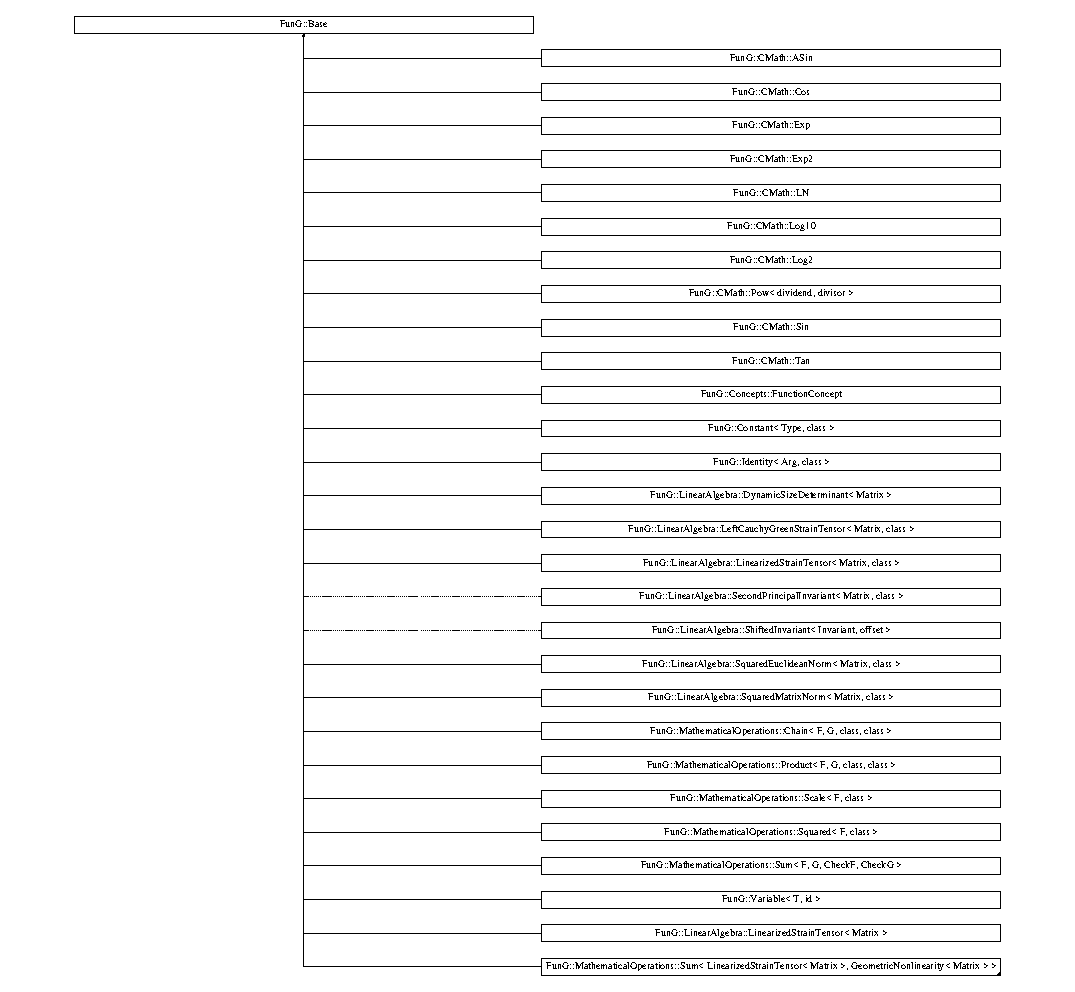
\includegraphics[height=12.000000cm]{structFunG_1_1Base}
\end{center}
\end{figure}


\subsection{Detailed Description}
Base class for functions satisfying Function\+Concept. Required a.\+o. for enabling the operators in \hyperlink{generate_8hh}{generate.\+hh}. 

The documentation for this struct was generated from the following file\+:\begin{DoxyCompactItemize}
\item 
fung/util/\hyperlink{base_8hh}{base.\+hh}\end{DoxyCompactItemize}

\hypertarget{structExample__2_1_1BDiff}{\section{Example\-\_\-2\-:\-:B\-Diff$<$ C $>$ Struct Template Reference}
\label{structExample__2_1_1BDiff}\index{Example\-\_\-2\-::\-B\-Diff$<$ C $>$@{Example\-\_\-2\-::\-B\-Diff$<$ C $>$}}
}
\subsection*{Public Member Functions}
\begin{DoxyCompactItemize}
\item 
\hypertarget{structExample__2_1_1BDiff_aa4baea9ef892c52aeb55438e536a865a}{{\footnotesize template$<$class T $>$ }\\T {\bfseries operator()} (T \&o\-\_\-dfdx, const T \&i\-\_\-x)}\label{structExample__2_1_1BDiff_aa4baea9ef892c52aeb55438e536a865a}

\end{DoxyCompactItemize}


The documentation for this struct was generated from the following file\-:\begin{DoxyCompactItemize}
\item 
fung/tests/A\-D\-Comparison\-\_\-\-Example\-\_\-2.\-hh\end{DoxyCompactItemize}

\hypertarget{structExample__3_1_1BDiff}{\section{Example\-\_\-3\-:\-:B\-Diff$<$ C $>$ Struct Template Reference}
\label{structExample__3_1_1BDiff}\index{Example\-\_\-3\-::\-B\-Diff$<$ C $>$@{Example\-\_\-3\-::\-B\-Diff$<$ C $>$}}
}
\subsection*{Public Member Functions}
\begin{DoxyCompactItemize}
\item 
\hypertarget{structExample__3_1_1BDiff_a646a89c49ab67baf4e49a3bcc9996776}{{\footnotesize template$<$class T $>$ }\\T {\bfseries operator()} (T \&o\-\_\-dfdx, T \&o\-\_\-dfdy, const T \&i\-\_\-x, const T \&i\-\_\-y)}\label{structExample__3_1_1BDiff_a646a89c49ab67baf4e49a3bcc9996776}

\end{DoxyCompactItemize}


The documentation for this struct was generated from the following file\-:\begin{DoxyCompactItemize}
\item 
fung/tests/A\-D\-Comparison\-\_\-\-Example\-\_\-3.\-hh\end{DoxyCompactItemize}

\hypertarget{structADTest_1_1BDiff}{\section{A\-D\-Test\-:\-:B\-Diff$<$ C $>$ Struct Template Reference}
\label{structADTest_1_1BDiff}\index{A\-D\-Test\-::\-B\-Diff$<$ C $>$@{A\-D\-Test\-::\-B\-Diff$<$ C $>$}}
}
\subsection*{Public Member Functions}
\begin{DoxyCompactItemize}
\item 
\hypertarget{structADTest_1_1BDiff_a7c46d215eaaff2b7f9cc9aaf4a0c8899}{{\footnotesize template$<$class T $>$ }\\T {\bfseries operator()} (T \&o\-\_\-dfdx, const T \&i\-\_\-x)}\label{structADTest_1_1BDiff_a7c46d215eaaff2b7f9cc9aaf4a0c8899}

\end{DoxyCompactItemize}


The documentation for this struct was generated from the following file\-:\begin{DoxyCompactItemize}
\item 
fung/tests/A\-D\-Comparison.\-hh\end{DoxyCompactItemize}

\hypertarget{structExample__1_1_1BDiff}{\section{Example\-\_\-1\-:\-:B\-Diff$<$ C $>$ Struct Template Reference}
\label{structExample__1_1_1BDiff}\index{Example\-\_\-1\-::\-B\-Diff$<$ C $>$@{Example\-\_\-1\-::\-B\-Diff$<$ C $>$}}
}
\subsection*{Public Member Functions}
\begin{DoxyCompactItemize}
\item 
\hypertarget{structExample__1_1_1BDiff_a7c9e2208f422f1efaa97d3702bd8e36a}{{\footnotesize template$<$class T $>$ }\\T {\bfseries operator()} (T \&o\-\_\-dfdx, const T \&i\-\_\-x) const }\label{structExample__1_1_1BDiff_a7c9e2208f422f1efaa97d3702bd8e36a}

\end{DoxyCompactItemize}


The documentation for this struct was generated from the following file\-:\begin{DoxyCompactItemize}
\item 
fung/tests/A\-D\-Comparison\-\_\-\-Example\-\_\-1.\-hh\end{DoxyCompactItemize}

\hypertarget{structFunG_1_1MathematicalOperations_1_1Chain}{}\section{FunG\+:\+:Mathematical\+Operations\+:\+:Chain$<$ F, G, class, class $>$ Struct Template Reference}
\label{structFunG_1_1MathematicalOperations_1_1Chain}\index{Fun\+G\+::\+Mathematical\+Operations\+::\+Chain$<$ F, G, class, class $>$@{Fun\+G\+::\+Mathematical\+Operations\+::\+Chain$<$ F, G, class, class $>$}}


Chain $ f\circ g $ of functions $f$ and $g$ of type F resp. G (F and G must satisfy the requirements of \hyperlink{structFunG_1_1Concepts_1_1FunctionConcept}{Concepts\+::\+Function\+Concept}).  




{\ttfamily \#include $<$chain.\+hh$>$}

Inheritance diagram for FunG\+:\+:Mathematical\+Operations\+:\+:Chain$<$ F, G, class, class $>$\+:\begin{figure}[H]
\begin{center}
\leavevmode
\includegraphics[height=1.758242cm]{structFunG_1_1MathematicalOperations_1_1Chain}
\end{center}
\end{figure}
\subsection*{Public Member Functions}
\begin{DoxyCompactItemize}
\item 
\hyperlink{structFunG_1_1MathematicalOperations_1_1Chain_a3167b6304026eb0bd92e57d0dd0087e0}{Chain} (const F \&f\+\_\+, const G \&g\+\_\+)
\begin{DoxyCompactList}\small\item\em Constructor taking copies of the functions to be chained. \end{DoxyCompactList}\item 
\hyperlink{structFunG_1_1MathematicalOperations_1_1Chain_a0c5cc51c17c31db3754edc016a745201}{Chain} (F \&\&f\+\_\+, G \&\&g\+\_\+)
\begin{DoxyCompactList}\small\item\em Constructor taking moving the functions to be chained. \end{DoxyCompactList}\item 
{\footnotesize template$<$class Arg $>$ }\\void \hyperlink{structFunG_1_1MathematicalOperations_1_1Chain_adb7f63859ef7dbdd08b0908c3a17794d}{update} (const Arg \&x)
\begin{DoxyCompactList}\small\item\em Update point of evaluation. \end{DoxyCompactList}\item 
{\footnotesize template$<$int index, class Arg $>$ }\\void \hyperlink{structFunG_1_1MathematicalOperations_1_1Chain_aa41d754e68072e0a9f1460da79f9913e}{update} (const Arg \&x)
\begin{DoxyCompactList}\small\item\em Update variable corresponding to index. \end{DoxyCompactList}\item 
decltype(auto) \hyperlink{structFunG_1_1MathematicalOperations_1_1Chain_a96de3ba6edeb9decba4c04ad9ddb48ff}{d0} () const noexcept
\begin{DoxyCompactList}\small\item\em Function value. \end{DoxyCompactList}\item 
{\footnotesize template$<$int id, class Arg , class Indexed\+Arg  = Indexed\+Type$<$\+Arg,id$>$, class Indexed\+F\+Arg  = Indexed\+Type$<$\+F\+Arg,id$>$, class  = std\+::enable\+\_\+if\+\_\+t$<$ Compute\+Chain\+D1$<$ F , D1$<$\+G,\+Indexed\+Arg$>$ , Indexed\+F\+Arg $>$\+::present$>$$>$ }\\auto \hyperlink{structFunG_1_1MathematicalOperations_1_1Chain_adfe741dee89257258b39df846fd16cf7}{d1} (Arg const \&dx) const 
\begin{DoxyCompactList}\small\item\em First directional derivative. \end{DoxyCompactList}\item 
{\footnotesize template$<$int idx, int idy, class ArgX , class ArgY , class Indexed\+ArgX  = Indexed\+Type$<$\+Arg\+X,idx$>$, class Indexed\+ArgY  = Indexed\+Type$<$\+Arg\+Y,idy$>$, class Indexed\+F\+ArgX  = Indexed\+Type$<$\+F\+Arg,idx$>$, class Indexed\+F\+ArgY  = Indexed\+Type$<$\+F\+Arg,idy$>$, class  = std\+::enable\+\_\+if\+\_\+t$<$ D2\+Lazy\+Type$<$\+Indexed\+Arg\+X,\+Indexed\+Arg\+Y,\+Indexed\+F\+Arg\+X,\+Indexed\+F\+Arg\+Y$>$\+::present $>$$>$ }\\auto \hyperlink{structFunG_1_1MathematicalOperations_1_1Chain_a0ab88c09299ce967583408f7f7dcd2bb}{d2} (ArgX const \&dx, ArgY const \&dy) const 
\begin{DoxyCompactList}\small\item\em Second directional derivative. \end{DoxyCompactList}\item 
{\footnotesize template$<$int idx, int idy, int idz, class ArgX , class ArgY , class ArgZ , class Indexed\+ArgX  = Indexed\+Type$<$\+Arg\+X,idx$>$, class Indexed\+ArgY  = Indexed\+Type$<$\+Arg\+Y,idy$>$, class Indexed\+ArgZ  = Indexed\+Type$<$\+Arg\+Z,idz$>$, class Indexed\+F\+ArgX  = Indexed\+Type$<$\+F\+Arg,idx$>$, class Indexed\+F\+ArgY  = Indexed\+Type$<$\+F\+Arg,idy$>$, class Indexed\+F\+ArgZ  = Indexed\+Type$<$\+F\+Arg,idz$>$, class  = std\+::enable\+\_\+if\+\_\+t$<$ D3\+Lazy\+Type$<$\+Indexed\+Arg\+X,\+Indexed\+Arg\+Y,\+Indexed\+Arg\+Z,\+Indexed\+F\+Arg\+X,\+Indexed\+F\+Arg\+Y,\+Indexed\+F\+Arg\+Z$>$\+::present $>$$>$ }\\auto \hyperlink{structFunG_1_1MathematicalOperations_1_1Chain_a17ac1618545b9d9bd2efa873b36cfbc7}{d3} (ArgX const \&dx, ArgY const \&dy, ArgZ const \&dz) const 
\begin{DoxyCompactList}\small\item\em Third directional derivative. \end{DoxyCompactList}\end{DoxyCompactItemize}


\subsection{Detailed Description}
\subsubsection*{template$<$class F, class G, class = Concepts\+::\+Function\+Concept\+Check$<$\+F$>$, class = Concepts\+::\+Function\+Concept\+Check$<$\+G$>$$>$\\*
struct Fun\+G\+::\+Mathematical\+Operations\+::\+Chain$<$ F, G, class, class $>$}

Chain $ f\circ g $ of functions $f$ and $g$ of type F resp. G (F and G must satisfy the requirements of \hyperlink{structFunG_1_1Concepts_1_1FunctionConcept}{Concepts\+::\+Function\+Concept}). 

\subsection{Constructor \& Destructor Documentation}
\index{Fun\+G\+::\+Mathematical\+Operations\+::\+Chain@{Fun\+G\+::\+Mathematical\+Operations\+::\+Chain}!Chain@{Chain}}
\index{Chain@{Chain}!Fun\+G\+::\+Mathematical\+Operations\+::\+Chain@{Fun\+G\+::\+Mathematical\+Operations\+::\+Chain}}
\subsubsection[{\texorpdfstring{Chain(const F \&f\+\_\+, const G \&g\+\_\+)}{Chain(const F &f_, const G &g_)}}]{\setlength{\rightskip}{0pt plus 5cm}template$<$class F, class G, class  = Concepts\+::\+Function\+Concept\+Check$<$\+F$>$, class  = Concepts\+::\+Function\+Concept\+Check$<$\+G$>$$>$ {\bf Fun\+G\+::\+Mathematical\+Operations\+::\+Chain}$<$ F, G, class, class $>$\+::{\bf Chain} (
\begin{DoxyParamCaption}
\item[{const F \&}]{f\+\_\+, }
\item[{const G \&}]{g\+\_\+}
\end{DoxyParamCaption}
)\hspace{0.3cm}{\ttfamily [inline]}}\hypertarget{structFunG_1_1MathematicalOperations_1_1Chain_a3167b6304026eb0bd92e57d0dd0087e0}{}\label{structFunG_1_1MathematicalOperations_1_1Chain_a3167b6304026eb0bd92e57d0dd0087e0}


Constructor taking copies of the functions to be chained. 


\begin{DoxyParams}{Parameters}
{\em f\+\_\+} & outer function \\
\hline
{\em g\+\_\+} & inner function \\
\hline
\end{DoxyParams}
\index{Fun\+G\+::\+Mathematical\+Operations\+::\+Chain@{Fun\+G\+::\+Mathematical\+Operations\+::\+Chain}!Chain@{Chain}}
\index{Chain@{Chain}!Fun\+G\+::\+Mathematical\+Operations\+::\+Chain@{Fun\+G\+::\+Mathematical\+Operations\+::\+Chain}}
\subsubsection[{\texorpdfstring{Chain(\+F \&\&f\+\_\+, G \&\&g\+\_\+)}{Chain(F &&f_, G &&g_)}}]{\setlength{\rightskip}{0pt plus 5cm}template$<$class F, class G, class  = Concepts\+::\+Function\+Concept\+Check$<$\+F$>$, class  = Concepts\+::\+Function\+Concept\+Check$<$\+G$>$$>$ {\bf Fun\+G\+::\+Mathematical\+Operations\+::\+Chain}$<$ F, G, class, class $>$\+::{\bf Chain} (
\begin{DoxyParamCaption}
\item[{F \&\&}]{f\+\_\+, }
\item[{G \&\&}]{g\+\_\+}
\end{DoxyParamCaption}
)\hspace{0.3cm}{\ttfamily [inline]}}\hypertarget{structFunG_1_1MathematicalOperations_1_1Chain_a0c5cc51c17c31db3754edc016a745201}{}\label{structFunG_1_1MathematicalOperations_1_1Chain_a0c5cc51c17c31db3754edc016a745201}


Constructor taking moving the functions to be chained. 


\begin{DoxyParams}{Parameters}
{\em f\+\_\+} & outer function \\
\hline
{\em g\+\_\+} & inner function \\
\hline
\end{DoxyParams}


\subsection{Member Function Documentation}
\index{Fun\+G\+::\+Mathematical\+Operations\+::\+Chain@{Fun\+G\+::\+Mathematical\+Operations\+::\+Chain}!d0@{d0}}
\index{d0@{d0}!Fun\+G\+::\+Mathematical\+Operations\+::\+Chain@{Fun\+G\+::\+Mathematical\+Operations\+::\+Chain}}
\subsubsection[{\texorpdfstring{d0() const noexcept}{d0() const noexcept}}]{\setlength{\rightskip}{0pt plus 5cm}template$<$class F, class G, class  = Concepts\+::\+Function\+Concept\+Check$<$\+F$>$, class  = Concepts\+::\+Function\+Concept\+Check$<$\+G$>$$>$ decltype(auto) {\bf Fun\+G\+::\+Mathematical\+Operations\+::\+Chain}$<$ F, G, class, class $>$\+::d0 (
\begin{DoxyParamCaption}
{}
\end{DoxyParamCaption}
) const\hspace{0.3cm}{\ttfamily [inline]}, {\ttfamily [noexcept]}}\hypertarget{structFunG_1_1MathematicalOperations_1_1Chain_a96de3ba6edeb9decba4c04ad9ddb48ff}{}\label{structFunG_1_1MathematicalOperations_1_1Chain_a96de3ba6edeb9decba4c04ad9ddb48ff}


Function value. 

\index{Fun\+G\+::\+Mathematical\+Operations\+::\+Chain@{Fun\+G\+::\+Mathematical\+Operations\+::\+Chain}!d1@{d1}}
\index{d1@{d1}!Fun\+G\+::\+Mathematical\+Operations\+::\+Chain@{Fun\+G\+::\+Mathematical\+Operations\+::\+Chain}}
\subsubsection[{\texorpdfstring{d1(\+Arg const \&dx) const }{d1(Arg const &dx) const }}]{\setlength{\rightskip}{0pt plus 5cm}template$<$class F, class G, class  = Concepts\+::\+Function\+Concept\+Check$<$\+F$>$, class  = Concepts\+::\+Function\+Concept\+Check$<$\+G$>$$>$ template$<$int id, class Arg , class Indexed\+Arg  = Indexed\+Type$<$\+Arg,id$>$, class Indexed\+F\+Arg  = Indexed\+Type$<$\+F\+Arg,id$>$, class  = std\+::enable\+\_\+if\+\_\+t$<$ Compute\+Chain\+D1$<$ F , D1$<$\+G,\+Indexed\+Arg$>$ , Indexed\+F\+Arg $>$\+::present$>$$>$ auto {\bf Fun\+G\+::\+Mathematical\+Operations\+::\+Chain}$<$ F, G, class, class $>$\+::d1 (
\begin{DoxyParamCaption}
\item[{Arg const \&}]{dx}
\end{DoxyParamCaption}
) const\hspace{0.3cm}{\ttfamily [inline]}}\hypertarget{structFunG_1_1MathematicalOperations_1_1Chain_adfe741dee89257258b39df846fd16cf7}{}\label{structFunG_1_1MathematicalOperations_1_1Chain_adfe741dee89257258b39df846fd16cf7}


First directional derivative. 


\begin{DoxyParams}{Parameters}
{\em dx} & direction for which the derivative is computed \\
\hline
\end{DoxyParams}
\index{Fun\+G\+::\+Mathematical\+Operations\+::\+Chain@{Fun\+G\+::\+Mathematical\+Operations\+::\+Chain}!d2@{d2}}
\index{d2@{d2}!Fun\+G\+::\+Mathematical\+Operations\+::\+Chain@{Fun\+G\+::\+Mathematical\+Operations\+::\+Chain}}
\subsubsection[{\texorpdfstring{d2(\+Arg\+X const \&dx, Arg\+Y const \&dy) const }{d2(ArgX const &dx, ArgY const &dy) const }}]{\setlength{\rightskip}{0pt plus 5cm}template$<$class F, class G, class  = Concepts\+::\+Function\+Concept\+Check$<$\+F$>$, class  = Concepts\+::\+Function\+Concept\+Check$<$\+G$>$$>$ template$<$int idx, int idy, class ArgX , class ArgY , class Indexed\+ArgX  = Indexed\+Type$<$\+Arg\+X,idx$>$, class Indexed\+ArgY  = Indexed\+Type$<$\+Arg\+Y,idy$>$, class Indexed\+F\+ArgX  = Indexed\+Type$<$\+F\+Arg,idx$>$, class Indexed\+F\+ArgY  = Indexed\+Type$<$\+F\+Arg,idy$>$, class  = std\+::enable\+\_\+if\+\_\+t$<$ D2\+Lazy\+Type$<$\+Indexed\+Arg\+X,\+Indexed\+Arg\+Y,\+Indexed\+F\+Arg\+X,\+Indexed\+F\+Arg\+Y$>$\+::present $>$$>$ auto {\bf Fun\+G\+::\+Mathematical\+Operations\+::\+Chain}$<$ F, G, class, class $>$\+::d2 (
\begin{DoxyParamCaption}
\item[{ArgX const \&}]{dx, }
\item[{ArgY const \&}]{dy}
\end{DoxyParamCaption}
) const\hspace{0.3cm}{\ttfamily [inline]}}\hypertarget{structFunG_1_1MathematicalOperations_1_1Chain_a0ab88c09299ce967583408f7f7dcd2bb}{}\label{structFunG_1_1MathematicalOperations_1_1Chain_a0ab88c09299ce967583408f7f7dcd2bb}


Second directional derivative. 


\begin{DoxyParams}{Parameters}
{\em dx} & direction for which the derivative is computed \\
\hline
{\em dy} & direction for which the derivative is computed \\
\hline
\end{DoxyParams}
\index{Fun\+G\+::\+Mathematical\+Operations\+::\+Chain@{Fun\+G\+::\+Mathematical\+Operations\+::\+Chain}!d3@{d3}}
\index{d3@{d3}!Fun\+G\+::\+Mathematical\+Operations\+::\+Chain@{Fun\+G\+::\+Mathematical\+Operations\+::\+Chain}}
\subsubsection[{\texorpdfstring{d3(\+Arg\+X const \&dx, Arg\+Y const \&dy, Arg\+Z const \&dz) const }{d3(ArgX const &dx, ArgY const &dy, ArgZ const &dz) const }}]{\setlength{\rightskip}{0pt plus 5cm}template$<$class F, class G, class  = Concepts\+::\+Function\+Concept\+Check$<$\+F$>$, class  = Concepts\+::\+Function\+Concept\+Check$<$\+G$>$$>$ template$<$int idx, int idy, int idz, class ArgX , class ArgY , class ArgZ , class Indexed\+ArgX  = Indexed\+Type$<$\+Arg\+X,idx$>$, class Indexed\+ArgY  = Indexed\+Type$<$\+Arg\+Y,idy$>$, class Indexed\+ArgZ  = Indexed\+Type$<$\+Arg\+Z,idz$>$, class Indexed\+F\+ArgX  = Indexed\+Type$<$\+F\+Arg,idx$>$, class Indexed\+F\+ArgY  = Indexed\+Type$<$\+F\+Arg,idy$>$, class Indexed\+F\+ArgZ  = Indexed\+Type$<$\+F\+Arg,idz$>$, class  = std\+::enable\+\_\+if\+\_\+t$<$ D3\+Lazy\+Type$<$\+Indexed\+Arg\+X,\+Indexed\+Arg\+Y,\+Indexed\+Arg\+Z,\+Indexed\+F\+Arg\+X,\+Indexed\+F\+Arg\+Y,\+Indexed\+F\+Arg\+Z$>$\+::present $>$$>$ auto {\bf Fun\+G\+::\+Mathematical\+Operations\+::\+Chain}$<$ F, G, class, class $>$\+::d3 (
\begin{DoxyParamCaption}
\item[{ArgX const \&}]{dx, }
\item[{ArgY const \&}]{dy, }
\item[{ArgZ const \&}]{dz}
\end{DoxyParamCaption}
) const\hspace{0.3cm}{\ttfamily [inline]}}\hypertarget{structFunG_1_1MathematicalOperations_1_1Chain_a17ac1618545b9d9bd2efa873b36cfbc7}{}\label{structFunG_1_1MathematicalOperations_1_1Chain_a17ac1618545b9d9bd2efa873b36cfbc7}


Third directional derivative. 


\begin{DoxyParams}{Parameters}
{\em dx} & direction for which the derivative is computed \\
\hline
{\em dy} & direction for which the derivative is computed \\
\hline
{\em dz} & direction for which the derivative is computed \\
\hline
\end{DoxyParams}
\index{Fun\+G\+::\+Mathematical\+Operations\+::\+Chain@{Fun\+G\+::\+Mathematical\+Operations\+::\+Chain}!update@{update}}
\index{update@{update}!Fun\+G\+::\+Mathematical\+Operations\+::\+Chain@{Fun\+G\+::\+Mathematical\+Operations\+::\+Chain}}
\subsubsection[{\texorpdfstring{update(const Arg \&x)}{update(const Arg &x)}}]{\setlength{\rightskip}{0pt plus 5cm}template$<$class F, class G, class  = Concepts\+::\+Function\+Concept\+Check$<$\+F$>$, class  = Concepts\+::\+Function\+Concept\+Check$<$\+G$>$$>$ template$<$class Arg $>$ void {\bf Fun\+G\+::\+Mathematical\+Operations\+::\+Chain}$<$ F, G, class, class $>$\+::update (
\begin{DoxyParamCaption}
\item[{const Arg \&}]{x}
\end{DoxyParamCaption}
)\hspace{0.3cm}{\ttfamily [inline]}}\hypertarget{structFunG_1_1MathematicalOperations_1_1Chain_adb7f63859ef7dbdd08b0908c3a17794d}{}\label{structFunG_1_1MathematicalOperations_1_1Chain_adb7f63859ef7dbdd08b0908c3a17794d}


Update point of evaluation. 

\index{Fun\+G\+::\+Mathematical\+Operations\+::\+Chain@{Fun\+G\+::\+Mathematical\+Operations\+::\+Chain}!update@{update}}
\index{update@{update}!Fun\+G\+::\+Mathematical\+Operations\+::\+Chain@{Fun\+G\+::\+Mathematical\+Operations\+::\+Chain}}
\subsubsection[{\texorpdfstring{update(const Arg \&x)}{update(const Arg &x)}}]{\setlength{\rightskip}{0pt plus 5cm}template$<$class F, class G, class  = Concepts\+::\+Function\+Concept\+Check$<$\+F$>$, class  = Concepts\+::\+Function\+Concept\+Check$<$\+G$>$$>$ template$<$int index, class Arg $>$ void {\bf Fun\+G\+::\+Mathematical\+Operations\+::\+Chain}$<$ F, G, class, class $>$\+::update (
\begin{DoxyParamCaption}
\item[{const Arg \&}]{x}
\end{DoxyParamCaption}
)\hspace{0.3cm}{\ttfamily [inline]}}\hypertarget{structFunG_1_1MathematicalOperations_1_1Chain_aa41d754e68072e0a9f1460da79f9913e}{}\label{structFunG_1_1MathematicalOperations_1_1Chain_aa41d754e68072e0a9f1460da79f9913e}


Update variable corresponding to index. 



The documentation for this struct was generated from the following file\+:\begin{DoxyCompactItemize}
\item 
fung/mathematical\+\_\+operations/\hyperlink{chain_8hh}{chain.\+hh}\end{DoxyCompactItemize}

\hypertarget{structFunG_1_1Constant}{\section{\-Fun\-G\-:\-:\-Constant$<$ \-Type, class $>$ \-Struct \-Template \-Reference}
\label{structFunG_1_1Constant}\index{\-Fun\-G\-::\-Constant$<$ Type, class $>$@{\-Fun\-G\-::\-Constant$<$ Type, class $>$}}
}


\-Wrap a constant.  




{\ttfamily \#include $<$constant.\-hh$>$}

\subsection*{\-Public \-Member \-Functions}
\begin{DoxyCompactItemize}
\item 
\hyperlink{structFunG_1_1Constant_acdf7efa985ead5b902ec094aaaaef0b8}{\-Constant} ()
\item 
\hyperlink{structFunG_1_1Constant_a310783597f488e554de12627bf56aec8}{\-Constant} (\-Type const \&t\-\_\-)
\begin{DoxyCompactList}\small\item\em \-Construct constant from copy. \end{DoxyCompactList}\item 
const \-Type \& \hyperlink{structFunG_1_1Constant_aad514a9470fbe1c47c0f07da6e160416}{d0} () const noexcept
\begin{DoxyCompactList}\small\item\em \-Function value. \end{DoxyCompactList}\end{DoxyCompactItemize}


\subsection{\-Detailed \-Description}
\subsubsection*{template$<$class Type, class = \-Arithmetic\-Concept\-Check$<$\-Type$>$$>$struct Fun\-G\-::\-Constant$<$ Type, class $>$}

\-Wrap a constant. 

\subsection{\-Constructor \& \-Destructor \-Documentation}
\hypertarget{structFunG_1_1Constant_acdf7efa985ead5b902ec094aaaaef0b8}{\index{\-Fun\-G\-::\-Constant@{\-Fun\-G\-::\-Constant}!\-Constant@{\-Constant}}
\index{\-Constant@{\-Constant}!FunG::Constant@{\-Fun\-G\-::\-Constant}}
\subsubsection[{\-Constant}]{\setlength{\rightskip}{0pt plus 5cm}template$<$class Type , class  = \-Arithmetic\-Concept\-Check$<$\-Type$>$$>$ {\bf \-Fun\-G\-::\-Constant}$<$ \-Type, class $>$\-::{\bf \-Constant} (
\begin{DoxyParamCaption}
{}
\end{DoxyParamCaption}
)}}\label{structFunG_1_1Constant_acdf7efa985ead5b902ec094aaaaef0b8}
\hypertarget{structFunG_1_1Constant_a310783597f488e554de12627bf56aec8}{\index{\-Fun\-G\-::\-Constant@{\-Fun\-G\-::\-Constant}!\-Constant@{\-Constant}}
\index{\-Constant@{\-Constant}!FunG::Constant@{\-Fun\-G\-::\-Constant}}
\subsubsection[{\-Constant}]{\setlength{\rightskip}{0pt plus 5cm}template$<$class Type , class  = \-Arithmetic\-Concept\-Check$<$\-Type$>$$>$ {\bf \-Fun\-G\-::\-Constant}$<$ \-Type, class $>$\-::{\bf \-Constant} (
\begin{DoxyParamCaption}
\item[{\-Type const \&}]{t\-\_\-}
\end{DoxyParamCaption}
)\hspace{0.3cm}{\ttfamily  \mbox{[}inline\mbox{]}}}}\label{structFunG_1_1Constant_a310783597f488e554de12627bf56aec8}


\-Construct constant from copy. 



\subsection{\-Member \-Function \-Documentation}
\hypertarget{structFunG_1_1Constant_aad514a9470fbe1c47c0f07da6e160416}{\index{\-Fun\-G\-::\-Constant@{\-Fun\-G\-::\-Constant}!d0@{d0}}
\index{d0@{d0}!FunG::Constant@{\-Fun\-G\-::\-Constant}}
\subsubsection[{d0}]{\setlength{\rightskip}{0pt plus 5cm}template$<$class Type , class  = \-Arithmetic\-Concept\-Check$<$\-Type$>$$>$ const \-Type\& {\bf \-Fun\-G\-::\-Constant}$<$ \-Type, class $>$\-::{\bf d0} (
\begin{DoxyParamCaption}
{}
\end{DoxyParamCaption}
) const\hspace{0.3cm}{\ttfamily  \mbox{[}inline\mbox{]}}}}\label{structFunG_1_1Constant_aad514a9470fbe1c47c0f07da6e160416}


\-Function value. 



\-The documentation for this struct was generated from the following file\-:\begin{DoxyCompactItemize}
\item 
fung/\hyperlink{constant_8hh}{constant.\-hh}\end{DoxyCompactItemize}

\hypertarget{structFunG_1_1Concepts_1_1CopyConcept}{\section{Fun\-G\-:\-:Concepts\-:\-:Copy\-Concept Struct Reference}
\label{structFunG_1_1Concepts_1_1CopyConcept}\index{Fun\-G\-::\-Concepts\-::\-Copy\-Concept@{Fun\-G\-::\-Concepts\-::\-Copy\-Concept}}
}


Requires copy-\/constructibility and copy-\/assignability.  




{\ttfamily \#include $<$concepts.\-hh$>$}

Inheritance diagram for Fun\-G\-:\-:Concepts\-:\-:Copy\-Concept\-:\begin{figure}[H]
\begin{center}
\leavevmode
\includegraphics[height=2.187500cm]{structFunG_1_1Concepts_1_1CopyConcept}
\end{center}
\end{figure}
\subsection*{Public Member Functions}
\begin{DoxyCompactItemize}
\item 
\hypertarget{structFunG_1_1Concepts_1_1CopyConcept_afc08741d422ff46c2e681efc38913144}{\hyperlink{structFunG_1_1Concepts_1_1CopyConcept_afc08741d422ff46c2e681efc38913144}{Copy\-Concept} (const \hyperlink{structFunG_1_1Concepts_1_1CopyConcept}{Copy\-Concept} \&)}\label{structFunG_1_1Concepts_1_1CopyConcept_afc08741d422ff46c2e681efc38913144}

\begin{DoxyCompactList}\small\item\em Copy-\/constructible. \end{DoxyCompactList}\item 
\hypertarget{structFunG_1_1Concepts_1_1CopyConcept_a43c6c112f8164497a4279458af2c0b20}{\hyperlink{structFunG_1_1Concepts_1_1CopyConcept}{Copy\-Concept} \& \hyperlink{structFunG_1_1Concepts_1_1CopyConcept_a43c6c112f8164497a4279458af2c0b20}{operator=} (const \hyperlink{structFunG_1_1Concepts_1_1CopyConcept}{Copy\-Concept} \&)}\label{structFunG_1_1Concepts_1_1CopyConcept_a43c6c112f8164497a4279458af2c0b20}

\begin{DoxyCompactList}\small\item\em Copy-\/assignable. \end{DoxyCompactList}\end{DoxyCompactItemize}


\subsection{Detailed Description}
Requires copy-\/constructibility and copy-\/assignability. 

The documentation for this struct was generated from the following file\-:\begin{DoxyCompactItemize}
\item 
Fun\-G/\hyperlink{concepts_8hh}{concepts.\-hh}\end{DoxyCompactItemize}

\hypertarget{structFunG_1_1Concepts_1_1CopyConceptCheck}{\section{\-Fun\-G\-:\-:\-Concepts\-:\-:\-Copy\-Concept\-Check$<$ \-Arg $>$ \-Struct \-Template \-Reference}
\label{structFunG_1_1Concepts_1_1CopyConceptCheck}\index{\-Fun\-G\-::\-Concepts\-::\-Copy\-Concept\-Check$<$ Arg $>$@{\-Fun\-G\-::\-Concepts\-::\-Copy\-Concept\-Check$<$ Arg $>$}}
}


\-Static check if the requirements of \hyperlink{structFunG_1_1Concepts_1_1CopyConcept}{\-Copy\-Concept} are satisfied.  




{\ttfamily \#include $<$concept\-\_\-check.\-hh$>$}

\-Inheritance diagram for \-Fun\-G\-:\-:\-Concepts\-:\-:\-Copy\-Concept\-Check$<$ \-Arg $>$\-:\begin{figure}[H]
\begin{center}
\leavevmode
\includegraphics[height=2.000000cm]{structFunG_1_1Concepts_1_1CopyConceptCheck}
\end{center}
\end{figure}
\subsection*{\-Public \-Member \-Functions}
\begin{DoxyCompactItemize}
\item 
\hyperlink{structFunG_1_1Concepts_1_1CopyConceptCheck_aa471b5bea12828b79bc4d365745d3373}{static\-\_\-assert} (std\-::is\-\_\-copy\-\_\-constructible$<$ \-Arg $>$(),\char`\"{}\-Copy\-Concept\-: \-Input types must be copy-\/constructible.\char`\"{})
\end{DoxyCompactItemize}


\subsection{\-Detailed \-Description}
\subsubsection*{template$<$class \-Arg$>$struct Fun\-G\-::\-Concepts\-::\-Copy\-Concept\-Check$<$ Arg $>$}

\-Static check if the requirements of \hyperlink{structFunG_1_1Concepts_1_1CopyConcept}{\-Copy\-Concept} are satisfied. 

\subsection{\-Member \-Function \-Documentation}
\hypertarget{structFunG_1_1Concepts_1_1CopyConceptCheck_aa471b5bea12828b79bc4d365745d3373}{\index{\-Fun\-G\-::\-Concepts\-::\-Copy\-Concept\-Check@{\-Fun\-G\-::\-Concepts\-::\-Copy\-Concept\-Check}!static\-\_\-assert@{static\-\_\-assert}}
\index{static\-\_\-assert@{static\-\_\-assert}!FunG::Concepts::CopyConceptCheck@{\-Fun\-G\-::\-Concepts\-::\-Copy\-Concept\-Check}}
\subsubsection[{static\-\_\-assert}]{\setlength{\rightskip}{0pt plus 5cm}template$<$class \-Arg$>$ {\bf \-Fun\-G\-::\-Concepts\-::\-Copy\-Concept\-Check}$<$ \-Arg $>$\-::{\bf static\-\_\-assert} (
\begin{DoxyParamCaption}
\item[{std\-::is\-\_\-copy\-\_\-constructible$<$ \-Arg $>$}]{(), }
\item[{\char`\"{}\-Copy\-Concept\-: \-Input types must be copy-\/constructible.\char`\"{}}]{}
\end{DoxyParamCaption}
)}}\label{structFunG_1_1Concepts_1_1CopyConceptCheck_aa471b5bea12828b79bc4d365745d3373}


\-The documentation for this struct was generated from the following file\-:\begin{DoxyCompactItemize}
\item 
fung/\hyperlink{concept__check_8hh}{concept\-\_\-check.\-hh}\end{DoxyCompactItemize}

\hypertarget{structFunG_1_1CMath_1_1Cos}{\section{Fun\-G\-:\-:C\-Math\-:\-:Cos Struct Reference}
\label{structFunG_1_1CMath_1_1Cos}\index{Fun\-G\-::\-C\-Math\-::\-Cos@{Fun\-G\-::\-C\-Math\-::\-Cos}}
}


Cosine function including first three derivatives (based on cos(double) in $<$cmath$>$).  




{\ttfamily \#include $<$cosine.\-hh$>$}

Inheritance diagram for Fun\-G\-:\-:C\-Math\-:\-:Cos\-:\begin{figure}[H]
\begin{center}
\leavevmode
\includegraphics[height=2.000000cm]{structFunG_1_1CMath_1_1Cos}
\end{center}
\end{figure}
\subsection*{Public Member Functions}
\begin{DoxyCompactItemize}
\item 
\hyperlink{structFunG_1_1CMath_1_1Cos_a0141b060cf225e312688d83cc4755405}{Cos} (double x=0.)
\begin{DoxyCompactList}\small\item\em Constructor. \end{DoxyCompactList}\item 
\hypertarget{structFunG_1_1CMath_1_1Cos_a8b05d39c50e40f56860992fff6f1b807}{void \hyperlink{structFunG_1_1CMath_1_1Cos_a8b05d39c50e40f56860992fff6f1b807}{update} (const double \&x)}\label{structFunG_1_1CMath_1_1Cos_a8b05d39c50e40f56860992fff6f1b807}

\begin{DoxyCompactList}\small\item\em Reset point of evaluation. \end{DoxyCompactList}\item 
\hypertarget{structFunG_1_1CMath_1_1Cos_aa46877147699c4cc83edf12748ac350b}{double \hyperlink{structFunG_1_1CMath_1_1Cos_aa46877147699c4cc83edf12748ac350b}{d0} () const noexcept}\label{structFunG_1_1CMath_1_1Cos_aa46877147699c4cc83edf12748ac350b}

\begin{DoxyCompactList}\small\item\em Function value. \end{DoxyCompactList}\item 
\hypertarget{structFunG_1_1CMath_1_1Cos_a2db41e7d2e1cf7491b4383de9fd3c57e}{{\footnotesize template$<$int  = -\/1$>$ }\\double \hyperlink{structFunG_1_1CMath_1_1Cos_a2db41e7d2e1cf7491b4383de9fd3c57e}{d1} (double dx=1.) const }\label{structFunG_1_1CMath_1_1Cos_a2db41e7d2e1cf7491b4383de9fd3c57e}

\begin{DoxyCompactList}\small\item\em First (directional) derivative. \end{DoxyCompactList}\item 
\hypertarget{structFunG_1_1CMath_1_1Cos_a1a93453bbcd2dfee78a77a43df905a17}{{\footnotesize template$<$int  = -\/1, int  = -\/1$>$ }\\double \hyperlink{structFunG_1_1CMath_1_1Cos_a1a93453bbcd2dfee78a77a43df905a17}{d2} (double dx=1., double dy=1.) const }\label{structFunG_1_1CMath_1_1Cos_a1a93453bbcd2dfee78a77a43df905a17}

\begin{DoxyCompactList}\small\item\em Second (directional) derivative. \end{DoxyCompactList}\item 
\hypertarget{structFunG_1_1CMath_1_1Cos_af364a2b9fa5a34f249e281c5f83363c2}{{\footnotesize template$<$int  = -\/1, int  = -\/1, int  = -\/1$>$ }\\double \hyperlink{structFunG_1_1CMath_1_1Cos_af364a2b9fa5a34f249e281c5f83363c2}{d3} (double dx=1., double dy=1., double dz=1.) const }\label{structFunG_1_1CMath_1_1Cos_af364a2b9fa5a34f249e281c5f83363c2}

\begin{DoxyCompactList}\small\item\em Third (directional) derivative. \end{DoxyCompactList}\end{DoxyCompactItemize}


\subsection{Detailed Description}
Cosine function including first three derivatives (based on cos(double) in $<$cmath$>$). 

For scalar functions directional derivatives are less interesting. Incorporating this function as building block for more complex functions requires directional derivatives. These occur during applications of the chain rule.

\begin{DoxySeeAlso}{See Also}
cosine 
\end{DoxySeeAlso}


\subsection{Constructor \& Destructor Documentation}
\hypertarget{structFunG_1_1CMath_1_1Cos_a0141b060cf225e312688d83cc4755405}{\index{Fun\-G\-::\-C\-Math\-::\-Cos@{Fun\-G\-::\-C\-Math\-::\-Cos}!Cos@{Cos}}
\index{Cos@{Cos}!FunG::CMath::Cos@{Fun\-G\-::\-C\-Math\-::\-Cos}}
\subsubsection[{Cos}]{\setlength{\rightskip}{0pt plus 5cm}Fun\-G\-::\-C\-Math\-::\-Cos\-::\-Cos (
\begin{DoxyParamCaption}
\item[{double}]{x = {\ttfamily 0.}}
\end{DoxyParamCaption}
)\hspace{0.3cm}{\ttfamily [inline]}, {\ttfamily [explicit]}}}\label{structFunG_1_1CMath_1_1Cos_a0141b060cf225e312688d83cc4755405}


Constructor. 


\begin{DoxyParams}{Parameters}
{\em x} & point of evaluation \\
\hline
\end{DoxyParams}


The documentation for this struct was generated from the following file\-:\begin{DoxyCompactItemize}
\item 
fung/cmath/cosine.\-hh\end{DoxyCompactItemize}

\hypertarget{classFunG_1_1LinearAlgebra_1_1Deviator}{\section{Fun\-G\-:\-:Linear\-Algebra\-:\-:Deviator$<$ Matrix $>$ Class Template Reference}
\label{classFunG_1_1LinearAlgebra_1_1Deviator}\index{Fun\-G\-::\-Linear\-Algebra\-::\-Deviator$<$ Matrix $>$@{Fun\-G\-::\-Linear\-Algebra\-::\-Deviator$<$ Matrix $>$}}
}


Type of the deviator of a matrix $ A\in\mathbb{R}^{n,n} $, i.\-e. $ A - \frac{\mathrm{tr}(A)}{n}I $.  




{\ttfamily \#include $<$deviator.\-hh$>$}

Inheritance diagram for Fun\-G\-:\-:Linear\-Algebra\-:\-:Deviator$<$ Matrix $>$\-:\begin{figure}[H]
\begin{center}
\leavevmode
\includegraphics[height=2.000000cm]{classFunG_1_1LinearAlgebra_1_1Deviator}
\end{center}
\end{figure}
\subsection*{Public Member Functions}
\begin{DoxyCompactItemize}
\item 
\hypertarget{classFunG_1_1LinearAlgebra_1_1Deviator_a5baa30ab51f9b03563378bf288d8f648}{{\bfseries Deviator} (const Matrix \&A)}\label{classFunG_1_1LinearAlgebra_1_1Deviator_a5baa30ab51f9b03563378bf288d8f648}

\end{DoxyCompactItemize}


\subsection{Detailed Description}
\subsubsection*{template$<$class Matrix$>$class Fun\-G\-::\-Linear\-Algebra\-::\-Deviator$<$ Matrix $>$}

Type of the deviator of a matrix $ A\in\mathbb{R}^{n,n} $, i.\-e. $ A - \frac{\mathrm{tr}(A)}{n}I $. 

The documentation for this class was generated from the following file\-:\begin{DoxyCompactItemize}
\item 
Fun\-G/\-Linear\-Algebra/deviator.\-hh\end{DoxyCompactItemize}

\hypertarget{classFunG_1_1LinearAlgebra_1_1DynamicSizeDeterminant}{\section{Fun\-G\-:\-:Linear\-Algebra\-:\-:Dynamic\-Size\-Determinant$<$ Matrix $>$ Class Template Reference}
\label{classFunG_1_1LinearAlgebra_1_1DynamicSizeDeterminant}\index{Fun\-G\-::\-Linear\-Algebra\-::\-Dynamic\-Size\-Determinant$<$ Matrix $>$@{Fun\-G\-::\-Linear\-Algebra\-::\-Dynamic\-Size\-Determinant$<$ Matrix $>$}}
}


Determinant of dynamic size matrix with first three derivatives.  




{\ttfamily \#include $<$determinant.\-hh$>$}

Inheritance diagram for Fun\-G\-:\-:Linear\-Algebra\-:\-:Dynamic\-Size\-Determinant$<$ Matrix $>$\-:\begin{figure}[H]
\begin{center}
\leavevmode
\includegraphics[height=1.632653cm]{classFunG_1_1LinearAlgebra_1_1DynamicSizeDeterminant}
\end{center}
\end{figure}
\subsection*{Public Member Functions}
\begin{DoxyCompactItemize}
\item 
\hypertarget{classFunG_1_1LinearAlgebra_1_1DynamicSizeDeterminant_a731ffc80bbf7b4ad98928ada0a665c79}{\hyperlink{classFunG_1_1LinearAlgebra_1_1DynamicSizeDeterminant_a731ffc80bbf7b4ad98928ada0a665c79}{Dynamic\-Size\-Determinant} (Matrix const \&A)}\label{classFunG_1_1LinearAlgebra_1_1DynamicSizeDeterminant_a731ffc80bbf7b4ad98928ada0a665c79}

\begin{DoxyCompactList}\small\item\em Constructor. \end{DoxyCompactList}\item 
\hypertarget{classFunG_1_1LinearAlgebra_1_1DynamicSizeDeterminant_a3f9383818a6b5c21e7c618fc8020ffed}{void \hyperlink{classFunG_1_1LinearAlgebra_1_1DynamicSizeDeterminant_a3f9383818a6b5c21e7c618fc8020ffed}{update} (Matrix const \&A)}\label{classFunG_1_1LinearAlgebra_1_1DynamicSizeDeterminant_a3f9383818a6b5c21e7c618fc8020ffed}

\begin{DoxyCompactList}\small\item\em Reset point of evaluation. \end{DoxyCompactList}\item 
\hypertarget{classFunG_1_1LinearAlgebra_1_1DynamicSizeDeterminant_a5c1835202a0712c2606088271835c485}{auto \hyperlink{classFunG_1_1LinearAlgebra_1_1DynamicSizeDeterminant_a5c1835202a0712c2606088271835c485}{d0} () const }\label{classFunG_1_1LinearAlgebra_1_1DynamicSizeDeterminant_a5c1835202a0712c2606088271835c485}

\begin{DoxyCompactList}\small\item\em Function value. \end{DoxyCompactList}\item 
\hypertarget{classFunG_1_1LinearAlgebra_1_1DynamicSizeDeterminant_a41bc32f2131ed1b6d61f6b0f27f1bc22}{{\footnotesize template$<$int id$>$ }\\auto \hyperlink{classFunG_1_1LinearAlgebra_1_1DynamicSizeDeterminant_a41bc32f2131ed1b6d61f6b0f27f1bc22}{d1} (Matrix const \&d\-A1) const }\label{classFunG_1_1LinearAlgebra_1_1DynamicSizeDeterminant_a41bc32f2131ed1b6d61f6b0f27f1bc22}

\begin{DoxyCompactList}\small\item\em First (directional) derivative. \end{DoxyCompactList}\item 
\hypertarget{classFunG_1_1LinearAlgebra_1_1DynamicSizeDeterminant_a012fc1b7e116b65af25bf7985cecfcc1}{{\footnotesize template$<$int idx, int idy$>$ }\\auto \hyperlink{classFunG_1_1LinearAlgebra_1_1DynamicSizeDeterminant_a012fc1b7e116b65af25bf7985cecfcc1}{d2} (Matrix const \&d\-A1, Matrix const \&d\-A2) const }\label{classFunG_1_1LinearAlgebra_1_1DynamicSizeDeterminant_a012fc1b7e116b65af25bf7985cecfcc1}

\begin{DoxyCompactList}\small\item\em Second (directional) derivative. \end{DoxyCompactList}\item 
\hypertarget{classFunG_1_1LinearAlgebra_1_1DynamicSizeDeterminant_a9cadc3d8e2332f153f3f7e9c93232333}{{\footnotesize template$<$int idx, int idy, int idz$>$ }\\auto \hyperlink{classFunG_1_1LinearAlgebra_1_1DynamicSizeDeterminant_a9cadc3d8e2332f153f3f7e9c93232333}{d3} (Matrix const \&d\-A1, Matrix const \&d\-A2, Matrix const \&d\-A3) const }\label{classFunG_1_1LinearAlgebra_1_1DynamicSizeDeterminant_a9cadc3d8e2332f153f3f7e9c93232333}

\begin{DoxyCompactList}\small\item\em Third (directional) derivative. \end{DoxyCompactList}\end{DoxyCompactItemize}


\subsection{Detailed Description}
\subsubsection*{template$<$class Matrix$>$class Fun\-G\-::\-Linear\-Algebra\-::\-Dynamic\-Size\-Determinant$<$ Matrix $>$}

Determinant of dynamic size matrix with first three derivatives. 

The documentation for this class was generated from the following file\-:\begin{DoxyCompactItemize}
\item 
fung/linear\-\_\-algebra/determinant.\-hh\end{DoxyCompactItemize}

\hypertarget{structFunG_1_1CMath_1_1Exp}{\section{Fun\-G\-:\-:C\-Math\-:\-:Exp Struct Reference}
\label{structFunG_1_1CMath_1_1Exp}\index{Fun\-G\-::\-C\-Math\-::\-Exp@{Fun\-G\-::\-C\-Math\-::\-Exp}}
}


Exponential function including first three derivatives.  




{\ttfamily \#include $<$exp.\-hh$>$}

Inheritance diagram for Fun\-G\-:\-:C\-Math\-:\-:Exp\-:\begin{figure}[H]
\begin{center}
\leavevmode
\includegraphics[height=2.000000cm]{structFunG_1_1CMath_1_1Exp}
\end{center}
\end{figure}
\subsection*{Public Member Functions}
\begin{DoxyCompactItemize}
\item 
\hyperlink{structFunG_1_1CMath_1_1Exp_af565af377733457d1ab31496bdd94cfc}{Exp} (double x=0.)
\begin{DoxyCompactList}\small\item\em Constructor. \end{DoxyCompactList}\item 
\hypertarget{structFunG_1_1CMath_1_1Exp_afc527a1d24bc47c2ed924b7cbbf4e292}{void \hyperlink{structFunG_1_1CMath_1_1Exp_afc527a1d24bc47c2ed924b7cbbf4e292}{update} (double x)}\label{structFunG_1_1CMath_1_1Exp_afc527a1d24bc47c2ed924b7cbbf4e292}

\begin{DoxyCompactList}\small\item\em Reset point of evaluation. \end{DoxyCompactList}\item 
\hypertarget{structFunG_1_1CMath_1_1Exp_a21a4abcf4945372e3154d65dc19ad4b6}{double \hyperlink{structFunG_1_1CMath_1_1Exp_a21a4abcf4945372e3154d65dc19ad4b6}{d0} () const noexcept}\label{structFunG_1_1CMath_1_1Exp_a21a4abcf4945372e3154d65dc19ad4b6}

\begin{DoxyCompactList}\small\item\em Function value. \end{DoxyCompactList}\item 
\hypertarget{structFunG_1_1CMath_1_1Exp_a547f04d65ffdb6ba38508410a864faec}{{\footnotesize template$<$int  = -\/1$>$ }\\double \hyperlink{structFunG_1_1CMath_1_1Exp_a547f04d65ffdb6ba38508410a864faec}{d1} (double dx=1.) const }\label{structFunG_1_1CMath_1_1Exp_a547f04d65ffdb6ba38508410a864faec}

\begin{DoxyCompactList}\small\item\em First (directional) derivative. \end{DoxyCompactList}\item 
\hypertarget{structFunG_1_1CMath_1_1Exp_ad65767da6e7345bd017827b84d9e48cf}{{\footnotesize template$<$int  = -\/1, int  = -\/1$>$ }\\double \hyperlink{structFunG_1_1CMath_1_1Exp_ad65767da6e7345bd017827b84d9e48cf}{d2} (double dx=1., double dy=1.) const }\label{structFunG_1_1CMath_1_1Exp_ad65767da6e7345bd017827b84d9e48cf}

\begin{DoxyCompactList}\small\item\em Second (directinal) derivative. \end{DoxyCompactList}\item 
\hypertarget{structFunG_1_1CMath_1_1Exp_a80da057222d42dfbfaba4d7fa9dbfda2}{{\footnotesize template$<$int  = -\/1, int  = -\/1, int  = -\/1$>$ }\\double \hyperlink{structFunG_1_1CMath_1_1Exp_a80da057222d42dfbfaba4d7fa9dbfda2}{d3} (double dx=1., double dy=1., double dz=1.) const }\label{structFunG_1_1CMath_1_1Exp_a80da057222d42dfbfaba4d7fa9dbfda2}

\begin{DoxyCompactList}\small\item\em Third (directional) derivative. \end{DoxyCompactList}\end{DoxyCompactItemize}


\subsection{Detailed Description}
Exponential function including first three derivatives. 

For scalar functions directional derivatives are less interesting. Incorporating this function as building block for more complex functions requires directional derivatives. These occur during applications of the chain rule. 

\subsection{Constructor \& Destructor Documentation}
\hypertarget{structFunG_1_1CMath_1_1Exp_af565af377733457d1ab31496bdd94cfc}{\index{Fun\-G\-::\-C\-Math\-::\-Exp@{Fun\-G\-::\-C\-Math\-::\-Exp}!Exp@{Exp}}
\index{Exp@{Exp}!FunG::CMath::Exp@{Fun\-G\-::\-C\-Math\-::\-Exp}}
\subsubsection[{Exp}]{\setlength{\rightskip}{0pt plus 5cm}Fun\-G\-::\-C\-Math\-::\-Exp\-::\-Exp (
\begin{DoxyParamCaption}
\item[{double}]{x = {\ttfamily 0.}}
\end{DoxyParamCaption}
)\hspace{0.3cm}{\ttfamily [inline]}, {\ttfamily [explicit]}}}\label{structFunG_1_1CMath_1_1Exp_af565af377733457d1ab31496bdd94cfc}


Constructor. 


\begin{DoxyParams}{Parameters}
{\em x} & point of evaluation \\
\hline
\end{DoxyParams}


The documentation for this struct was generated from the following file\-:\begin{DoxyCompactItemize}
\item 
fung/cmath/exp.\-hh\end{DoxyCompactItemize}

\hypertarget{structFunG_1_1CMath_1_1Exp2}{\section{Fun\-G\-:\-:C\-Math\-:\-:Exp2 Struct Reference}
\label{structFunG_1_1CMath_1_1Exp2}\index{Fun\-G\-::\-C\-Math\-::\-Exp2@{Fun\-G\-::\-C\-Math\-::\-Exp2}}
}


Function $2^x$ including first three derivatives.  




{\ttfamily \#include $<$exp.\-hh$>$}

Inheritance diagram for Fun\-G\-:\-:C\-Math\-:\-:Exp2\-:\begin{figure}[H]
\begin{center}
\leavevmode
\includegraphics[height=2.000000cm]{structFunG_1_1CMath_1_1Exp2}
\end{center}
\end{figure}
\subsection*{Public Member Functions}
\begin{DoxyCompactItemize}
\item 
\hyperlink{structFunG_1_1CMath_1_1Exp2_a9fab717beacdbfed65c40bd36c51ef00}{Exp2} (double x=0.)
\begin{DoxyCompactList}\small\item\em Constructor. \end{DoxyCompactList}\item 
\hypertarget{structFunG_1_1CMath_1_1Exp2_a580df08ee1b7b090c83ec45c90c88927}{void \hyperlink{structFunG_1_1CMath_1_1Exp2_a580df08ee1b7b090c83ec45c90c88927}{update} (double x)}\label{structFunG_1_1CMath_1_1Exp2_a580df08ee1b7b090c83ec45c90c88927}

\begin{DoxyCompactList}\small\item\em Reset point of evaluation. \end{DoxyCompactList}\item 
\hypertarget{structFunG_1_1CMath_1_1Exp2_a035ec564f0f3309ebe1b3049e26c81f6}{double \hyperlink{structFunG_1_1CMath_1_1Exp2_a035ec564f0f3309ebe1b3049e26c81f6}{d0} () const noexcept}\label{structFunG_1_1CMath_1_1Exp2_a035ec564f0f3309ebe1b3049e26c81f6}

\begin{DoxyCompactList}\small\item\em Function value. \end{DoxyCompactList}\item 
\hypertarget{structFunG_1_1CMath_1_1Exp2_a3715733c2d753308bd3884f2d83ac3b0}{{\footnotesize template$<$int  = -\/1$>$ }\\double \hyperlink{structFunG_1_1CMath_1_1Exp2_a3715733c2d753308bd3884f2d83ac3b0}{d1} (double dx=1.) const }\label{structFunG_1_1CMath_1_1Exp2_a3715733c2d753308bd3884f2d83ac3b0}

\begin{DoxyCompactList}\small\item\em First (directional) derivative. \end{DoxyCompactList}\item 
\hypertarget{structFunG_1_1CMath_1_1Exp2_a6fa6c2b7017fb6089937a61871b6f5fd}{{\footnotesize template$<$int  = -\/1, int  = -\/1$>$ }\\double \hyperlink{structFunG_1_1CMath_1_1Exp2_a6fa6c2b7017fb6089937a61871b6f5fd}{d2} (double dx=1., double dy=1.) const }\label{structFunG_1_1CMath_1_1Exp2_a6fa6c2b7017fb6089937a61871b6f5fd}

\begin{DoxyCompactList}\small\item\em Second (directinal) derivative. \end{DoxyCompactList}\item 
\hypertarget{structFunG_1_1CMath_1_1Exp2_a893c27f99eec069ea86807be396b220f}{{\footnotesize template$<$int  = -\/1, int  = -\/1, int  = -\/1$>$ }\\double \hyperlink{structFunG_1_1CMath_1_1Exp2_a893c27f99eec069ea86807be396b220f}{d3} (double dx=1., double dy=1., double dz=1.) const }\label{structFunG_1_1CMath_1_1Exp2_a893c27f99eec069ea86807be396b220f}

\begin{DoxyCompactList}\small\item\em Third (directional) derivative. \end{DoxyCompactList}\end{DoxyCompactItemize}


\subsection{Detailed Description}
Function $2^x$ including first three derivatives. 

For scalar functions directional derivatives are less interesting. Incorporating this function as building block for more complex functions requires directional derivatives. These occur during applications of the chain rule. 

\subsection{Constructor \& Destructor Documentation}
\hypertarget{structFunG_1_1CMath_1_1Exp2_a9fab717beacdbfed65c40bd36c51ef00}{\index{Fun\-G\-::\-C\-Math\-::\-Exp2@{Fun\-G\-::\-C\-Math\-::\-Exp2}!Exp2@{Exp2}}
\index{Exp2@{Exp2}!FunG::CMath::Exp2@{Fun\-G\-::\-C\-Math\-::\-Exp2}}
\subsubsection[{Exp2}]{\setlength{\rightskip}{0pt plus 5cm}Fun\-G\-::\-C\-Math\-::\-Exp2\-::\-Exp2 (
\begin{DoxyParamCaption}
\item[{double}]{x = {\ttfamily 0.}}
\end{DoxyParamCaption}
)\hspace{0.3cm}{\ttfamily [inline]}, {\ttfamily [explicit]}}}\label{structFunG_1_1CMath_1_1Exp2_a9fab717beacdbfed65c40bd36c51ef00}


Constructor. 


\begin{DoxyParams}{Parameters}
{\em x} & point of evaluation \\
\hline
\end{DoxyParams}


The documentation for this struct was generated from the following file\-:\begin{DoxyCompactItemize}
\item 
Fun\-G/\-C\-Math/exp.\-hh\end{DoxyCompactItemize}

\hypertarget{structExample__2_1_1FDiff}{\section{Example\-\_\-2\-:\-:F\-Diff$<$ C $>$ Struct Template Reference}
\label{structExample__2_1_1FDiff}\index{Example\-\_\-2\-::\-F\-Diff$<$ C $>$@{Example\-\_\-2\-::\-F\-Diff$<$ C $>$}}
}
\subsection*{Public Member Functions}
\begin{DoxyCompactItemize}
\item 
\hypertarget{structExample__2_1_1FDiff_a9399c3f33cdd14a9f65795921f632888}{{\footnotesize template$<$typename T $>$ }\\T {\bfseries operator()} (T \&o\-\_\-dfdx, const T \&i\-\_\-x)}\label{structExample__2_1_1FDiff_a9399c3f33cdd14a9f65795921f632888}

\end{DoxyCompactItemize}


The documentation for this struct was generated from the following file\-:\begin{DoxyCompactItemize}
\item 
fung/tests/A\-D\-Comparison\-\_\-\-Example\-\_\-2.\-hh\end{DoxyCompactItemize}

\hypertarget{structExample__3_1_1FDiff}{\section{Example\-\_\-3\-:\-:F\-Diff$<$ C $>$ Struct Template Reference}
\label{structExample__3_1_1FDiff}\index{Example\-\_\-3\-::\-F\-Diff$<$ C $>$@{Example\-\_\-3\-::\-F\-Diff$<$ C $>$}}
}
\subsection*{Public Member Functions}
\begin{DoxyCompactItemize}
\item 
\hypertarget{structExample__3_1_1FDiff_ad72a19157aef8110a55462ebcc85d988}{{\footnotesize template$<$typename T $>$ }\\T {\bfseries operator()} (T \&o\-\_\-dfdx, T \&o\-\_\-dfdy, const T \&i\-\_\-x, const T \&i\-\_\-y)}\label{structExample__3_1_1FDiff_ad72a19157aef8110a55462ebcc85d988}

\end{DoxyCompactItemize}


The documentation for this struct was generated from the following file\-:\begin{DoxyCompactItemize}
\item 
fung/tests/A\-D\-Comparison\-\_\-\-Example\-\_\-3.\-hh\end{DoxyCompactItemize}

\hypertarget{structExample__5_1_1FDiff}{\section{Example\-\_\-5\-:\-:F\-Diff$<$ C $>$ Struct Template Reference}
\label{structExample__5_1_1FDiff}\index{Example\-\_\-5\-::\-F\-Diff$<$ C $>$@{Example\-\_\-5\-::\-F\-Diff$<$ C $>$}}
}
\subsection*{Public Member Functions}
\begin{DoxyCompactItemize}
\item 
\hypertarget{structExample__5_1_1FDiff_aefb29923f0a8b9f3b0f9a52dae41b4bb}{{\footnotesize template$<$typename T0 , typename T1 $>$ }\\auto {\bfseries operator()} (T0 \&o\-\_\-dfdx, const T1 \&i\-\_\-x) const }\label{structExample__5_1_1FDiff_aefb29923f0a8b9f3b0f9a52dae41b4bb}

\end{DoxyCompactItemize}


The documentation for this struct was generated from the following file\-:\begin{DoxyCompactItemize}
\item 
fung/tests/A\-D\-Comparison\-\_\-\-Example\-\_\-5.\-hh\end{DoxyCompactItemize}

\hypertarget{structExample__4_1_1FDiff}{\section{Example\-\_\-4\-:\-:F\-Diff$<$ C $>$ Struct Template Reference}
\label{structExample__4_1_1FDiff}\index{Example\-\_\-4\-::\-F\-Diff$<$ C $>$@{Example\-\_\-4\-::\-F\-Diff$<$ C $>$}}
}
\subsection*{Public Member Functions}
\begin{DoxyCompactItemize}
\item 
\hypertarget{structExample__4_1_1FDiff_af13f7f08c32a9ef4189c39aa8fb7faf0}{{\footnotesize template$<$typename T0 , typename T1 $>$ }\\auto {\bfseries operator()} (T0 \&o\-\_\-dfdx, T0 \&o\-\_\-dfdy, const T0 \&i\-\_\-x, const T1 \&i\-\_\-y) const }\label{structExample__4_1_1FDiff_af13f7f08c32a9ef4189c39aa8fb7faf0}

\end{DoxyCompactItemize}


The documentation for this struct was generated from the following file\-:\begin{DoxyCompactItemize}
\item 
fung/tests/A\-D\-Comparison\-\_\-\-Example\-\_\-4.\-hh\end{DoxyCompactItemize}

\hypertarget{structADTest_1_1FDiff}{\section{A\-D\-Test\-:\-:F\-Diff$<$ C $>$ Struct Template Reference}
\label{structADTest_1_1FDiff}\index{A\-D\-Test\-::\-F\-Diff$<$ C $>$@{A\-D\-Test\-::\-F\-Diff$<$ C $>$}}
}
\subsection*{Public Member Functions}
\begin{DoxyCompactItemize}
\item 
\hypertarget{structADTest_1_1FDiff_a893adec36a22c8c6da5c4503875d9390}{{\footnotesize template$<$typename T $>$ }\\T {\bfseries operator()} (T \&o\-\_\-dfdx, const T \&i\-\_\-x)}\label{structADTest_1_1FDiff_a893adec36a22c8c6da5c4503875d9390}

\end{DoxyCompactItemize}


The documentation for this struct was generated from the following file\-:\begin{DoxyCompactItemize}
\item 
fung/tests/A\-D\-Comparison.\-hh\end{DoxyCompactItemize}

\hypertarget{structExample__1_1_1FDiff}{\section{Example\-\_\-1\-:\-:F\-Diff$<$ C $>$ Struct Template Reference}
\label{structExample__1_1_1FDiff}\index{Example\-\_\-1\-::\-F\-Diff$<$ C $>$@{Example\-\_\-1\-::\-F\-Diff$<$ C $>$}}
}
\subsection*{Public Member Functions}
\begin{DoxyCompactItemize}
\item 
\hypertarget{structExample__1_1_1FDiff_aa2bd6fd1c88f5e298e532c20ece08ae0}{{\footnotesize template$<$typename T $>$ }\\T {\bfseries operator()} (T \&o\-\_\-dfdx, const T \&i\-\_\-x) const }\label{structExample__1_1_1FDiff_aa2bd6fd1c88f5e298e532c20ece08ae0}

\end{DoxyCompactItemize}


The documentation for this struct was generated from the following file\-:\begin{DoxyCompactItemize}
\item 
fung/tests/A\-D\-Comparison\-\_\-\-Example\-\_\-1.\-hh\end{DoxyCompactItemize}

\hypertarget{structFunG_1_1LinearAlgebra_1_1FirstModifiedMixedInvariant}{\section{Fun\-G\-:\-:Linear\-Algebra\-:\-:First\-Modified\-Mixed\-Invariant$<$ Matrix, class $>$ Struct Template Reference}
\label{structFunG_1_1LinearAlgebra_1_1FirstModifiedMixedInvariant}\index{Fun\-G\-::\-Linear\-Algebra\-::\-First\-Modified\-Mixed\-Invariant$<$ Matrix, class $>$@{Fun\-G\-::\-Linear\-Algebra\-::\-First\-Modified\-Mixed\-Invariant$<$ Matrix, class $>$}}
}


First modified mixed invariant $\bar\iota_4=\iota_4\iota_3^{-1/3}$.  




{\ttfamily \#include $<$modified\-\_\-mixed\-\_\-invariants.\-hh$>$}

Inheritance diagram for Fun\-G\-:\-:Linear\-Algebra\-:\-:First\-Modified\-Mixed\-Invariant$<$ Matrix, class $>$\-:\begin{figure}[H]
\begin{center}
\leavevmode
\includegraphics[height=2.000000cm]{structFunG_1_1LinearAlgebra_1_1FirstModifiedMixedInvariant}
\end{center}
\end{figure}
\subsection*{Public Member Functions}
\begin{DoxyCompactItemize}
\item 
\hypertarget{structFunG_1_1LinearAlgebra_1_1FirstModifiedMixedInvariant_a8ca742718588da8bf869fe3aa18aaa7d}{\hyperlink{structFunG_1_1LinearAlgebra_1_1FirstModifiedMixedInvariant_a8ca742718588da8bf869fe3aa18aaa7d}{First\-Modified\-Mixed\-Invariant} ()=default}\label{structFunG_1_1LinearAlgebra_1_1FirstModifiedMixedInvariant_a8ca742718588da8bf869fe3aa18aaa7d}

\begin{DoxyCompactList}\small\item\em Default constructor. \end{DoxyCompactList}\item 
\hyperlink{structFunG_1_1LinearAlgebra_1_1FirstModifiedMixedInvariant_a2061f3b57b0576e38d1f9dd19bff798a}{First\-Modified\-Mixed\-Invariant} (const Matrix \&A, const \hyperlink{structFunG_1_1Constant}{Constant}$<$ Matrix $>$ \&M)
\begin{DoxyCompactList}\small\item\em Constructor. \end{DoxyCompactList}\end{DoxyCompactItemize}


\subsection{Detailed Description}
\subsubsection*{template$<$class Matrix, class = Concepts\-::\-Symmetric\-Matrix\-Concept\-Check$<$\-Matrix$>$$>$struct Fun\-G\-::\-Linear\-Algebra\-::\-First\-Modified\-Mixed\-Invariant$<$ Matrix, class $>$}

First modified mixed invariant $\bar\iota_4=\iota_4\iota_3^{-1/3}$. 

\subsection{Constructor \& Destructor Documentation}
\hypertarget{structFunG_1_1LinearAlgebra_1_1FirstModifiedMixedInvariant_a2061f3b57b0576e38d1f9dd19bff798a}{\index{Fun\-G\-::\-Linear\-Algebra\-::\-First\-Modified\-Mixed\-Invariant@{Fun\-G\-::\-Linear\-Algebra\-::\-First\-Modified\-Mixed\-Invariant}!First\-Modified\-Mixed\-Invariant@{First\-Modified\-Mixed\-Invariant}}
\index{First\-Modified\-Mixed\-Invariant@{First\-Modified\-Mixed\-Invariant}!FunG::LinearAlgebra::FirstModifiedMixedInvariant@{Fun\-G\-::\-Linear\-Algebra\-::\-First\-Modified\-Mixed\-Invariant}}
\subsubsection[{First\-Modified\-Mixed\-Invariant}]{\setlength{\rightskip}{0pt plus 5cm}template$<$class Matrix , class  = Concepts\-::\-Symmetric\-Matrix\-Concept\-Check$<$\-Matrix$>$$>$ {\bf Fun\-G\-::\-Linear\-Algebra\-::\-First\-Modified\-Mixed\-Invariant}$<$ Matrix, class $>$\-::{\bf First\-Modified\-Mixed\-Invariant} (
\begin{DoxyParamCaption}
\item[{const Matrix \&}]{A, }
\item[{const {\bf Constant}$<$ Matrix $>$ \&}]{M}
\end{DoxyParamCaption}
)\hspace{0.3cm}{\ttfamily [inline]}}}\label{structFunG_1_1LinearAlgebra_1_1FirstModifiedMixedInvariant_a2061f3b57b0576e38d1f9dd19bff798a}


Constructor. 


\begin{DoxyParams}{Parameters}
{\em A} & matrix to compute first modified mixed invariant from. \\
\hline
{\em M} & structural tensor incorporating anisotropic information. \\
\hline
\end{DoxyParams}


The documentation for this struct was generated from the following file\-:\begin{DoxyCompactItemize}
\item 
fung/linear\-\_\-algebra/modified\-\_\-mixed\-\_\-invariants.\-hh\end{DoxyCompactItemize}

\hypertarget{structFunG_1_1LinearAlgebra_1_1FirstModifiedPrincipalInvariant}{\section{Fun\-G\-:\-:Linear\-Algebra\-:\-:First\-Modified\-Principal\-Invariant$<$ Matrix, class $>$ Struct Template Reference}
\label{structFunG_1_1LinearAlgebra_1_1FirstModifiedPrincipalInvariant}\index{Fun\-G\-::\-Linear\-Algebra\-::\-First\-Modified\-Principal\-Invariant$<$ Matrix, class $>$@{Fun\-G\-::\-Linear\-Algebra\-::\-First\-Modified\-Principal\-Invariant$<$ Matrix, class $>$}}
}


Isochoric (volume-\/preserving), first modified principal invariant $ \bar\iota_1(A)=\iota_1\iota_3^{-1/3} $, where $\iota_1$ is the first and $\iota_3$ is the third principal invariant.  




{\ttfamily \#include $<$modified\-\_\-principal\-\_\-invariants.\-hh$>$}

Inheritance diagram for Fun\-G\-:\-:Linear\-Algebra\-:\-:First\-Modified\-Principal\-Invariant$<$ Matrix, class $>$\-:\begin{figure}[H]
\begin{center}
\leavevmode
\includegraphics[height=2.000000cm]{structFunG_1_1LinearAlgebra_1_1FirstModifiedPrincipalInvariant}
\end{center}
\end{figure}
\subsection*{Public Member Functions}
\begin{DoxyCompactItemize}
\item 
\hypertarget{structFunG_1_1LinearAlgebra_1_1FirstModifiedPrincipalInvariant_ae7b7c7451b9c6e80f3c201539e171e7d}{\hyperlink{structFunG_1_1LinearAlgebra_1_1FirstModifiedPrincipalInvariant_ae7b7c7451b9c6e80f3c201539e171e7d}{First\-Modified\-Principal\-Invariant} ()=default}\label{structFunG_1_1LinearAlgebra_1_1FirstModifiedPrincipalInvariant_ae7b7c7451b9c6e80f3c201539e171e7d}

\begin{DoxyCompactList}\small\item\em Default constructor. \end{DoxyCompactList}\item 
\hyperlink{structFunG_1_1LinearAlgebra_1_1FirstModifiedPrincipalInvariant_aafdbc11f6d6022e7f6dd9d693d6f1d8e}{First\-Modified\-Principal\-Invariant} (const Matrix \&A)
\begin{DoxyCompactList}\small\item\em Constructor. \end{DoxyCompactList}\end{DoxyCompactItemize}


\subsection{Detailed Description}
\subsubsection*{template$<$class Matrix, class = Concepts\-::\-Symmetric\-Matrix\-Concept\-Check$<$\-Matrix$>$$>$struct Fun\-G\-::\-Linear\-Algebra\-::\-First\-Modified\-Principal\-Invariant$<$ Matrix, class $>$}

Isochoric (volume-\/preserving), first modified principal invariant $ \bar\iota_1(A)=\iota_1\iota_3^{-1/3} $, where $\iota_1$ is the first and $\iota_3$ is the third principal invariant. 

\subsection{Constructor \& Destructor Documentation}
\hypertarget{structFunG_1_1LinearAlgebra_1_1FirstModifiedPrincipalInvariant_aafdbc11f6d6022e7f6dd9d693d6f1d8e}{\index{Fun\-G\-::\-Linear\-Algebra\-::\-First\-Modified\-Principal\-Invariant@{Fun\-G\-::\-Linear\-Algebra\-::\-First\-Modified\-Principal\-Invariant}!First\-Modified\-Principal\-Invariant@{First\-Modified\-Principal\-Invariant}}
\index{First\-Modified\-Principal\-Invariant@{First\-Modified\-Principal\-Invariant}!FunG::LinearAlgebra::FirstModifiedPrincipalInvariant@{Fun\-G\-::\-Linear\-Algebra\-::\-First\-Modified\-Principal\-Invariant}}
\subsubsection[{First\-Modified\-Principal\-Invariant}]{\setlength{\rightskip}{0pt plus 5cm}template$<$class Matrix , class  = Concepts\-::\-Symmetric\-Matrix\-Concept\-Check$<$\-Matrix$>$$>$ {\bf Fun\-G\-::\-Linear\-Algebra\-::\-First\-Modified\-Principal\-Invariant}$<$ Matrix, class $>$\-::{\bf First\-Modified\-Principal\-Invariant} (
\begin{DoxyParamCaption}
\item[{const Matrix \&}]{A}
\end{DoxyParamCaption}
)\hspace{0.3cm}{\ttfamily [inline]}}}\label{structFunG_1_1LinearAlgebra_1_1FirstModifiedPrincipalInvariant_aafdbc11f6d6022e7f6dd9d693d6f1d8e}


Constructor. 


\begin{DoxyParams}{Parameters}
{\em A} & matrix to compute first modified principal invariant from. \\
\hline
\end{DoxyParams}


The documentation for this struct was generated from the following file\-:\begin{DoxyCompactItemize}
\item 
fung/linear\-\_\-algebra/modified\-\_\-principal\-\_\-invariants.\-hh\end{DoxyCompactItemize}

\hypertarget{structExample__3_1_1Func}{\section{Example\-\_\-3\-:\-:Func Struct Reference}
\label{structExample__3_1_1Func}\index{Example\-\_\-3\-::\-Func@{Example\-\_\-3\-::\-Func}}
}
\subsection*{Public Member Functions}
\begin{DoxyCompactItemize}
\item 
\hypertarget{structExample__3_1_1Func_a9019e97274552641751321381f486201}{{\footnotesize template$<$typename T $>$ }\\T {\bfseries operator()} (const T \&x, const T \&y) const }\label{structExample__3_1_1Func_a9019e97274552641751321381f486201}

\item 
\hypertarget{structExample__3_1_1Func_aaedc133df3b49b8657782003837b66f1}{{\footnotesize template$<$class T $>$ }\\T {\bfseries d1} (const T \&x, const T \&y, int id) const }\label{structExample__3_1_1Func_aaedc133df3b49b8657782003837b66f1}

\end{DoxyCompactItemize}


The documentation for this struct was generated from the following file\-:\begin{DoxyCompactItemize}
\item 
fung/tests/A\-D\-Comparison\-\_\-\-Example\-\_\-3.\-hh\end{DoxyCompactItemize}

\hypertarget{structExample__4_1_1Func}{\section{Example\-\_\-4\-:\-:Func Struct Reference}
\label{structExample__4_1_1Func}\index{Example\-\_\-4\-::\-Func@{Example\-\_\-4\-::\-Func}}
}
\subsection*{Public Member Functions}
\begin{DoxyCompactItemize}
\item 
\hypertarget{structExample__4_1_1Func_a3d8e7fcb4794b82a06cc2ce555e2a30f}{{\footnotesize template$<$typename T0 , typename T1 $>$ }\\auto {\bfseries operator()} (const T0 \&x, const T1 \&y\-\_\-) const }\label{structExample__4_1_1Func_a3d8e7fcb4794b82a06cc2ce555e2a30f}

\item 
\hypertarget{structExample__4_1_1Func_ad6f3eada1bd8595855b3fb9985f35359}{{\footnotesize template$<$typename T0 , typename T1 $>$ }\\auto {\bfseries d1} (const T0 \&x, const T1 \&y\-\_\-, int id) const }\label{structExample__4_1_1Func_ad6f3eada1bd8595855b3fb9985f35359}

\end{DoxyCompactItemize}


The documentation for this struct was generated from the following file\-:\begin{DoxyCompactItemize}
\item 
fung/tests/A\-D\-Comparison\-\_\-\-Example\-\_\-4.\-hh\end{DoxyCompactItemize}

\hypertarget{structExample__5_1_1Func}{\section{Example\-\_\-5\-:\-:Func Struct Reference}
\label{structExample__5_1_1Func}\index{Example\-\_\-5\-::\-Func@{Example\-\_\-5\-::\-Func}}
}
\subsection*{Public Member Functions}
\begin{DoxyCompactItemize}
\item 
\hypertarget{structExample__5_1_1Func_a45ab04b76c7c6c115b8adeb95bd6ee07}{{\footnotesize template$<$typename T0 $>$ }\\auto {\bfseries operator()} (const T0 \&x) const }\label{structExample__5_1_1Func_a45ab04b76c7c6c115b8adeb95bd6ee07}

\item 
\hypertarget{structExample__5_1_1Func_a82d9c9f1f3e1d2706960d4e1ad1ff8d8}{{\footnotesize template$<$typename T0 $>$ }\\auto {\bfseries d1} (const T0 \&x) const }\label{structExample__5_1_1Func_a82d9c9f1f3e1d2706960d4e1ad1ff8d8}

\end{DoxyCompactItemize}


The documentation for this struct was generated from the following file\-:\begin{DoxyCompactItemize}
\item 
fung/tests/A\-D\-Comparison\-\_\-\-Example\-\_\-5.\-hh\end{DoxyCompactItemize}

\hypertarget{structADTest_1_1Func}{\section{A\-D\-Test\-:\-:Func Struct Reference}
\label{structADTest_1_1Func}\index{A\-D\-Test\-::\-Func@{A\-D\-Test\-::\-Func}}
}
\subsection*{Public Member Functions}
\begin{DoxyCompactItemize}
\item 
\hypertarget{structADTest_1_1Func_ae71a77a831a3a9d337358fcf2ebb9e18}{{\footnotesize template$<$typename T $>$ }\\T {\bfseries operator()} (const T \&x) const }\label{structADTest_1_1Func_ae71a77a831a3a9d337358fcf2ebb9e18}

\item 
\hypertarget{structADTest_1_1Func_ab8deaf10c85fdddd7256696fbbf431ea}{{\footnotesize template$<$class T $>$ }\\T {\bfseries d1} (const T \&x) const }\label{structADTest_1_1Func_ab8deaf10c85fdddd7256696fbbf431ea}

\end{DoxyCompactItemize}


The documentation for this struct was generated from the following file\-:\begin{DoxyCompactItemize}
\item 
fung/tests/A\-D\-Comparison.\-hh\end{DoxyCompactItemize}

\hypertarget{structExample__1_1_1Func}{\section{Example\-\_\-1\-:\-:Func Struct Reference}
\label{structExample__1_1_1Func}\index{Example\-\_\-1\-::\-Func@{Example\-\_\-1\-::\-Func}}
}
\subsection*{Public Member Functions}
\begin{DoxyCompactItemize}
\item 
\hypertarget{structExample__1_1_1Func_a1c0fcc5358171b54ee9a4a81337b9f32}{{\footnotesize template$<$typename T $>$ }\\T {\bfseries operator()} (const T \&x) const }\label{structExample__1_1_1Func_a1c0fcc5358171b54ee9a4a81337b9f32}

\item 
\hypertarget{structExample__1_1_1Func_aafc45e7fa7254cc45da99d4d0c2be444}{{\footnotesize template$<$class T $>$ }\\T {\bfseries d1} (const T \&x) const }\label{structExample__1_1_1Func_aafc45e7fa7254cc45da99d4d0c2be444}

\end{DoxyCompactItemize}


The documentation for this struct was generated from the following file\-:\begin{DoxyCompactItemize}
\item 
fung/tests/A\-D\-Comparison\-\_\-\-Example\-\_\-1.\-hh\end{DoxyCompactItemize}

\hypertarget{structExample__2_1_1Func}{\section{Example\-\_\-2\-:\-:Func Struct Reference}
\label{structExample__2_1_1Func}\index{Example\-\_\-2\-::\-Func@{Example\-\_\-2\-::\-Func}}
}
\subsection*{Public Member Functions}
\begin{DoxyCompactItemize}
\item 
\hypertarget{structExample__2_1_1Func_a27f4e04c1ea9bfd01df2131aaf594a41}{{\footnotesize template$<$typename T $>$ }\\T {\bfseries operator()} (const T \&x) const }\label{structExample__2_1_1Func_a27f4e04c1ea9bfd01df2131aaf594a41}

\item 
\hypertarget{structExample__2_1_1Func_ab0d346499fe17a6c16c486f98e3beebc}{{\footnotesize template$<$class T $>$ }\\T {\bfseries d1} (const T \&x) const }\label{structExample__2_1_1Func_ab0d346499fe17a6c16c486f98e3beebc}

\end{DoxyCompactItemize}


The documentation for this struct was generated from the following file\-:\begin{DoxyCompactItemize}
\item 
fung/tests/A\-D\-Comparison\-\_\-\-Example\-\_\-2.\-hh\end{DoxyCompactItemize}

\hypertarget{structExample__3_1_1Func2}{\section{Example\-\_\-3\-:\-:Func2$<$ T $>$ Struct Template Reference}
\label{structExample__3_1_1Func2}\index{Example\-\_\-3\-::\-Func2$<$ T $>$@{Example\-\_\-3\-::\-Func2$<$ T $>$}}
}
\subsection*{Public Member Functions}
\begin{DoxyCompactItemize}
\item 
\hypertarget{structExample__3_1_1Func2_a214e9f5ca3a04529f8f81712fef7c0e8}{T {\bfseries operator()} (const T \&x, const T \&y) const }\label{structExample__3_1_1Func2_a214e9f5ca3a04529f8f81712fef7c0e8}

\item 
\hypertarget{structExample__3_1_1Func2_a3b398e57b95501e4a0a35eb24cd40ddd}{T {\bfseries d1} (const T \&x, const T \&y, int id) const }\label{structExample__3_1_1Func2_a3b398e57b95501e4a0a35eb24cd40ddd}

\end{DoxyCompactItemize}
\subsection*{Public Attributes}
\begin{DoxyCompactItemize}
\item 
\hypertarget{structExample__3_1_1Func2_a79b627c06b9d7005fdc1cfc744150e7c}{T {\bfseries z}}\label{structExample__3_1_1Func2_a79b627c06b9d7005fdc1cfc744150e7c}

\end{DoxyCompactItemize}


The documentation for this struct was generated from the following file\-:\begin{DoxyCompactItemize}
\item 
fung/tests/A\-D\-Comparison\-\_\-\-Example\-\_\-3.\-hh\end{DoxyCompactItemize}

\hypertarget{structExample__4_1_1Func2}{\section{Example\-\_\-4\-:\-:Func2$<$ T0, T1 $>$ Struct Template Reference}
\label{structExample__4_1_1Func2}\index{Example\-\_\-4\-::\-Func2$<$ T0, T1 $>$@{Example\-\_\-4\-::\-Func2$<$ T0, T1 $>$}}
}
\subsection*{Public Member Functions}
\begin{DoxyCompactItemize}
\item 
\hypertarget{structExample__4_1_1Func2_a17dd0685f87ee5d7144b6299818511b3}{auto {\bfseries operator()} (const T0 \&x, const T1 \&y) const }\label{structExample__4_1_1Func2_a17dd0685f87ee5d7144b6299818511b3}

\item 
\hypertarget{structExample__4_1_1Func2_a3211b4c10c2d235339245143f742f844}{auto {\bfseries d1} (const T0 \&x, const T1 \&y, int id) const }\label{structExample__4_1_1Func2_a3211b4c10c2d235339245143f742f844}

\end{DoxyCompactItemize}
\subsection*{Public Attributes}
\begin{DoxyCompactItemize}
\item 
\hypertarget{structExample__4_1_1Func2_ab69fbc6abf92d0f423bd2fa4ce8ef65f}{T0 {\bfseries z}}\label{structExample__4_1_1Func2_ab69fbc6abf92d0f423bd2fa4ce8ef65f}

\item 
\hypertarget{structExample__4_1_1Func2_a9ee94a34c8c83bd09496ad9f5be39b67}{T0 {\bfseries tr}}\label{structExample__4_1_1Func2_a9ee94a34c8c83bd09496ad9f5be39b67}

\end{DoxyCompactItemize}


The documentation for this struct was generated from the following file\-:\begin{DoxyCompactItemize}
\item 
fung/tests/A\-D\-Comparison\-\_\-\-Example\-\_\-4.\-hh\end{DoxyCompactItemize}

\hypertarget{structExample__5_1_1Func2}{\section{Example\-\_\-5\-:\-:Func2$<$ T0 $>$ Struct Template Reference}
\label{structExample__5_1_1Func2}\index{Example\-\_\-5\-::\-Func2$<$ T0 $>$@{Example\-\_\-5\-::\-Func2$<$ T0 $>$}}
}
\subsection*{Public Member Functions}
\begin{DoxyCompactItemize}
\item 
\hypertarget{structExample__5_1_1Func2_a99c6df06b58820799666308e6b379019}{auto {\bfseries operator()} (const T0 \&x) const }\label{structExample__5_1_1Func2_a99c6df06b58820799666308e6b379019}

\item 
\hypertarget{structExample__5_1_1Func2_a68a564411f2f96ee70afec14dbbd3a0b}{auto {\bfseries d1} (const T0 \&x) const }\label{structExample__5_1_1Func2_a68a564411f2f96ee70afec14dbbd3a0b}

\end{DoxyCompactItemize}
\subsection*{Public Attributes}
\begin{DoxyCompactItemize}
\item 
\hypertarget{structExample__5_1_1Func2_afbce1258602b12354f2fab11947f76d4}{std\-::decay\-\_\-t$<$ decltype(std\-::declval\\*
$<$ T0 $>$)\mbox{[}0\mbox{]}\mbox{[}0\mbox{]})$>$ {\bfseries tr}}\label{structExample__5_1_1Func2_afbce1258602b12354f2fab11947f76d4}

\end{DoxyCompactItemize}


The documentation for this struct was generated from the following file\-:\begin{DoxyCompactItemize}
\item 
fung/tests/A\-D\-Comparison\-\_\-\-Example\-\_\-5.\-hh\end{DoxyCompactItemize}

\hypertarget{structADTest_1_1Func2}{\section{A\-D\-Test\-:\-:Func2$<$ T $>$ Struct Template Reference}
\label{structADTest_1_1Func2}\index{A\-D\-Test\-::\-Func2$<$ T $>$@{A\-D\-Test\-::\-Func2$<$ T $>$}}
}
\subsection*{Public Member Functions}
\begin{DoxyCompactItemize}
\item 
\hypertarget{structADTest_1_1Func2_acca865a1d0d41f9890da3b7372315acb}{T {\bfseries operator()} (const T \&x) const }\label{structADTest_1_1Func2_acca865a1d0d41f9890da3b7372315acb}

\item 
\hypertarget{structADTest_1_1Func2_a9035e6ec13ffb73cb9dd852ef31573fa}{T {\bfseries d1} (const T \&x) const }\label{structADTest_1_1Func2_a9035e6ec13ffb73cb9dd852ef31573fa}

\end{DoxyCompactItemize}
\subsection*{Public Attributes}
\begin{DoxyCompactItemize}
\item 
\hypertarget{structADTest_1_1Func2_a71091f4f3be65b9509675305d5ae0022}{T {\bfseries z}}\label{structADTest_1_1Func2_a71091f4f3be65b9509675305d5ae0022}

\item 
\hypertarget{structADTest_1_1Func2_ad68271c401742d5e0877df60a2227655}{T {\bfseries z0}}\label{structADTest_1_1Func2_ad68271c401742d5e0877df60a2227655}

\item 
\hypertarget{structADTest_1_1Func2_a550ee4769dd203768046f463ebfc3b2a}{T {\bfseries dz}}\label{structADTest_1_1Func2_a550ee4769dd203768046f463ebfc3b2a}

\end{DoxyCompactItemize}


The documentation for this struct was generated from the following file\-:\begin{DoxyCompactItemize}
\item 
fung/tests/A\-D\-Comparison.\-hh\end{DoxyCompactItemize}

\hypertarget{structExample__1_1_1Func2}{\section{Example\-\_\-1\-:\-:Func2$<$ T $>$ Struct Template Reference}
\label{structExample__1_1_1Func2}\index{Example\-\_\-1\-::\-Func2$<$ T $>$@{Example\-\_\-1\-::\-Func2$<$ T $>$}}
}
\subsection*{Public Member Functions}
\begin{DoxyCompactItemize}
\item 
\hypertarget{structExample__1_1_1Func2_a33f1a817cee40f7a6997d43ed7a2a91c}{T {\bfseries operator()} (const T \&x) const }\label{structExample__1_1_1Func2_a33f1a817cee40f7a6997d43ed7a2a91c}

\item 
\hypertarget{structExample__1_1_1Func2_a4f5cfde2b1a694eed9092640efc8fd78}{T {\bfseries d1} (const T \&x) const }\label{structExample__1_1_1Func2_a4f5cfde2b1a694eed9092640efc8fd78}

\end{DoxyCompactItemize}
\subsection*{Public Attributes}
\begin{DoxyCompactItemize}
\item 
\hypertarget{structExample__1_1_1Func2_a3ab873482ab8095a46cffad40331266b}{T {\bfseries z}}\label{structExample__1_1_1Func2_a3ab873482ab8095a46cffad40331266b}

\end{DoxyCompactItemize}


The documentation for this struct was generated from the following file\-:\begin{DoxyCompactItemize}
\item 
fung/tests/A\-D\-Comparison\-\_\-\-Example\-\_\-1.\-hh\end{DoxyCompactItemize}

\hypertarget{structExample__2_1_1Func2}{\section{Example\-\_\-2\-:\-:Func2$<$ T $>$ Struct Template Reference}
\label{structExample__2_1_1Func2}\index{Example\-\_\-2\-::\-Func2$<$ T $>$@{Example\-\_\-2\-::\-Func2$<$ T $>$}}
}
\subsection*{Public Member Functions}
\begin{DoxyCompactItemize}
\item 
\hypertarget{structExample__2_1_1Func2_ab3d98c7fafa67853727a8048b194f7e9}{T {\bfseries operator()} (const T \&x) const }\label{structExample__2_1_1Func2_ab3d98c7fafa67853727a8048b194f7e9}

\item 
\hypertarget{structExample__2_1_1Func2_a609b6cd3bde26809f68ea8154ce8f9d3}{T {\bfseries d1} (const T \&x) const }\label{structExample__2_1_1Func2_a609b6cd3bde26809f68ea8154ce8f9d3}

\end{DoxyCompactItemize}
\subsection*{Public Attributes}
\begin{DoxyCompactItemize}
\item 
\hypertarget{structExample__2_1_1Func2_a670adef09fca247b1a1cc6718af36ac1}{T {\bfseries z}}\label{structExample__2_1_1Func2_a670adef09fca247b1a1cc6718af36ac1}

\item 
\hypertarget{structExample__2_1_1Func2_a1d9a5e00966585b5edac315223eff981}{T {\bfseries z0}}\label{structExample__2_1_1Func2_a1d9a5e00966585b5edac315223eff981}

\item 
\hypertarget{structExample__2_1_1Func2_abe4e349c63bc625c33da6a8fb6df1498}{T {\bfseries dz}}\label{structExample__2_1_1Func2_abe4e349c63bc625c33da6a8fb6df1498}

\end{DoxyCompactItemize}


The documentation for this struct was generated from the following file\-:\begin{DoxyCompactItemize}
\item 
fung/tests/A\-D\-Comparison\-\_\-\-Example\-\_\-2.\-hh\end{DoxyCompactItemize}

\hypertarget{structFunG_1_1Concepts_1_1FunctionConcept}{}\section{FunG\+:\+:Concepts\+:\+:Function\+Concept Struct Reference}
\label{structFunG_1_1Concepts_1_1FunctionConcept}\index{Fun\+G\+::\+Concepts\+::\+Function\+Concept@{Fun\+G\+::\+Concepts\+::\+Function\+Concept}}


Minimal requirements for functions.  




{\ttfamily \#include $<$concepts.\+hh$>$}

Inheritance diagram for FunG\+:\+:Concepts\+:\+:Function\+Concept\+:\begin{figure}[H]
\begin{center}
\leavevmode
\includegraphics[height=2.000000cm]{structFunG_1_1Concepts_1_1FunctionConcept}
\end{center}
\end{figure}
\subsection*{Public Member Functions}
\begin{DoxyCompactItemize}
\item 
unspecified \hyperlink{structFunG_1_1Concepts_1_1FunctionConcept_ae09a34291f803c3139038e944a4e399d}{operator()} () const 
\begin{DoxyCompactList}\small\item\em \hyperlink{namespaceFunG_1_1Access}{Access} to function value. \end{DoxyCompactList}\end{DoxyCompactItemize}


\subsection{Detailed Description}
Minimal requirements for functions. 

\subsection{Member Function Documentation}
\index{Fun\+G\+::\+Concepts\+::\+Function\+Concept@{Fun\+G\+::\+Concepts\+::\+Function\+Concept}!operator()@{operator()}}
\index{operator()@{operator()}!Fun\+G\+::\+Concepts\+::\+Function\+Concept@{Fun\+G\+::\+Concepts\+::\+Function\+Concept}}
\subsubsection[{\texorpdfstring{operator()() const }{operator()() const }}]{\setlength{\rightskip}{0pt plus 5cm}unspecified Fun\+G\+::\+Concepts\+::\+Function\+Concept\+::operator() (
\begin{DoxyParamCaption}
{}
\end{DoxyParamCaption}
) const}\hypertarget{structFunG_1_1Concepts_1_1FunctionConcept_ae09a34291f803c3139038e944a4e399d}{}\label{structFunG_1_1Concepts_1_1FunctionConcept_ae09a34291f803c3139038e944a4e399d}


\hyperlink{namespaceFunG_1_1Access}{Access} to function value. 



The documentation for this struct was generated from the following file\+:\begin{DoxyCompactItemize}
\item 
include/fung/\hyperlink{concepts_8hh}{concepts.\+hh}\end{DoxyCompactItemize}

\hypertarget{structFunG_1_1Concepts_1_1FunctionConceptCheck}{\section{\-Fun\-G\-:\-:\-Concepts\-:\-:\-Function\-Concept\-Check$<$ \-F $>$ \-Struct \-Template \-Reference}
\label{structFunG_1_1Concepts_1_1FunctionConceptCheck}\index{\-Fun\-G\-::\-Concepts\-::\-Function\-Concept\-Check$<$ F $>$@{\-Fun\-G\-::\-Concepts\-::\-Function\-Concept\-Check$<$ F $>$}}
}


\-Static check if the requirements of \hyperlink{structFunG_1_1Concepts_1_1FunctionConcept}{\-Function\-Concept} are satisfied.  




{\ttfamily \#include $<$concept\-\_\-check.\-hh$>$}

\-Inheritance diagram for \-Fun\-G\-:\-:\-Concepts\-:\-:\-Function\-Concept\-Check$<$ \-F $>$\-:\begin{figure}[H]
\begin{center}
\leavevmode
\includegraphics[height=2.000000cm]{structFunG_1_1Concepts_1_1FunctionConceptCheck}
\end{center}
\end{figure}
\subsection*{\-Public \-Member \-Functions}
\begin{DoxyCompactItemize}
\item 
\hyperlink{structFunG_1_1Concepts_1_1FunctionConceptCheck_ac5e3f9a832be4b8711e6d8c7cb356391}{static\-\_\-assert} (\hyperlink{group__ConceptGroup_gac6e6c5574a8497cc0749e5a613e4d57c}{\-Checks\-::is\-Function}$<$ \-F $>$(),\char`\"{}\-Function\-Concept\-: \-Functions must provide the function call operator to access its value.\char`\"{})
\end{DoxyCompactItemize}


\subsection{\-Detailed \-Description}
\subsubsection*{template$<$class F$>$struct Fun\-G\-::\-Concepts\-::\-Function\-Concept\-Check$<$ F $>$}

\-Static check if the requirements of \hyperlink{structFunG_1_1Concepts_1_1FunctionConcept}{\-Function\-Concept} are satisfied. 

\subsection{\-Member \-Function \-Documentation}
\hypertarget{structFunG_1_1Concepts_1_1FunctionConceptCheck_ac5e3f9a832be4b8711e6d8c7cb356391}{\index{\-Fun\-G\-::\-Concepts\-::\-Function\-Concept\-Check@{\-Fun\-G\-::\-Concepts\-::\-Function\-Concept\-Check}!static\-\_\-assert@{static\-\_\-assert}}
\index{static\-\_\-assert@{static\-\_\-assert}!FunG::Concepts::FunctionConceptCheck@{\-Fun\-G\-::\-Concepts\-::\-Function\-Concept\-Check}}
\subsubsection[{static\-\_\-assert}]{\setlength{\rightskip}{0pt plus 5cm}template$<$class F $>$ {\bf \-Fun\-G\-::\-Concepts\-::\-Function\-Concept\-Check}$<$ \-F $>$\-::{\bf static\-\_\-assert} (
\begin{DoxyParamCaption}
\item[{{\bf \-Checks\-::is\-Function}$<$ \-F $>$}]{(), }
\item[{\char`\"{}\-Function\-Concept\-: \-Functions must provide the function call operator to access its value.\char`\"{}}]{}
\end{DoxyParamCaption}
)}}\label{structFunG_1_1Concepts_1_1FunctionConceptCheck_ac5e3f9a832be4b8711e6d8c7cb356391}


\-The documentation for this struct was generated from the following file\-:\begin{DoxyCompactItemize}
\item 
fung/\hyperlink{concept__check_8hh}{concept\-\_\-check.\-hh}\end{DoxyCompactItemize}

\hypertarget{structFunG_1_1Identity}{}\section{FunG\+:\+:Identity$<$ Arg, class $>$ Struct Template Reference}
\label{structFunG_1_1Identity}\index{Fun\+G\+::\+Identity$<$ Arg, class $>$@{Fun\+G\+::\+Identity$<$ Arg, class $>$}}


Identity mapping $ f(x)=x $.  




{\ttfamily \#include $<$identity.\+hh$>$}

Inheritance diagram for FunG\+:\+:Identity$<$ Arg, class $>$\+:\begin{figure}[H]
\begin{center}
\leavevmode
\includegraphics[height=2.000000cm]{structFunG_1_1Identity}
\end{center}
\end{figure}
\subsection*{Public Member Functions}
\begin{DoxyCompactItemize}
\item 
\hyperlink{structFunG_1_1Identity_a2480f818e33371734d328558f71248ec}{Identity} ()=default
\begin{DoxyCompactList}\small\item\em Default constructor. \end{DoxyCompactList}\item 
\hyperlink{structFunG_1_1Identity_a080e9bf064c469a5141765f3ee0416b0}{Identity} (const Arg \&x)
\begin{DoxyCompactList}\small\item\em Constructor. \end{DoxyCompactList}\item 
void \hyperlink{structFunG_1_1Identity_acceedd6198948c7e1eb782f7a358a759}{update} (const Arg \&x)
\begin{DoxyCompactList}\small\item\em Reset point of evaluation. \end{DoxyCompactList}\item 
const Arg \& \hyperlink{structFunG_1_1Identity_ab1edf393c23ed1bef1d3d84c28289e36}{d0} () const noexcept
\begin{DoxyCompactList}\small\item\em Function value. \end{DoxyCompactList}\item 
{\footnotesize template$<$int $>$ }\\const Arg \& \hyperlink{structFunG_1_1Identity_a9f22755ffd38fa5712446c0120deea21}{d1} (const Arg \&dx) const noexcept
\begin{DoxyCompactList}\small\item\em First directional derivative. \end{DoxyCompactList}\end{DoxyCompactItemize}


\subsection{Detailed Description}
\subsubsection*{template$<$class Arg, class = Arithmetic\+Concept\+Check$<$\+Arg$>$$>$\\*
struct Fun\+G\+::\+Identity$<$ Arg, class $>$}

Identity mapping $ f(x)=x $. 

\subsection{Constructor \& Destructor Documentation}
\index{Fun\+G\+::\+Identity@{Fun\+G\+::\+Identity}!Identity@{Identity}}
\index{Identity@{Identity}!Fun\+G\+::\+Identity@{Fun\+G\+::\+Identity}}
\subsubsection[{\texorpdfstring{Identity()=default}{Identity()=default}}]{\setlength{\rightskip}{0pt plus 5cm}template$<$class Arg , class  = Arithmetic\+Concept\+Check$<$\+Arg$>$$>$ {\bf Fun\+G\+::\+Identity}$<$ Arg, class $>$\+::{\bf Identity} (
\begin{DoxyParamCaption}
{}
\end{DoxyParamCaption}
)\hspace{0.3cm}{\ttfamily [default]}}\hypertarget{structFunG_1_1Identity_a2480f818e33371734d328558f71248ec}{}\label{structFunG_1_1Identity_a2480f818e33371734d328558f71248ec}


Default constructor. 

\index{Fun\+G\+::\+Identity@{Fun\+G\+::\+Identity}!Identity@{Identity}}
\index{Identity@{Identity}!Fun\+G\+::\+Identity@{Fun\+G\+::\+Identity}}
\subsubsection[{\texorpdfstring{Identity(const Arg \&x)}{Identity(const Arg &x)}}]{\setlength{\rightskip}{0pt plus 5cm}template$<$class Arg , class  = Arithmetic\+Concept\+Check$<$\+Arg$>$$>$ {\bf Fun\+G\+::\+Identity}$<$ Arg, class $>$\+::{\bf Identity} (
\begin{DoxyParamCaption}
\item[{const Arg \&}]{x}
\end{DoxyParamCaption}
)\hspace{0.3cm}{\ttfamily [inline]}}\hypertarget{structFunG_1_1Identity_a080e9bf064c469a5141765f3ee0416b0}{}\label{structFunG_1_1Identity_a080e9bf064c469a5141765f3ee0416b0}


Constructor. 


\begin{DoxyParams}{Parameters}
{\em x} & point of evaluation. \\
\hline
\end{DoxyParams}


\subsection{Member Function Documentation}
\index{Fun\+G\+::\+Identity@{Fun\+G\+::\+Identity}!d0@{d0}}
\index{d0@{d0}!Fun\+G\+::\+Identity@{Fun\+G\+::\+Identity}}
\subsubsection[{\texorpdfstring{d0() const noexcept}{d0() const noexcept}}]{\setlength{\rightskip}{0pt plus 5cm}template$<$class Arg , class  = Arithmetic\+Concept\+Check$<$\+Arg$>$$>$ const Arg\& {\bf Fun\+G\+::\+Identity}$<$ Arg, class $>$\+::d0 (
\begin{DoxyParamCaption}
{}
\end{DoxyParamCaption}
) const\hspace{0.3cm}{\ttfamily [inline]}, {\ttfamily [noexcept]}}\hypertarget{structFunG_1_1Identity_ab1edf393c23ed1bef1d3d84c28289e36}{}\label{structFunG_1_1Identity_ab1edf393c23ed1bef1d3d84c28289e36}


Function value. 

\index{Fun\+G\+::\+Identity@{Fun\+G\+::\+Identity}!d1@{d1}}
\index{d1@{d1}!Fun\+G\+::\+Identity@{Fun\+G\+::\+Identity}}
\subsubsection[{\texorpdfstring{d1(const Arg \&dx) const noexcept}{d1(const Arg &dx) const noexcept}}]{\setlength{\rightskip}{0pt plus 5cm}template$<$class Arg , class  = Arithmetic\+Concept\+Check$<$\+Arg$>$$>$ template$<$int $>$ const Arg\& {\bf Fun\+G\+::\+Identity}$<$ Arg, class $>$\+::d1 (
\begin{DoxyParamCaption}
\item[{const Arg \&}]{dx}
\end{DoxyParamCaption}
) const\hspace{0.3cm}{\ttfamily [inline]}, {\ttfamily [noexcept]}}\hypertarget{structFunG_1_1Identity_a9f22755ffd38fa5712446c0120deea21}{}\label{structFunG_1_1Identity_a9f22755ffd38fa5712446c0120deea21}


First directional derivative. 

\index{Fun\+G\+::\+Identity@{Fun\+G\+::\+Identity}!update@{update}}
\index{update@{update}!Fun\+G\+::\+Identity@{Fun\+G\+::\+Identity}}
\subsubsection[{\texorpdfstring{update(const Arg \&x)}{update(const Arg &x)}}]{\setlength{\rightskip}{0pt plus 5cm}template$<$class Arg , class  = Arithmetic\+Concept\+Check$<$\+Arg$>$$>$ void {\bf Fun\+G\+::\+Identity}$<$ Arg, class $>$\+::update (
\begin{DoxyParamCaption}
\item[{const Arg \&}]{x}
\end{DoxyParamCaption}
)\hspace{0.3cm}{\ttfamily [inline]}}\hypertarget{structFunG_1_1Identity_acceedd6198948c7e1eb782f7a358a759}{}\label{structFunG_1_1Identity_acceedd6198948c7e1eb782f7a358a759}


Reset point of evaluation. 



The documentation for this struct was generated from the following file\+:\begin{DoxyCompactItemize}
\item 
include/fung/\hyperlink{identity_8hh}{identity.\+hh}\end{DoxyCompactItemize}

\hypertarget{structFunG_1_1LinearAlgebra_1_1InvariantTraits_3_01Invariant_1_1MIXED_01_4}{\section{Fun\-G\-:\-:Linear\-Algebra\-:\-:Invariant\-Traits$<$ Invariant\-:\-:M\-I\-X\-E\-D $>$ Struct Template Reference}
\label{structFunG_1_1LinearAlgebra_1_1InvariantTraits_3_01Invariant_1_1MIXED_01_4}\index{Fun\-G\-::\-Linear\-Algebra\-::\-Invariant\-Traits$<$ Invariant\-::\-M\-I\-X\-E\-D $>$@{Fun\-G\-::\-Linear\-Algebra\-::\-Invariant\-Traits$<$ Invariant\-::\-M\-I\-X\-E\-D $>$}}
}


Traits class for access of (shifted) mixed invariants.  




{\ttfamily \#include $<$invariants.\-hh$>$}

\subsection*{Public Types}
\begin{DoxyCompactItemize}
\item 
\hypertarget{structFunG_1_1LinearAlgebra_1_1InvariantTraits_3_01Invariant_1_1MIXED_01_4_a5fe16e5463357f01de3ea638097659a8}{{\footnotesize template$<$class Matrix $>$ }\\using \hyperlink{structFunG_1_1LinearAlgebra_1_1InvariantTraits_3_01Invariant_1_1MIXED_01_4_a5fe16e5463357f01de3ea638097659a8}{First\-Invariant} = \hyperlink{group__InvariantGroup_gabfe33aa1c0f1e61928f8befbc90a7505}{First\-Mixed\-Invariant}$<$ Matrix $>$}\label{structFunG_1_1LinearAlgebra_1_1InvariantTraits_3_01Invariant_1_1MIXED_01_4_a5fe16e5463357f01de3ea638097659a8}

\begin{DoxyCompactList}\small\item\em First mixed invariant. \end{DoxyCompactList}\item 
\hypertarget{structFunG_1_1LinearAlgebra_1_1InvariantTraits_3_01Invariant_1_1MIXED_01_4_a54bd3f6a4f98e318aad42ed703dc7844}{{\footnotesize template$<$class Matrix $>$ }\\using \hyperlink{structFunG_1_1LinearAlgebra_1_1InvariantTraits_3_01Invariant_1_1MIXED_01_4_a54bd3f6a4f98e318aad42ed703dc7844}{Second\-Invariant} = \hyperlink{group__InvariantGroup_gaca3bff4bfa2e55a0eaea83c60bc3aeee}{Second\-Mixed\-Invariant}$<$ Matrix $>$}\label{structFunG_1_1LinearAlgebra_1_1InvariantTraits_3_01Invariant_1_1MIXED_01_4_a54bd3f6a4f98e318aad42ed703dc7844}

\begin{DoxyCompactList}\small\item\em Second mixed invariant. \end{DoxyCompactList}\item 
\hypertarget{structFunG_1_1LinearAlgebra_1_1InvariantTraits_3_01Invariant_1_1MIXED_01_4_a379625da5d1cf401db81ebc2175f38ba}{{\footnotesize template$<$class Matrix $>$ }\\using \hyperlink{structFunG_1_1LinearAlgebra_1_1InvariantTraits_3_01Invariant_1_1MIXED_01_4_a379625da5d1cf401db81ebc2175f38ba}{Third\-Invariant} = \hyperlink{group__InvariantGroup_gaaa32f861a2c51dcf42b5dc6996d0ac4c}{Third\-Mixed\-Invariant}$<$ Matrix $>$}\label{structFunG_1_1LinearAlgebra_1_1InvariantTraits_3_01Invariant_1_1MIXED_01_4_a379625da5d1cf401db81ebc2175f38ba}

\begin{DoxyCompactList}\small\item\em Third mixed invariant. \end{DoxyCompactList}\item 
\hypertarget{structFunG_1_1LinearAlgebra_1_1InvariantTraits_3_01Invariant_1_1MIXED_01_4_a6a78e47aa07a73cf118f115929ed1726}{{\footnotesize template$<$class Matrix $>$ }\\using \hyperlink{structFunG_1_1LinearAlgebra_1_1InvariantTraits_3_01Invariant_1_1MIXED_01_4_a6a78e47aa07a73cf118f115929ed1726}{Shifted\-First\-Invariant} = \hyperlink{group__InvariantGroup_ga064a6a5d7dab925d400a58bfc66cef3b}{Shifted\-First\-Mixed\-Invariant}$<$ Matrix $>$}\label{structFunG_1_1LinearAlgebra_1_1InvariantTraits_3_01Invariant_1_1MIXED_01_4_a6a78e47aa07a73cf118f115929ed1726}

\begin{DoxyCompactList}\small\item\em Shifted first mixed invariant. \end{DoxyCompactList}\item 
\hypertarget{structFunG_1_1LinearAlgebra_1_1InvariantTraits_3_01Invariant_1_1MIXED_01_4_afc0f77d876b4aee9748576a542ce4bf4}{{\footnotesize template$<$class Matrix $>$ }\\using \hyperlink{structFunG_1_1LinearAlgebra_1_1InvariantTraits_3_01Invariant_1_1MIXED_01_4_afc0f77d876b4aee9748576a542ce4bf4}{Shifted\-Second\-Invariant} = \hyperlink{group__InvariantGroup_gaf4200323d20d6ba1f82fdb92c16fc7fa}{Shifted\-Second\-Mixed\-Invariant}$<$ Matrix $>$}\label{structFunG_1_1LinearAlgebra_1_1InvariantTraits_3_01Invariant_1_1MIXED_01_4_afc0f77d876b4aee9748576a542ce4bf4}

\begin{DoxyCompactList}\small\item\em Shifted second mixed invariant. \end{DoxyCompactList}\item 
\hypertarget{structFunG_1_1LinearAlgebra_1_1InvariantTraits_3_01Invariant_1_1MIXED_01_4_a0c86c4717d16f27f4abac3fb1015dd8f}{{\footnotesize template$<$class Matrix $>$ }\\using \hyperlink{structFunG_1_1LinearAlgebra_1_1InvariantTraits_3_01Invariant_1_1MIXED_01_4_a0c86c4717d16f27f4abac3fb1015dd8f}{Shifted\-Third\-Invariant} = \hyperlink{group__InvariantGroup_ga2806020644df563f33249bbfa9e67df3}{Shifted\-Third\-Mixed\-Invariant}$<$ Matrix $>$}\label{structFunG_1_1LinearAlgebra_1_1InvariantTraits_3_01Invariant_1_1MIXED_01_4_a0c86c4717d16f27f4abac3fb1015dd8f}

\begin{DoxyCompactList}\small\item\em Shifted third second invariant. \end{DoxyCompactList}\end{DoxyCompactItemize}


\subsection{Detailed Description}
\subsubsection*{template$<$$>$struct Fun\-G\-::\-Linear\-Algebra\-::\-Invariant\-Traits$<$ Invariant\-::\-M\-I\-X\-E\-D $>$}

Traits class for access of (shifted) mixed invariants. 

The documentation for this struct was generated from the following file\-:\begin{DoxyCompactItemize}
\item 
fung/linear\-\_\-algebra/invariants.\-hh\end{DoxyCompactItemize}

\hypertarget{structFunG_1_1LinearAlgebra_1_1InvariantTraits_3_01Invariant_1_1MODIFIED_01_4}{\section{Fun\-G\-:\-:Linear\-Algebra\-:\-:Invariant\-Traits$<$ Invariant\-:\-:M\-O\-D\-I\-F\-I\-E\-D $>$ Struct Template Reference}
\label{structFunG_1_1LinearAlgebra_1_1InvariantTraits_3_01Invariant_1_1MODIFIED_01_4}\index{Fun\-G\-::\-Linear\-Algebra\-::\-Invariant\-Traits$<$ Invariant\-::\-M\-O\-D\-I\-F\-I\-E\-D $>$@{Fun\-G\-::\-Linear\-Algebra\-::\-Invariant\-Traits$<$ Invariant\-::\-M\-O\-D\-I\-F\-I\-E\-D $>$}}
}


Traits class for access of (shifted) modified principal invariants.  




{\ttfamily \#include $<$invariants.\-hh$>$}

\subsection*{Public Types}
\begin{DoxyCompactItemize}
\item 
\hypertarget{structFunG_1_1LinearAlgebra_1_1InvariantTraits_3_01Invariant_1_1MODIFIED_01_4_a43d66ea5940dcf01e2a2c66c265a16da}{{\footnotesize template$<$class Matrix $>$ }\\using \hyperlink{structFunG_1_1LinearAlgebra_1_1InvariantTraits_3_01Invariant_1_1MODIFIED_01_4_a43d66ea5940dcf01e2a2c66c265a16da}{First\-Invariant} = \hyperlink{structFunG_1_1LinearAlgebra_1_1FirstModifiedPrincipalInvariant}{First\-Modified\-Principal\-Invariant}$<$ Matrix $>$}\label{structFunG_1_1LinearAlgebra_1_1InvariantTraits_3_01Invariant_1_1MODIFIED_01_4_a43d66ea5940dcf01e2a2c66c265a16da}

\begin{DoxyCompactList}\small\item\em First modified principal invariant. \end{DoxyCompactList}\item 
\hypertarget{structFunG_1_1LinearAlgebra_1_1InvariantTraits_3_01Invariant_1_1MODIFIED_01_4_a5d82d368f197c2ad498784b46e138b94}{{\footnotesize template$<$class Matrix $>$ }\\using \hyperlink{structFunG_1_1LinearAlgebra_1_1InvariantTraits_3_01Invariant_1_1MODIFIED_01_4_a5d82d368f197c2ad498784b46e138b94}{Second\-Invariant} = \hyperlink{structFunG_1_1LinearAlgebra_1_1SecondModifiedPrincipalInvariant}{Second\-Modified\-Principal\-Invariant}$<$ Matrix $>$}\label{structFunG_1_1LinearAlgebra_1_1InvariantTraits_3_01Invariant_1_1MODIFIED_01_4_a5d82d368f197c2ad498784b46e138b94}

\begin{DoxyCompactList}\small\item\em Second modified principal invariant. \end{DoxyCompactList}\item 
\hypertarget{structFunG_1_1LinearAlgebra_1_1InvariantTraits_3_01Invariant_1_1MODIFIED_01_4_ab82c135adfbd693cbf00d14b083c07b8}{{\footnotesize template$<$class Matrix $>$ }\\using \hyperlink{structFunG_1_1LinearAlgebra_1_1InvariantTraits_3_01Invariant_1_1MODIFIED_01_4_ab82c135adfbd693cbf00d14b083c07b8}{Third\-Invariant} = \hyperlink{group__InvariantGroup_gadc1e00e4f5a11502960fe007c0f905d8}{Third\-Modified\-Principal\-Invariant}$<$ Matrix $>$}\label{structFunG_1_1LinearAlgebra_1_1InvariantTraits_3_01Invariant_1_1MODIFIED_01_4_ab82c135adfbd693cbf00d14b083c07b8}

\begin{DoxyCompactList}\small\item\em Third modified principal invariant. \end{DoxyCompactList}\item 
\hypertarget{structFunG_1_1LinearAlgebra_1_1InvariantTraits_3_01Invariant_1_1MODIFIED_01_4_add261e5fda83983d350f191bbbebe96e}{{\footnotesize template$<$class Matrix , int offset = Linear\-Algebra\-::dimension$<$\-Matrix$>$()$>$ }\\using \hyperlink{structFunG_1_1LinearAlgebra_1_1InvariantTraits_3_01Invariant_1_1MODIFIED_01_4_add261e5fda83983d350f191bbbebe96e}{Shifted\-First\-Invariant} = \hyperlink{group__InvariantGroup_ga9d3d23c4af1debea34a95e4459fd161a}{Shifted\-First\-Modified\-Principal\-Invariant}$<$ Matrix, offset $>$}\label{structFunG_1_1LinearAlgebra_1_1InvariantTraits_3_01Invariant_1_1MODIFIED_01_4_add261e5fda83983d350f191bbbebe96e}

\begin{DoxyCompactList}\small\item\em Shifted first modified principal invariant. \end{DoxyCompactList}\item 
\hypertarget{structFunG_1_1LinearAlgebra_1_1InvariantTraits_3_01Invariant_1_1MODIFIED_01_4_a01a5a557e9c6a97b6842f58162cc5988}{{\footnotesize template$<$class Matrix , int offset = Linear\-Algebra\-::dimension$<$\-Matrix$>$()$>$ }\\using \hyperlink{structFunG_1_1LinearAlgebra_1_1InvariantTraits_3_01Invariant_1_1MODIFIED_01_4_a01a5a557e9c6a97b6842f58162cc5988}{Shifted\-Second\-Invariant} = \hyperlink{group__InvariantGroup_gaf8a394589529f43798d3f6fe991a737c}{Shifted\-Second\-Modified\-Principal\-Invariant}$<$ Matrix, offset $>$}\label{structFunG_1_1LinearAlgebra_1_1InvariantTraits_3_01Invariant_1_1MODIFIED_01_4_a01a5a557e9c6a97b6842f58162cc5988}

\begin{DoxyCompactList}\small\item\em Shifted second modified principal invariant. \end{DoxyCompactList}\item 
\hypertarget{structFunG_1_1LinearAlgebra_1_1InvariantTraits_3_01Invariant_1_1MODIFIED_01_4_a1937461263d667fcd2c6b6e04a0d8733}{{\footnotesize template$<$class Matrix $>$ }\\using \hyperlink{structFunG_1_1LinearAlgebra_1_1InvariantTraits_3_01Invariant_1_1MODIFIED_01_4_a1937461263d667fcd2c6b6e04a0d8733}{Shifted\-Third\-Invariant} = \hyperlink{group__InvariantGroup_gac36bff10ee48e8f41ec9b7476a6cbd8c}{Shifted\-Third\-Modified\-Principal\-Invariant}$<$ Matrix $>$}\label{structFunG_1_1LinearAlgebra_1_1InvariantTraits_3_01Invariant_1_1MODIFIED_01_4_a1937461263d667fcd2c6b6e04a0d8733}

\begin{DoxyCompactList}\small\item\em Shifted third modified principal invariant. \end{DoxyCompactList}\end{DoxyCompactItemize}


\subsection{Detailed Description}
\subsubsection*{template$<$$>$struct Fun\-G\-::\-Linear\-Algebra\-::\-Invariant\-Traits$<$ Invariant\-::\-M\-O\-D\-I\-F\-I\-E\-D $>$}

Traits class for access of (shifted) modified principal invariants. 

The documentation for this struct was generated from the following file\-:\begin{DoxyCompactItemize}
\item 
fung/linear\-\_\-algebra/invariants.\-hh\end{DoxyCompactItemize}

\hypertarget{structFunG_1_1LinearAlgebra_1_1InvariantTraits_3_01Invariant_1_1MODIFIED__MIXED_01_4}{\section{Fun\-G\-:\-:Linear\-Algebra\-:\-:Invariant\-Traits$<$ Invariant\-:\-:M\-O\-D\-I\-F\-I\-E\-D\-\_\-\-M\-I\-X\-E\-D $>$ Struct Template Reference}
\label{structFunG_1_1LinearAlgebra_1_1InvariantTraits_3_01Invariant_1_1MODIFIED__MIXED_01_4}\index{Fun\-G\-::\-Linear\-Algebra\-::\-Invariant\-Traits$<$ Invariant\-::\-M\-O\-D\-I\-F\-I\-E\-D\-\_\-\-M\-I\-X\-E\-D $>$@{Fun\-G\-::\-Linear\-Algebra\-::\-Invariant\-Traits$<$ Invariant\-::\-M\-O\-D\-I\-F\-I\-E\-D\-\_\-\-M\-I\-X\-E\-D $>$}}
}


Traits class for access of (shifted) modified mixed invariants.  




{\ttfamily \#include $<$invariants.\-hh$>$}

\subsection*{Public Types}
\begin{DoxyCompactItemize}
\item 
\hypertarget{structFunG_1_1LinearAlgebra_1_1InvariantTraits_3_01Invariant_1_1MODIFIED__MIXED_01_4_acfb5593eca2b54828b014947b568454c}{{\footnotesize template$<$class Matrix $>$ }\\using \hyperlink{structFunG_1_1LinearAlgebra_1_1InvariantTraits_3_01Invariant_1_1MODIFIED__MIXED_01_4_acfb5593eca2b54828b014947b568454c}{First\-Invariant} = \hyperlink{structFunG_1_1LinearAlgebra_1_1FirstModifiedMixedInvariant}{First\-Modified\-Mixed\-Invariant}$<$ Matrix $>$}\label{structFunG_1_1LinearAlgebra_1_1InvariantTraits_3_01Invariant_1_1MODIFIED__MIXED_01_4_acfb5593eca2b54828b014947b568454c}

\begin{DoxyCompactList}\small\item\em First modified mixed invariant. \end{DoxyCompactList}\item 
\hypertarget{structFunG_1_1LinearAlgebra_1_1InvariantTraits_3_01Invariant_1_1MODIFIED__MIXED_01_4_a6ad7e65e4bcc480ae38476beaed03c66}{{\footnotesize template$<$class Matrix $>$ }\\using \hyperlink{structFunG_1_1LinearAlgebra_1_1InvariantTraits_3_01Invariant_1_1MODIFIED__MIXED_01_4_a6ad7e65e4bcc480ae38476beaed03c66}{Second\-Invariant} = \hyperlink{structFunG_1_1LinearAlgebra_1_1SecondModifiedMixedInvariant}{Second\-Modified\-Mixed\-Invariant}$<$ Matrix $>$}\label{structFunG_1_1LinearAlgebra_1_1InvariantTraits_3_01Invariant_1_1MODIFIED__MIXED_01_4_a6ad7e65e4bcc480ae38476beaed03c66}

\begin{DoxyCompactList}\small\item\em Second modified mixed invariant. \end{DoxyCompactList}\item 
\hypertarget{structFunG_1_1LinearAlgebra_1_1InvariantTraits_3_01Invariant_1_1MODIFIED__MIXED_01_4_aecf17eef2785af8d79f3e6e33e2fa394}{{\footnotesize template$<$class Matrix $>$ }\\using \hyperlink{structFunG_1_1LinearAlgebra_1_1InvariantTraits_3_01Invariant_1_1MODIFIED__MIXED_01_4_aecf17eef2785af8d79f3e6e33e2fa394}{Third\-Invariant} = \hyperlink{structFunG_1_1LinearAlgebra_1_1ThirdModifiedMixedInvariant}{Third\-Modified\-Mixed\-Invariant}$<$ Matrix $>$}\label{structFunG_1_1LinearAlgebra_1_1InvariantTraits_3_01Invariant_1_1MODIFIED__MIXED_01_4_aecf17eef2785af8d79f3e6e33e2fa394}

\begin{DoxyCompactList}\small\item\em Third modified mixed invariant. \end{DoxyCompactList}\item 
\hypertarget{structFunG_1_1LinearAlgebra_1_1InvariantTraits_3_01Invariant_1_1MODIFIED__MIXED_01_4_a0777d1179149ce71efa4e87be160c111}{{\footnotesize template$<$class Matrix $>$ }\\using \hyperlink{structFunG_1_1LinearAlgebra_1_1InvariantTraits_3_01Invariant_1_1MODIFIED__MIXED_01_4_a0777d1179149ce71efa4e87be160c111}{Shifted\-First\-Invariant} = \hyperlink{group__InvariantGroup_gaf8a055957b9e085efb2852a37523c8f1}{Shifted\-First\-Modified\-Mixed\-Invariant}$<$ Matrix $>$}\label{structFunG_1_1LinearAlgebra_1_1InvariantTraits_3_01Invariant_1_1MODIFIED__MIXED_01_4_a0777d1179149ce71efa4e87be160c111}

\begin{DoxyCompactList}\small\item\em Shifted first modified mixed invariant. \end{DoxyCompactList}\item 
\hypertarget{structFunG_1_1LinearAlgebra_1_1InvariantTraits_3_01Invariant_1_1MODIFIED__MIXED_01_4_a9a68618c29f028b8304978a35abdf7b2}{{\footnotesize template$<$class Matrix $>$ }\\using \hyperlink{structFunG_1_1LinearAlgebra_1_1InvariantTraits_3_01Invariant_1_1MODIFIED__MIXED_01_4_a9a68618c29f028b8304978a35abdf7b2}{Shifted\-Second\-Invariant} = \hyperlink{group__InvariantGroup_ga13de3bdcfd66e64872e3e488fa37be97}{Shifted\-Second\-Modified\-Mixed\-Invariant}$<$ Matrix $>$}\label{structFunG_1_1LinearAlgebra_1_1InvariantTraits_3_01Invariant_1_1MODIFIED__MIXED_01_4_a9a68618c29f028b8304978a35abdf7b2}

\begin{DoxyCompactList}\small\item\em Shifted second modified mixed invariant. \end{DoxyCompactList}\item 
\hypertarget{structFunG_1_1LinearAlgebra_1_1InvariantTraits_3_01Invariant_1_1MODIFIED__MIXED_01_4_ac2102127da742362966aee0fc2780642}{{\footnotesize template$<$class Matrix $>$ }\\using \hyperlink{structFunG_1_1LinearAlgebra_1_1InvariantTraits_3_01Invariant_1_1MODIFIED__MIXED_01_4_ac2102127da742362966aee0fc2780642}{Shifted\-Third\-Invariant} = \hyperlink{group__InvariantGroup_ga98671c6cce87a2ef1e90fc5effe21b48}{Shifted\-Third\-Modified\-Mixed\-Invariant}$<$ Matrix $>$}\label{structFunG_1_1LinearAlgebra_1_1InvariantTraits_3_01Invariant_1_1MODIFIED__MIXED_01_4_ac2102127da742362966aee0fc2780642}

\begin{DoxyCompactList}\small\item\em Shifted third modified mixed invariant. \end{DoxyCompactList}\end{DoxyCompactItemize}


\subsection{Detailed Description}
\subsubsection*{template$<$$>$struct Fun\-G\-::\-Linear\-Algebra\-::\-Invariant\-Traits$<$ Invariant\-::\-M\-O\-D\-I\-F\-I\-E\-D\-\_\-\-M\-I\-X\-E\-D $>$}

Traits class for access of (shifted) modified mixed invariants. 

The documentation for this struct was generated from the following file\-:\begin{DoxyCompactItemize}
\item 
fung/linear\-\_\-algebra/invariants.\-hh\end{DoxyCompactItemize}

\hypertarget{structFunG_1_1LinearAlgebra_1_1InvariantTraits_3_01Invariant_1_1PRINCIPAL_01_4}{\section{Fun\-G\-:\-:Linear\-Algebra\-:\-:Invariant\-Traits$<$ Invariant\-:\-:P\-R\-I\-N\-C\-I\-P\-A\-L $>$ Struct Template Reference}
\label{structFunG_1_1LinearAlgebra_1_1InvariantTraits_3_01Invariant_1_1PRINCIPAL_01_4}\index{Fun\-G\-::\-Linear\-Algebra\-::\-Invariant\-Traits$<$ Invariant\-::\-P\-R\-I\-N\-C\-I\-P\-A\-L $>$@{Fun\-G\-::\-Linear\-Algebra\-::\-Invariant\-Traits$<$ Invariant\-::\-P\-R\-I\-N\-C\-I\-P\-A\-L $>$}}
}


Traits class for access of (shifted) principal invariants.  




{\ttfamily \#include $<$invariants.\-hh$>$}

\subsection*{Public Types}
\begin{DoxyCompactItemize}
\item 
\hypertarget{structFunG_1_1LinearAlgebra_1_1InvariantTraits_3_01Invariant_1_1PRINCIPAL_01_4_a5d87f432d7d383f76ea2b8f7f924b0c2}{{\footnotesize template$<$class Matrix $>$ }\\using \hyperlink{structFunG_1_1LinearAlgebra_1_1InvariantTraits_3_01Invariant_1_1PRINCIPAL_01_4_a5d87f432d7d383f76ea2b8f7f924b0c2}{First\-Invariant} = \hyperlink{group__InvariantGroup_ga9df73a7e52fc731402c4aa5647542f33}{First\-Principal\-Invariant}$<$ Matrix $>$}\label{structFunG_1_1LinearAlgebra_1_1InvariantTraits_3_01Invariant_1_1PRINCIPAL_01_4_a5d87f432d7d383f76ea2b8f7f924b0c2}

\begin{DoxyCompactList}\small\item\em First principal invariant. \end{DoxyCompactList}\item 
\hypertarget{structFunG_1_1LinearAlgebra_1_1InvariantTraits_3_01Invariant_1_1PRINCIPAL_01_4_ac1a8c2730241d6fc82126121cbed2265}{{\footnotesize template$<$class Matrix $>$ }\\using \hyperlink{structFunG_1_1LinearAlgebra_1_1InvariantTraits_3_01Invariant_1_1PRINCIPAL_01_4_ac1a8c2730241d6fc82126121cbed2265}{Second\-Invariant} = \hyperlink{classFunG_1_1LinearAlgebra_1_1SecondPrincipalInvariant}{Second\-Principal\-Invariant}$<$ Matrix $>$}\label{structFunG_1_1LinearAlgebra_1_1InvariantTraits_3_01Invariant_1_1PRINCIPAL_01_4_ac1a8c2730241d6fc82126121cbed2265}

\begin{DoxyCompactList}\small\item\em Second principal invariant. \end{DoxyCompactList}\item 
\hypertarget{structFunG_1_1LinearAlgebra_1_1InvariantTraits_3_01Invariant_1_1PRINCIPAL_01_4_a473ee371e913f7ab629fc92419911925}{{\footnotesize template$<$class Matrix $>$ }\\using \hyperlink{structFunG_1_1LinearAlgebra_1_1InvariantTraits_3_01Invariant_1_1PRINCIPAL_01_4_a473ee371e913f7ab629fc92419911925}{Third\-Invariant} = \hyperlink{group__InvariantGroup_ga264362baf2876d506a53d007149c7838}{Third\-Principal\-Invariant}$<$ Matrix $>$}\label{structFunG_1_1LinearAlgebra_1_1InvariantTraits_3_01Invariant_1_1PRINCIPAL_01_4_a473ee371e913f7ab629fc92419911925}

\begin{DoxyCompactList}\small\item\em Third principal invariant. \end{DoxyCompactList}\item 
\hypertarget{structFunG_1_1LinearAlgebra_1_1InvariantTraits_3_01Invariant_1_1PRINCIPAL_01_4_a7b667158dbd6af5a9e9d9fd1267517a8}{{\footnotesize template$<$class Matrix , int offset = Linear\-Algebra\-::dimension$<$\-Matrix$>$()$>$ }\\using \hyperlink{structFunG_1_1LinearAlgebra_1_1InvariantTraits_3_01Invariant_1_1PRINCIPAL_01_4_a7b667158dbd6af5a9e9d9fd1267517a8}{Shifted\-First\-Invariant} = \hyperlink{group__InvariantGroup_ga969c3c1b1574de05ef1429c6976996e0}{Shifted\-First\-Principal\-Invariant}$<$ Matrix, offset $>$}\label{structFunG_1_1LinearAlgebra_1_1InvariantTraits_3_01Invariant_1_1PRINCIPAL_01_4_a7b667158dbd6af5a9e9d9fd1267517a8}

\begin{DoxyCompactList}\small\item\em Shifted first principal invariant. \end{DoxyCompactList}\item 
\hypertarget{structFunG_1_1LinearAlgebra_1_1InvariantTraits_3_01Invariant_1_1PRINCIPAL_01_4_a1d413fdd4d2a16f3b74d68ec2c82f71e}{{\footnotesize template$<$class Matrix , int offset = Linear\-Algebra\-::dimension$<$\-Matrix$>$()$>$ }\\using \hyperlink{structFunG_1_1LinearAlgebra_1_1InvariantTraits_3_01Invariant_1_1PRINCIPAL_01_4_a1d413fdd4d2a16f3b74d68ec2c82f71e}{Shifted\-Second\-Invariant} = \hyperlink{group__InvariantGroup_ga2bb5e7f197d6e66389d0513116c7887d}{Shifted\-Second\-Principal\-Invariant}$<$ Matrix, offset $>$}\label{structFunG_1_1LinearAlgebra_1_1InvariantTraits_3_01Invariant_1_1PRINCIPAL_01_4_a1d413fdd4d2a16f3b74d68ec2c82f71e}

\begin{DoxyCompactList}\small\item\em Shifted second principal invariant. \end{DoxyCompactList}\item 
\hypertarget{structFunG_1_1LinearAlgebra_1_1InvariantTraits_3_01Invariant_1_1PRINCIPAL_01_4_a754e46e1bbc042fe66a7628690ca780a}{{\footnotesize template$<$class Matrix $>$ }\\using \hyperlink{structFunG_1_1LinearAlgebra_1_1InvariantTraits_3_01Invariant_1_1PRINCIPAL_01_4_a754e46e1bbc042fe66a7628690ca780a}{Shifted\-Third\-Invariant} = \hyperlink{group__InvariantGroup_ga8d0abdb226de4420bfecf43569b19c3e}{Shifted\-Third\-Principal\-Invariant}$<$ Matrix $>$}\label{structFunG_1_1LinearAlgebra_1_1InvariantTraits_3_01Invariant_1_1PRINCIPAL_01_4_a754e46e1bbc042fe66a7628690ca780a}

\begin{DoxyCompactList}\small\item\em Shifted third principal invariant. \end{DoxyCompactList}\end{DoxyCompactItemize}


\subsection{Detailed Description}
\subsubsection*{template$<$$>$struct Fun\-G\-::\-Linear\-Algebra\-::\-Invariant\-Traits$<$ Invariant\-::\-P\-R\-I\-N\-C\-I\-P\-A\-L $>$}

Traits class for access of (shifted) principal invariants. 

The documentation for this struct was generated from the following file\-:\begin{DoxyCompactItemize}
\item 
Fun\-G/\-Linear\-Algebra/invariants.\-hh\end{DoxyCompactItemize}

\hypertarget{classFunG_1_1LinearAlgebra_1_1LeftCauchyGreenStrainTensor}{\section{Fun\-G\-:\-:Linear\-Algebra\-:\-:Left\-Cauchy\-Green\-Strain\-Tensor$<$ Matrix, class $>$ Class Template Reference}
\label{classFunG_1_1LinearAlgebra_1_1LeftCauchyGreenStrainTensor}\index{Fun\-G\-::\-Linear\-Algebra\-::\-Left\-Cauchy\-Green\-Strain\-Tensor$<$ Matrix, class $>$@{Fun\-G\-::\-Linear\-Algebra\-::\-Left\-Cauchy\-Green\-Strain\-Tensor$<$ Matrix, class $>$}}
}


Left Cauchy-\/\-Green strain tensor $ F^T F $ for a symmetric matrix $ F $.  




{\ttfamily \#include $<$strain\-Tensor.\-hh$>$}

Inheritance diagram for Fun\-G\-:\-:Linear\-Algebra\-:\-:Left\-Cauchy\-Green\-Strain\-Tensor$<$ Matrix, class $>$\-:\begin{figure}[H]
\begin{center}
\leavevmode
\includegraphics[height=0.898876cm]{classFunG_1_1LinearAlgebra_1_1LeftCauchyGreenStrainTensor}
\end{center}
\end{figure}
\subsection*{Public Member Functions}
\begin{DoxyCompactItemize}
\item 
\hyperlink{classFunG_1_1LinearAlgebra_1_1LeftCauchyGreenStrainTensor_a6bfc0f686be29024dc740630f364d051}{Left\-Cauchy\-Green\-Strain\-Tensor} (Matrix const \&F)
\begin{DoxyCompactList}\small\item\em Constructor. \end{DoxyCompactList}\item 
\hypertarget{classFunG_1_1LinearAlgebra_1_1LeftCauchyGreenStrainTensor_a3ab24c88bf4e9f9240dee4544027c238}{void \hyperlink{classFunG_1_1LinearAlgebra_1_1LeftCauchyGreenStrainTensor_a3ab24c88bf4e9f9240dee4544027c238}{update} (Matrix const \&F)}\label{classFunG_1_1LinearAlgebra_1_1LeftCauchyGreenStrainTensor_a3ab24c88bf4e9f9240dee4544027c238}

\begin{DoxyCompactList}\small\item\em Reset point of evaluation. \end{DoxyCompactList}\item 
\hypertarget{classFunG_1_1LinearAlgebra_1_1LeftCauchyGreenStrainTensor_a541f165ca20f61eeae1b5cf2d6bc42c6}{Matrix const \& \hyperlink{classFunG_1_1LinearAlgebra_1_1LeftCauchyGreenStrainTensor_a541f165ca20f61eeae1b5cf2d6bc42c6}{d0} () const noexcept}\label{classFunG_1_1LinearAlgebra_1_1LeftCauchyGreenStrainTensor_a541f165ca20f61eeae1b5cf2d6bc42c6}

\begin{DoxyCompactList}\small\item\em Function value $ F^T * F $. \end{DoxyCompactList}\item 
\hypertarget{classFunG_1_1LinearAlgebra_1_1LeftCauchyGreenStrainTensor_ae61332db7d9941efd055273c6f00af6f}{{\footnotesize template$<$int $>$ }\\Matrix \hyperlink{classFunG_1_1LinearAlgebra_1_1LeftCauchyGreenStrainTensor_ae61332db7d9941efd055273c6f00af6f}{d1} (Matrix const \&d\-F1) const }\label{classFunG_1_1LinearAlgebra_1_1LeftCauchyGreenStrainTensor_ae61332db7d9941efd055273c6f00af6f}

\begin{DoxyCompactList}\small\item\em First directional derivative $ F^T dF_1 + dF_1^T F $. \end{DoxyCompactList}\item 
\hypertarget{classFunG_1_1LinearAlgebra_1_1LeftCauchyGreenStrainTensor_a5ad1ba43d88d878f5236b55d86bddb11}{{\footnotesize template$<$int , int $>$ }\\Matrix \hyperlink{classFunG_1_1LinearAlgebra_1_1LeftCauchyGreenStrainTensor_a5ad1ba43d88d878f5236b55d86bddb11}{d2} (Matrix const \&d\-F1, Matrix const \&d\-F2) const }\label{classFunG_1_1LinearAlgebra_1_1LeftCauchyGreenStrainTensor_a5ad1ba43d88d878f5236b55d86bddb11}

\begin{DoxyCompactList}\small\item\em Second directional derivative $ dF_2^T dF_1 + dF_1^T dF_2 $. \end{DoxyCompactList}\end{DoxyCompactItemize}


\subsection{Detailed Description}
\subsubsection*{template$<$class Matrix, class = Concepts\-::\-Symmetric\-Matrix\-Concept\-Check$<$\-Matrix$>$$>$class Fun\-G\-::\-Linear\-Algebra\-::\-Left\-Cauchy\-Green\-Strain\-Tensor$<$ Matrix, class $>$}

Left Cauchy-\/\-Green strain tensor $ F^T F $ for a symmetric matrix $ F $. 

This class is used for nonlinear material models based on the deformation gradient $\nabla\varphi$, which takes the role of $F$. Caches both $ F^T $ and $ F^T F $. 

\subsection{Constructor \& Destructor Documentation}
\hypertarget{classFunG_1_1LinearAlgebra_1_1LeftCauchyGreenStrainTensor_a6bfc0f686be29024dc740630f364d051}{\index{Fun\-G\-::\-Linear\-Algebra\-::\-Left\-Cauchy\-Green\-Strain\-Tensor@{Fun\-G\-::\-Linear\-Algebra\-::\-Left\-Cauchy\-Green\-Strain\-Tensor}!Left\-Cauchy\-Green\-Strain\-Tensor@{Left\-Cauchy\-Green\-Strain\-Tensor}}
\index{Left\-Cauchy\-Green\-Strain\-Tensor@{Left\-Cauchy\-Green\-Strain\-Tensor}!FunG::LinearAlgebra::LeftCauchyGreenStrainTensor@{Fun\-G\-::\-Linear\-Algebra\-::\-Left\-Cauchy\-Green\-Strain\-Tensor}}
\subsubsection[{Left\-Cauchy\-Green\-Strain\-Tensor}]{\setlength{\rightskip}{0pt plus 5cm}template$<$class Matrix , class  = Concepts\-::\-Symmetric\-Matrix\-Concept\-Check$<$\-Matrix$>$$>$ {\bf Fun\-G\-::\-Linear\-Algebra\-::\-Left\-Cauchy\-Green\-Strain\-Tensor}$<$ Matrix, class $>$\-::{\bf Left\-Cauchy\-Green\-Strain\-Tensor} (
\begin{DoxyParamCaption}
\item[{Matrix const \&}]{F}
\end{DoxyParamCaption}
)\hspace{0.3cm}{\ttfamily [inline]}, {\ttfamily [explicit]}}}\label{classFunG_1_1LinearAlgebra_1_1LeftCauchyGreenStrainTensor_a6bfc0f686be29024dc740630f364d051}


Constructor. 


\begin{DoxyParams}{Parameters}
{\em F} & point of evaluation. \\
\hline
\end{DoxyParams}


The documentation for this class was generated from the following file\-:\begin{DoxyCompactItemize}
\item 
Fun\-G/\-Linear\-Algebra/strain\-Tensor.\-hh\end{DoxyCompactItemize}

\hypertarget{classFunG_1_1LinearAlgebra_1_1LinearizedStrainTensor}{\section{Fun\-G\-:\-:Linear\-Algebra\-:\-:Linearized\-Strain\-Tensor$<$ Matrix, class $>$ Class Template Reference}
\label{classFunG_1_1LinearAlgebra_1_1LinearizedStrainTensor}\index{Fun\-G\-::\-Linear\-Algebra\-::\-Linearized\-Strain\-Tensor$<$ Matrix, class $>$@{Fun\-G\-::\-Linear\-Algebra\-::\-Linearized\-Strain\-Tensor$<$ Matrix, class $>$}}
}


Linearized strain tensor $ \frac{1}{2}\left(F^T+F\right) $.  




{\ttfamily \#include $<$strain\-Tensor.\-hh$>$}

Inheritance diagram for Fun\-G\-:\-:Linear\-Algebra\-:\-:Linearized\-Strain\-Tensor$<$ Matrix, class $>$\-:\begin{figure}[H]
\begin{center}
\leavevmode
\includegraphics[height=0.962199cm]{classFunG_1_1LinearAlgebra_1_1LinearizedStrainTensor}
\end{center}
\end{figure}
\subsection*{Public Member Functions}
\begin{DoxyCompactItemize}
\item 
\hyperlink{classFunG_1_1LinearAlgebra_1_1LinearizedStrainTensor_a5b286c1fca2dd48ea62a9f283304395d}{Linearized\-Strain\-Tensor} (const Matrix \&F)
\begin{DoxyCompactList}\small\item\em Constructor. \end{DoxyCompactList}\item 
\hypertarget{classFunG_1_1LinearAlgebra_1_1LinearizedStrainTensor_a7a5c2dab4a5faa694bd0882da1e426db}{void \hyperlink{classFunG_1_1LinearAlgebra_1_1LinearizedStrainTensor_a7a5c2dab4a5faa694bd0882da1e426db}{update} (Matrix const \&F)}\label{classFunG_1_1LinearAlgebra_1_1LinearizedStrainTensor_a7a5c2dab4a5faa694bd0882da1e426db}

\begin{DoxyCompactList}\small\item\em Reset point of evaluation. \end{DoxyCompactList}\item 
\hypertarget{classFunG_1_1LinearAlgebra_1_1LinearizedStrainTensor_a4d2fc7056df0a959a815105e6a4a5ea8}{Matrix const \& \hyperlink{classFunG_1_1LinearAlgebra_1_1LinearizedStrainTensor_a4d2fc7056df0a959a815105e6a4a5ea8}{d0} () const }\label{classFunG_1_1LinearAlgebra_1_1LinearizedStrainTensor_a4d2fc7056df0a959a815105e6a4a5ea8}

\begin{DoxyCompactList}\small\item\em Function value $ \frac{1}{2}\left(F^T+F\right) $. \end{DoxyCompactList}\item 
\hypertarget{classFunG_1_1LinearAlgebra_1_1LinearizedStrainTensor_ae6f9f01b7d1d1ce365f4e177df6e7b8b}{{\footnotesize template$<$int $>$ }\\Matrix \hyperlink{classFunG_1_1LinearAlgebra_1_1LinearizedStrainTensor_ae6f9f01b7d1d1ce365f4e177df6e7b8b}{d1} (const Matrix \&d\-F) const }\label{classFunG_1_1LinearAlgebra_1_1LinearizedStrainTensor_ae6f9f01b7d1d1ce365f4e177df6e7b8b}

\begin{DoxyCompactList}\small\item\em First directional derivative $ \frac{1}{2}\left(dF^T+dF\right) $. \end{DoxyCompactList}\end{DoxyCompactItemize}


\subsection{Detailed Description}
\subsubsection*{template$<$class Matrix, class = Concepts\-::\-Symmetric\-Matrix\-Concept\-Check$<$\-Matrix$>$$>$class Fun\-G\-::\-Linear\-Algebra\-::\-Linearized\-Strain\-Tensor$<$ Matrix, class $>$}

Linearized strain tensor $ \frac{1}{2}\left(F^T+F\right) $. 

This class is used for linear material models based on the displacement gradient $\nabla u$, which takes the role of $F$. Caches the function value $ \frac{1}{2}\left(F^T+F\right) $. 

\subsection{Constructor \& Destructor Documentation}
\hypertarget{classFunG_1_1LinearAlgebra_1_1LinearizedStrainTensor_a5b286c1fca2dd48ea62a9f283304395d}{\index{Fun\-G\-::\-Linear\-Algebra\-::\-Linearized\-Strain\-Tensor@{Fun\-G\-::\-Linear\-Algebra\-::\-Linearized\-Strain\-Tensor}!Linearized\-Strain\-Tensor@{Linearized\-Strain\-Tensor}}
\index{Linearized\-Strain\-Tensor@{Linearized\-Strain\-Tensor}!FunG::LinearAlgebra::LinearizedStrainTensor@{Fun\-G\-::\-Linear\-Algebra\-::\-Linearized\-Strain\-Tensor}}
\subsubsection[{Linearized\-Strain\-Tensor}]{\setlength{\rightskip}{0pt plus 5cm}template$<$class Matrix, class  = Concepts\-::\-Symmetric\-Matrix\-Concept\-Check$<$\-Matrix$>$$>$ {\bf Fun\-G\-::\-Linear\-Algebra\-::\-Linearized\-Strain\-Tensor}$<$ Matrix, class $>$\-::{\bf Linearized\-Strain\-Tensor} (
\begin{DoxyParamCaption}
\item[{const Matrix \&}]{F}
\end{DoxyParamCaption}
)\hspace{0.3cm}{\ttfamily [inline]}, {\ttfamily [explicit]}}}\label{classFunG_1_1LinearAlgebra_1_1LinearizedStrainTensor_a5b286c1fca2dd48ea62a9f283304395d}


Constructor. 


\begin{DoxyParams}{Parameters}
{\em F} & point of evaluation \\
\hline
\end{DoxyParams}


The documentation for this class was generated from the following file\-:\begin{DoxyCompactItemize}
\item 
Fun\-G/\-Linear\-Algebra/strain\-Tensor.\-hh\end{DoxyCompactItemize}

\hypertarget{structFunG_1_1CMath_1_1LN}{\section{Fun\-G\-:\-:C\-Math\-:\-:L\-N Struct Reference}
\label{structFunG_1_1CMath_1_1LN}\index{Fun\-G\-::\-C\-Math\-::\-L\-N@{Fun\-G\-::\-C\-Math\-::\-L\-N}}
}


Natural logarithm including first three derivatives.  




{\ttfamily \#include $<$log.\-hh$>$}

Inheritance diagram for Fun\-G\-:\-:C\-Math\-:\-:L\-N\-:\begin{figure}[H]
\begin{center}
\leavevmode
\includegraphics[height=2.000000cm]{structFunG_1_1CMath_1_1LN}
\end{center}
\end{figure}
\subsection*{Public Member Functions}
\begin{DoxyCompactItemize}
\item 
\hyperlink{structFunG_1_1CMath_1_1LN_a8febe9929b1347889dde9ea0f83cd06c}{L\-N} (double x=1.)
\begin{DoxyCompactList}\small\item\em Constructor. \end{DoxyCompactList}\item 
\hypertarget{structFunG_1_1CMath_1_1LN_a118f226787d722c6db0870bca859eccb}{void \hyperlink{structFunG_1_1CMath_1_1LN_a118f226787d722c6db0870bca859eccb}{update} (double x)}\label{structFunG_1_1CMath_1_1LN_a118f226787d722c6db0870bca859eccb}

\begin{DoxyCompactList}\small\item\em Reset point of evaluation. \end{DoxyCompactList}\item 
\hypertarget{structFunG_1_1CMath_1_1LN_aaf59aa2196d416a5d46d2addf286b58a}{double \hyperlink{structFunG_1_1CMath_1_1LN_aaf59aa2196d416a5d46d2addf286b58a}{d0} () const noexcept}\label{structFunG_1_1CMath_1_1LN_aaf59aa2196d416a5d46d2addf286b58a}

\begin{DoxyCompactList}\small\item\em Function value. \end{DoxyCompactList}\item 
\hypertarget{structFunG_1_1CMath_1_1LN_ad7b8453ba54566fdee5a839d6b7d8eb5}{{\footnotesize template$<$int  = -\/1$>$ }\\double \hyperlink{structFunG_1_1CMath_1_1LN_ad7b8453ba54566fdee5a839d6b7d8eb5}{d1} (double dx=1.) const }\label{structFunG_1_1CMath_1_1LN_ad7b8453ba54566fdee5a839d6b7d8eb5}

\begin{DoxyCompactList}\small\item\em First (directional) derivative. \end{DoxyCompactList}\item 
\hypertarget{structFunG_1_1CMath_1_1LN_a357629bb583829475e98364a836c3024}{{\footnotesize template$<$int  = -\/1, int  = -\/1$>$ }\\double \hyperlink{structFunG_1_1CMath_1_1LN_a357629bb583829475e98364a836c3024}{d2} (double dx=1., double dy=1.) const }\label{structFunG_1_1CMath_1_1LN_a357629bb583829475e98364a836c3024}

\begin{DoxyCompactList}\small\item\em Second (directional) derivative. \end{DoxyCompactList}\item 
\hypertarget{structFunG_1_1CMath_1_1LN_aed4b280585f0b8f68880f484c425ea26}{{\footnotesize template$<$int  = -\/1, int  = -\/1, int  = -\/1$>$ }\\double \hyperlink{structFunG_1_1CMath_1_1LN_aed4b280585f0b8f68880f484c425ea26}{d3} (double dx=1., double dy=1., double dz=1.) const }\label{structFunG_1_1CMath_1_1LN_aed4b280585f0b8f68880f484c425ea26}

\begin{DoxyCompactList}\small\item\em Third (directional) derivative. \end{DoxyCompactList}\end{DoxyCompactItemize}


\subsection{Detailed Description}
Natural logarithm including first three derivatives. 

For scalar functions directional derivatives are less interesting. Incorporating this function as building block for more complex functions requires directional derivatives. These occur during applications of the chain rule. 

\subsection{Constructor \& Destructor Documentation}
\hypertarget{structFunG_1_1CMath_1_1LN_a8febe9929b1347889dde9ea0f83cd06c}{\index{Fun\-G\-::\-C\-Math\-::\-L\-N@{Fun\-G\-::\-C\-Math\-::\-L\-N}!L\-N@{L\-N}}
\index{L\-N@{L\-N}!FunG::CMath::LN@{Fun\-G\-::\-C\-Math\-::\-L\-N}}
\subsubsection[{L\-N}]{\setlength{\rightskip}{0pt plus 5cm}Fun\-G\-::\-C\-Math\-::\-L\-N\-::\-L\-N (
\begin{DoxyParamCaption}
\item[{double}]{x = {\ttfamily 1.}}
\end{DoxyParamCaption}
)\hspace{0.3cm}{\ttfamily [inline]}, {\ttfamily [explicit]}}}\label{structFunG_1_1CMath_1_1LN_a8febe9929b1347889dde9ea0f83cd06c}


Constructor. 


\begin{DoxyParams}{Parameters}
{\em x} & point of evaluation. \\
\hline
\end{DoxyParams}


The documentation for this struct was generated from the following file\-:\begin{DoxyCompactItemize}
\item 
Fun\-G/\-C\-Math/log.\-hh\end{DoxyCompactItemize}

\hypertarget{structFunG_1_1CMath_1_1Log10}{\section{Fun\-G\-:\-:C\-Math\-:\-:Log10 Struct Reference}
\label{structFunG_1_1CMath_1_1Log10}\index{Fun\-G\-::\-C\-Math\-::\-Log10@{Fun\-G\-::\-C\-Math\-::\-Log10}}
}


Common (base 10) logarithm including first three derivatives.  




{\ttfamily \#include $<$log.\-hh$>$}

Inheritance diagram for Fun\-G\-:\-:C\-Math\-:\-:Log10\-:\begin{figure}[H]
\begin{center}
\leavevmode
\includegraphics[height=2.000000cm]{structFunG_1_1CMath_1_1Log10}
\end{center}
\end{figure}
\subsection*{Public Member Functions}
\begin{DoxyCompactItemize}
\item 
\hyperlink{structFunG_1_1CMath_1_1Log10_a4ff97c8e633503403322c218fcc11fbc}{Log10} (double x=1.)
\begin{DoxyCompactList}\small\item\em Constructor. \end{DoxyCompactList}\item 
\hypertarget{structFunG_1_1CMath_1_1Log10_a06e099560b36bb188afca0c265907bd1}{void \hyperlink{structFunG_1_1CMath_1_1Log10_a06e099560b36bb188afca0c265907bd1}{update} (double x)}\label{structFunG_1_1CMath_1_1Log10_a06e099560b36bb188afca0c265907bd1}

\begin{DoxyCompactList}\small\item\em Reset point of evaluation. \end{DoxyCompactList}\item 
\hypertarget{structFunG_1_1CMath_1_1Log10_a2aa6987873ab12e7f3368f6f3d51743c}{double \hyperlink{structFunG_1_1CMath_1_1Log10_a2aa6987873ab12e7f3368f6f3d51743c}{d0} () const noexcept}\label{structFunG_1_1CMath_1_1Log10_a2aa6987873ab12e7f3368f6f3d51743c}

\begin{DoxyCompactList}\small\item\em Function value. \end{DoxyCompactList}\item 
\hypertarget{structFunG_1_1CMath_1_1Log10_aad6455823446b7a3f943ff502861b2ba}{{\footnotesize template$<$int  = -\/1$>$ }\\double \hyperlink{structFunG_1_1CMath_1_1Log10_aad6455823446b7a3f943ff502861b2ba}{d1} (double dx=1.) const }\label{structFunG_1_1CMath_1_1Log10_aad6455823446b7a3f943ff502861b2ba}

\begin{DoxyCompactList}\small\item\em First (directional) derivative. \end{DoxyCompactList}\item 
\hypertarget{structFunG_1_1CMath_1_1Log10_a523477a0b4dc814989325f7271027f70}{{\footnotesize template$<$int  = -\/1, int  = -\/1$>$ }\\double \hyperlink{structFunG_1_1CMath_1_1Log10_a523477a0b4dc814989325f7271027f70}{d2} (double dx=1., double dy=1.) const }\label{structFunG_1_1CMath_1_1Log10_a523477a0b4dc814989325f7271027f70}

\begin{DoxyCompactList}\small\item\em Second (directional) derivative. \end{DoxyCompactList}\item 
\hypertarget{structFunG_1_1CMath_1_1Log10_afdec97b1b1372916e161138cdf34a5a9}{{\footnotesize template$<$int  = -\/1, int  = -\/1, int  = -\/1$>$ }\\double \hyperlink{structFunG_1_1CMath_1_1Log10_afdec97b1b1372916e161138cdf34a5a9}{d3} (double dx=1., double dy=1., double dz=1.) const }\label{structFunG_1_1CMath_1_1Log10_afdec97b1b1372916e161138cdf34a5a9}

\begin{DoxyCompactList}\small\item\em Third (directional) derivative. \end{DoxyCompactList}\end{DoxyCompactItemize}


\subsection{Detailed Description}
Common (base 10) logarithm including first three derivatives. 

For scalar functions directional derivatives are less interesting. Incorporating this function as building block for more complex functions requires directional derivatives. These occur during applications of the chain rule. 

\subsection{Constructor \& Destructor Documentation}
\hypertarget{structFunG_1_1CMath_1_1Log10_a4ff97c8e633503403322c218fcc11fbc}{\index{Fun\-G\-::\-C\-Math\-::\-Log10@{Fun\-G\-::\-C\-Math\-::\-Log10}!Log10@{Log10}}
\index{Log10@{Log10}!FunG::CMath::Log10@{Fun\-G\-::\-C\-Math\-::\-Log10}}
\subsubsection[{Log10}]{\setlength{\rightskip}{0pt plus 5cm}Fun\-G\-::\-C\-Math\-::\-Log10\-::\-Log10 (
\begin{DoxyParamCaption}
\item[{double}]{x = {\ttfamily 1.}}
\end{DoxyParamCaption}
)\hspace{0.3cm}{\ttfamily [inline]}, {\ttfamily [explicit]}}}\label{structFunG_1_1CMath_1_1Log10_a4ff97c8e633503403322c218fcc11fbc}


Constructor. 


\begin{DoxyParams}{Parameters}
{\em x} & point of evaluation. \\
\hline
\end{DoxyParams}


The documentation for this struct was generated from the following file\-:\begin{DoxyCompactItemize}
\item 
Fun\-G/\-C\-Math/log.\-hh\end{DoxyCompactItemize}

\hypertarget{structFunG_1_1CMath_1_1Log2}{\section{Fun\-G\-:\-:C\-Math\-:\-:Log2 Struct Reference}
\label{structFunG_1_1CMath_1_1Log2}\index{Fun\-G\-::\-C\-Math\-::\-Log2@{Fun\-G\-::\-C\-Math\-::\-Log2}}
}


Base 2 logarithm including first three derivatives.  




{\ttfamily \#include $<$log.\-hh$>$}

Inheritance diagram for Fun\-G\-:\-:C\-Math\-:\-:Log2\-:\begin{figure}[H]
\begin{center}
\leavevmode
\includegraphics[height=2.000000cm]{structFunG_1_1CMath_1_1Log2}
\end{center}
\end{figure}
\subsection*{Public Member Functions}
\begin{DoxyCompactItemize}
\item 
\hyperlink{structFunG_1_1CMath_1_1Log2_ac3105733a40529d5f573b164bbaccdba}{Log2} (double x=1.)
\begin{DoxyCompactList}\small\item\em Constructor. \end{DoxyCompactList}\item 
\hypertarget{structFunG_1_1CMath_1_1Log2_a22fb6933b06c893c4781729c799543f5}{void \hyperlink{structFunG_1_1CMath_1_1Log2_a22fb6933b06c893c4781729c799543f5}{update} (double x)}\label{structFunG_1_1CMath_1_1Log2_a22fb6933b06c893c4781729c799543f5}

\begin{DoxyCompactList}\small\item\em Reset point of evaluation. \end{DoxyCompactList}\item 
\hypertarget{structFunG_1_1CMath_1_1Log2_a7fe74a965e018ecb355e24a2cf078f29}{double \hyperlink{structFunG_1_1CMath_1_1Log2_a7fe74a965e018ecb355e24a2cf078f29}{d0} () const noexcept}\label{structFunG_1_1CMath_1_1Log2_a7fe74a965e018ecb355e24a2cf078f29}

\begin{DoxyCompactList}\small\item\em Function value. \end{DoxyCompactList}\item 
\hypertarget{structFunG_1_1CMath_1_1Log2_a0e6473aa0382b80b9654423c23bc1689}{{\footnotesize template$<$int  = -\/1$>$ }\\double \hyperlink{structFunG_1_1CMath_1_1Log2_a0e6473aa0382b80b9654423c23bc1689}{d1} (double dx=1.) const }\label{structFunG_1_1CMath_1_1Log2_a0e6473aa0382b80b9654423c23bc1689}

\begin{DoxyCompactList}\small\item\em First (directional) derivative. \end{DoxyCompactList}\item 
\hypertarget{structFunG_1_1CMath_1_1Log2_ae683bd33f079791165b3e3f48f39ae92}{{\footnotesize template$<$int  = -\/1, int  = -\/1$>$ }\\double \hyperlink{structFunG_1_1CMath_1_1Log2_ae683bd33f079791165b3e3f48f39ae92}{d2} (double dx=1., double dy=1.) const }\label{structFunG_1_1CMath_1_1Log2_ae683bd33f079791165b3e3f48f39ae92}

\begin{DoxyCompactList}\small\item\em Second (directional) derivative. \end{DoxyCompactList}\item 
\hypertarget{structFunG_1_1CMath_1_1Log2_a1ce1ebf9c8ebf1092d7db19abe0cc7bd}{{\footnotesize template$<$int  = -\/1, int  = -\/1, int  = -\/1$>$ }\\double \hyperlink{structFunG_1_1CMath_1_1Log2_a1ce1ebf9c8ebf1092d7db19abe0cc7bd}{d3} (double dx=1., double dy=1., double dz=1.) const }\label{structFunG_1_1CMath_1_1Log2_a1ce1ebf9c8ebf1092d7db19abe0cc7bd}

\begin{DoxyCompactList}\small\item\em Third (directional) derivative. \end{DoxyCompactList}\end{DoxyCompactItemize}


\subsection{Detailed Description}
Base 2 logarithm including first three derivatives. 

For scalar functions directional derivatives are less interesting. Incorporating this function as building block for more complex functions requires directional derivatives. These occur during applications of the chain rule. 

\subsection{Constructor \& Destructor Documentation}
\hypertarget{structFunG_1_1CMath_1_1Log2_ac3105733a40529d5f573b164bbaccdba}{\index{Fun\-G\-::\-C\-Math\-::\-Log2@{Fun\-G\-::\-C\-Math\-::\-Log2}!Log2@{Log2}}
\index{Log2@{Log2}!FunG::CMath::Log2@{Fun\-G\-::\-C\-Math\-::\-Log2}}
\subsubsection[{Log2}]{\setlength{\rightskip}{0pt plus 5cm}Fun\-G\-::\-C\-Math\-::\-Log2\-::\-Log2 (
\begin{DoxyParamCaption}
\item[{double}]{x = {\ttfamily 1.}}
\end{DoxyParamCaption}
)\hspace{0.3cm}{\ttfamily [inline]}, {\ttfamily [explicit]}}}\label{structFunG_1_1CMath_1_1Log2_ac3105733a40529d5f573b164bbaccdba}


Constructor. 


\begin{DoxyParams}{Parameters}
{\em x} & point of evaluation. \\
\hline
\end{DoxyParams}


The documentation for this struct was generated from the following file\-:\begin{DoxyCompactItemize}
\item 
Fun\-G/\-C\-Math/log.\-hh\end{DoxyCompactItemize}

\hypertarget{structFunG_1_1Concepts_1_1MatrixConcept}{\section{Fun\-G\-:\-:Concepts\-:\-:Matrix\-Concept Struct Reference}
\label{structFunG_1_1Concepts_1_1MatrixConcept}\index{Fun\-G\-::\-Concepts\-::\-Matrix\-Concept@{Fun\-G\-::\-Concepts\-::\-Matrix\-Concept}}
}


Requirements for matrices.  




{\ttfamily \#include $<$concepts.\-hh$>$}

Inheritance diagram for Fun\-G\-:\-:Concepts\-:\-:Matrix\-Concept\-:\begin{figure}[H]
\begin{center}
\leavevmode
\includegraphics[height=1.661721cm]{structFunG_1_1Concepts_1_1MatrixConcept}
\end{center}
\end{figure}
\subsection*{Public Member Functions}
\begin{DoxyCompactItemize}
\item 
\hypertarget{structFunG_1_1Concepts_1_1MatrixConcept_ad5d89a552a4dc01fc0d06170cca8f00c}{unspecified \hyperlink{structFunG_1_1Concepts_1_1MatrixConcept_ad5d89a552a4dc01fc0d06170cca8f00c}{operator\mbox{[}$\,$\mbox{]}} (int)}\label{structFunG_1_1Concepts_1_1MatrixConcept_ad5d89a552a4dc01fc0d06170cca8f00c}

\begin{DoxyCompactList}\small\item\em Access to row, providing itself the same \hyperlink{structFunG_1_1Concepts_1_1MatrixConcept_ad5d89a552a4dc01fc0d06170cca8f00c}{operator\mbox{[}$\,$\mbox{]}(int)}. \end{DoxyCompactList}\item 
\hypertarget{structFunG_1_1Concepts_1_1MatrixConcept_a9a7fc91f16e1ddc5801c37f2bfd1bf47}{unspecified \hyperlink{structFunG_1_1Concepts_1_1MatrixConcept_a9a7fc91f16e1ddc5801c37f2bfd1bf47}{operator()} (int, int)}\label{structFunG_1_1Concepts_1_1MatrixConcept_a9a7fc91f16e1ddc5801c37f2bfd1bf47}

\begin{DoxyCompactList}\small\item\em Access to entry. \end{DoxyCompactList}\end{DoxyCompactItemize}


\subsection{Detailed Description}
Requirements for matrices. 

Access to matrix elements must be possible either via A\mbox{[}i\mbox{]}\mbox{[}j\mbox{]} or A(i,j). Moreover the requirements of \hyperlink{structFunG_1_1Concepts_1_1ArithmeticConcept}{Arithmetic\-Concept} must be satisfied. 

The documentation for this struct was generated from the following file\-:\begin{DoxyCompactItemize}
\item 
fung/\hyperlink{concepts_8hh}{concepts.\-hh}\end{DoxyCompactItemize}

\hypertarget{structFunG_1_1Concepts_1_1MatrixConceptCheck}{\section{\-Fun\-G\-:\-:\-Concepts\-:\-:\-Matrix\-Concept\-Check$<$ \-Matrix $>$ \-Struct \-Template \-Reference}
\label{structFunG_1_1Concepts_1_1MatrixConceptCheck}\index{\-Fun\-G\-::\-Concepts\-::\-Matrix\-Concept\-Check$<$ Matrix $>$@{\-Fun\-G\-::\-Concepts\-::\-Matrix\-Concept\-Check$<$ Matrix $>$}}
}


\-Static check if the requirements of \hyperlink{structFunG_1_1Concepts_1_1MatrixConcept}{\-Matrix\-Concept} are satisfied.  




{\ttfamily \#include $<$concept\-\_\-check.\-hh$>$}

\-Inheritance diagram for \-Fun\-G\-:\-:\-Concepts\-:\-:\-Matrix\-Concept\-Check$<$ \-Matrix $>$\-:\begin{figure}[H]
\begin{center}
\leavevmode
\includegraphics[height=1.728395cm]{structFunG_1_1Concepts_1_1MatrixConceptCheck}
\end{center}
\end{figure}
\subsection*{\-Public \-Member \-Functions}
\begin{DoxyCompactItemize}
\item 
\hyperlink{structFunG_1_1Concepts_1_1MatrixConceptCheck_afb6279b1a1638da54ecd2011d7cd3a27}{static\-\_\-assert} (\-Checks\-::\-Has\-::\-Mem\-Op\-::\-Square\-Bracket\-Access\-For\-Matrix$<$ \-Matrix $>$\-::value$|$$|$\-Checks\-::\-Has\-::\-Mem\-Op\-::\-Round\-Bracket\-Access\-For\-Matrix$<$ \-Matrix $>$\-::value,\char`\"{}\-Matrix\-Concept\-: \-Currently only matrices that allow access to their elements via \-A\mbox{[}\hyperlink{namespaceFunG_a596429cd53658fe4796a76dd39d6a8da}{i}\mbox{]}\mbox{[}j\mbox{]} or \-A(\hyperlink{namespaceFunG_a596429cd53658fe4796a76dd39d6a8da}{i},j) are supported.$\backslash$n\-You may contact the developer to ask for further access or provide your own patch.\char`\"{})
\end{DoxyCompactItemize}


\subsection{\-Detailed \-Description}
\subsubsection*{template$<$class Matrix$>$struct Fun\-G\-::\-Concepts\-::\-Matrix\-Concept\-Check$<$ Matrix $>$}

\-Static check if the requirements of \hyperlink{structFunG_1_1Concepts_1_1MatrixConcept}{\-Matrix\-Concept} are satisfied. 

\subsection{\-Member \-Function \-Documentation}
\hypertarget{structFunG_1_1Concepts_1_1MatrixConceptCheck_afb6279b1a1638da54ecd2011d7cd3a27}{\index{\-Fun\-G\-::\-Concepts\-::\-Matrix\-Concept\-Check@{\-Fun\-G\-::\-Concepts\-::\-Matrix\-Concept\-Check}!static\-\_\-assert@{static\-\_\-assert}}
\index{static\-\_\-assert@{static\-\_\-assert}!FunG::Concepts::MatrixConceptCheck@{\-Fun\-G\-::\-Concepts\-::\-Matrix\-Concept\-Check}}
\subsubsection[{static\-\_\-assert}]{\setlength{\rightskip}{0pt plus 5cm}template$<$class Matrix $>$ {\bf \-Fun\-G\-::\-Concepts\-::\-Matrix\-Concept\-Check}$<$ \-Matrix $>$\-::{\bf static\-\_\-assert} (
\begin{DoxyParamCaption}
\item[{\-Checks\-::\-Has\-::\-Mem\-Op\-::\-Square\-Bracket\-Access\-For\-Matrix$<$ \-Matrix $>$\-::value$|$$|$\-Checks\-::\-Has\-::\-Mem\-Op\-::\-Round\-Bracket\-Access\-For\-Matrix$<$ \-Matrix $>$\-::value}]{, }
\item[{\char`\"{}\-Matrix\-Concept\-: \-Currently only matrices that allow access to their elements via \-A or \-A({\bf i},j) are supported.$\backslash$n\-You may contact the developer to ask for further access or provide your own patch.\char`\"{}}]{\mbox{[}i\mbox{]}\mbox{[}j\mbox{]}}
\end{DoxyParamCaption}
)}}\label{structFunG_1_1Concepts_1_1MatrixConceptCheck_afb6279b1a1638da54ecd2011d7cd3a27}


\-The documentation for this struct was generated from the following file\-:\begin{DoxyCompactItemize}
\item 
fung/\hyperlink{concept__check_8hh}{concept\-\_\-check.\-hh}\end{DoxyCompactItemize}

\hypertarget{structFunG_1_1Concepts_1_1MultiplicationConcept}{\section{Fun\-G\-:\-:Concepts\-:\-:Multiplication\-Concept Struct Reference}
\label{structFunG_1_1Concepts_1_1MultiplicationConcept}\index{Fun\-G\-::\-Concepts\-::\-Multiplication\-Concept@{Fun\-G\-::\-Concepts\-::\-Multiplication\-Concept}}
}


Requires that multiplication can be performed.  




{\ttfamily \#include $<$concepts.\-hh$>$}

\subsection*{Public Member Functions}
\begin{DoxyCompactItemize}
\item 
\hypertarget{structFunG_1_1Concepts_1_1MultiplicationConcept_ac91bb184ac3641bb86e8cc03497988f4}{unspecified \hyperlink{structFunG_1_1Concepts_1_1MultiplicationConcept_ac91bb184ac3641bb86e8cc03497988f4}{operator$\ast$=} (Arg2)}\label{structFunG_1_1Concepts_1_1MultiplicationConcept_ac91bb184ac3641bb86e8cc03497988f4}

\begin{DoxyCompactList}\small\item\em In-\/place multiplication. Return type is not checked to support lazy evaluation. \end{DoxyCompactList}\item 
\hypertarget{structFunG_1_1Concepts_1_1MultiplicationConcept_aaf1220bf588863cbfe3166f216b8422c}{unspecified \hyperlink{structFunG_1_1Concepts_1_1MultiplicationConcept_aaf1220bf588863cbfe3166f216b8422c}{rightmultiplyany} (Arg2)}\label{structFunG_1_1Concepts_1_1MultiplicationConcept_aaf1220bf588863cbfe3166f216b8422c}

\begin{DoxyCompactList}\small\item\em Multiplication via \hyperlink{structFunG_1_1Concepts_1_1MultiplicationConcept_aaf1220bf588863cbfe3166f216b8422c}{rightmultiplyany(\-Arg2)}. Return type is not checked to support lazy evaluation. \end{DoxyCompactList}\end{DoxyCompactItemize}


\subsection{Detailed Description}
Requires that multiplication can be performed. 

Requires that either a free operator$\ast$(\-Arg1,\-Arg2) exists for multiplication or Arg1 provides either the in-\/place multiplication \hyperlink{structFunG_1_1Concepts_1_1MultiplicationConcept_ac91bb184ac3641bb86e8cc03497988f4}{operator$\ast$=(\-Arg2)} or the member function \hyperlink{structFunG_1_1Concepts_1_1MultiplicationConcept_aaf1220bf588863cbfe3166f216b8422c}{rightmultiplyany(\-Arg2)}. 

The documentation for this struct was generated from the following file\-:\begin{DoxyCompactItemize}
\item 
Fun\-G/\hyperlink{concepts_8hh}{concepts.\-hh}\end{DoxyCompactItemize}

\hypertarget{structFunG_1_1Concepts_1_1MultiplicationConceptCheck}{\section{Fun\-G\-:\-:Concepts\-:\-:Multiplication\-Concept\-Check$<$ Arg1, Arg2 $>$ Struct Template Reference}
\label{structFunG_1_1Concepts_1_1MultiplicationConceptCheck}\index{Fun\-G\-::\-Concepts\-::\-Multiplication\-Concept\-Check$<$ Arg1, Arg2 $>$@{Fun\-G\-::\-Concepts\-::\-Multiplication\-Concept\-Check$<$ Arg1, Arg2 $>$}}
}


Static check if the requirements of \hyperlink{structFunG_1_1Concepts_1_1MultiplicationConcept}{Multiplication\-Concept} are satisfied.  




{\ttfamily \#include $<$concept\-Check.\-hh$>$}



\subsection{Detailed Description}
\subsubsection*{template$<$class Arg1, class Arg2$>$struct Fun\-G\-::\-Concepts\-::\-Multiplication\-Concept\-Check$<$ Arg1, Arg2 $>$}

Static check if the requirements of \hyperlink{structFunG_1_1Concepts_1_1MultiplicationConcept}{Multiplication\-Concept} are satisfied. 

The documentation for this struct was generated from the following file\-:\begin{DoxyCompactItemize}
\item 
Fun\-G/concept\-Check.\-hh\end{DoxyCompactItemize}

\hypertarget{structFunG_1_1Concepts_1_1MultiplyWithArithmeticFromLeftConcept}{\section{Fun\-G\-:\-:Concepts\-:\-:Multiply\-With\-Arithmetic\-From\-Left\-Concept Struct Reference}
\label{structFunG_1_1Concepts_1_1MultiplyWithArithmeticFromLeftConcept}\index{Fun\-G\-::\-Concepts\-::\-Multiply\-With\-Arithmetic\-From\-Left\-Concept@{Fun\-G\-::\-Concepts\-::\-Multiply\-With\-Arithmetic\-From\-Left\-Concept}}
}


Requires that multiplication with double and int can be performed either by in-\/place multiplication or by multiplication from the left.  




{\ttfamily \#include $<$concepts.\-hh$>$}

Inheritance diagram for Fun\-G\-:\-:Concepts\-:\-:Multiply\-With\-Arithmetic\-From\-Left\-Concept\-:\begin{figure}[H]
\begin{center}
\leavevmode
\includegraphics[height=1.661721cm]{structFunG_1_1Concepts_1_1MultiplyWithArithmeticFromLeftConcept}
\end{center}
\end{figure}
\subsection*{Public Member Functions}
\begin{DoxyCompactItemize}
\item 
\hypertarget{structFunG_1_1Concepts_1_1MultiplyWithArithmeticFromLeftConcept_aed5d281f1a44a60696bc512766a42b56}{unspecified \hyperlink{structFunG_1_1Concepts_1_1MultiplyWithArithmeticFromLeftConcept_aed5d281f1a44a60696bc512766a42b56}{operator$\ast$=} (double)}\label{structFunG_1_1Concepts_1_1MultiplyWithArithmeticFromLeftConcept_aed5d281f1a44a60696bc512766a42b56}

\begin{DoxyCompactList}\small\item\em In-\/place multiplication. Return type is not checked to support lazy evaluation. \end{DoxyCompactList}\item 
\hypertarget{structFunG_1_1Concepts_1_1MultiplyWithArithmeticFromLeftConcept_a3a7792406c3e6eb824b8f170b825a1d8}{unspecified \hyperlink{structFunG_1_1Concepts_1_1MultiplyWithArithmeticFromLeftConcept_a3a7792406c3e6eb824b8f170b825a1d8}{operator$\ast$=} (int)}\label{structFunG_1_1Concepts_1_1MultiplyWithArithmeticFromLeftConcept_a3a7792406c3e6eb824b8f170b825a1d8}

\begin{DoxyCompactList}\small\item\em In-\/place multiplication. Return type is not checked to support lazy evaluation. \end{DoxyCompactList}\end{DoxyCompactItemize}


\subsection{Detailed Description}
Requires that multiplication with double and int can be performed either by in-\/place multiplication or by multiplication from the left. 


\begin{DoxyTemplParams}{Template Parameters}
{\em Arg} & type to check \\
\hline
\end{DoxyTemplParams}


The documentation for this struct was generated from the following file\-:\begin{DoxyCompactItemize}
\item 
fung/\hyperlink{concepts_8hh}{concepts.\-hh}\end{DoxyCompactItemize}

\hypertarget{structFunG_1_1Concepts_1_1MultiplyWithArithmeticFromLeftConceptCheck}{\section{\-Fun\-G\-:\-:\-Concepts\-:\-:\-Multiply\-With\-Arithmetic\-From\-Left\-Concept\-Check$<$ \-Arg $>$ \-Struct \-Template \-Reference}
\label{structFunG_1_1Concepts_1_1MultiplyWithArithmeticFromLeftConceptCheck}\index{\-Fun\-G\-::\-Concepts\-::\-Multiply\-With\-Arithmetic\-From\-Left\-Concept\-Check$<$ Arg $>$@{\-Fun\-G\-::\-Concepts\-::\-Multiply\-With\-Arithmetic\-From\-Left\-Concept\-Check$<$ Arg $>$}}
}


\-Static check if the requirements of \hyperlink{structFunG_1_1Concepts_1_1MultiplyWithArithmeticFromLeftConcept}{\-Multiply\-With\-Arithmetic\-From\-Left\-Concept} are satisfied.  




{\ttfamily \#include $<$concept\-\_\-check.\-hh$>$}

\-Inheritance diagram for \-Fun\-G\-:\-:\-Concepts\-:\-:\-Multiply\-With\-Arithmetic\-From\-Left\-Concept\-Check$<$ \-Arg $>$\-:\begin{figure}[H]
\begin{center}
\leavevmode
\includegraphics[height=2.000000cm]{structFunG_1_1Concepts_1_1MultiplyWithArithmeticFromLeftConceptCheck}
\end{center}
\end{figure}
\subsection*{\-Public \-Member \-Functions}
\begin{DoxyCompactItemize}
\item 
\hyperlink{structFunG_1_1Concepts_1_1MultiplyWithArithmeticFromLeftConceptCheck_a39e4c73a94809aedc0c31948acffda56}{static\-\_\-assert} (\hyperlink{namespaceFunG_1_1Checks_1_1Has_1_1Free_a2454bd1f5873cc86ec31d09d822a67b1}{\-Checks\-::\-Has\-::\-Free\-::multiplication}$<$ \-Arg, double $>$()$|$$|$\hyperlink{namespaceFunG_1_1Checks_1_1Has_1_1MemOp_ae8e502928ebc6342cab98ebbb62b8802}{\-Checks\-::\-Has\-::\-Mem\-Op\-::in\-Place\-Multiplication}$<$ \-Arg, double $>$(),\char`\"{}\-Multiply\-With\-Arithmetic\-From\-Left\-Concept\-: \-Input types must support multiplication with double from the left (operator$\ast$(double,const \-Arg\&))\char`\"{})
\item 
\hyperlink{structFunG_1_1Concepts_1_1MultiplyWithArithmeticFromLeftConceptCheck_afd8f8e26161f54c3a29803d499dd6f97}{static\-\_\-assert} (\hyperlink{namespaceFunG_1_1Checks_1_1Has_1_1Free_a2454bd1f5873cc86ec31d09d822a67b1}{\-Checks\-::\-Has\-::\-Free\-::multiplication}$<$ \-Arg, int $>$()$|$$|$\hyperlink{namespaceFunG_1_1Checks_1_1Has_1_1MemOp_ae8e502928ebc6342cab98ebbb62b8802}{\-Checks\-::\-Has\-::\-Mem\-Op\-::in\-Place\-Multiplication}$<$ \-Arg, int $>$(),\char`\"{}\-Multiply\-With\-Arithmetic\-From\-Left\-Concept\-: \-Input types must support multiplication with int from the left (operator$\ast$(int,const \-Arg\&))\char`\"{})
\end{DoxyCompactItemize}


\subsection{\-Detailed \-Description}
\subsubsection*{template$<$class \-Arg$>$struct Fun\-G\-::\-Concepts\-::\-Multiply\-With\-Arithmetic\-From\-Left\-Concept\-Check$<$ Arg $>$}

\-Static check if the requirements of \hyperlink{structFunG_1_1Concepts_1_1MultiplyWithArithmeticFromLeftConcept}{\-Multiply\-With\-Arithmetic\-From\-Left\-Concept} are satisfied. 

\subsection{\-Member \-Function \-Documentation}
\hypertarget{structFunG_1_1Concepts_1_1MultiplyWithArithmeticFromLeftConceptCheck_a39e4c73a94809aedc0c31948acffda56}{\index{\-Fun\-G\-::\-Concepts\-::\-Multiply\-With\-Arithmetic\-From\-Left\-Concept\-Check@{\-Fun\-G\-::\-Concepts\-::\-Multiply\-With\-Arithmetic\-From\-Left\-Concept\-Check}!static\-\_\-assert@{static\-\_\-assert}}
\index{static\-\_\-assert@{static\-\_\-assert}!FunG::Concepts::MultiplyWithArithmeticFromLeftConceptCheck@{\-Fun\-G\-::\-Concepts\-::\-Multiply\-With\-Arithmetic\-From\-Left\-Concept\-Check}}
\subsubsection[{static\-\_\-assert}]{\setlength{\rightskip}{0pt plus 5cm}template$<$class \-Arg$>$ {\bf \-Fun\-G\-::\-Concepts\-::\-Multiply\-With\-Arithmetic\-From\-Left\-Concept\-Check}$<$ \-Arg $>$\-::{\bf static\-\_\-assert} (
\begin{DoxyParamCaption}
\item[{{\bf \-Checks\-::\-Has\-::\-Free\-::multiplication}$<$ \-Arg, double $>$}]{)$|$$|$\-Checks\-::\-Has\-::\-Mem\-Op\-::in\-Place\-Multiplication$<$ Arg, double $>$(, }
\item[{\char`\"{}\-Multiply\-With\-Arithmetic\-From\-Left\-Concept\-: \-Input types must support multiplication with double from the left (operator$\ast$(double,const \-Arg\&))\char`\"{}}]{}
\end{DoxyParamCaption}
)}}\label{structFunG_1_1Concepts_1_1MultiplyWithArithmeticFromLeftConceptCheck_a39e4c73a94809aedc0c31948acffda56}
\hypertarget{structFunG_1_1Concepts_1_1MultiplyWithArithmeticFromLeftConceptCheck_afd8f8e26161f54c3a29803d499dd6f97}{\index{\-Fun\-G\-::\-Concepts\-::\-Multiply\-With\-Arithmetic\-From\-Left\-Concept\-Check@{\-Fun\-G\-::\-Concepts\-::\-Multiply\-With\-Arithmetic\-From\-Left\-Concept\-Check}!static\-\_\-assert@{static\-\_\-assert}}
\index{static\-\_\-assert@{static\-\_\-assert}!FunG::Concepts::MultiplyWithArithmeticFromLeftConceptCheck@{\-Fun\-G\-::\-Concepts\-::\-Multiply\-With\-Arithmetic\-From\-Left\-Concept\-Check}}
\subsubsection[{static\-\_\-assert}]{\setlength{\rightskip}{0pt plus 5cm}template$<$class \-Arg$>$ {\bf \-Fun\-G\-::\-Concepts\-::\-Multiply\-With\-Arithmetic\-From\-Left\-Concept\-Check}$<$ \-Arg $>$\-::{\bf static\-\_\-assert} (
\begin{DoxyParamCaption}
\item[{{\bf \-Checks\-::\-Has\-::\-Free\-::multiplication}$<$ \-Arg, int $>$}]{)$|$$|$\-Checks\-::\-Has\-::\-Mem\-Op\-::in\-Place\-Multiplication$<$ Arg, int $>$(, }
\item[{\char`\"{}\-Multiply\-With\-Arithmetic\-From\-Left\-Concept\-: \-Input types must support multiplication with int from the left (operator$\ast$(int,const \-Arg\&))\char`\"{}}]{}
\end{DoxyParamCaption}
)}}\label{structFunG_1_1Concepts_1_1MultiplyWithArithmeticFromLeftConceptCheck_afd8f8e26161f54c3a29803d499dd6f97}


\-The documentation for this struct was generated from the following file\-:\begin{DoxyCompactItemize}
\item 
fung/\hyperlink{concept__check_8hh}{concept\-\_\-check.\-hh}\end{DoxyCompactItemize}

\input{classFunG_1_1NonSymmetricMatrixException}
\input{structFunG_1_1LinearAlgebra_1_1NumberOfColumns}
\input{structFunG_1_1LinearAlgebra_1_1NumberOfColumns_3_01Matrix_3_01n_00_01m_01_4_00_01MatrixConceptCheck_01_4}
\input{structFunG_1_1LinearAlgebra_1_1NumberOfColumns_3_01Matrix_3_01T_00_01n_00_01m_01_4_00_01MatrixConceptCheck_01_4}
\input{structFunG_1_1LinearAlgebra_1_1NumberOfColumns_3_01Matrix_3_01T_00_01n_00_01m_00_01other_8_8_8_4_00_01MatrixConceptCheck_01_4}
\input{structFunG_1_1LinearAlgebra_1_1NumberOfRows}
\input{structFunG_1_1LinearAlgebra_1_1NumberOfRows_3_01Matrix_3_01n_00_01m_01_4_00_01MatrixConceptCheck_01_4}
\input{structFunG_1_1LinearAlgebra_1_1NumberOfRows_3_01Matrix_3_01T_00_01n_00_01m_01_4_00_01MatrixConceptCheck_01_4}
\input{structFunG_1_1LinearAlgebra_1_1NumberOfRows_3_01Matrix_3_01T_00_01n_00_01m_8_8_8_4_00_01MatrixConceptCheck_01_4}
\input{structFunG_1_1LinearAlgebra_1_1NumberOfRows_3_01Vector_3_01n_01_4_00_01MatrixConceptCheck_01_4}
\input{structFunG_1_1LinearAlgebra_1_1NumberOfRows_3_01Vector_3_01T_00_01n_01_4_00_01MatrixConceptCheck_01_4}
\input{classFunG_1_1OutOfDomainException}
\hypertarget{structFunG_1_1CMath_1_1Pow}{\section{Fun\-G\-:\-:C\-Math\-:\-:Pow$<$ dividend, divisor $>$ Struct Template Reference}
\label{structFunG_1_1CMath_1_1Pow}\index{Fun\-G\-::\-C\-Math\-::\-Pow$<$ dividend, divisor $>$@{Fun\-G\-::\-C\-Math\-::\-Pow$<$ dividend, divisor $>$}}
}


Power function with rational exponent $ k = \frac{dividend}{divisor} $ including first three derivatives.  




{\ttfamily \#include $<$pow.\-hh$>$}

Inheritance diagram for Fun\-G\-:\-:C\-Math\-:\-:Pow$<$ dividend, divisor $>$\-:\begin{figure}[H]
\begin{center}
\leavevmode
\includegraphics[height=2.000000cm]{structFunG_1_1CMath_1_1Pow}
\end{center}
\end{figure}
\subsection*{Public Member Functions}
\begin{DoxyCompactItemize}
\item 
\hyperlink{structFunG_1_1CMath_1_1Pow_a169a9a0eb2c8d81ac406f159ddb0a0e8}{Pow} (double x=1)
\begin{DoxyCompactList}\small\item\em Constructor. \end{DoxyCompactList}\item 
\hypertarget{structFunG_1_1CMath_1_1Pow_a73131d2a14a434806d533cf26dbfb75a}{void \hyperlink{structFunG_1_1CMath_1_1Pow_a73131d2a14a434806d533cf26dbfb75a}{update} (double x)}\label{structFunG_1_1CMath_1_1Pow_a73131d2a14a434806d533cf26dbfb75a}

\begin{DoxyCompactList}\small\item\em Reset point of evaluation. \end{DoxyCompactList}\item 
\hypertarget{structFunG_1_1CMath_1_1Pow_afaecd82ca5752f687312775fff2ac884}{double \hyperlink{structFunG_1_1CMath_1_1Pow_afaecd82ca5752f687312775fff2ac884}{d0} () const noexcept}\label{structFunG_1_1CMath_1_1Pow_afaecd82ca5752f687312775fff2ac884}

\begin{DoxyCompactList}\small\item\em Function value. \end{DoxyCompactList}\item 
\hypertarget{structFunG_1_1CMath_1_1Pow_a0ee0a42eed336499f4f53051c35479e5}{{\footnotesize template$<$int  = -\/1$>$ }\\double \hyperlink{structFunG_1_1CMath_1_1Pow_a0ee0a42eed336499f4f53051c35479e5}{d1} (double dx=1.) const }\label{structFunG_1_1CMath_1_1Pow_a0ee0a42eed336499f4f53051c35479e5}

\begin{DoxyCompactList}\small\item\em First (directional) derivative. \end{DoxyCompactList}\item 
\hypertarget{structFunG_1_1CMath_1_1Pow_a7c975b925b4eb314c1d12a06b7841c5b}{{\footnotesize template$<$int  = -\/1, int  = -\/1$>$ }\\double \hyperlink{structFunG_1_1CMath_1_1Pow_a7c975b925b4eb314c1d12a06b7841c5b}{d2} (double dx=1., double dy=1.) const }\label{structFunG_1_1CMath_1_1Pow_a7c975b925b4eb314c1d12a06b7841c5b}

\begin{DoxyCompactList}\small\item\em Second (directinal) derivative. \end{DoxyCompactList}\item 
\hypertarget{structFunG_1_1CMath_1_1Pow_a37dc348a3a883c66659bdf0be71af405}{{\footnotesize template$<$int  = -\/1, int  = -\/1, int  = -\/1$>$ }\\double \hyperlink{structFunG_1_1CMath_1_1Pow_a37dc348a3a883c66659bdf0be71af405}{d3} (double dx=1., double dy=1., double dz=1.) const }\label{structFunG_1_1CMath_1_1Pow_a37dc348a3a883c66659bdf0be71af405}

\begin{DoxyCompactList}\small\item\em Third (directional) derivative. \end{DoxyCompactList}\end{DoxyCompactItemize}


\subsection{Detailed Description}
\subsubsection*{template$<$int dividend, int divisor = 1$>$struct Fun\-G\-::\-C\-Math\-::\-Pow$<$ dividend, divisor $>$}

Power function with rational exponent $ k = \frac{dividend}{divisor} $ including first three derivatives. 

For scalar functions directional derivatives are less interesting. Incorporating this function as building block for more complex functions requires directional derivatives. These occur during applications of the chain rule. For the cases $k=-1$ and $k=2$ specializations are used that avoid the use of std\-::pow. 

\subsection{Constructor \& Destructor Documentation}
\hypertarget{structFunG_1_1CMath_1_1Pow_a169a9a0eb2c8d81ac406f159ddb0a0e8}{\index{Fun\-G\-::\-C\-Math\-::\-Pow@{Fun\-G\-::\-C\-Math\-::\-Pow}!Pow@{Pow}}
\index{Pow@{Pow}!FunG::CMath::Pow@{Fun\-G\-::\-C\-Math\-::\-Pow}}
\subsubsection[{Pow}]{\setlength{\rightskip}{0pt plus 5cm}template$<$int dividend, int divisor = 1$>$ {\bf Fun\-G\-::\-C\-Math\-::\-Pow}$<$ dividend, divisor $>$\-::{\bf Pow} (
\begin{DoxyParamCaption}
\item[{double}]{x = {\ttfamily 1}}
\end{DoxyParamCaption}
)\hspace{0.3cm}{\ttfamily [inline]}, {\ttfamily [explicit]}}}\label{structFunG_1_1CMath_1_1Pow_a169a9a0eb2c8d81ac406f159ddb0a0e8}


Constructor. 


\begin{DoxyParams}{Parameters}
{\em x} & point of evaluation \\
\hline
\end{DoxyParams}


The documentation for this struct was generated from the following file\-:\begin{DoxyCompactItemize}
\item 
Fun\-G/\-C\-Math/pow.\-hh\end{DoxyCompactItemize}

\hypertarget{structFunG_1_1MathematicalOperations_1_1Product}{}\section{FunG\+:\+:Mathematical\+Operations\+:\+:Product$<$ F, G, class, class $>$ Struct Template Reference}
\label{structFunG_1_1MathematicalOperations_1_1Product}\index{Fun\+G\+::\+Mathematical\+Operations\+::\+Product$<$ F, G, class, class $>$@{Fun\+G\+::\+Mathematical\+Operations\+::\+Product$<$ F, G, class, class $>$}}


Product $fg$ of functions of type F and G (F and G must satisfy the requirements of \hyperlink{structFunG_1_1Concepts_1_1FunctionConcept}{Concepts\+::\+Function\+Concept}).  




{\ttfamily \#include $<$product.\+hh$>$}

Inheritance diagram for FunG\+:\+:Mathematical\+Operations\+:\+:Product$<$ F, G, class, class $>$\+:\begin{figure}[H]
\begin{center}
\leavevmode
\includegraphics[height=1.728395cm]{structFunG_1_1MathematicalOperations_1_1Product}
\end{center}
\end{figure}
\subsection*{Public Member Functions}
\begin{DoxyCompactItemize}
\item 
{\footnotesize template$<$class InitF , class InitG $>$ }\\constexpr \hyperlink{structFunG_1_1MathematicalOperations_1_1Product_aa8cfd39987b88daf172a42cc7a273535}{Product} (InitF \&\&f\+\_\+, InitG \&\&g\+\_\+)
\begin{DoxyCompactList}\small\item\em Constructor passing arguments to function constructors. \end{DoxyCompactList}\item 
{\footnotesize template$<$class Arg $>$ }\\void \hyperlink{structFunG_1_1MathematicalOperations_1_1Product_a5b45c1bac06651ee5b6ea79fb5128ef9}{update} (Arg const \&x)
\begin{DoxyCompactList}\small\item\em Update point of evaluation. \end{DoxyCompactList}\item 
{\footnotesize template$<$int index, class Arg $>$ }\\void \hyperlink{structFunG_1_1MathematicalOperations_1_1Product_a8db3d935bbe273c0436ff3bc6bb6b786}{update} (const Arg \&x)
\begin{DoxyCompactList}\small\item\em Update variable corresponding to index. \end{DoxyCompactList}\item 
{\footnotesize template$<$int id, class Arg , class Indexed\+Arg  = Indexed\+Type$<$ Arg, id $>$, class  = std\+::enable\+\_\+if\+\_\+t$<$ D1\+Type$<$ Indexed\+Arg $>$\+::present $>$$>$ }\\auto \hyperlink{structFunG_1_1MathematicalOperations_1_1Product_aea69feaac16f79717a85d7b089a80f8f}{d1} (Arg const \&dx) const 
\begin{DoxyCompactList}\small\item\em First directional derivative. \end{DoxyCompactList}\item 
{\footnotesize template$<$int idx, int idy, class ArgX , class ArgY , class Indexed\+ArgX  = Indexed\+Type$<$ Arg\+X, idx $>$, class Indexed\+ArgY  = Indexed\+Type$<$ Arg\+Y, idy $>$, class  = std\+::enable\+\_\+if\+\_\+t$<$ D2\+Type$<$ Indexed\+Arg\+X, Indexed\+Arg\+Y $>$\+::present $>$$>$ }\\auto \hyperlink{structFunG_1_1MathematicalOperations_1_1Product_a91802ff95963324b5f36016ac5f8c5e0}{d2} (ArgX const \&dx, ArgY const \&dy) const 
\begin{DoxyCompactList}\small\item\em Second directional derivative. \end{DoxyCompactList}\item 
{\footnotesize template$<$int idx, int idy, int idz, class ArgX , class ArgY , class ArgZ , class Indexed\+ArgX  = Indexed\+Type$<$ Arg\+X, idx $>$, class Indexed\+ArgY  = Indexed\+Type$<$ Arg\+Y, idy $>$, class Indexed\+ArgZ  = Indexed\+Type$<$ Arg\+Z, idz $>$, class  = std\+::enable\+\_\+if\+\_\+t$<$                           D3\+Type$<$ Indexed\+Arg\+X, Indexed\+Arg\+Y, Indexed\+Arg\+Z $>$\+::present $>$$>$ }\\auto \hyperlink{structFunG_1_1MathematicalOperations_1_1Product_a1ba58e174ea3864a63a4158b95fc8db0}{d3} (ArgX const \&dx, ArgY const \&dy, ArgZ const \&dz) const 
\begin{DoxyCompactList}\small\item\em Third directional derivative. \end{DoxyCompactList}\end{DoxyCompactItemize}


\subsection{Detailed Description}
\subsubsection*{template$<$class F, class G, class = Concepts\+::\+Function\+Concept\+Check$<$ F $>$, class = Concepts\+::\+Function\+Concept\+Check$<$ G $>$$>$\\*
struct Fun\+G\+::\+Mathematical\+Operations\+::\+Product$<$ F, G, class, class $>$}

Product $fg$ of functions of type F and G (F and G must satisfy the requirements of \hyperlink{structFunG_1_1Concepts_1_1FunctionConcept}{Concepts\+::\+Function\+Concept}). 

\subsection{Constructor \& Destructor Documentation}
\index{Fun\+G\+::\+Mathematical\+Operations\+::\+Product@{Fun\+G\+::\+Mathematical\+Operations\+::\+Product}!Product@{Product}}
\index{Product@{Product}!Fun\+G\+::\+Mathematical\+Operations\+::\+Product@{Fun\+G\+::\+Mathematical\+Operations\+::\+Product}}
\subsubsection[{\texorpdfstring{Product(\+Init\+F \&\&f\+\_\+, Init\+G \&\&g\+\_\+)}{Product(InitF &&f_, InitG &&g_)}}]{\setlength{\rightskip}{0pt plus 5cm}template$<$class F , class G , class  = Concepts\+::\+Function\+Concept\+Check$<$ F $>$, class  = Concepts\+::\+Function\+Concept\+Check$<$ G $>$$>$ template$<$class InitF , class InitG $>$ constexpr {\bf Fun\+G\+::\+Mathematical\+Operations\+::\+Product}$<$ F, G, class, class $>$\+::{\bf Product} (
\begin{DoxyParamCaption}
\item[{InitF \&\&}]{f\+\_\+, }
\item[{InitG \&\&}]{g\+\_\+}
\end{DoxyParamCaption}
)\hspace{0.3cm}{\ttfamily [inline]}}\hypertarget{structFunG_1_1MathematicalOperations_1_1Product_aa8cfd39987b88daf172a42cc7a273535}{}\label{structFunG_1_1MathematicalOperations_1_1Product_aa8cfd39987b88daf172a42cc7a273535}


Constructor passing arguments to function constructors. 


\begin{DoxyParams}{Parameters}
{\em f\+\_\+} & input for constructor of left side of product \\
\hline
{\em g\+\_\+} & input for constructor of right side of product \\
\hline
\end{DoxyParams}


\subsection{Member Function Documentation}
\index{Fun\+G\+::\+Mathematical\+Operations\+::\+Product@{Fun\+G\+::\+Mathematical\+Operations\+::\+Product}!d1@{d1}}
\index{d1@{d1}!Fun\+G\+::\+Mathematical\+Operations\+::\+Product@{Fun\+G\+::\+Mathematical\+Operations\+::\+Product}}
\subsubsection[{\texorpdfstring{d1(\+Arg const \&dx) const }{d1(Arg const &dx) const }}]{\setlength{\rightskip}{0pt plus 5cm}template$<$class F , class G , class  = Concepts\+::\+Function\+Concept\+Check$<$ F $>$, class  = Concepts\+::\+Function\+Concept\+Check$<$ G $>$$>$ template$<$int id, class Arg , class Indexed\+Arg  = Indexed\+Type$<$ Arg, id $>$, class  = std\+::enable\+\_\+if\+\_\+t$<$ D1\+Type$<$ Indexed\+Arg $>$\+::present $>$$>$ auto {\bf Fun\+G\+::\+Mathematical\+Operations\+::\+Product}$<$ F, G, class, class $>$\+::d1 (
\begin{DoxyParamCaption}
\item[{Arg const \&}]{dx}
\end{DoxyParamCaption}
) const\hspace{0.3cm}{\ttfamily [inline]}}\hypertarget{structFunG_1_1MathematicalOperations_1_1Product_aea69feaac16f79717a85d7b089a80f8f}{}\label{structFunG_1_1MathematicalOperations_1_1Product_aea69feaac16f79717a85d7b089a80f8f}


First directional derivative. 


\begin{DoxyParams}{Parameters}
{\em dx} & direction for which the derivative is computed \\
\hline
\end{DoxyParams}
\index{Fun\+G\+::\+Mathematical\+Operations\+::\+Product@{Fun\+G\+::\+Mathematical\+Operations\+::\+Product}!d2@{d2}}
\index{d2@{d2}!Fun\+G\+::\+Mathematical\+Operations\+::\+Product@{Fun\+G\+::\+Mathematical\+Operations\+::\+Product}}
\subsubsection[{\texorpdfstring{d2(\+Arg\+X const \&dx, Arg\+Y const \&dy) const }{d2(ArgX const &dx, ArgY const &dy) const }}]{\setlength{\rightskip}{0pt plus 5cm}template$<$class F , class G , class  = Concepts\+::\+Function\+Concept\+Check$<$ F $>$, class  = Concepts\+::\+Function\+Concept\+Check$<$ G $>$$>$ template$<$int idx, int idy, class ArgX , class ArgY , class Indexed\+ArgX  = Indexed\+Type$<$ Arg\+X, idx $>$, class Indexed\+ArgY  = Indexed\+Type$<$ Arg\+Y, idy $>$, class  = std\+::enable\+\_\+if\+\_\+t$<$ D2\+Type$<$ Indexed\+Arg\+X, Indexed\+Arg\+Y $>$\+::present $>$$>$ auto {\bf Fun\+G\+::\+Mathematical\+Operations\+::\+Product}$<$ F, G, class, class $>$\+::d2 (
\begin{DoxyParamCaption}
\item[{ArgX const \&}]{dx, }
\item[{ArgY const \&}]{dy}
\end{DoxyParamCaption}
) const\hspace{0.3cm}{\ttfamily [inline]}}\hypertarget{structFunG_1_1MathematicalOperations_1_1Product_a91802ff95963324b5f36016ac5f8c5e0}{}\label{structFunG_1_1MathematicalOperations_1_1Product_a91802ff95963324b5f36016ac5f8c5e0}


Second directional derivative. 


\begin{DoxyParams}{Parameters}
{\em dx} & direction for which the derivative is computed \\
\hline
{\em dy} & direction for which the derivative is computed \\
\hline
\end{DoxyParams}
\index{Fun\+G\+::\+Mathematical\+Operations\+::\+Product@{Fun\+G\+::\+Mathematical\+Operations\+::\+Product}!d3@{d3}}
\index{d3@{d3}!Fun\+G\+::\+Mathematical\+Operations\+::\+Product@{Fun\+G\+::\+Mathematical\+Operations\+::\+Product}}
\subsubsection[{\texorpdfstring{d3(\+Arg\+X const \&dx, Arg\+Y const \&dy, Arg\+Z const \&dz) const }{d3(ArgX const &dx, ArgY const &dy, ArgZ const &dz) const }}]{\setlength{\rightskip}{0pt plus 5cm}template$<$class F , class G , class  = Concepts\+::\+Function\+Concept\+Check$<$ F $>$, class  = Concepts\+::\+Function\+Concept\+Check$<$ G $>$$>$ template$<$int idx, int idy, int idz, class ArgX , class ArgY , class ArgZ , class Indexed\+ArgX  = Indexed\+Type$<$ Arg\+X, idx $>$, class Indexed\+ArgY  = Indexed\+Type$<$ Arg\+Y, idy $>$, class Indexed\+ArgZ  = Indexed\+Type$<$ Arg\+Z, idz $>$, class  = std\+::enable\+\_\+if\+\_\+t$<$                           D3\+Type$<$ Indexed\+Arg\+X, Indexed\+Arg\+Y, Indexed\+Arg\+Z $>$\+::present $>$$>$ auto {\bf Fun\+G\+::\+Mathematical\+Operations\+::\+Product}$<$ F, G, class, class $>$\+::d3 (
\begin{DoxyParamCaption}
\item[{ArgX const \&}]{dx, }
\item[{ArgY const \&}]{dy, }
\item[{ArgZ const \&}]{dz}
\end{DoxyParamCaption}
) const\hspace{0.3cm}{\ttfamily [inline]}}\hypertarget{structFunG_1_1MathematicalOperations_1_1Product_a1ba58e174ea3864a63a4158b95fc8db0}{}\label{structFunG_1_1MathematicalOperations_1_1Product_a1ba58e174ea3864a63a4158b95fc8db0}


Third directional derivative. 


\begin{DoxyParams}{Parameters}
{\em dx} & direction for which the derivative is computed \\
\hline
{\em dy} & direction for which the derivative is computed \\
\hline
{\em dz} & direction for which the derivative is computed \\
\hline
\end{DoxyParams}
\index{Fun\+G\+::\+Mathematical\+Operations\+::\+Product@{Fun\+G\+::\+Mathematical\+Operations\+::\+Product}!update@{update}}
\index{update@{update}!Fun\+G\+::\+Mathematical\+Operations\+::\+Product@{Fun\+G\+::\+Mathematical\+Operations\+::\+Product}}
\subsubsection[{\texorpdfstring{update(\+Arg const \&x)}{update(Arg const &x)}}]{\setlength{\rightskip}{0pt plus 5cm}template$<$class F , class G , class  = Concepts\+::\+Function\+Concept\+Check$<$ F $>$, class  = Concepts\+::\+Function\+Concept\+Check$<$ G $>$$>$ template$<$class Arg $>$ void {\bf Fun\+G\+::\+Mathematical\+Operations\+::\+Product}$<$ F, G, class, class $>$\+::update (
\begin{DoxyParamCaption}
\item[{Arg const \&}]{x}
\end{DoxyParamCaption}
)\hspace{0.3cm}{\ttfamily [inline]}}\hypertarget{structFunG_1_1MathematicalOperations_1_1Product_a5b45c1bac06651ee5b6ea79fb5128ef9}{}\label{structFunG_1_1MathematicalOperations_1_1Product_a5b45c1bac06651ee5b6ea79fb5128ef9}


Update point of evaluation. 

\index{Fun\+G\+::\+Mathematical\+Operations\+::\+Product@{Fun\+G\+::\+Mathematical\+Operations\+::\+Product}!update@{update}}
\index{update@{update}!Fun\+G\+::\+Mathematical\+Operations\+::\+Product@{Fun\+G\+::\+Mathematical\+Operations\+::\+Product}}
\subsubsection[{\texorpdfstring{update(const Arg \&x)}{update(const Arg &x)}}]{\setlength{\rightskip}{0pt plus 5cm}template$<$class F , class G , class  = Concepts\+::\+Function\+Concept\+Check$<$ F $>$, class  = Concepts\+::\+Function\+Concept\+Check$<$ G $>$$>$ template$<$int index, class Arg $>$ void {\bf Fun\+G\+::\+Mathematical\+Operations\+::\+Product}$<$ F, G, class, class $>$\+::update (
\begin{DoxyParamCaption}
\item[{const Arg \&}]{x}
\end{DoxyParamCaption}
)\hspace{0.3cm}{\ttfamily [inline]}}\hypertarget{structFunG_1_1MathematicalOperations_1_1Product_a8db3d935bbe273c0436ff3bc6bb6b786}{}\label{structFunG_1_1MathematicalOperations_1_1Product_a8db3d935bbe273c0436ff3bc6bb6b786}


Update variable corresponding to index. 



The documentation for this struct was generated from the following file\+:\begin{DoxyCompactItemize}
\item 
include/fung/mathematical\+\_\+operations/\hyperlink{product_8hh}{product.\+hh}\end{DoxyCompactItemize}

\hypertarget{structFunG_1_1MathematicalOperations_1_1Scale}{\section{Fun\-G\-:\-:Mathematical\-Operations\-:\-:Scale$<$ Scalar, F, class $>$ Struct Template Reference}
\label{structFunG_1_1MathematicalOperations_1_1Scale}\index{Fun\-G\-::\-Mathematical\-Operations\-::\-Scale$<$ Scalar, F, class $>$@{Fun\-G\-::\-Mathematical\-Operations\-::\-Scale$<$ Scalar, F, class $>$}}
}


Scaling $ af $ of some function $ f $ with a double $ a $ (F must satisfy the requirements of \hyperlink{structFunG_1_1Concepts_1_1FunctionConcept}{Concepts\-::\-Function\-Concept}).  




{\ttfamily \#include $<$scale.\-hh$>$}

Inheritance diagram for Fun\-G\-:\-:Mathematical\-Operations\-:\-:Scale$<$ Scalar, F, class $>$\-:\begin{figure}[H]
\begin{center}
\leavevmode
\includegraphics[height=2.000000cm]{structFunG_1_1MathematicalOperations_1_1Scale}
\end{center}
\end{figure}
\subsection*{Public Member Functions}
\begin{DoxyCompactItemize}
\item 
{\footnotesize template$<$class... Init\-F$>$ }\\constexpr \hyperlink{structFunG_1_1MathematicalOperations_1_1Scale_a0bb1b4813b18b40cca706d8bc501688d}{Scale} (Scalar a\-\_\-, Init\-F \&\&...f\-\_\-)
\begin{DoxyCompactList}\small\item\em Constructor passing arguments to function constructor. \end{DoxyCompactList}\item 
{\footnotesize template$<$class Arg $>$ }\\void \hyperlink{structFunG_1_1MathematicalOperations_1_1Scale_a72b90a29758d4a15e4c82c60d9692519}{update} (const Arg \&x)
\begin{DoxyCompactList}\small\item\em Update point of evaluation. \end{DoxyCompactList}\item 
{\footnotesize template$<$int index, class Arg $>$ }\\void \hyperlink{structFunG_1_1MathematicalOperations_1_1Scale_ad3bc61a8b77167ff35d7b6027e2146b6}{update} (const Arg \&x)
\begin{DoxyCompactList}\small\item\em Update variable corresponding to index. \end{DoxyCompactList}\item 
{\footnotesize template$<$int idx, class Arg , class Indexed\-Arg  = Indexed\-Type$<$ Arg, idx $>$, class  = std\-::enable\-\_\-if\-\_\-t$<$ D1$<$ F, Indexed\-Arg $>$\-::present $>$$>$ }\\auto \hyperlink{structFunG_1_1MathematicalOperations_1_1Scale_a3faeb9f1eac07cd6b73004dabadf665b}{d1} (const Arg \&dx) const 
\begin{DoxyCompactList}\small\item\em First directional derivative. \end{DoxyCompactList}\item 
{\footnotesize template$<$int idx, int idy, class Arg\-X , class Arg\-Y , class Indexed\-Arg\-X  = Indexed\-Type$<$ Arg\-X, idx $>$, class Indexed\-Arg\-Y  = Indexed\-Type$<$ Arg\-Y, idy $>$, class  = std\-::enable\-\_\-if\-\_\-t$<$ D2$<$ F, Indexed\-Arg\-X, Indexed\-Arg\-Y $>$\-::present $>$$>$ }\\auto \hyperlink{structFunG_1_1MathematicalOperations_1_1Scale_ac0f475d2accde030be697dd6c07f666e}{d2} (const Arg\-X \&dx, const Arg\-Y \&dy) const 
\begin{DoxyCompactList}\small\item\em Second directional derivative. \end{DoxyCompactList}\item 
{\footnotesize template$<$int idx, int idy, int idz, class Arg\-X , class Arg\-Y , class Arg\-Z , class Indexed\-Arg\-X  = Indexed\-Type$<$ Arg\-X, idx $>$, class Indexed\-Arg\-Y  = Indexed\-Type$<$ Arg\-Y, idy $>$, class Indexed\-Arg\-Z  = Indexed\-Type$<$ Arg\-Z, idz $>$, class  = std\-::enable\-\_\-if\-\_\-t$<$                           D3$<$ F, Indexed\-Arg\-X, Indexed\-Arg\-Y, Indexed\-Arg\-Z $>$\-::present $>$$>$ }\\auto \hyperlink{structFunG_1_1MathematicalOperations_1_1Scale_a6ce8474b165f7d6787ced74f89353f8e}{d3} (const Arg\-X \&dx, const Arg\-Y \&dy, const Arg\-Z \&dz) const 
\begin{DoxyCompactList}\small\item\em Third directional derivative. \end{DoxyCompactList}\end{DoxyCompactItemize}


\subsection{Detailed Description}
\subsubsection*{template$<$class Scalar, class F, class = Concepts\-::\-Function\-Concept\-Check$<$ F $>$$>$struct Fun\-G\-::\-Mathematical\-Operations\-::\-Scale$<$ Scalar, F, class $>$}

Scaling $ af $ of some function $ f $ with a double $ a $ (F must satisfy the requirements of \hyperlink{structFunG_1_1Concepts_1_1FunctionConcept}{Concepts\-::\-Function\-Concept}). 

\subsection{Constructor \& Destructor Documentation}
\hypertarget{structFunG_1_1MathematicalOperations_1_1Scale_a0bb1b4813b18b40cca706d8bc501688d}{\index{Fun\-G\-::\-Mathematical\-Operations\-::\-Scale@{Fun\-G\-::\-Mathematical\-Operations\-::\-Scale}!Scale@{Scale}}
\index{Scale@{Scale}!FunG::MathematicalOperations::Scale@{Fun\-G\-::\-Mathematical\-Operations\-::\-Scale}}
\subsubsection[{Scale}]{\setlength{\rightskip}{0pt plus 5cm}template$<$class Scalar , class F , class  = Concepts\-::\-Function\-Concept\-Check$<$ F $>$$>$ template$<$class... Init\-F$>$ constexpr {\bf Fun\-G\-::\-Mathematical\-Operations\-::\-Scale}$<$ Scalar, F, class $>$\-::{\bf Scale} (
\begin{DoxyParamCaption}
\item[{Scalar}]{a\-\_\-, }
\item[{Init\-F \&\&...}]{f\-\_\-}
\end{DoxyParamCaption}
)\hspace{0.3cm}{\ttfamily [inline]}}}\label{structFunG_1_1MathematicalOperations_1_1Scale_a0bb1b4813b18b40cca706d8bc501688d}


Constructor passing arguments to function constructor. 


\begin{DoxyParams}{Parameters}
{\em a\-\_\-} & scaling \\
\hline
{\em f\-\_\-} & input for constructor of outer function \\
\hline
\end{DoxyParams}


\subsection{Member Function Documentation}
\hypertarget{structFunG_1_1MathematicalOperations_1_1Scale_a3faeb9f1eac07cd6b73004dabadf665b}{\index{Fun\-G\-::\-Mathematical\-Operations\-::\-Scale@{Fun\-G\-::\-Mathematical\-Operations\-::\-Scale}!d1@{d1}}
\index{d1@{d1}!FunG::MathematicalOperations::Scale@{Fun\-G\-::\-Mathematical\-Operations\-::\-Scale}}
\subsubsection[{d1}]{\setlength{\rightskip}{0pt plus 5cm}template$<$class Scalar , class F , class  = Concepts\-::\-Function\-Concept\-Check$<$ F $>$$>$ template$<$int idx, class Arg , class Indexed\-Arg  = Indexed\-Type$<$ Arg, idx $>$, class  = std\-::enable\-\_\-if\-\_\-t$<$ D1$<$ F, Indexed\-Arg $>$\-::present $>$$>$ auto {\bf Fun\-G\-::\-Mathematical\-Operations\-::\-Scale}$<$ Scalar, F, class $>$\-::d1 (
\begin{DoxyParamCaption}
\item[{const Arg \&}]{dx}
\end{DoxyParamCaption}
) const\hspace{0.3cm}{\ttfamily [inline]}}}\label{structFunG_1_1MathematicalOperations_1_1Scale_a3faeb9f1eac07cd6b73004dabadf665b}


First directional derivative. 

\hypertarget{structFunG_1_1MathematicalOperations_1_1Scale_ac0f475d2accde030be697dd6c07f666e}{\index{Fun\-G\-::\-Mathematical\-Operations\-::\-Scale@{Fun\-G\-::\-Mathematical\-Operations\-::\-Scale}!d2@{d2}}
\index{d2@{d2}!FunG::MathematicalOperations::Scale@{Fun\-G\-::\-Mathematical\-Operations\-::\-Scale}}
\subsubsection[{d2}]{\setlength{\rightskip}{0pt plus 5cm}template$<$class Scalar , class F , class  = Concepts\-::\-Function\-Concept\-Check$<$ F $>$$>$ template$<$int idx, int idy, class Arg\-X , class Arg\-Y , class Indexed\-Arg\-X  = Indexed\-Type$<$ Arg\-X, idx $>$, class Indexed\-Arg\-Y  = Indexed\-Type$<$ Arg\-Y, idy $>$, class  = std\-::enable\-\_\-if\-\_\-t$<$ D2$<$ F, Indexed\-Arg\-X, Indexed\-Arg\-Y $>$\-::present $>$$>$ auto {\bf Fun\-G\-::\-Mathematical\-Operations\-::\-Scale}$<$ Scalar, F, class $>$\-::d2 (
\begin{DoxyParamCaption}
\item[{const Arg\-X \&}]{dx, }
\item[{const Arg\-Y \&}]{dy}
\end{DoxyParamCaption}
) const\hspace{0.3cm}{\ttfamily [inline]}}}\label{structFunG_1_1MathematicalOperations_1_1Scale_ac0f475d2accde030be697dd6c07f666e}


Second directional derivative. 

\hypertarget{structFunG_1_1MathematicalOperations_1_1Scale_a6ce8474b165f7d6787ced74f89353f8e}{\index{Fun\-G\-::\-Mathematical\-Operations\-::\-Scale@{Fun\-G\-::\-Mathematical\-Operations\-::\-Scale}!d3@{d3}}
\index{d3@{d3}!FunG::MathematicalOperations::Scale@{Fun\-G\-::\-Mathematical\-Operations\-::\-Scale}}
\subsubsection[{d3}]{\setlength{\rightskip}{0pt plus 5cm}template$<$class Scalar , class F , class  = Concepts\-::\-Function\-Concept\-Check$<$ F $>$$>$ template$<$int idx, int idy, int idz, class Arg\-X , class Arg\-Y , class Arg\-Z , class Indexed\-Arg\-X  = Indexed\-Type$<$ Arg\-X, idx $>$, class Indexed\-Arg\-Y  = Indexed\-Type$<$ Arg\-Y, idy $>$, class Indexed\-Arg\-Z  = Indexed\-Type$<$ Arg\-Z, idz $>$, class  = std\-::enable\-\_\-if\-\_\-t$<$                           D3$<$ F, Indexed\-Arg\-X, Indexed\-Arg\-Y, Indexed\-Arg\-Z $>$\-::present $>$$>$ auto {\bf Fun\-G\-::\-Mathematical\-Operations\-::\-Scale}$<$ Scalar, F, class $>$\-::d3 (
\begin{DoxyParamCaption}
\item[{const Arg\-X \&}]{dx, }
\item[{const Arg\-Y \&}]{dy, }
\item[{const Arg\-Z \&}]{dz}
\end{DoxyParamCaption}
) const\hspace{0.3cm}{\ttfamily [inline]}}}\label{structFunG_1_1MathematicalOperations_1_1Scale_a6ce8474b165f7d6787ced74f89353f8e}


Third directional derivative. 

\hypertarget{structFunG_1_1MathematicalOperations_1_1Scale_a72b90a29758d4a15e4c82c60d9692519}{\index{Fun\-G\-::\-Mathematical\-Operations\-::\-Scale@{Fun\-G\-::\-Mathematical\-Operations\-::\-Scale}!update@{update}}
\index{update@{update}!FunG::MathematicalOperations::Scale@{Fun\-G\-::\-Mathematical\-Operations\-::\-Scale}}
\subsubsection[{update}]{\setlength{\rightskip}{0pt plus 5cm}template$<$class Scalar , class F , class  = Concepts\-::\-Function\-Concept\-Check$<$ F $>$$>$ template$<$class Arg $>$ void {\bf Fun\-G\-::\-Mathematical\-Operations\-::\-Scale}$<$ Scalar, F, class $>$\-::update (
\begin{DoxyParamCaption}
\item[{const Arg \&}]{x}
\end{DoxyParamCaption}
)\hspace{0.3cm}{\ttfamily [inline]}}}\label{structFunG_1_1MathematicalOperations_1_1Scale_a72b90a29758d4a15e4c82c60d9692519}


Update point of evaluation. 

\hypertarget{structFunG_1_1MathematicalOperations_1_1Scale_ad3bc61a8b77167ff35d7b6027e2146b6}{\index{Fun\-G\-::\-Mathematical\-Operations\-::\-Scale@{Fun\-G\-::\-Mathematical\-Operations\-::\-Scale}!update@{update}}
\index{update@{update}!FunG::MathematicalOperations::Scale@{Fun\-G\-::\-Mathematical\-Operations\-::\-Scale}}
\subsubsection[{update}]{\setlength{\rightskip}{0pt plus 5cm}template$<$class Scalar , class F , class  = Concepts\-::\-Function\-Concept\-Check$<$ F $>$$>$ template$<$int index, class Arg $>$ void {\bf Fun\-G\-::\-Mathematical\-Operations\-::\-Scale}$<$ Scalar, F, class $>$\-::update (
\begin{DoxyParamCaption}
\item[{const Arg \&}]{x}
\end{DoxyParamCaption}
)\hspace{0.3cm}{\ttfamily [inline]}}}\label{structFunG_1_1MathematicalOperations_1_1Scale_ad3bc61a8b77167ff35d7b6027e2146b6}


Update variable corresponding to index. 



The documentation for this struct was generated from the following file\-:\begin{DoxyCompactItemize}
\item 
include/fung/mathematical\-\_\-operations/\hyperlink{scale_8hh}{scale.\-hh}\end{DoxyCompactItemize}

\hypertarget{structFunG_1_1LinearAlgebra_1_1SecondModifiedMixedInvariant}{\section{Fun\-G\-:\-:Linear\-Algebra\-:\-:Second\-Modified\-Mixed\-Invariant$<$ Matrix, class $>$ Struct Template Reference}
\label{structFunG_1_1LinearAlgebra_1_1SecondModifiedMixedInvariant}\index{Fun\-G\-::\-Linear\-Algebra\-::\-Second\-Modified\-Mixed\-Invariant$<$ Matrix, class $>$@{Fun\-G\-::\-Linear\-Algebra\-::\-Second\-Modified\-Mixed\-Invariant$<$ Matrix, class $>$}}
}


Second modified mixed invariant $\bar\iota_5=\iota_5\iota_3^{-2/3}$.  




{\ttfamily \#include $<$modified\-Mixed\-Invariants.\-hh$>$}

Inheritance diagram for Fun\-G\-:\-:Linear\-Algebra\-:\-:Second\-Modified\-Mixed\-Invariant$<$ Matrix, class $>$\-:\begin{figure}[H]
\begin{center}
\leavevmode
\includegraphics[height=2.000000cm]{structFunG_1_1LinearAlgebra_1_1SecondModifiedMixedInvariant}
\end{center}
\end{figure}
\subsection*{Public Member Functions}
\begin{DoxyCompactItemize}
\item 
\hypertarget{structFunG_1_1LinearAlgebra_1_1SecondModifiedMixedInvariant_a7ab36c0b69e16205a6aadcd61d8bed61}{\hyperlink{structFunG_1_1LinearAlgebra_1_1SecondModifiedMixedInvariant_a7ab36c0b69e16205a6aadcd61d8bed61}{Second\-Modified\-Mixed\-Invariant} ()=default}\label{structFunG_1_1LinearAlgebra_1_1SecondModifiedMixedInvariant_a7ab36c0b69e16205a6aadcd61d8bed61}

\begin{DoxyCompactList}\small\item\em Default constructor. \end{DoxyCompactList}\item 
\hyperlink{structFunG_1_1LinearAlgebra_1_1SecondModifiedMixedInvariant_a14b48ec7960d8c42d2bf8c1258e20fce}{Second\-Modified\-Mixed\-Invariant} (const Matrix \&A, const \hyperlink{structFunG_1_1Constant}{Constant}$<$ Matrix $>$ \&M)
\begin{DoxyCompactList}\small\item\em Constructor. \end{DoxyCompactList}\end{DoxyCompactItemize}


\subsection{Detailed Description}
\subsubsection*{template$<$class Matrix, class = Concepts\-::\-Symmetric\-Matrix\-Concept\-Check$<$\-Matrix$>$$>$struct Fun\-G\-::\-Linear\-Algebra\-::\-Second\-Modified\-Mixed\-Invariant$<$ Matrix, class $>$}

Second modified mixed invariant $\bar\iota_5=\iota_5\iota_3^{-2/3}$. 

\subsection{Constructor \& Destructor Documentation}
\hypertarget{structFunG_1_1LinearAlgebra_1_1SecondModifiedMixedInvariant_a14b48ec7960d8c42d2bf8c1258e20fce}{\index{Fun\-G\-::\-Linear\-Algebra\-::\-Second\-Modified\-Mixed\-Invariant@{Fun\-G\-::\-Linear\-Algebra\-::\-Second\-Modified\-Mixed\-Invariant}!Second\-Modified\-Mixed\-Invariant@{Second\-Modified\-Mixed\-Invariant}}
\index{Second\-Modified\-Mixed\-Invariant@{Second\-Modified\-Mixed\-Invariant}!FunG::LinearAlgebra::SecondModifiedMixedInvariant@{Fun\-G\-::\-Linear\-Algebra\-::\-Second\-Modified\-Mixed\-Invariant}}
\subsubsection[{Second\-Modified\-Mixed\-Invariant}]{\setlength{\rightskip}{0pt plus 5cm}template$<$class Matrix , class  = Concepts\-::\-Symmetric\-Matrix\-Concept\-Check$<$\-Matrix$>$$>$ {\bf Fun\-G\-::\-Linear\-Algebra\-::\-Second\-Modified\-Mixed\-Invariant}$<$ Matrix, class $>$\-::{\bf Second\-Modified\-Mixed\-Invariant} (
\begin{DoxyParamCaption}
\item[{const Matrix \&}]{A, }
\item[{const {\bf Constant}$<$ Matrix $>$ \&}]{M}
\end{DoxyParamCaption}
)\hspace{0.3cm}{\ttfamily [inline]}}}\label{structFunG_1_1LinearAlgebra_1_1SecondModifiedMixedInvariant_a14b48ec7960d8c42d2bf8c1258e20fce}


Constructor. 


\begin{DoxyParams}{Parameters}
{\em A} & matrix to compute second modified mixed invariant from. \\
\hline
{\em M} & structural tensor incorporating anisotropic information. \\
\hline
\end{DoxyParams}


The documentation for this struct was generated from the following file\-:\begin{DoxyCompactItemize}
\item 
Fun\-G/\-Linear\-Algebra/modified\-Mixed\-Invariants.\-hh\end{DoxyCompactItemize}

\hypertarget{structFunG_1_1LinearAlgebra_1_1SecondModifiedPrincipalInvariant}{\section{Fun\-G\-:\-:Linear\-Algebra\-:\-:Second\-Modified\-Principal\-Invariant$<$ Matrix, class $>$ Struct Template Reference}
\label{structFunG_1_1LinearAlgebra_1_1SecondModifiedPrincipalInvariant}\index{Fun\-G\-::\-Linear\-Algebra\-::\-Second\-Modified\-Principal\-Invariant$<$ Matrix, class $>$@{Fun\-G\-::\-Linear\-Algebra\-::\-Second\-Modified\-Principal\-Invariant$<$ Matrix, class $>$}}
}


Isochoric (volume-\/preserving), second modified principal invariant $ \bar\iota_2(A)=\iota_2\iota_3^{-1/3} $, where $\iota_2$ is the second and $\iota_3$ is the third principal invariant.  




{\ttfamily \#include $<$modified\-\_\-principal\-\_\-invariants.\-hh$>$}

Inheritance diagram for Fun\-G\-:\-:Linear\-Algebra\-:\-:Second\-Modified\-Principal\-Invariant$<$ Matrix, class $>$\-:\begin{figure}[H]
\begin{center}
\leavevmode
\includegraphics[height=2.000000cm]{structFunG_1_1LinearAlgebra_1_1SecondModifiedPrincipalInvariant}
\end{center}
\end{figure}
\subsection*{Public Member Functions}
\begin{DoxyCompactItemize}
\item 
\hypertarget{structFunG_1_1LinearAlgebra_1_1SecondModifiedPrincipalInvariant_a95ec294b3f02c3c68db75b96cf4ac2ef}{\hyperlink{structFunG_1_1LinearAlgebra_1_1SecondModifiedPrincipalInvariant_a95ec294b3f02c3c68db75b96cf4ac2ef}{Second\-Modified\-Principal\-Invariant} ()=default}\label{structFunG_1_1LinearAlgebra_1_1SecondModifiedPrincipalInvariant_a95ec294b3f02c3c68db75b96cf4ac2ef}

\begin{DoxyCompactList}\small\item\em Default constructor. \end{DoxyCompactList}\item 
\hyperlink{structFunG_1_1LinearAlgebra_1_1SecondModifiedPrincipalInvariant_a9db5c7a268d5d18833dcaca51aebcba2}{Second\-Modified\-Principal\-Invariant} (const Matrix \&A)
\begin{DoxyCompactList}\small\item\em Constructor. \end{DoxyCompactList}\end{DoxyCompactItemize}


\subsection{Detailed Description}
\subsubsection*{template$<$class Matrix, class = Concepts\-::\-Symmetric\-Matrix\-Concept\-Check$<$\-Matrix$>$$>$struct Fun\-G\-::\-Linear\-Algebra\-::\-Second\-Modified\-Principal\-Invariant$<$ Matrix, class $>$}

Isochoric (volume-\/preserving), second modified principal invariant $ \bar\iota_2(A)=\iota_2\iota_3^{-1/3} $, where $\iota_2$ is the second and $\iota_3$ is the third principal invariant. 

\subsection{Constructor \& Destructor Documentation}
\hypertarget{structFunG_1_1LinearAlgebra_1_1SecondModifiedPrincipalInvariant_a9db5c7a268d5d18833dcaca51aebcba2}{\index{Fun\-G\-::\-Linear\-Algebra\-::\-Second\-Modified\-Principal\-Invariant@{Fun\-G\-::\-Linear\-Algebra\-::\-Second\-Modified\-Principal\-Invariant}!Second\-Modified\-Principal\-Invariant@{Second\-Modified\-Principal\-Invariant}}
\index{Second\-Modified\-Principal\-Invariant@{Second\-Modified\-Principal\-Invariant}!FunG::LinearAlgebra::SecondModifiedPrincipalInvariant@{Fun\-G\-::\-Linear\-Algebra\-::\-Second\-Modified\-Principal\-Invariant}}
\subsubsection[{Second\-Modified\-Principal\-Invariant}]{\setlength{\rightskip}{0pt plus 5cm}template$<$class Matrix , class  = Concepts\-::\-Symmetric\-Matrix\-Concept\-Check$<$\-Matrix$>$$>$ {\bf Fun\-G\-::\-Linear\-Algebra\-::\-Second\-Modified\-Principal\-Invariant}$<$ Matrix, class $>$\-::{\bf Second\-Modified\-Principal\-Invariant} (
\begin{DoxyParamCaption}
\item[{const Matrix \&}]{A}
\end{DoxyParamCaption}
)\hspace{0.3cm}{\ttfamily [inline]}}}\label{structFunG_1_1LinearAlgebra_1_1SecondModifiedPrincipalInvariant_a9db5c7a268d5d18833dcaca51aebcba2}


Constructor. 


\begin{DoxyParams}{Parameters}
{\em A} & matrix to compute second modified principal invariant from. \\
\hline
\end{DoxyParams}


The documentation for this struct was generated from the following file\-:\begin{DoxyCompactItemize}
\item 
fung/linear\-\_\-algebra/modified\-\_\-principal\-\_\-invariants.\-hh\end{DoxyCompactItemize}

\hypertarget{classFunG_1_1LinearAlgebra_1_1SecondPrincipalInvariant}{\section{Fun\-G\-:\-:Linear\-Algebra\-:\-:Second\-Principal\-Invariant$<$ Matrix, class $>$ Class Template Reference}
\label{classFunG_1_1LinearAlgebra_1_1SecondPrincipalInvariant}\index{Fun\-G\-::\-Linear\-Algebra\-::\-Second\-Principal\-Invariant$<$ Matrix, class $>$@{Fun\-G\-::\-Linear\-Algebra\-::\-Second\-Principal\-Invariant$<$ Matrix, class $>$}}
}


{\ttfamily \#include $<$principal\-\_\-invariants.\-hh$>$}

Inheritance diagram for Fun\-G\-:\-:Linear\-Algebra\-:\-:Second\-Principal\-Invariant$<$ Matrix, class $>$\-:\begin{figure}[H]
\begin{center}
\leavevmode
\includegraphics[height=2.000000cm]{classFunG_1_1LinearAlgebra_1_1SecondPrincipalInvariant}
\end{center}
\end{figure}
\subsection*{Public Member Functions}
\begin{DoxyCompactItemize}
\item 
\hyperlink{classFunG_1_1LinearAlgebra_1_1SecondPrincipalInvariant_a959bed7e38dae7003556a582a978cdb1}{Second\-Principal\-Invariant} ()=default
\item 
\hyperlink{classFunG_1_1LinearAlgebra_1_1SecondPrincipalInvariant_ab04cf850a3475333f64e5e4d572d0685}{Second\-Principal\-Invariant} (const Matrix \&A)
\begin{DoxyCompactList}\small\item\em Constructor. \end{DoxyCompactList}\item 
void \hyperlink{classFunG_1_1LinearAlgebra_1_1SecondPrincipalInvariant_a511f6f78f64fc8f1fe9315c8256e285f}{update} (const Matrix \&A)
\begin{DoxyCompactList}\small\item\em Reset matrix to compute second principal invariant from. \end{DoxyCompactList}\item 
auto \hyperlink{classFunG_1_1LinearAlgebra_1_1SecondPrincipalInvariant_af7df9e46d302c070777db975c1161df0}{d0} () const 
\begin{DoxyCompactList}\small\item\em Value of the second principal invariant. \end{DoxyCompactList}\item 
auto \hyperlink{classFunG_1_1LinearAlgebra_1_1SecondPrincipalInvariant_aae55f9cb645def405d16fdbdcc6ccc6b}{d1} (const Matrix \&d\-A1) const 
\begin{DoxyCompactList}\small\item\em First directional derivative. \end{DoxyCompactList}\item 
auto \hyperlink{classFunG_1_1LinearAlgebra_1_1SecondPrincipalInvariant_aa1e9d775263e231afd1a8ba9cdc17963}{d2} (const Matrix \&d\-A1, const Matrix \&d\-A2) const 
\begin{DoxyCompactList}\small\item\em Second directional derivative. \end{DoxyCompactList}\end{DoxyCompactItemize}


\subsection{Detailed Description}
\subsubsection*{template$<$class Matrix, class = Concepts\-::\-Matrix\-Concept\-Check$<$ Matrix $>$$>$class Fun\-G\-::\-Linear\-Algebra\-::\-Second\-Principal\-Invariant$<$ Matrix, class $>$}

Second principal invariant $ \iota_2(A)=\mathrm{tr}(\mathrm{cof}(A)) $ for $A\in\mathbb{R}^{n,n}$. 

\subsection{Constructor \& Destructor Documentation}
\hypertarget{classFunG_1_1LinearAlgebra_1_1SecondPrincipalInvariant_a959bed7e38dae7003556a582a978cdb1}{\index{Fun\-G\-::\-Linear\-Algebra\-::\-Second\-Principal\-Invariant@{Fun\-G\-::\-Linear\-Algebra\-::\-Second\-Principal\-Invariant}!Second\-Principal\-Invariant@{Second\-Principal\-Invariant}}
\index{Second\-Principal\-Invariant@{Second\-Principal\-Invariant}!FunG::LinearAlgebra::SecondPrincipalInvariant@{Fun\-G\-::\-Linear\-Algebra\-::\-Second\-Principal\-Invariant}}
\subsubsection[{Second\-Principal\-Invariant}]{\setlength{\rightskip}{0pt plus 5cm}template$<$class Matrix , class  = Concepts\-::\-Matrix\-Concept\-Check$<$ Matrix $>$$>$ {\bf Fun\-G\-::\-Linear\-Algebra\-::\-Second\-Principal\-Invariant}$<$ Matrix, class $>$\-::{\bf Second\-Principal\-Invariant} (
\begin{DoxyParamCaption}
{}
\end{DoxyParamCaption}
)\hspace{0.3cm}{\ttfamily [default]}}}\label{classFunG_1_1LinearAlgebra_1_1SecondPrincipalInvariant_a959bed7e38dae7003556a582a978cdb1}
\hypertarget{classFunG_1_1LinearAlgebra_1_1SecondPrincipalInvariant_ab04cf850a3475333f64e5e4d572d0685}{\index{Fun\-G\-::\-Linear\-Algebra\-::\-Second\-Principal\-Invariant@{Fun\-G\-::\-Linear\-Algebra\-::\-Second\-Principal\-Invariant}!Second\-Principal\-Invariant@{Second\-Principal\-Invariant}}
\index{Second\-Principal\-Invariant@{Second\-Principal\-Invariant}!FunG::LinearAlgebra::SecondPrincipalInvariant@{Fun\-G\-::\-Linear\-Algebra\-::\-Second\-Principal\-Invariant}}
\subsubsection[{Second\-Principal\-Invariant}]{\setlength{\rightskip}{0pt plus 5cm}template$<$class Matrix , class  = Concepts\-::\-Matrix\-Concept\-Check$<$ Matrix $>$$>$ {\bf Fun\-G\-::\-Linear\-Algebra\-::\-Second\-Principal\-Invariant}$<$ Matrix, class $>$\-::{\bf Second\-Principal\-Invariant} (
\begin{DoxyParamCaption}
\item[{const Matrix \&}]{A}
\end{DoxyParamCaption}
)\hspace{0.3cm}{\ttfamily [inline]}}}\label{classFunG_1_1LinearAlgebra_1_1SecondPrincipalInvariant_ab04cf850a3475333f64e5e4d572d0685}


Constructor. 


\begin{DoxyParams}{Parameters}
{\em A} & matrix to compute second principal invariant from \\
\hline
\end{DoxyParams}


\subsection{Member Function Documentation}
\hypertarget{classFunG_1_1LinearAlgebra_1_1SecondPrincipalInvariant_af7df9e46d302c070777db975c1161df0}{\index{Fun\-G\-::\-Linear\-Algebra\-::\-Second\-Principal\-Invariant@{Fun\-G\-::\-Linear\-Algebra\-::\-Second\-Principal\-Invariant}!d0@{d0}}
\index{d0@{d0}!FunG::LinearAlgebra::SecondPrincipalInvariant@{Fun\-G\-::\-Linear\-Algebra\-::\-Second\-Principal\-Invariant}}
\subsubsection[{d0}]{\setlength{\rightskip}{0pt plus 5cm}template$<$class Matrix , class  = Concepts\-::\-Matrix\-Concept\-Check$<$ Matrix $>$$>$ auto {\bf Fun\-G\-::\-Linear\-Algebra\-::\-Second\-Principal\-Invariant}$<$ Matrix, class $>$\-::d0 (
\begin{DoxyParamCaption}
{}
\end{DoxyParamCaption}
) const\hspace{0.3cm}{\ttfamily [inline]}}}\label{classFunG_1_1LinearAlgebra_1_1SecondPrincipalInvariant_af7df9e46d302c070777db975c1161df0}


Value of the second principal invariant. 

\hypertarget{classFunG_1_1LinearAlgebra_1_1SecondPrincipalInvariant_aae55f9cb645def405d16fdbdcc6ccc6b}{\index{Fun\-G\-::\-Linear\-Algebra\-::\-Second\-Principal\-Invariant@{Fun\-G\-::\-Linear\-Algebra\-::\-Second\-Principal\-Invariant}!d1@{d1}}
\index{d1@{d1}!FunG::LinearAlgebra::SecondPrincipalInvariant@{Fun\-G\-::\-Linear\-Algebra\-::\-Second\-Principal\-Invariant}}
\subsubsection[{d1}]{\setlength{\rightskip}{0pt plus 5cm}template$<$class Matrix , class  = Concepts\-::\-Matrix\-Concept\-Check$<$ Matrix $>$$>$ auto {\bf Fun\-G\-::\-Linear\-Algebra\-::\-Second\-Principal\-Invariant}$<$ Matrix, class $>$\-::d1 (
\begin{DoxyParamCaption}
\item[{const Matrix \&}]{d\-A1}
\end{DoxyParamCaption}
) const\hspace{0.3cm}{\ttfamily [inline]}}}\label{classFunG_1_1LinearAlgebra_1_1SecondPrincipalInvariant_aae55f9cb645def405d16fdbdcc6ccc6b}


First directional derivative. 


\begin{DoxyParams}{Parameters}
{\em d\-A1} & direction for which the derivative is computed \\
\hline
\end{DoxyParams}
\hypertarget{classFunG_1_1LinearAlgebra_1_1SecondPrincipalInvariant_aa1e9d775263e231afd1a8ba9cdc17963}{\index{Fun\-G\-::\-Linear\-Algebra\-::\-Second\-Principal\-Invariant@{Fun\-G\-::\-Linear\-Algebra\-::\-Second\-Principal\-Invariant}!d2@{d2}}
\index{d2@{d2}!FunG::LinearAlgebra::SecondPrincipalInvariant@{Fun\-G\-::\-Linear\-Algebra\-::\-Second\-Principal\-Invariant}}
\subsubsection[{d2}]{\setlength{\rightskip}{0pt plus 5cm}template$<$class Matrix , class  = Concepts\-::\-Matrix\-Concept\-Check$<$ Matrix $>$$>$ auto {\bf Fun\-G\-::\-Linear\-Algebra\-::\-Second\-Principal\-Invariant}$<$ Matrix, class $>$\-::d2 (
\begin{DoxyParamCaption}
\item[{const Matrix \&}]{d\-A1, }
\item[{const Matrix \&}]{d\-A2}
\end{DoxyParamCaption}
) const\hspace{0.3cm}{\ttfamily [inline]}}}\label{classFunG_1_1LinearAlgebra_1_1SecondPrincipalInvariant_aa1e9d775263e231afd1a8ba9cdc17963}


Second directional derivative. 


\begin{DoxyParams}{Parameters}
{\em d\-A1} & direction for which the derivative is computed \\
\hline
{\em d\-A2} & direction for which the derivative is computed \\
\hline
\end{DoxyParams}
\hypertarget{classFunG_1_1LinearAlgebra_1_1SecondPrincipalInvariant_a511f6f78f64fc8f1fe9315c8256e285f}{\index{Fun\-G\-::\-Linear\-Algebra\-::\-Second\-Principal\-Invariant@{Fun\-G\-::\-Linear\-Algebra\-::\-Second\-Principal\-Invariant}!update@{update}}
\index{update@{update}!FunG::LinearAlgebra::SecondPrincipalInvariant@{Fun\-G\-::\-Linear\-Algebra\-::\-Second\-Principal\-Invariant}}
\subsubsection[{update}]{\setlength{\rightskip}{0pt plus 5cm}template$<$class Matrix , class  = Concepts\-::\-Matrix\-Concept\-Check$<$ Matrix $>$$>$ void {\bf Fun\-G\-::\-Linear\-Algebra\-::\-Second\-Principal\-Invariant}$<$ Matrix, class $>$\-::update (
\begin{DoxyParamCaption}
\item[{const Matrix \&}]{A}
\end{DoxyParamCaption}
)\hspace{0.3cm}{\ttfamily [inline]}}}\label{classFunG_1_1LinearAlgebra_1_1SecondPrincipalInvariant_a511f6f78f64fc8f1fe9315c8256e285f}


Reset matrix to compute second principal invariant from. 



The documentation for this class was generated from the following file\-:\begin{DoxyCompactItemize}
\item 
include/fung/linear\-\_\-algebra/\hyperlink{principal__invariants_8hh}{principal\-\_\-invariants.\-hh}\end{DoxyCompactItemize}

\hypertarget{classFunG_1_1LinearAlgebra_1_1ShiftedInvariant}{\section{Fun\-G\-:\-:Linear\-Algebra\-:\-:Shifted\-Invariant$<$ Invariant, offset $>$ Class Template Reference}
\label{classFunG_1_1LinearAlgebra_1_1ShiftedInvariant}\index{Fun\-G\-::\-Linear\-Algebra\-::\-Shifted\-Invariant$<$ Invariant, offset $>$@{Fun\-G\-::\-Linear\-Algebra\-::\-Shifted\-Invariant$<$ Invariant, offset $>$}}
}


Possibly scaled, shifted invariant $scaling (invariant - offset)$, where $offset = dim$ for the first two (principal,modified) invariants and $offset = 1$ for the third (principal,modified) and mixed invariants.  




{\ttfamily \#include $<$shifted\-\_\-invariant.\-hh$>$}

Inheritance diagram for Fun\-G\-:\-:Linear\-Algebra\-:\-:Shifted\-Invariant$<$ Invariant, offset $>$\-:\begin{figure}[H]
\begin{center}
\leavevmode
\includegraphics[height=2.000000cm]{classFunG_1_1LinearAlgebra_1_1ShiftedInvariant}
\end{center}
\end{figure}
\subsection*{Public Member Functions}
\begin{DoxyCompactItemize}
\item 
{\footnotesize template$<$class Matrix $>$ }\\\hyperlink{classFunG_1_1LinearAlgebra_1_1ShiftedInvariant_ac70bec154e9bc6f7c66f48e4b4c7dd6f}{Shifted\-Invariant} (Matrix const \&A)
\item 
{\footnotesize template$<$class Matrix $>$ }\\\hyperlink{classFunG_1_1LinearAlgebra_1_1ShiftedInvariant_adf0a75f28fee0f7bedda4ab30546cb5f}{Shifted\-Invariant} (const Matrix \&A, const \hyperlink{structFunG_1_1Constant}{Constant}$<$ Matrix $>$ \&M)
\item 
{\footnotesize template$<$class Matrix $>$ }\\\hyperlink{classFunG_1_1LinearAlgebra_1_1ShiftedInvariant_a49fcea056c8d69208daec7d2c97d57ab}{Shifted\-Invariant} (const Matrix \&A, const Matrix \&M)
\item 
\hypertarget{classFunG_1_1LinearAlgebra_1_1ShiftedInvariant_a88e70c0f3c5741a84828ce6b46a289ba}{{\footnotesize template$<$class Matrix $>$ }\\void \hyperlink{classFunG_1_1LinearAlgebra_1_1ShiftedInvariant_a88e70c0f3c5741a84828ce6b46a289ba}{update} (Matrix const \&A)}\label{classFunG_1_1LinearAlgebra_1_1ShiftedInvariant_a88e70c0f3c5741a84828ce6b46a289ba}

\begin{DoxyCompactList}\small\item\em Reset matrix to compute shifted invariant from. \end{DoxyCompactList}\item 
\hypertarget{classFunG_1_1LinearAlgebra_1_1ShiftedInvariant_a94093a636ffe05b72ff013525292e99b}{auto \hyperlink{classFunG_1_1LinearAlgebra_1_1ShiftedInvariant_a94093a636ffe05b72ff013525292e99b}{d0} () const noexcept}\label{classFunG_1_1LinearAlgebra_1_1ShiftedInvariant_a94093a636ffe05b72ff013525292e99b}

\begin{DoxyCompactList}\small\item\em Value of the shifted invariant. \end{DoxyCompactList}\item 
{\footnotesize template$<$int id, class Arg , class Indexed\-Arg  = Indexed\-Type$<$\-Arg,id$>$, class  = std\-::enable\-\_\-if\-\_\-t$<$\-Evaluate\-If\-Present$<$ D1$<$\-Invariant,\-Indexed\-Arg$>$ $>$\-::present$>$$>$ }\\auto \hyperlink{classFunG_1_1LinearAlgebra_1_1ShiftedInvariant_ab7d717e4afed91638643b6dfe1638364}{d1} (const Arg \&d\-A1) const 
\begin{DoxyCompactList}\small\item\em First directional derivative of the (scaled) shifted invariant. \end{DoxyCompactList}\item 
{\footnotesize template$<$int idx, int idy, class Arg\-X , class Arg\-Y , class Indexed\-Arg\-X  = Indexed\-Type$<$\-Arg\-X,idx$>$, class Indexed\-Arg\-Y  = Indexed\-Type$<$\-Arg\-Y,idx$>$, class  = std\-::enable\-\_\-if\-\_\-t$<$\-Evaluate\-If\-Present$<$ D2$<$\-Invariant,\-Indexed\-Arg\-X,\-Indexed\-Arg\-Y$>$ $>$\-::present$>$$>$ }\\auto \hyperlink{classFunG_1_1LinearAlgebra_1_1ShiftedInvariant_a0909110ab26f6ff9496fbb81d801bf8d}{d2} (const Arg\-X \&d\-A1, const Arg\-Y \&d\-A2) const 
\begin{DoxyCompactList}\small\item\em Second directional derivative of the (scaled) shifted invariant. \end{DoxyCompactList}\item 
{\footnotesize template$<$int idx, int idy, int idz, class Arg\-X , class Arg\-Y , class Arg\-Z , class Indexed\-Arg\-X  = Indexed\-Type$<$\-Arg\-X,idx$>$, class Indexed\-Arg\-Y  = Indexed\-Type$<$\-Arg\-Y,idy$>$, class Indexed\-Arg\-Z  = Indexed\-Type$<$\-Arg\-Z,idz$>$, class  = std\-::enable\-\_\-if\-\_\-t$<$ Evaluate\-If\-Present$<$ D3$<$\-Invariant,\-Indexed\-Arg\-X,\-Indexed\-Arg\-Y,\-Indexed\-Arg\-Z$>$ $>$\-::present $>$$>$ }\\auto \hyperlink{classFunG_1_1LinearAlgebra_1_1ShiftedInvariant_a8b3a1b335855aa34c1179843b65217ab}{d3} (Arg\-X const \&d\-A1, Arg\-Y const \&d\-A2, Arg\-Z const \&d\-A3) const 
\begin{DoxyCompactList}\small\item\em Third directional derivative of the (scaled) shifted invariant. \end{DoxyCompactList}\end{DoxyCompactItemize}


\subsection{Detailed Description}
\subsubsection*{template$<$class Invariant, int offset$>$class Fun\-G\-::\-Linear\-Algebra\-::\-Shifted\-Invariant$<$ Invariant, offset $>$}

Possibly scaled, shifted invariant $scaling (invariant - offset)$, where $offset = dim$ for the first two (principal,modified) invariants and $offset = 1$ for the third (principal,modified) and mixed invariants. 

\subsection{Constructor \& Destructor Documentation}
\hypertarget{classFunG_1_1LinearAlgebra_1_1ShiftedInvariant_ac70bec154e9bc6f7c66f48e4b4c7dd6f}{\index{Fun\-G\-::\-Linear\-Algebra\-::\-Shifted\-Invariant@{Fun\-G\-::\-Linear\-Algebra\-::\-Shifted\-Invariant}!Shifted\-Invariant@{Shifted\-Invariant}}
\index{Shifted\-Invariant@{Shifted\-Invariant}!FunG::LinearAlgebra::ShiftedInvariant@{Fun\-G\-::\-Linear\-Algebra\-::\-Shifted\-Invariant}}
\subsubsection[{Shifted\-Invariant}]{\setlength{\rightskip}{0pt plus 5cm}template$<$class Invariant , int offset$>$ template$<$class Matrix $>$ {\bf Fun\-G\-::\-Linear\-Algebra\-::\-Shifted\-Invariant}$<$ {\bf Invariant}, offset $>$\-::{\bf Shifted\-Invariant} (
\begin{DoxyParamCaption}
\item[{Matrix const \&}]{A}
\end{DoxyParamCaption}
)\hspace{0.3cm}{\ttfamily [inline]}}}\label{classFunG_1_1LinearAlgebra_1_1ShiftedInvariant_ac70bec154e9bc6f7c66f48e4b4c7dd6f}

\begin{DoxyParams}{Parameters}
{\em A} & matrix to compute invariant from. \\
\hline
\end{DoxyParams}
\hypertarget{classFunG_1_1LinearAlgebra_1_1ShiftedInvariant_adf0a75f28fee0f7bedda4ab30546cb5f}{\index{Fun\-G\-::\-Linear\-Algebra\-::\-Shifted\-Invariant@{Fun\-G\-::\-Linear\-Algebra\-::\-Shifted\-Invariant}!Shifted\-Invariant@{Shifted\-Invariant}}
\index{Shifted\-Invariant@{Shifted\-Invariant}!FunG::LinearAlgebra::ShiftedInvariant@{Fun\-G\-::\-Linear\-Algebra\-::\-Shifted\-Invariant}}
\subsubsection[{Shifted\-Invariant}]{\setlength{\rightskip}{0pt plus 5cm}template$<$class Invariant , int offset$>$ template$<$class Matrix $>$ {\bf Fun\-G\-::\-Linear\-Algebra\-::\-Shifted\-Invariant}$<$ {\bf Invariant}, offset $>$\-::{\bf Shifted\-Invariant} (
\begin{DoxyParamCaption}
\item[{const Matrix \&}]{A, }
\item[{const {\bf Constant}$<$ Matrix $>$ \&}]{M}
\end{DoxyParamCaption}
)\hspace{0.3cm}{\ttfamily [inline]}}}\label{classFunG_1_1LinearAlgebra_1_1ShiftedInvariant_adf0a75f28fee0f7bedda4ab30546cb5f}

\begin{DoxyParams}{Parameters}
{\em A} & matrix to compute invariant from. \\
\hline
{\em M} & structural tensor for incorporation of anisotropic information. \\
\hline
\end{DoxyParams}
\hypertarget{classFunG_1_1LinearAlgebra_1_1ShiftedInvariant_a49fcea056c8d69208daec7d2c97d57ab}{\index{Fun\-G\-::\-Linear\-Algebra\-::\-Shifted\-Invariant@{Fun\-G\-::\-Linear\-Algebra\-::\-Shifted\-Invariant}!Shifted\-Invariant@{Shifted\-Invariant}}
\index{Shifted\-Invariant@{Shifted\-Invariant}!FunG::LinearAlgebra::ShiftedInvariant@{Fun\-G\-::\-Linear\-Algebra\-::\-Shifted\-Invariant}}
\subsubsection[{Shifted\-Invariant}]{\setlength{\rightskip}{0pt plus 5cm}template$<$class Invariant , int offset$>$ template$<$class Matrix $>$ {\bf Fun\-G\-::\-Linear\-Algebra\-::\-Shifted\-Invariant}$<$ {\bf Invariant}, offset $>$\-::{\bf Shifted\-Invariant} (
\begin{DoxyParamCaption}
\item[{const Matrix \&}]{A, }
\item[{const Matrix \&}]{M}
\end{DoxyParamCaption}
)\hspace{0.3cm}{\ttfamily [inline]}}}\label{classFunG_1_1LinearAlgebra_1_1ShiftedInvariant_a49fcea056c8d69208daec7d2c97d57ab}

\begin{DoxyParams}{Parameters}
{\em A} & matrix to compute invariant from. \\
\hline
{\em M} & structural tensor for incorporation of anisotropic information. \\
\hline
\end{DoxyParams}


\subsection{Member Function Documentation}
\hypertarget{classFunG_1_1LinearAlgebra_1_1ShiftedInvariant_ab7d717e4afed91638643b6dfe1638364}{\index{Fun\-G\-::\-Linear\-Algebra\-::\-Shifted\-Invariant@{Fun\-G\-::\-Linear\-Algebra\-::\-Shifted\-Invariant}!d1@{d1}}
\index{d1@{d1}!FunG::LinearAlgebra::ShiftedInvariant@{Fun\-G\-::\-Linear\-Algebra\-::\-Shifted\-Invariant}}
\subsubsection[{d1}]{\setlength{\rightskip}{0pt plus 5cm}template$<$class Invariant , int offset$>$ template$<$int id, class Arg , class Indexed\-Arg  = Indexed\-Type$<$\-Arg,id$>$, class  = std\-::enable\-\_\-if\-\_\-t$<$\-Evaluate\-If\-Present$<$ D1$<$\-Invariant,\-Indexed\-Arg$>$ $>$\-::present$>$$>$ auto {\bf Fun\-G\-::\-Linear\-Algebra\-::\-Shifted\-Invariant}$<$ {\bf Invariant}, offset $>$\-::d1 (
\begin{DoxyParamCaption}
\item[{const Arg \&}]{d\-A1}
\end{DoxyParamCaption}
) const\hspace{0.3cm}{\ttfamily [inline]}}}\label{classFunG_1_1LinearAlgebra_1_1ShiftedInvariant_ab7d717e4afed91638643b6dfe1638364}


First directional derivative of the (scaled) shifted invariant. 


\begin{DoxyParams}{Parameters}
{\em d\-A1} & direction for which the derivative is computed \\
\hline
\end{DoxyParams}
\begin{DoxyReturn}{Returns}
derivative in direction d\-A1 
\end{DoxyReturn}
\hypertarget{classFunG_1_1LinearAlgebra_1_1ShiftedInvariant_a0909110ab26f6ff9496fbb81d801bf8d}{\index{Fun\-G\-::\-Linear\-Algebra\-::\-Shifted\-Invariant@{Fun\-G\-::\-Linear\-Algebra\-::\-Shifted\-Invariant}!d2@{d2}}
\index{d2@{d2}!FunG::LinearAlgebra::ShiftedInvariant@{Fun\-G\-::\-Linear\-Algebra\-::\-Shifted\-Invariant}}
\subsubsection[{d2}]{\setlength{\rightskip}{0pt plus 5cm}template$<$class Invariant , int offset$>$ template$<$int idx, int idy, class Arg\-X , class Arg\-Y , class Indexed\-Arg\-X  = Indexed\-Type$<$\-Arg\-X,idx$>$, class Indexed\-Arg\-Y  = Indexed\-Type$<$\-Arg\-Y,idx$>$, class  = std\-::enable\-\_\-if\-\_\-t$<$\-Evaluate\-If\-Present$<$ D2$<$\-Invariant,\-Indexed\-Arg\-X,\-Indexed\-Arg\-Y$>$ $>$\-::present$>$$>$ auto {\bf Fun\-G\-::\-Linear\-Algebra\-::\-Shifted\-Invariant}$<$ {\bf Invariant}, offset $>$\-::d2 (
\begin{DoxyParamCaption}
\item[{const Arg\-X \&}]{d\-A1, }
\item[{const Arg\-Y \&}]{d\-A2}
\end{DoxyParamCaption}
) const\hspace{0.3cm}{\ttfamily [inline]}}}\label{classFunG_1_1LinearAlgebra_1_1ShiftedInvariant_a0909110ab26f6ff9496fbb81d801bf8d}


Second directional derivative of the (scaled) shifted invariant. 


\begin{DoxyParams}{Parameters}
{\em d\-A1} & direction for which the derivative is computed \\
\hline
{\em d\-A2} & direction for which the derivative is computed \\
\hline
\end{DoxyParams}
\begin{DoxyReturn}{Returns}
second derivative in the directions d\-A1 and d\-A2 
\end{DoxyReturn}
\hypertarget{classFunG_1_1LinearAlgebra_1_1ShiftedInvariant_a8b3a1b335855aa34c1179843b65217ab}{\index{Fun\-G\-::\-Linear\-Algebra\-::\-Shifted\-Invariant@{Fun\-G\-::\-Linear\-Algebra\-::\-Shifted\-Invariant}!d3@{d3}}
\index{d3@{d3}!FunG::LinearAlgebra::ShiftedInvariant@{Fun\-G\-::\-Linear\-Algebra\-::\-Shifted\-Invariant}}
\subsubsection[{d3}]{\setlength{\rightskip}{0pt plus 5cm}template$<$class Invariant , int offset$>$ template$<$int idx, int idy, int idz, class Arg\-X , class Arg\-Y , class Arg\-Z , class Indexed\-Arg\-X  = Indexed\-Type$<$\-Arg\-X,idx$>$, class Indexed\-Arg\-Y  = Indexed\-Type$<$\-Arg\-Y,idy$>$, class Indexed\-Arg\-Z  = Indexed\-Type$<$\-Arg\-Z,idz$>$, class  = std\-::enable\-\_\-if\-\_\-t$<$ Evaluate\-If\-Present$<$ D3$<$\-Invariant,\-Indexed\-Arg\-X,\-Indexed\-Arg\-Y,\-Indexed\-Arg\-Z$>$ $>$\-::present $>$$>$ auto {\bf Fun\-G\-::\-Linear\-Algebra\-::\-Shifted\-Invariant}$<$ {\bf Invariant}, offset $>$\-::d3 (
\begin{DoxyParamCaption}
\item[{Arg\-X const \&}]{d\-A1, }
\item[{Arg\-Y const \&}]{d\-A2, }
\item[{Arg\-Z const \&}]{d\-A3}
\end{DoxyParamCaption}
) const\hspace{0.3cm}{\ttfamily [inline]}}}\label{classFunG_1_1LinearAlgebra_1_1ShiftedInvariant_a8b3a1b335855aa34c1179843b65217ab}


Third directional derivative of the (scaled) shifted invariant. 


\begin{DoxyParams}{Parameters}
{\em d\-A1} & direction for which the derivative is computed \\
\hline
{\em d\-A2} & direction for which the derivative is computed \\
\hline
{\em d\-A3} & direction for which the derivative is computed \\
\hline
\end{DoxyParams}
\begin{DoxyReturn}{Returns}
second derivative in the directions d\-A1, d\-A2 and d\-A3 
\end{DoxyReturn}


The documentation for this class was generated from the following file\-:\begin{DoxyCompactItemize}
\item 
fung/linear\-\_\-algebra/shifted\-\_\-invariant.\-hh\end{DoxyCompactItemize}

\hypertarget{structFunG_1_1CMath_1_1Sin}{\section{Fun\-G\-:\-:C\-Math\-:\-:Sin Struct Reference}
\label{structFunG_1_1CMath_1_1Sin}\index{Fun\-G\-::\-C\-Math\-::\-Sin@{Fun\-G\-::\-C\-Math\-::\-Sin}}
}


Sine function including first three derivatives (based on sin(double) in $<$cmath$>$).  




{\ttfamily \#include $<$sine.\-hh$>$}

Inheritance diagram for Fun\-G\-:\-:C\-Math\-:\-:Sin\-:\begin{figure}[H]
\begin{center}
\leavevmode
\includegraphics[height=2.000000cm]{structFunG_1_1CMath_1_1Sin}
\end{center}
\end{figure}
\subsection*{Public Member Functions}
\begin{DoxyCompactItemize}
\item 
\hyperlink{structFunG_1_1CMath_1_1Sin_af65d58c550194fee2b13cf24a60ef0ab}{Sin} (double x=0)
\begin{DoxyCompactList}\small\item\em Constructor. \end{DoxyCompactList}\item 
\hypertarget{structFunG_1_1CMath_1_1Sin_a78a2cc1b7c8ed44126e617c85662a457}{void \hyperlink{structFunG_1_1CMath_1_1Sin_a78a2cc1b7c8ed44126e617c85662a457}{update} (double x)}\label{structFunG_1_1CMath_1_1Sin_a78a2cc1b7c8ed44126e617c85662a457}

\begin{DoxyCompactList}\small\item\em Reset point of evaluation. \end{DoxyCompactList}\item 
\hypertarget{structFunG_1_1CMath_1_1Sin_ab273845726d7b2bd3ec5adfbb6410fbb}{double \hyperlink{structFunG_1_1CMath_1_1Sin_ab273845726d7b2bd3ec5adfbb6410fbb}{d0} () const noexcept}\label{structFunG_1_1CMath_1_1Sin_ab273845726d7b2bd3ec5adfbb6410fbb}

\begin{DoxyCompactList}\small\item\em Function value. \end{DoxyCompactList}\item 
\hypertarget{structFunG_1_1CMath_1_1Sin_aad67d1de58e040b66a983d58e2ddd5e2}{{\footnotesize template$<$int  = -\/1$>$ }\\double \hyperlink{structFunG_1_1CMath_1_1Sin_aad67d1de58e040b66a983d58e2ddd5e2}{d1} (double dx=1.) const }\label{structFunG_1_1CMath_1_1Sin_aad67d1de58e040b66a983d58e2ddd5e2}

\begin{DoxyCompactList}\small\item\em First (directional) derivative. \end{DoxyCompactList}\item 
\hypertarget{structFunG_1_1CMath_1_1Sin_ae94fe546589bba33cf852c96ade06ee9}{{\footnotesize template$<$int  = -\/1, int  = -\/1$>$ }\\double \hyperlink{structFunG_1_1CMath_1_1Sin_ae94fe546589bba33cf852c96ade06ee9}{d2} (double dx=1., double dy=1.) const }\label{structFunG_1_1CMath_1_1Sin_ae94fe546589bba33cf852c96ade06ee9}

\begin{DoxyCompactList}\small\item\em Second (directional) derivative. \end{DoxyCompactList}\item 
\hypertarget{structFunG_1_1CMath_1_1Sin_a3a4dd64de46c54ae88004aa013e05660}{{\footnotesize template$<$int  = -\/1, int  = -\/1, int  = -\/1$>$ }\\double \hyperlink{structFunG_1_1CMath_1_1Sin_a3a4dd64de46c54ae88004aa013e05660}{d3} (double dx=1., double dy=1., double dz=1.) const }\label{structFunG_1_1CMath_1_1Sin_a3a4dd64de46c54ae88004aa013e05660}

\begin{DoxyCompactList}\small\item\em Third (directional) derivative. \end{DoxyCompactList}\end{DoxyCompactItemize}


\subsection{Detailed Description}
Sine function including first three derivatives (based on sin(double) in $<$cmath$>$). 

For scalar functions directional derivatives are less interesting. Incorporating this function as building block for more complex functions requires directional derivatives. These occur during applications of the chain rule. 

\subsection{Constructor \& Destructor Documentation}
\hypertarget{structFunG_1_1CMath_1_1Sin_af65d58c550194fee2b13cf24a60ef0ab}{\index{Fun\-G\-::\-C\-Math\-::\-Sin@{Fun\-G\-::\-C\-Math\-::\-Sin}!Sin@{Sin}}
\index{Sin@{Sin}!FunG::CMath::Sin@{Fun\-G\-::\-C\-Math\-::\-Sin}}
\subsubsection[{Sin}]{\setlength{\rightskip}{0pt plus 5cm}Fun\-G\-::\-C\-Math\-::\-Sin\-::\-Sin (
\begin{DoxyParamCaption}
\item[{double}]{x = {\ttfamily 0}}
\end{DoxyParamCaption}
)\hspace{0.3cm}{\ttfamily [inline]}, {\ttfamily [explicit]}}}\label{structFunG_1_1CMath_1_1Sin_af65d58c550194fee2b13cf24a60ef0ab}


Constructor. 


\begin{DoxyParams}{Parameters}
{\em x} & point of evaluation \\
\hline
\end{DoxyParams}


The documentation for this struct was generated from the following file\-:\begin{DoxyCompactItemize}
\item 
Fun\-G/\-C\-Math/sine.\-hh\end{DoxyCompactItemize}

\hypertarget{structFunG_1_1MathematicalOperations_1_1Squared}{\section{Fun\-G\-:\-:Mathematical\-Operations\-:\-:Squared$<$ F, class $>$ Struct Template Reference}
\label{structFunG_1_1MathematicalOperations_1_1Squared}\index{Fun\-G\-::\-Mathematical\-Operations\-::\-Squared$<$ F, class $>$@{Fun\-G\-::\-Mathematical\-Operations\-::\-Squared$<$ F, class $>$}}
}


Squared function $f^2$.  




{\ttfamily \#include $<$squared.\-hh$>$}

Inheritance diagram for Fun\-G\-:\-:Mathematical\-Operations\-:\-:Squared$<$ F, class $>$\-:\begin{figure}[H]
\begin{center}
\leavevmode
\includegraphics[height=2.000000cm]{structFunG_1_1MathematicalOperations_1_1Squared}
\end{center}
\end{figure}
\subsection*{Public Member Functions}
\begin{DoxyCompactItemize}
\item 
{\footnotesize template$<$class Init\-F , std\-::enable\-\_\-if\-\_\-t$<$ !std\-::is\-\_\-same$<$ std\-::decay\-\_\-t$<$ Init\-F $>$, Squared $>$\-::value $>$ $\ast$  = nullptr$>$ }\\constexpr \hyperlink{structFunG_1_1MathematicalOperations_1_1Squared_a025b768a43feca27fa1c2d23cba4281e}{Squared} (Init\-F \&\&f\-\_\-)
\begin{DoxyCompactList}\small\item\em Constructor. \end{DoxyCompactList}\item 
{\footnotesize template$<$class Arg $>$ }\\void \hyperlink{structFunG_1_1MathematicalOperations_1_1Squared_abea95d90dc29ac105c43f4eadde84cab}{update} (Arg const \&x)
\begin{DoxyCompactList}\small\item\em Update point of evaluation. \end{DoxyCompactList}\item 
{\footnotesize template$<$int index, class Arg $>$ }\\void \hyperlink{structFunG_1_1MathematicalOperations_1_1Squared_a1d890825175df9b79fd73bf8248496ad}{update} (const Arg \&x)
\begin{DoxyCompactList}\small\item\em Update variable corresponding to index. \end{DoxyCompactList}\item 
{\footnotesize template$<$int id, class Arg , class Indexed\-Arg  = Indexed\-Type$<$ Arg, id $>$, class  = std\-::enable\-\_\-if\-\_\-t$<$                           Compute\-Product$<$ D0$<$ F $>$, D1$<$ F, Indexed\-Arg $>$ $>$\-::present $>$$>$ }\\auto \hyperlink{structFunG_1_1MathematicalOperations_1_1Squared_a0aa5fe8ab967ba201af104c430cf466a}{d1} (Arg const \&dx) const -\/$>$ \hyperlink{namespaceFunG_a7ff91644f18a190ac3d4fc9e970ebe2e}{decay\-\_\-t}$<$ decltype(\hyperlink{namespaceFunG_a839a72c59a888ed89d3efe38897cc376}{multiply\-\_\-via\-\_\-traits}(std\-::declval$<$ F $>$()(), std\-::declval$<$ F $>$()())) $>$
\begin{DoxyCompactList}\small\item\em First directional derivative. \end{DoxyCompactList}\item 
{\footnotesize template$<$int idx, int idy, class Arg\-X , class Arg\-Y , class Indexed\-Arg\-X  = Indexed\-Type$<$ Arg\-X, idx $>$, class Indexed\-Arg\-Y  = Indexed\-Type$<$ Arg\-Y, idy $>$, class  = std\-::enable\-\_\-if\-\_\-t$<$ D2\-Sum$<$ Indexed\-Arg\-X, Indexed\-Arg\-Y $>$\-::present $>$$>$ }\\auto \hyperlink{structFunG_1_1MathematicalOperations_1_1Squared_a56fbf3854a9c39c7c19f1a65c6f1e126}{d2} (Arg\-X const \&dx, Arg\-Y const \&dy) const -\/$>$ \hyperlink{namespaceFunG_a7ff91644f18a190ac3d4fc9e970ebe2e}{decay\-\_\-t}$<$ decltype(\hyperlink{namespaceFunG_a839a72c59a888ed89d3efe38897cc376}{multiply\-\_\-via\-\_\-traits}(std\-::declval$<$ F $>$()(), std\-::declval$<$ F $>$()())) $>$
\begin{DoxyCompactList}\small\item\em Second directional derivative. \end{DoxyCompactList}\item 
{\footnotesize template$<$int idx, int idy, int idz, class Arg\-X , class Arg\-Y , class Arg\-Z , class Indexed\-Arg\-X  = Indexed\-Type$<$ Arg\-X, idx $>$, class Indexed\-Arg\-Y  = Indexed\-Type$<$ Arg\-Y, idy $>$, class Indexed\-Arg\-Z  = Indexed\-Type$<$ Arg\-Z, idz $>$, class  = std\-::enable\-\_\-if\-\_\-t$<$                           D3\-Sum$<$ Indexed\-Arg\-X, Indexed\-Arg\-Y, Indexed\-Arg\-Z $>$\-::present $>$$>$ }\\auto \hyperlink{structFunG_1_1MathematicalOperations_1_1Squared_a012ad3783f0243d2439f24fae70af28e}{d3} (Arg\-X const \&dx, Arg\-Y const \&dy, Arg\-Z const \&dz) const -\/$>$ \hyperlink{namespaceFunG_a7ff91644f18a190ac3d4fc9e970ebe2e}{decay\-\_\-t}$<$ decltype(\hyperlink{namespaceFunG_a839a72c59a888ed89d3efe38897cc376}{multiply\-\_\-via\-\_\-traits}(std\-::declval$<$ F $>$()(), std\-::declval$<$ F $>$()())) $>$
\begin{DoxyCompactList}\small\item\em Third directional derivative. \end{DoxyCompactList}\end{DoxyCompactItemize}


\subsection{Detailed Description}
\subsubsection*{template$<$class F, class = Concepts\-::\-Function\-Concept\-Check$<$ F $>$$>$struct Fun\-G\-::\-Mathematical\-Operations\-::\-Squared$<$ F, class $>$}

Squared function $f^2$. 

\subsection{Constructor \& Destructor Documentation}
\hypertarget{structFunG_1_1MathematicalOperations_1_1Squared_a025b768a43feca27fa1c2d23cba4281e}{\index{Fun\-G\-::\-Mathematical\-Operations\-::\-Squared@{Fun\-G\-::\-Mathematical\-Operations\-::\-Squared}!Squared@{Squared}}
\index{Squared@{Squared}!FunG::MathematicalOperations::Squared@{Fun\-G\-::\-Mathematical\-Operations\-::\-Squared}}
\subsubsection[{Squared}]{\setlength{\rightskip}{0pt plus 5cm}template$<$class F , class  = Concepts\-::\-Function\-Concept\-Check$<$ F $>$$>$ template$<$class Init\-F , std\-::enable\-\_\-if\-\_\-t$<$ !std\-::is\-\_\-same$<$ std\-::decay\-\_\-t$<$ Init\-F $>$, Squared $>$\-::value $>$ $\ast$  = nullptr$>$ constexpr {\bf Fun\-G\-::\-Mathematical\-Operations\-::\-Squared}$<$ F, class $>$\-::{\bf Squared} (
\begin{DoxyParamCaption}
\item[{Init\-F \&\&}]{f\-\_\-}
\end{DoxyParamCaption}
)\hspace{0.3cm}{\ttfamily [inline]}}}\label{structFunG_1_1MathematicalOperations_1_1Squared_a025b768a43feca27fa1c2d23cba4281e}


Constructor. 


\begin{DoxyParams}{Parameters}
{\em f\-\_\-} & initializer for F \\
\hline
\end{DoxyParams}


\subsection{Member Function Documentation}
\hypertarget{structFunG_1_1MathematicalOperations_1_1Squared_a0aa5fe8ab967ba201af104c430cf466a}{\index{Fun\-G\-::\-Mathematical\-Operations\-::\-Squared@{Fun\-G\-::\-Mathematical\-Operations\-::\-Squared}!d1@{d1}}
\index{d1@{d1}!FunG::MathematicalOperations::Squared@{Fun\-G\-::\-Mathematical\-Operations\-::\-Squared}}
\subsubsection[{d1}]{\setlength{\rightskip}{0pt plus 5cm}template$<$class F , class  = Concepts\-::\-Function\-Concept\-Check$<$ F $>$$>$ template$<$int id, class Arg , class Indexed\-Arg  = Indexed\-Type$<$ Arg, id $>$, class  = std\-::enable\-\_\-if\-\_\-t$<$                           Compute\-Product$<$ D0$<$ F $>$, D1$<$ F, Indexed\-Arg $>$ $>$\-::present $>$$>$ auto {\bf Fun\-G\-::\-Mathematical\-Operations\-::\-Squared}$<$ F, class $>$\-::d1 (
\begin{DoxyParamCaption}
\item[{Arg const \&}]{dx}
\end{DoxyParamCaption}
) const -\/$>$ {\bf decay\-\_\-t}$<$ decltype( {\bf multiply\-\_\-via\-\_\-traits}( std\-::declval$<$ F $>$()(),
                                                           std\-::declval$<$ F $>$()() ) ) $>$
            \hspace{0.3cm}{\ttfamily [inline]}}}\label{structFunG_1_1MathematicalOperations_1_1Squared_a0aa5fe8ab967ba201af104c430cf466a}


First directional derivative. 


\begin{DoxyParams}{Parameters}
{\em dx} & direction for which the derivative is computed \\
\hline
\end{DoxyParams}
\hypertarget{structFunG_1_1MathematicalOperations_1_1Squared_a56fbf3854a9c39c7c19f1a65c6f1e126}{\index{Fun\-G\-::\-Mathematical\-Operations\-::\-Squared@{Fun\-G\-::\-Mathematical\-Operations\-::\-Squared}!d2@{d2}}
\index{d2@{d2}!FunG::MathematicalOperations::Squared@{Fun\-G\-::\-Mathematical\-Operations\-::\-Squared}}
\subsubsection[{d2}]{\setlength{\rightskip}{0pt plus 5cm}template$<$class F , class  = Concepts\-::\-Function\-Concept\-Check$<$ F $>$$>$ template$<$int idx, int idy, class Arg\-X , class Arg\-Y , class Indexed\-Arg\-X  = Indexed\-Type$<$ Arg\-X, idx $>$, class Indexed\-Arg\-Y  = Indexed\-Type$<$ Arg\-Y, idy $>$, class  = std\-::enable\-\_\-if\-\_\-t$<$ D2\-Sum$<$ Indexed\-Arg\-X, Indexed\-Arg\-Y $>$\-::present $>$$>$ auto {\bf Fun\-G\-::\-Mathematical\-Operations\-::\-Squared}$<$ F, class $>$\-::d2 (
\begin{DoxyParamCaption}
\item[{Arg\-X const \&}]{dx, }
\item[{Arg\-Y const \&}]{dy}
\end{DoxyParamCaption}
) const -\/$>$ {\bf decay\-\_\-t}$<$ decltype( {\bf multiply\-\_\-via\-\_\-traits}( std\-::declval$<$ F $>$()(),
                                                           std\-::declval$<$ F $>$()() ) ) $>$
            \hspace{0.3cm}{\ttfamily [inline]}}}\label{structFunG_1_1MathematicalOperations_1_1Squared_a56fbf3854a9c39c7c19f1a65c6f1e126}


Second directional derivative. 


\begin{DoxyParams}{Parameters}
{\em dx} & direction for which the derivative is computed \\
\hline
{\em dy} & direction for which the derivative is computed \\
\hline
\end{DoxyParams}
\hypertarget{structFunG_1_1MathematicalOperations_1_1Squared_a012ad3783f0243d2439f24fae70af28e}{\index{Fun\-G\-::\-Mathematical\-Operations\-::\-Squared@{Fun\-G\-::\-Mathematical\-Operations\-::\-Squared}!d3@{d3}}
\index{d3@{d3}!FunG::MathematicalOperations::Squared@{Fun\-G\-::\-Mathematical\-Operations\-::\-Squared}}
\subsubsection[{d3}]{\setlength{\rightskip}{0pt plus 5cm}template$<$class F , class  = Concepts\-::\-Function\-Concept\-Check$<$ F $>$$>$ template$<$int idx, int idy, int idz, class Arg\-X , class Arg\-Y , class Arg\-Z , class Indexed\-Arg\-X  = Indexed\-Type$<$ Arg\-X, idx $>$, class Indexed\-Arg\-Y  = Indexed\-Type$<$ Arg\-Y, idy $>$, class Indexed\-Arg\-Z  = Indexed\-Type$<$ Arg\-Z, idz $>$, class  = std\-::enable\-\_\-if\-\_\-t$<$                           D3\-Sum$<$ Indexed\-Arg\-X, Indexed\-Arg\-Y, Indexed\-Arg\-Z $>$\-::present $>$$>$ auto {\bf Fun\-G\-::\-Mathematical\-Operations\-::\-Squared}$<$ F, class $>$\-::d3 (
\begin{DoxyParamCaption}
\item[{Arg\-X const \&}]{dx, }
\item[{Arg\-Y const \&}]{dy, }
\item[{Arg\-Z const \&}]{dz}
\end{DoxyParamCaption}
) const -\/$>$ {\bf decay\-\_\-t}$<$ decltype( {\bf multiply\-\_\-via\-\_\-traits}( std\-::declval$<$ F $>$()(),
                                                           std\-::declval$<$ F $>$()() ) ) $>$
            \hspace{0.3cm}{\ttfamily [inline]}}}\label{structFunG_1_1MathematicalOperations_1_1Squared_a012ad3783f0243d2439f24fae70af28e}


Third directional derivative. 


\begin{DoxyParams}{Parameters}
{\em dx} & direction for which the derivative is computed \\
\hline
{\em dy} & direction for which the derivative is computed \\
\hline
{\em dz} & direction for which the derivative is computed \\
\hline
\end{DoxyParams}
\hypertarget{structFunG_1_1MathematicalOperations_1_1Squared_abea95d90dc29ac105c43f4eadde84cab}{\index{Fun\-G\-::\-Mathematical\-Operations\-::\-Squared@{Fun\-G\-::\-Mathematical\-Operations\-::\-Squared}!update@{update}}
\index{update@{update}!FunG::MathematicalOperations::Squared@{Fun\-G\-::\-Mathematical\-Operations\-::\-Squared}}
\subsubsection[{update}]{\setlength{\rightskip}{0pt plus 5cm}template$<$class F , class  = Concepts\-::\-Function\-Concept\-Check$<$ F $>$$>$ template$<$class Arg $>$ void {\bf Fun\-G\-::\-Mathematical\-Operations\-::\-Squared}$<$ F, class $>$\-::update (
\begin{DoxyParamCaption}
\item[{Arg const \&}]{x}
\end{DoxyParamCaption}
)\hspace{0.3cm}{\ttfamily [inline]}}}\label{structFunG_1_1MathematicalOperations_1_1Squared_abea95d90dc29ac105c43f4eadde84cab}


Update point of evaluation. 

\hypertarget{structFunG_1_1MathematicalOperations_1_1Squared_a1d890825175df9b79fd73bf8248496ad}{\index{Fun\-G\-::\-Mathematical\-Operations\-::\-Squared@{Fun\-G\-::\-Mathematical\-Operations\-::\-Squared}!update@{update}}
\index{update@{update}!FunG::MathematicalOperations::Squared@{Fun\-G\-::\-Mathematical\-Operations\-::\-Squared}}
\subsubsection[{update}]{\setlength{\rightskip}{0pt plus 5cm}template$<$class F , class  = Concepts\-::\-Function\-Concept\-Check$<$ F $>$$>$ template$<$int index, class Arg $>$ void {\bf Fun\-G\-::\-Mathematical\-Operations\-::\-Squared}$<$ F, class $>$\-::update (
\begin{DoxyParamCaption}
\item[{const Arg \&}]{x}
\end{DoxyParamCaption}
)\hspace{0.3cm}{\ttfamily [inline]}}}\label{structFunG_1_1MathematicalOperations_1_1Squared_a1d890825175df9b79fd73bf8248496ad}


Update variable corresponding to index. 



The documentation for this struct was generated from the following file\-:\begin{DoxyCompactItemize}
\item 
include/fung/mathematical\-\_\-operations/\hyperlink{squared_8hh}{squared.\-hh}\end{DoxyCompactItemize}

\hypertarget{structFunG_1_1LinearAlgebra_1_1SquaredEuclideanNorm}{\section{Fun\-G\-:\-:Linear\-Algebra\-:\-:Squared\-Euclidean\-Norm$<$ Matrix, class $>$ Struct Template Reference}
\label{structFunG_1_1LinearAlgebra_1_1SquaredEuclideanNorm}\index{Fun\-G\-::\-Linear\-Algebra\-::\-Squared\-Euclidean\-Norm$<$ Matrix, class $>$@{Fun\-G\-::\-Linear\-Algebra\-::\-Squared\-Euclidean\-Norm$<$ Matrix, class $>$}}
}


Compute squared matrix norm $ \|A\|^2 = A\negthinspace : \negthinspace A = \mathrm{tr}(A^TA) = \sum_{i,j} A_{ij}^2. $.  




{\ttfamily \#include $<$euclidean\-Norm.\-hh$>$}

Inheritance diagram for Fun\-G\-:\-:Linear\-Algebra\-:\-:Squared\-Euclidean\-Norm$<$ Matrix, class $>$\-:\begin{figure}[H]
\begin{center}
\leavevmode
\includegraphics[height=2.000000cm]{structFunG_1_1LinearAlgebra_1_1SquaredEuclideanNorm}
\end{center}
\end{figure}
\subsection*{Public Member Functions}
\begin{DoxyCompactItemize}
\item 
\hypertarget{structFunG_1_1LinearAlgebra_1_1SquaredEuclideanNorm_ab7798933871e7583510aadf3ba88c618}{\hyperlink{structFunG_1_1LinearAlgebra_1_1SquaredEuclideanNorm_ab7798933871e7583510aadf3ba88c618}{Squared\-Euclidean\-Norm} ()=default}\label{structFunG_1_1LinearAlgebra_1_1SquaredEuclideanNorm_ab7798933871e7583510aadf3ba88c618}

\begin{DoxyCompactList}\small\item\em Default constructor. \end{DoxyCompactList}\item 
\hyperlink{structFunG_1_1LinearAlgebra_1_1SquaredEuclideanNorm_af9085d55e04d4e2660a5eb8974aa7043}{Squared\-Euclidean\-Norm} (const Matrix \&A)
\begin{DoxyCompactList}\small\item\em Constructor. \end{DoxyCompactList}\item 
\hypertarget{structFunG_1_1LinearAlgebra_1_1SquaredEuclideanNorm_a16d844a16f43b8b37424ac7972463dc3}{void \hyperlink{structFunG_1_1LinearAlgebra_1_1SquaredEuclideanNorm_a16d844a16f43b8b37424ac7972463dc3}{update} (const Matrix \&A)}\label{structFunG_1_1LinearAlgebra_1_1SquaredEuclideanNorm_a16d844a16f43b8b37424ac7972463dc3}

\begin{DoxyCompactList}\small\item\em Reset matrix to compute squared norm from. \end{DoxyCompactList}\item 
\hypertarget{structFunG_1_1LinearAlgebra_1_1SquaredEuclideanNorm_a4db418673f54c47e9a136b3a3ca381ff}{auto \hyperlink{structFunG_1_1LinearAlgebra_1_1SquaredEuclideanNorm_a4db418673f54c47e9a136b3a3ca381ff}{operator()} () const noexcept}\label{structFunG_1_1LinearAlgebra_1_1SquaredEuclideanNorm_a4db418673f54c47e9a136b3a3ca381ff}

\begin{DoxyCompactList}\small\item\em Squared matrix norm. Convenient access to \hyperlink{structFunG_1_1LinearAlgebra_1_1SquaredEuclideanNorm_aea53cd803d256553dd3aef58271f3338}{d0()}. \end{DoxyCompactList}\item 
\hypertarget{structFunG_1_1LinearAlgebra_1_1SquaredEuclideanNorm_aea53cd803d256553dd3aef58271f3338}{auto \hyperlink{structFunG_1_1LinearAlgebra_1_1SquaredEuclideanNorm_aea53cd803d256553dd3aef58271f3338}{d0} () const noexcept}\label{structFunG_1_1LinearAlgebra_1_1SquaredEuclideanNorm_aea53cd803d256553dd3aef58271f3338}

\begin{DoxyCompactList}\small\item\em Squared matrix norm. \end{DoxyCompactList}\item 
\hypertarget{structFunG_1_1LinearAlgebra_1_1SquaredEuclideanNorm_a82208c4053803bb2021506edcc7cc23a}{{\footnotesize template$<$int $>$ }\\auto \hyperlink{structFunG_1_1LinearAlgebra_1_1SquaredEuclideanNorm_a82208c4053803bb2021506edcc7cc23a}{d1} (const Matrix \&d\-A) const }\label{structFunG_1_1LinearAlgebra_1_1SquaredEuclideanNorm_a82208c4053803bb2021506edcc7cc23a}

\begin{DoxyCompactList}\small\item\em First directional derivative. \end{DoxyCompactList}\item 
\hypertarget{structFunG_1_1LinearAlgebra_1_1SquaredEuclideanNorm_a0f729cb096015deb5ba01039e8f2215e}{{\footnotesize template$<$int , int $>$ }\\auto \hyperlink{structFunG_1_1LinearAlgebra_1_1SquaredEuclideanNorm_a0f729cb096015deb5ba01039e8f2215e}{d2} (const Matrix \&d\-A1, const Matrix \&d\-A2) const }\label{structFunG_1_1LinearAlgebra_1_1SquaredEuclideanNorm_a0f729cb096015deb5ba01039e8f2215e}

\begin{DoxyCompactList}\small\item\em Second directional derivative. \end{DoxyCompactList}\end{DoxyCompactItemize}


\subsection{Detailed Description}
\subsubsection*{template$<$class Matrix, class = Concepts\-::\-Matrix\-Concept\-Check$<$\-Matrix$>$$>$struct Fun\-G\-::\-Linear\-Algebra\-::\-Squared\-Euclidean\-Norm$<$ Matrix, class $>$}

Compute squared matrix norm $ \|A\|^2 = A\negthinspace : \negthinspace A = \mathrm{tr}(A^TA) = \sum_{i,j} A_{ij}^2. $. 

\subsection{Constructor \& Destructor Documentation}
\hypertarget{structFunG_1_1LinearAlgebra_1_1SquaredEuclideanNorm_af9085d55e04d4e2660a5eb8974aa7043}{\index{Fun\-G\-::\-Linear\-Algebra\-::\-Squared\-Euclidean\-Norm@{Fun\-G\-::\-Linear\-Algebra\-::\-Squared\-Euclidean\-Norm}!Squared\-Euclidean\-Norm@{Squared\-Euclidean\-Norm}}
\index{Squared\-Euclidean\-Norm@{Squared\-Euclidean\-Norm}!FunG::LinearAlgebra::SquaredEuclideanNorm@{Fun\-G\-::\-Linear\-Algebra\-::\-Squared\-Euclidean\-Norm}}
\subsubsection[{Squared\-Euclidean\-Norm}]{\setlength{\rightskip}{0pt plus 5cm}template$<$class Matrix , class  = Concepts\-::\-Matrix\-Concept\-Check$<$\-Matrix$>$$>$ {\bf Fun\-G\-::\-Linear\-Algebra\-::\-Squared\-Euclidean\-Norm}$<$ Matrix, class $>$\-::{\bf Squared\-Euclidean\-Norm} (
\begin{DoxyParamCaption}
\item[{const Matrix \&}]{A}
\end{DoxyParamCaption}
)\hspace{0.3cm}{\ttfamily [inline]}, {\ttfamily [explicit]}}}\label{structFunG_1_1LinearAlgebra_1_1SquaredEuclideanNorm_af9085d55e04d4e2660a5eb8974aa7043}


Constructor. 


\begin{DoxyParams}{Parameters}
{\em A} & matrix to compute squared norm from. \\
\hline
\end{DoxyParams}


The documentation for this struct was generated from the following file\-:\begin{DoxyCompactItemize}
\item 
Fun\-G/\-Linear\-Algebra/euclidean\-Norm.\-hh\end{DoxyCompactItemize}

\hypertarget{structFunG_1_1LinearAlgebra_1_1SquaredMatrixNorm}{\section{Fun\-G\-:\-:Linear\-Algebra\-:\-:Squared\-Matrix\-Norm$<$ Matrix, class $>$ Struct Template Reference}
\label{structFunG_1_1LinearAlgebra_1_1SquaredMatrixNorm}\index{Fun\-G\-::\-Linear\-Algebra\-::\-Squared\-Matrix\-Norm$<$ Matrix, class $>$@{Fun\-G\-::\-Linear\-Algebra\-::\-Squared\-Matrix\-Norm$<$ Matrix, class $>$}}
}


Compute squared matrix norm $ \|A\|^2 = A\negthinspace : \negthinspace A = \mathrm{tr}(A^TA) = \sum_{i,j} A_{ij}^2. $.  




{\ttfamily \#include $<$matrix\-\_\-norm.\-hh$>$}

Inheritance diagram for Fun\-G\-:\-:Linear\-Algebra\-:\-:Squared\-Matrix\-Norm$<$ Matrix, class $>$\-:\begin{figure}[H]
\begin{center}
\leavevmode
\includegraphics[height=2.000000cm]{structFunG_1_1LinearAlgebra_1_1SquaredMatrixNorm}
\end{center}
\end{figure}
\subsection*{Public Member Functions}
\begin{DoxyCompactItemize}
\item 
\hypertarget{structFunG_1_1LinearAlgebra_1_1SquaredMatrixNorm_a2412ac12a186f31016e8c237bc06e469}{\hyperlink{structFunG_1_1LinearAlgebra_1_1SquaredMatrixNorm_a2412ac12a186f31016e8c237bc06e469}{Squared\-Matrix\-Norm} ()=default}\label{structFunG_1_1LinearAlgebra_1_1SquaredMatrixNorm_a2412ac12a186f31016e8c237bc06e469}

\begin{DoxyCompactList}\small\item\em Default constructor. \end{DoxyCompactList}\item 
\hyperlink{structFunG_1_1LinearAlgebra_1_1SquaredMatrixNorm_ae4062ab3c66095747e176438d17dfcad}{Squared\-Matrix\-Norm} (const Matrix \&A)
\begin{DoxyCompactList}\small\item\em Constructor. \end{DoxyCompactList}\item 
\hypertarget{structFunG_1_1LinearAlgebra_1_1SquaredMatrixNorm_a6843d67b31b7150dd9b920586c87b495}{void \hyperlink{structFunG_1_1LinearAlgebra_1_1SquaredMatrixNorm_a6843d67b31b7150dd9b920586c87b495}{update} (const Matrix \&A)}\label{structFunG_1_1LinearAlgebra_1_1SquaredMatrixNorm_a6843d67b31b7150dd9b920586c87b495}

\begin{DoxyCompactList}\small\item\em Reset matrix to compute squared norm from. \end{DoxyCompactList}\item 
\hypertarget{structFunG_1_1LinearAlgebra_1_1SquaredMatrixNorm_a1c081769e7750c8ca9a8ad435499b33d}{auto \hyperlink{structFunG_1_1LinearAlgebra_1_1SquaredMatrixNorm_a1c081769e7750c8ca9a8ad435499b33d}{operator()} () const noexcept}\label{structFunG_1_1LinearAlgebra_1_1SquaredMatrixNorm_a1c081769e7750c8ca9a8ad435499b33d}

\begin{DoxyCompactList}\small\item\em Squared matrix norm. Convenient access to \hyperlink{structFunG_1_1LinearAlgebra_1_1SquaredMatrixNorm_a6bd5eef8bd93c351fbd6d8b31b4f972c}{d0()}. \end{DoxyCompactList}\item 
\hypertarget{structFunG_1_1LinearAlgebra_1_1SquaredMatrixNorm_a6bd5eef8bd93c351fbd6d8b31b4f972c}{auto \hyperlink{structFunG_1_1LinearAlgebra_1_1SquaredMatrixNorm_a6bd5eef8bd93c351fbd6d8b31b4f972c}{d0} () const noexcept}\label{structFunG_1_1LinearAlgebra_1_1SquaredMatrixNorm_a6bd5eef8bd93c351fbd6d8b31b4f972c}

\begin{DoxyCompactList}\small\item\em Squared matrix norm. \end{DoxyCompactList}\item 
\hypertarget{structFunG_1_1LinearAlgebra_1_1SquaredMatrixNorm_acb0837c23a3c48e0d8c3f715a4b34692}{{\footnotesize template$<$int $>$ }\\auto \hyperlink{structFunG_1_1LinearAlgebra_1_1SquaredMatrixNorm_acb0837c23a3c48e0d8c3f715a4b34692}{d1} (const Matrix \&d\-A) const }\label{structFunG_1_1LinearAlgebra_1_1SquaredMatrixNorm_acb0837c23a3c48e0d8c3f715a4b34692}

\begin{DoxyCompactList}\small\item\em First directional derivative. \end{DoxyCompactList}\item 
\hypertarget{structFunG_1_1LinearAlgebra_1_1SquaredMatrixNorm_aa7b9cb341f1256714ab7ffc0e6e5fe7d}{{\footnotesize template$<$int , int $>$ }\\auto \hyperlink{structFunG_1_1LinearAlgebra_1_1SquaredMatrixNorm_aa7b9cb341f1256714ab7ffc0e6e5fe7d}{d2} (const Matrix \&d\-A1, const Matrix \&d\-A2) const }\label{structFunG_1_1LinearAlgebra_1_1SquaredMatrixNorm_aa7b9cb341f1256714ab7ffc0e6e5fe7d}

\begin{DoxyCompactList}\small\item\em Second directional derivative. \end{DoxyCompactList}\end{DoxyCompactItemize}


\subsection{Detailed Description}
\subsubsection*{template$<$class Matrix, class = Concepts\-::\-Matrix\-Concept\-Check$<$\-Matrix$>$$>$struct Fun\-G\-::\-Linear\-Algebra\-::\-Squared\-Matrix\-Norm$<$ Matrix, class $>$}

Compute squared matrix norm $ \|A\|^2 = A\negthinspace : \negthinspace A = \mathrm{tr}(A^TA) = \sum_{i,j} A_{ij}^2. $. 

\subsection{Constructor \& Destructor Documentation}
\hypertarget{structFunG_1_1LinearAlgebra_1_1SquaredMatrixNorm_ae4062ab3c66095747e176438d17dfcad}{\index{Fun\-G\-::\-Linear\-Algebra\-::\-Squared\-Matrix\-Norm@{Fun\-G\-::\-Linear\-Algebra\-::\-Squared\-Matrix\-Norm}!Squared\-Matrix\-Norm@{Squared\-Matrix\-Norm}}
\index{Squared\-Matrix\-Norm@{Squared\-Matrix\-Norm}!FunG::LinearAlgebra::SquaredMatrixNorm@{Fun\-G\-::\-Linear\-Algebra\-::\-Squared\-Matrix\-Norm}}
\subsubsection[{Squared\-Matrix\-Norm}]{\setlength{\rightskip}{0pt plus 5cm}template$<$class Matrix , class  = Concepts\-::\-Matrix\-Concept\-Check$<$\-Matrix$>$$>$ {\bf Fun\-G\-::\-Linear\-Algebra\-::\-Squared\-Matrix\-Norm}$<$ Matrix, class $>$\-::{\bf Squared\-Matrix\-Norm} (
\begin{DoxyParamCaption}
\item[{const Matrix \&}]{A}
\end{DoxyParamCaption}
)\hspace{0.3cm}{\ttfamily [inline]}, {\ttfamily [explicit]}}}\label{structFunG_1_1LinearAlgebra_1_1SquaredMatrixNorm_ae4062ab3c66095747e176438d17dfcad}


Constructor. 


\begin{DoxyParams}{Parameters}
{\em A} & matrix to compute squared norm from. \\
\hline
\end{DoxyParams}


The documentation for this struct was generated from the following file\-:\begin{DoxyCompactItemize}
\item 
fung/linear\-\_\-algebra/matrix\-\_\-norm.\-hh\end{DoxyCompactItemize}

\hypertarget{classFunG_1_1LinearAlgebra_1_1StrainTensor}{\section{Fun\-G\-:\-:Linear\-Algebra\-:\-:Strain\-Tensor$<$ Matrix $>$ Class Template Reference}
\label{classFunG_1_1LinearAlgebra_1_1StrainTensor}\index{Fun\-G\-::\-Linear\-Algebra\-::\-Strain\-Tensor$<$ Matrix $>$@{Fun\-G\-::\-Linear\-Algebra\-::\-Strain\-Tensor$<$ Matrix $>$}}
}


Strain tensor $ \frac{1}{2}\left(F^T+F\right + F^T F) $.  




{\ttfamily \#include $<$strain\-Tensor.\-hh$>$}

Inheritance diagram for Fun\-G\-:\-:Linear\-Algebra\-:\-:Strain\-Tensor$<$ Matrix $>$\-:\begin{figure}[H]
\begin{center}
\leavevmode
\includegraphics[height=0.457516cm]{classFunG_1_1LinearAlgebra_1_1StrainTensor}
\end{center}
\end{figure}
\subsection*{Public Member Functions}
\begin{DoxyCompactItemize}
\item 
\hyperlink{classFunG_1_1LinearAlgebra_1_1StrainTensor_a8286130595c1ee92c64c7fd491f78d4c}{Strain\-Tensor} (const Matrix \&F)
\begin{DoxyCompactList}\small\item\em Constructor. \end{DoxyCompactList}\end{DoxyCompactItemize}


\subsection{Detailed Description}
\subsubsection*{template$<$class Matrix$>$class Fun\-G\-::\-Linear\-Algebra\-::\-Strain\-Tensor$<$ Matrix $>$}

Strain tensor $ \frac{1}{2}\left(F^T+F\right + F^T F) $. 

This class is used for nonlinear material models based on the displacement gradient $\nabla u$, which takes the role of $F$. Implemented as Sum$<$\-Linearized\-Strain\-Tensor,\-Geometric\-Nonlinearity$>$. 

\subsection{Constructor \& Destructor Documentation}
\hypertarget{classFunG_1_1LinearAlgebra_1_1StrainTensor_a8286130595c1ee92c64c7fd491f78d4c}{\index{Fun\-G\-::\-Linear\-Algebra\-::\-Strain\-Tensor@{Fun\-G\-::\-Linear\-Algebra\-::\-Strain\-Tensor}!Strain\-Tensor@{Strain\-Tensor}}
\index{Strain\-Tensor@{Strain\-Tensor}!FunG::LinearAlgebra::StrainTensor@{Fun\-G\-::\-Linear\-Algebra\-::\-Strain\-Tensor}}
\subsubsection[{Strain\-Tensor}]{\setlength{\rightskip}{0pt plus 5cm}template$<$class Matrix $>$ {\bf Fun\-G\-::\-Linear\-Algebra\-::\-Strain\-Tensor}$<$ Matrix $>$\-::{\bf Strain\-Tensor} (
\begin{DoxyParamCaption}
\item[{const Matrix \&}]{F}
\end{DoxyParamCaption}
)\hspace{0.3cm}{\ttfamily [inline]}, {\ttfamily [explicit]}}}\label{classFunG_1_1LinearAlgebra_1_1StrainTensor_a8286130595c1ee92c64c7fd491f78d4c}


Constructor. 


\begin{DoxyParams}{Parameters}
{\em F} & point of evaluation \\
\hline
\end{DoxyParams}


The documentation for this class was generated from the following file\-:\begin{DoxyCompactItemize}
\item 
Fun\-G/\-Linear\-Algebra/strain\-Tensor.\-hh\end{DoxyCompactItemize}

\hypertarget{structFunG_1_1MathematicalOperations_1_1Sum}{\section{Fun\-G\-:\-:Mathematical\-Operations\-:\-:Sum$<$ F, G, Check\-F, Check\-G $>$ Struct Template Reference}
\label{structFunG_1_1MathematicalOperations_1_1Sum}\index{Fun\-G\-::\-Mathematical\-Operations\-::\-Sum$<$ F, G, Check\-F, Check\-G $>$@{Fun\-G\-::\-Mathematical\-Operations\-::\-Sum$<$ F, G, Check\-F, Check\-G $>$}}
}


Sum of functions of type F and G (F and G must satisfy the requirements of \hyperlink{structFunG_1_1Concepts_1_1FunctionConcept}{Concepts\-::\-Function\-Concept}).  




{\ttfamily \#include $<$sum.\-hh$>$}

Inheritance diagram for Fun\-G\-:\-:Mathematical\-Operations\-:\-:Sum$<$ F, G, Check\-F, Check\-G $>$\-:\begin{figure}[H]
\begin{center}
\leavevmode
\includegraphics[height=2.000000cm]{structFunG_1_1MathematicalOperations_1_1Sum}
\end{center}
\end{figure}
\subsection*{Public Member Functions}
\begin{DoxyCompactItemize}
\item 
{\footnotesize template$<$class Init\-F , class Init\-G $>$ }\\\hyperlink{structFunG_1_1MathematicalOperations_1_1Sum_a7b04c111c5f6f2bafda3684f262d146e}{Sum} (Init\-F \&\&f\-\_\-, Init\-G \&\&g\-\_\-)
\begin{DoxyCompactList}\small\item\em Constructor. \end{DoxyCompactList}\item 
{\footnotesize template$<$class Arg $>$ }\\void \hyperlink{structFunG_1_1MathematicalOperations_1_1Sum_a15985be13a1838d868d2adce8e4f5402}{update} (Arg \&\&x)
\begin{DoxyCompactList}\small\item\em Update point of evaluation. \end{DoxyCompactList}\item 
{\footnotesize template$<$int index, class Arg $>$ }\\void \hyperlink{structFunG_1_1MathematicalOperations_1_1Sum_a4e10622e11a29d739f0d4db364980f9a}{update} (Arg \&\&x)
\begin{DoxyCompactList}\small\item\em Update variable corresponding to index. \end{DoxyCompactList}\item 
decltype(auto) \hyperlink{structFunG_1_1MathematicalOperations_1_1Sum_ac95658b8dae3f165fe612f056daecb30}{d0} () const noexcept
\begin{DoxyCompactList}\small\item\em Function value. \end{DoxyCompactList}\item 
{\footnotesize template$<$int id, class Arg , class Indexed\-Arg  = Indexed\-Type$<$ std\-::decay\-\_\-t$<$\-Arg$>$, id $>$, class  = std\-::enable\-\_\-if\-\_\-t$<$ Compute\-Sum$<$ D1$<$\-F,\-Indexed\-Arg$>$, D1$<$\-G,\-Indexed\-Arg$>$ $>$\-::present $>$$>$ }\\auto \hyperlink{structFunG_1_1MathematicalOperations_1_1Sum_aee8c204769ab30f5ae68f9a8b0fa9bf8}{d1} (Arg \&\&dx) const 
\begin{DoxyCompactList}\small\item\em First directional derivative. \end{DoxyCompactList}\item 
{\footnotesize template$<$int idx, int idy, class Arg\-X , class Arg\-Y , class Indexed\-Arg\-X  = Indexed\-Type$<$ std\-::decay\-\_\-t$<$\-Arg\-X$>$, idx $>$, class Indexed\-Arg\-Y  = Indexed\-Type$<$ std\-::decay\-\_\-t$<$\-Arg\-Y$>$, idy $>$, class  = std\-::enable\-\_\-if\-\_\-t$<$ Compute\-Sum$<$ D2$<$\-F,\-Indexed\-Arg\-X,\-Indexed\-Arg\-Y$>$, D2$<$\-G,\-Indexed\-Arg\-X,\-Indexed\-Arg\-Y$>$ $>$\-::present $>$$>$ }\\auto \hyperlink{structFunG_1_1MathematicalOperations_1_1Sum_a2852f378176e93564ad85fa39331e21d}{d2} (Arg\-X \&\&dx, Arg\-Y \&\&dy) const 
\begin{DoxyCompactList}\small\item\em Second directional derivative. \end{DoxyCompactList}\item 
{\footnotesize template$<$int idx, int idy, int idz, class Arg\-X , class Arg\-Y , class Arg\-Z , class Indexed\-Arg\-X  = Indexed\-Type$<$ std\-::decay\-\_\-t$<$\-Arg\-X$>$, idx $>$, class Indexed\-Arg\-Y  = Indexed\-Type$<$ std\-::decay\-\_\-t$<$\-Arg\-Y$>$, idy $>$, class Indexed\-Arg\-Z  = Indexed\-Type$<$ std\-::decay\-\_\-t$<$\-Arg\-Z$>$, idz $>$, class  = std\-::enable\-\_\-if\-\_\-t$<$ Compute\-Sum$<$ D3$<$\-F,\-Indexed\-Arg\-X,\-Indexed\-Arg\-Y,\-Indexed\-Arg\-Z$>$, D3$<$\-G,\-Indexed\-Arg\-X,\-Indexed\-Arg\-Y,\-Indexed\-Arg\-Z$>$ $>$\-::present $>$$>$ }\\auto \hyperlink{structFunG_1_1MathematicalOperations_1_1Sum_a03b4ee4cb48bf45992bef43322982635}{d3} (Arg\-X \&\&dx, Arg\-Y \&\&dy, Arg\-Z \&\&dz) const 
\begin{DoxyCompactList}\small\item\em Third directional derivative. \end{DoxyCompactList}\end{DoxyCompactItemize}


\subsection{Detailed Description}
\subsubsection*{template$<$class F, class G, class Check\-F = Concepts\-::\-Function\-Concept\-Check$<$\-F$>$, class Check\-G = Concepts\-::\-Function\-Concept\-Check$<$\-G$>$$>$struct Fun\-G\-::\-Mathematical\-Operations\-::\-Sum$<$ F, G, Check\-F, Check\-G $>$}

Sum of functions of type F and G (F and G must satisfy the requirements of \hyperlink{structFunG_1_1Concepts_1_1FunctionConcept}{Concepts\-::\-Function\-Concept}). 

\subsection{Constructor \& Destructor Documentation}
\hypertarget{structFunG_1_1MathematicalOperations_1_1Sum_a7b04c111c5f6f2bafda3684f262d146e}{\index{Fun\-G\-::\-Mathematical\-Operations\-::\-Sum@{Fun\-G\-::\-Mathematical\-Operations\-::\-Sum}!Sum@{Sum}}
\index{Sum@{Sum}!FunG::MathematicalOperations::Sum@{Fun\-G\-::\-Mathematical\-Operations\-::\-Sum}}
\subsubsection[{Sum}]{\setlength{\rightskip}{0pt plus 5cm}template$<$class F , class G , class Check\-F  = Concepts\-::\-Function\-Concept\-Check$<$\-F$>$, class Check\-G  = Concepts\-::\-Function\-Concept\-Check$<$\-G$>$$>$ template$<$class Init\-F , class Init\-G $>$ {\bf Fun\-G\-::\-Mathematical\-Operations\-::\-Sum}$<$ F, G, Check\-F, Check\-G $>$\-::{\bf Sum} (
\begin{DoxyParamCaption}
\item[{Init\-F \&\&}]{f\-\_\-, }
\item[{Init\-G \&\&}]{g\-\_\-}
\end{DoxyParamCaption}
)\hspace{0.3cm}{\ttfamily [inline]}}}\label{structFunG_1_1MathematicalOperations_1_1Sum_a7b04c111c5f6f2bafda3684f262d146e}


Constructor. 


\begin{DoxyParams}{Parameters}
{\em f\-\_\-} & initializer for F \\
\hline
{\em g\-\_\-} & initializer for G \\
\hline
\end{DoxyParams}


\subsection{Member Function Documentation}
\hypertarget{structFunG_1_1MathematicalOperations_1_1Sum_ac95658b8dae3f165fe612f056daecb30}{\index{Fun\-G\-::\-Mathematical\-Operations\-::\-Sum@{Fun\-G\-::\-Mathematical\-Operations\-::\-Sum}!d0@{d0}}
\index{d0@{d0}!FunG::MathematicalOperations::Sum@{Fun\-G\-::\-Mathematical\-Operations\-::\-Sum}}
\subsubsection[{d0}]{\setlength{\rightskip}{0pt plus 5cm}template$<$class F , class G , class Check\-F  = Concepts\-::\-Function\-Concept\-Check$<$\-F$>$, class Check\-G  = Concepts\-::\-Function\-Concept\-Check$<$\-G$>$$>$ decltype(auto) {\bf Fun\-G\-::\-Mathematical\-Operations\-::\-Sum}$<$ F, G, Check\-F, Check\-G $>$\-::d0 (
\begin{DoxyParamCaption}
{}
\end{DoxyParamCaption}
) const\hspace{0.3cm}{\ttfamily [inline]}, {\ttfamily [noexcept]}}}\label{structFunG_1_1MathematicalOperations_1_1Sum_ac95658b8dae3f165fe612f056daecb30}


Function value. 

\hypertarget{structFunG_1_1MathematicalOperations_1_1Sum_aee8c204769ab30f5ae68f9a8b0fa9bf8}{\index{Fun\-G\-::\-Mathematical\-Operations\-::\-Sum@{Fun\-G\-::\-Mathematical\-Operations\-::\-Sum}!d1@{d1}}
\index{d1@{d1}!FunG::MathematicalOperations::Sum@{Fun\-G\-::\-Mathematical\-Operations\-::\-Sum}}
\subsubsection[{d1}]{\setlength{\rightskip}{0pt plus 5cm}template$<$class F , class G , class Check\-F  = Concepts\-::\-Function\-Concept\-Check$<$\-F$>$, class Check\-G  = Concepts\-::\-Function\-Concept\-Check$<$\-G$>$$>$ template$<$int id, class Arg , class Indexed\-Arg  = Indexed\-Type$<$ std\-::decay\-\_\-t$<$\-Arg$>$, id $>$, class  = std\-::enable\-\_\-if\-\_\-t$<$ Compute\-Sum$<$ D1$<$\-F,\-Indexed\-Arg$>$, D1$<$\-G,\-Indexed\-Arg$>$ $>$\-::present $>$$>$ auto {\bf Fun\-G\-::\-Mathematical\-Operations\-::\-Sum}$<$ F, G, Check\-F, Check\-G $>$\-::d1 (
\begin{DoxyParamCaption}
\item[{Arg \&\&}]{dx}
\end{DoxyParamCaption}
) const\hspace{0.3cm}{\ttfamily [inline]}}}\label{structFunG_1_1MathematicalOperations_1_1Sum_aee8c204769ab30f5ae68f9a8b0fa9bf8}


First directional derivative. 

\hypertarget{structFunG_1_1MathematicalOperations_1_1Sum_a2852f378176e93564ad85fa39331e21d}{\index{Fun\-G\-::\-Mathematical\-Operations\-::\-Sum@{Fun\-G\-::\-Mathematical\-Operations\-::\-Sum}!d2@{d2}}
\index{d2@{d2}!FunG::MathematicalOperations::Sum@{Fun\-G\-::\-Mathematical\-Operations\-::\-Sum}}
\subsubsection[{d2}]{\setlength{\rightskip}{0pt plus 5cm}template$<$class F , class G , class Check\-F  = Concepts\-::\-Function\-Concept\-Check$<$\-F$>$, class Check\-G  = Concepts\-::\-Function\-Concept\-Check$<$\-G$>$$>$ template$<$int idx, int idy, class Arg\-X , class Arg\-Y , class Indexed\-Arg\-X  = Indexed\-Type$<$ std\-::decay\-\_\-t$<$\-Arg\-X$>$, idx $>$, class Indexed\-Arg\-Y  = Indexed\-Type$<$ std\-::decay\-\_\-t$<$\-Arg\-Y$>$, idy $>$, class  = std\-::enable\-\_\-if\-\_\-t$<$ Compute\-Sum$<$ D2$<$\-F,\-Indexed\-Arg\-X,\-Indexed\-Arg\-Y$>$, D2$<$\-G,\-Indexed\-Arg\-X,\-Indexed\-Arg\-Y$>$ $>$\-::present $>$$>$ auto {\bf Fun\-G\-::\-Mathematical\-Operations\-::\-Sum}$<$ F, G, Check\-F, Check\-G $>$\-::d2 (
\begin{DoxyParamCaption}
\item[{Arg\-X \&\&}]{dx, }
\item[{Arg\-Y \&\&}]{dy}
\end{DoxyParamCaption}
) const\hspace{0.3cm}{\ttfamily [inline]}}}\label{structFunG_1_1MathematicalOperations_1_1Sum_a2852f378176e93564ad85fa39331e21d}


Second directional derivative. 

\hypertarget{structFunG_1_1MathematicalOperations_1_1Sum_a03b4ee4cb48bf45992bef43322982635}{\index{Fun\-G\-::\-Mathematical\-Operations\-::\-Sum@{Fun\-G\-::\-Mathematical\-Operations\-::\-Sum}!d3@{d3}}
\index{d3@{d3}!FunG::MathematicalOperations::Sum@{Fun\-G\-::\-Mathematical\-Operations\-::\-Sum}}
\subsubsection[{d3}]{\setlength{\rightskip}{0pt plus 5cm}template$<$class F , class G , class Check\-F  = Concepts\-::\-Function\-Concept\-Check$<$\-F$>$, class Check\-G  = Concepts\-::\-Function\-Concept\-Check$<$\-G$>$$>$ template$<$int idx, int idy, int idz, class Arg\-X , class Arg\-Y , class Arg\-Z , class Indexed\-Arg\-X  = Indexed\-Type$<$ std\-::decay\-\_\-t$<$\-Arg\-X$>$, idx $>$, class Indexed\-Arg\-Y  = Indexed\-Type$<$ std\-::decay\-\_\-t$<$\-Arg\-Y$>$, idy $>$, class Indexed\-Arg\-Z  = Indexed\-Type$<$ std\-::decay\-\_\-t$<$\-Arg\-Z$>$, idz $>$, class  = std\-::enable\-\_\-if\-\_\-t$<$ Compute\-Sum$<$ D3$<$\-F,\-Indexed\-Arg\-X,\-Indexed\-Arg\-Y,\-Indexed\-Arg\-Z$>$, D3$<$\-G,\-Indexed\-Arg\-X,\-Indexed\-Arg\-Y,\-Indexed\-Arg\-Z$>$ $>$\-::present $>$$>$ auto {\bf Fun\-G\-::\-Mathematical\-Operations\-::\-Sum}$<$ F, G, Check\-F, Check\-G $>$\-::d3 (
\begin{DoxyParamCaption}
\item[{Arg\-X \&\&}]{dx, }
\item[{Arg\-Y \&\&}]{dy, }
\item[{Arg\-Z \&\&}]{dz}
\end{DoxyParamCaption}
) const\hspace{0.3cm}{\ttfamily [inline]}}}\label{structFunG_1_1MathematicalOperations_1_1Sum_a03b4ee4cb48bf45992bef43322982635}


Third directional derivative. 

\hypertarget{structFunG_1_1MathematicalOperations_1_1Sum_a15985be13a1838d868d2adce8e4f5402}{\index{Fun\-G\-::\-Mathematical\-Operations\-::\-Sum@{Fun\-G\-::\-Mathematical\-Operations\-::\-Sum}!update@{update}}
\index{update@{update}!FunG::MathematicalOperations::Sum@{Fun\-G\-::\-Mathematical\-Operations\-::\-Sum}}
\subsubsection[{update}]{\setlength{\rightskip}{0pt plus 5cm}template$<$class F , class G , class Check\-F  = Concepts\-::\-Function\-Concept\-Check$<$\-F$>$, class Check\-G  = Concepts\-::\-Function\-Concept\-Check$<$\-G$>$$>$ template$<$class Arg $>$ void {\bf Fun\-G\-::\-Mathematical\-Operations\-::\-Sum}$<$ F, G, Check\-F, Check\-G $>$\-::update (
\begin{DoxyParamCaption}
\item[{Arg \&\&}]{x}
\end{DoxyParamCaption}
)\hspace{0.3cm}{\ttfamily [inline]}}}\label{structFunG_1_1MathematicalOperations_1_1Sum_a15985be13a1838d868d2adce8e4f5402}


Update point of evaluation. 

\hypertarget{structFunG_1_1MathematicalOperations_1_1Sum_a4e10622e11a29d739f0d4db364980f9a}{\index{Fun\-G\-::\-Mathematical\-Operations\-::\-Sum@{Fun\-G\-::\-Mathematical\-Operations\-::\-Sum}!update@{update}}
\index{update@{update}!FunG::MathematicalOperations::Sum@{Fun\-G\-::\-Mathematical\-Operations\-::\-Sum}}
\subsubsection[{update}]{\setlength{\rightskip}{0pt plus 5cm}template$<$class F , class G , class Check\-F  = Concepts\-::\-Function\-Concept\-Check$<$\-F$>$, class Check\-G  = Concepts\-::\-Function\-Concept\-Check$<$\-G$>$$>$ template$<$int index, class Arg $>$ void {\bf Fun\-G\-::\-Mathematical\-Operations\-::\-Sum}$<$ F, G, Check\-F, Check\-G $>$\-::update (
\begin{DoxyParamCaption}
\item[{Arg \&\&}]{x}
\end{DoxyParamCaption}
)\hspace{0.3cm}{\ttfamily [inline]}}}\label{structFunG_1_1MathematicalOperations_1_1Sum_a4e10622e11a29d739f0d4db364980f9a}


Update variable corresponding to index. 



The documentation for this struct was generated from the following file\-:\begin{DoxyCompactItemize}
\item 
include/fung/mathematical\-\_\-operations/\hyperlink{sum_8hh}{sum.\-hh}\end{DoxyCompactItemize}

\hypertarget{structFunG_1_1Concepts_1_1SummationConcept}{\section{Fun\-G\-:\-:Concepts\-:\-:Summation\-Concept Struct Reference}
\label{structFunG_1_1Concepts_1_1SummationConcept}\index{Fun\-G\-::\-Concepts\-::\-Summation\-Concept@{Fun\-G\-::\-Concepts\-::\-Summation\-Concept}}
}


Requires that summation can be performed either by in-\/place summation or free summation.  




{\ttfamily \#include $<$concepts.\-hh$>$}

Inheritance diagram for Fun\-G\-:\-:Concepts\-:\-:Summation\-Concept\-:\begin{figure}[H]
\begin{center}
\leavevmode
\includegraphics[height=2.187500cm]{structFunG_1_1Concepts_1_1SummationConcept}
\end{center}
\end{figure}
\subsection*{Public Member Functions}
\begin{DoxyCompactItemize}
\item 
\hypertarget{structFunG_1_1Concepts_1_1SummationConcept_aa8214ca88fddf74e3bc9e7dbfe2b606f}{unspecified \hyperlink{structFunG_1_1Concepts_1_1SummationConcept_aa8214ca88fddf74e3bc9e7dbfe2b606f}{operator+=} (\hyperlink{structFunG_1_1Concepts_1_1SummationConcept}{Summation\-Concept})}\label{structFunG_1_1Concepts_1_1SummationConcept_aa8214ca88fddf74e3bc9e7dbfe2b606f}

\begin{DoxyCompactList}\small\item\em In-\/place summation. Return type is not checked to support lazy evaluation. \end{DoxyCompactList}\end{DoxyCompactItemize}


\subsection{Detailed Description}
Requires that summation can be performed either by in-\/place summation or free summation. 

The documentation for this struct was generated from the following file\-:\begin{DoxyCompactItemize}
\item 
fung/\hyperlink{concepts_8hh}{concepts.\-hh}\end{DoxyCompactItemize}

\hypertarget{structFunG_1_1Concepts_1_1SummationConceptCheck}{\section{\-Fun\-G\-:\-:\-Concepts\-:\-:\-Summation\-Concept\-Check$<$ \-Arg $>$ \-Struct \-Template \-Reference}
\label{structFunG_1_1Concepts_1_1SummationConceptCheck}\index{\-Fun\-G\-::\-Concepts\-::\-Summation\-Concept\-Check$<$ Arg $>$@{\-Fun\-G\-::\-Concepts\-::\-Summation\-Concept\-Check$<$ Arg $>$}}
}


\-Static check if the requirements of \hyperlink{structFunG_1_1Concepts_1_1SummationConcept}{\-Summation\-Concept} are satisfied.  




{\ttfamily \#include $<$concept\-\_\-check.\-hh$>$}

\-Inheritance diagram for \-Fun\-G\-:\-:\-Concepts\-:\-:\-Summation\-Concept\-Check$<$ \-Arg $>$\-:\begin{figure}[H]
\begin{center}
\leavevmode
\includegraphics[height=2.000000cm]{structFunG_1_1Concepts_1_1SummationConceptCheck}
\end{center}
\end{figure}
\subsection*{\-Public \-Member \-Functions}
\begin{DoxyCompactItemize}
\item 
\hyperlink{structFunG_1_1Concepts_1_1SummationConceptCheck_a4151b258e123eec7734a316ca43b1b15}{static\-\_\-assert} (\hyperlink{namespaceFunG_1_1Checks_1_1Has_1_1Free_a1cf46f7335354d21dff506aaf812b4f5}{\-Checks\-::\-Has\-::\-Free\-::summation}$<$ \-Arg $>$()$|$$|$\hyperlink{namespaceFunG_1_1Checks_1_1Has_1_1MemOp_a23052f7d8da399943f6354a7d477c825}{\-Checks\-::\-Has\-::\-Mem\-Op\-::in\-Place\-Summation}$<$ \-Arg $>$(),\char`\"{}\-Summation\-Concept\-: \-Input types must support summation (operator+(const \-Arg\&, const \-Arg\&)\char`\"{})
\end{DoxyCompactItemize}


\subsection{\-Detailed \-Description}
\subsubsection*{template$<$class \-Arg$>$struct Fun\-G\-::\-Concepts\-::\-Summation\-Concept\-Check$<$ Arg $>$}

\-Static check if the requirements of \hyperlink{structFunG_1_1Concepts_1_1SummationConcept}{\-Summation\-Concept} are satisfied. 

\subsection{\-Member \-Function \-Documentation}
\hypertarget{structFunG_1_1Concepts_1_1SummationConceptCheck_a4151b258e123eec7734a316ca43b1b15}{\index{\-Fun\-G\-::\-Concepts\-::\-Summation\-Concept\-Check@{\-Fun\-G\-::\-Concepts\-::\-Summation\-Concept\-Check}!static\-\_\-assert@{static\-\_\-assert}}
\index{static\-\_\-assert@{static\-\_\-assert}!FunG::Concepts::SummationConceptCheck@{\-Fun\-G\-::\-Concepts\-::\-Summation\-Concept\-Check}}
\subsubsection[{static\-\_\-assert}]{\setlength{\rightskip}{0pt plus 5cm}template$<$class \-Arg$>$ {\bf \-Fun\-G\-::\-Concepts\-::\-Summation\-Concept\-Check}$<$ \-Arg $>$\-::{\bf static\-\_\-assert} (
\begin{DoxyParamCaption}
\item[{{\bf \-Checks\-::\-Has\-::\-Free\-::summation}$<$ \-Arg $>$}]{)$|$$|$\-Checks\-::\-Has\-::\-Mem\-Op\-::in\-Place\-Summation$<$ Arg $>$(}
\end{DoxyParamCaption}
)}}\label{structFunG_1_1Concepts_1_1SummationConceptCheck_a4151b258e123eec7734a316ca43b1b15}


\-The documentation for this struct was generated from the following file\-:\begin{DoxyCompactItemize}
\item 
fung/\hyperlink{concept__check_8hh}{concept\-\_\-check.\-hh}\end{DoxyCompactItemize}

\input{structFunG_1_1Concepts_1_1SymmetricMatrixConcept}
\hypertarget{structFunG_1_1Concepts_1_1SymmetricMatrixConceptCheck}{\section{Fun\-G\-:\-:Concepts\-:\-:Symmetric\-Matrix\-Concept\-Check$<$ Matrix $>$ Struct Template Reference}
\label{structFunG_1_1Concepts_1_1SymmetricMatrixConceptCheck}\index{Fun\-G\-::\-Concepts\-::\-Symmetric\-Matrix\-Concept\-Check$<$ Matrix $>$@{Fun\-G\-::\-Concepts\-::\-Symmetric\-Matrix\-Concept\-Check$<$ Matrix $>$}}
}


Static check if the requirements of \hyperlink{structFunG_1_1Concepts_1_1SymmetricMatrixConcept}{Symmetric\-Matrix\-Concept} are satisfied.  




{\ttfamily \#include $<$concept\-Check.\-hh$>$}

Inheritance diagram for Fun\-G\-:\-:Concepts\-:\-:Symmetric\-Matrix\-Concept\-Check$<$ Matrix $>$\-:\begin{figure}[H]
\begin{center}
\leavevmode
\includegraphics[height=1.728395cm]{structFunG_1_1Concepts_1_1SymmetricMatrixConceptCheck}
\end{center}
\end{figure}


\subsection{Detailed Description}
\subsubsection*{template$<$class Matrix$>$struct Fun\-G\-::\-Concepts\-::\-Symmetric\-Matrix\-Concept\-Check$<$ Matrix $>$}

Static check if the requirements of \hyperlink{structFunG_1_1Concepts_1_1SymmetricMatrixConcept}{Symmetric\-Matrix\-Concept} are satisfied. 

The documentation for this struct was generated from the following file\-:\begin{DoxyCompactItemize}
\item 
Fun\-G/concept\-Check.\-hh\end{DoxyCompactItemize}

\hypertarget{structFunG_1_1CMath_1_1Tan}{\section{Fun\-G\-:\-:C\-Math\-:\-:Tan Struct Reference}
\label{structFunG_1_1CMath_1_1Tan}\index{Fun\-G\-::\-C\-Math\-::\-Tan@{Fun\-G\-::\-C\-Math\-::\-Tan}}
}


Tangent function including first three derivatives.  




{\ttfamily \#include $<$tan.\-hh$>$}

Inheritance diagram for Fun\-G\-:\-:C\-Math\-:\-:Tan\-:\begin{figure}[H]
\begin{center}
\leavevmode
\includegraphics[height=2.000000cm]{structFunG_1_1CMath_1_1Tan}
\end{center}
\end{figure}
\subsection*{Public Member Functions}
\begin{DoxyCompactItemize}
\item 
\hyperlink{structFunG_1_1CMath_1_1Tan_a271e66bafb58e88dfbd954f395e83d2d}{Tan} (double x=0.)
\begin{DoxyCompactList}\small\item\em Constructor. \end{DoxyCompactList}\item 
\hypertarget{structFunG_1_1CMath_1_1Tan_a59e3a8822da88f39688145427cc72d53}{void \hyperlink{structFunG_1_1CMath_1_1Tan_a59e3a8822da88f39688145427cc72d53}{update} (double x)}\label{structFunG_1_1CMath_1_1Tan_a59e3a8822da88f39688145427cc72d53}

\begin{DoxyCompactList}\small\item\em Reset point of evaluation. \end{DoxyCompactList}\item 
\hypertarget{structFunG_1_1CMath_1_1Tan_af2402cc5105c0300e480e72bfa476dad}{double \hyperlink{structFunG_1_1CMath_1_1Tan_af2402cc5105c0300e480e72bfa476dad}{d0} () const noexcept}\label{structFunG_1_1CMath_1_1Tan_af2402cc5105c0300e480e72bfa476dad}

\begin{DoxyCompactList}\small\item\em Function value. \end{DoxyCompactList}\item 
\hypertarget{structFunG_1_1CMath_1_1Tan_ad28bf8b00682ddc6ce10a6177357bf04}{{\footnotesize template$<$int  = -\/1$>$ }\\double \hyperlink{structFunG_1_1CMath_1_1Tan_ad28bf8b00682ddc6ce10a6177357bf04}{d1} (double dx=1.) const }\label{structFunG_1_1CMath_1_1Tan_ad28bf8b00682ddc6ce10a6177357bf04}

\begin{DoxyCompactList}\small\item\em First (directional) derivative. \end{DoxyCompactList}\item 
\hypertarget{structFunG_1_1CMath_1_1Tan_aef24de10abb19e79f1db7296b9d518fe}{{\footnotesize template$<$int  = -\/1, int  = -\/1$>$ }\\double \hyperlink{structFunG_1_1CMath_1_1Tan_aef24de10abb19e79f1db7296b9d518fe}{d2} (double dx=1., double dy=1.) const }\label{structFunG_1_1CMath_1_1Tan_aef24de10abb19e79f1db7296b9d518fe}

\begin{DoxyCompactList}\small\item\em Second (directinal) derivative. \end{DoxyCompactList}\item 
\hypertarget{structFunG_1_1CMath_1_1Tan_a322118e922832c679165d2765b31326e}{{\footnotesize template$<$int  = -\/1, int  = -\/1, int  = -\/1$>$ }\\double \hyperlink{structFunG_1_1CMath_1_1Tan_a322118e922832c679165d2765b31326e}{d3} (double dx=1., double dy=1., double dz=1.) const }\label{structFunG_1_1CMath_1_1Tan_a322118e922832c679165d2765b31326e}

\begin{DoxyCompactList}\small\item\em Third (directional) derivative. \end{DoxyCompactList}\end{DoxyCompactItemize}


\subsection{Detailed Description}
Tangent function including first three derivatives. 

For scalar functions directional derivatives are less interesting. Incorporating this function as building block for more complex functions requires directional derivatives. These occur during applications of the chain rule. 

\subsection{Constructor \& Destructor Documentation}
\hypertarget{structFunG_1_1CMath_1_1Tan_a271e66bafb58e88dfbd954f395e83d2d}{\index{Fun\-G\-::\-C\-Math\-::\-Tan@{Fun\-G\-::\-C\-Math\-::\-Tan}!Tan@{Tan}}
\index{Tan@{Tan}!FunG::CMath::Tan@{Fun\-G\-::\-C\-Math\-::\-Tan}}
\subsubsection[{Tan}]{\setlength{\rightskip}{0pt plus 5cm}Fun\-G\-::\-C\-Math\-::\-Tan\-::\-Tan (
\begin{DoxyParamCaption}
\item[{double}]{x = {\ttfamily 0.}}
\end{DoxyParamCaption}
)\hspace{0.3cm}{\ttfamily [inline]}, {\ttfamily [explicit]}}}\label{structFunG_1_1CMath_1_1Tan_a271e66bafb58e88dfbd954f395e83d2d}


Constructor. 


\begin{DoxyParams}{Parameters}
{\em x} & point of evaluation \\
\hline
\end{DoxyParams}


The documentation for this struct was generated from the following file\-:\begin{DoxyCompactItemize}
\item 
Fun\-G/\-C\-Math/tan.\-hh\end{DoxyCompactItemize}

\hypertarget{structFunG_1_1LinearAlgebra_1_1ThirdModifiedMixedInvariant}{\section{Fun\-G\-:\-:Linear\-Algebra\-:\-:Third\-Modified\-Mixed\-Invariant$<$ Matrix, class $>$ Struct Template Reference}
\label{structFunG_1_1LinearAlgebra_1_1ThirdModifiedMixedInvariant}\index{Fun\-G\-::\-Linear\-Algebra\-::\-Third\-Modified\-Mixed\-Invariant$<$ Matrix, class $>$@{Fun\-G\-::\-Linear\-Algebra\-::\-Third\-Modified\-Mixed\-Invariant$<$ Matrix, class $>$}}
}


Third modified mixed invariant $\bar\iota_6=\iota_6\iota_3^{-1/3}$.  




{\ttfamily \#include $<$modified\-Mixed\-Invariants.\-hh$>$}

Inheritance diagram for Fun\-G\-:\-:Linear\-Algebra\-:\-:Third\-Modified\-Mixed\-Invariant$<$ Matrix, class $>$\-:\begin{figure}[H]
\begin{center}
\leavevmode
\includegraphics[height=2.000000cm]{structFunG_1_1LinearAlgebra_1_1ThirdModifiedMixedInvariant}
\end{center}
\end{figure}
\subsection*{Public Member Functions}
\begin{DoxyCompactItemize}
\item 
\hypertarget{structFunG_1_1LinearAlgebra_1_1ThirdModifiedMixedInvariant_a44fcdc90fe9fa76e7f803da8d07e57aa}{\hyperlink{structFunG_1_1LinearAlgebra_1_1ThirdModifiedMixedInvariant_a44fcdc90fe9fa76e7f803da8d07e57aa}{Third\-Modified\-Mixed\-Invariant} ()=default}\label{structFunG_1_1LinearAlgebra_1_1ThirdModifiedMixedInvariant_a44fcdc90fe9fa76e7f803da8d07e57aa}

\begin{DoxyCompactList}\small\item\em Default constructor. \end{DoxyCompactList}\item 
\hyperlink{structFunG_1_1LinearAlgebra_1_1ThirdModifiedMixedInvariant_ad52e10528d4d2197dd3a09ec42e9d1f0}{Third\-Modified\-Mixed\-Invariant} (const Matrix \&A, const \hyperlink{structFunG_1_1Constant}{Constant}$<$ Matrix $>$ \&M)
\begin{DoxyCompactList}\small\item\em Constructor. \end{DoxyCompactList}\end{DoxyCompactItemize}


\subsection{Detailed Description}
\subsubsection*{template$<$class Matrix, class = Concepts\-::\-Symmetric\-Matrix\-Concept\-Check$<$\-Matrix$>$$>$struct Fun\-G\-::\-Linear\-Algebra\-::\-Third\-Modified\-Mixed\-Invariant$<$ Matrix, class $>$}

Third modified mixed invariant $\bar\iota_6=\iota_6\iota_3^{-1/3}$. 

\subsection{Constructor \& Destructor Documentation}
\hypertarget{structFunG_1_1LinearAlgebra_1_1ThirdModifiedMixedInvariant_ad52e10528d4d2197dd3a09ec42e9d1f0}{\index{Fun\-G\-::\-Linear\-Algebra\-::\-Third\-Modified\-Mixed\-Invariant@{Fun\-G\-::\-Linear\-Algebra\-::\-Third\-Modified\-Mixed\-Invariant}!Third\-Modified\-Mixed\-Invariant@{Third\-Modified\-Mixed\-Invariant}}
\index{Third\-Modified\-Mixed\-Invariant@{Third\-Modified\-Mixed\-Invariant}!FunG::LinearAlgebra::ThirdModifiedMixedInvariant@{Fun\-G\-::\-Linear\-Algebra\-::\-Third\-Modified\-Mixed\-Invariant}}
\subsubsection[{Third\-Modified\-Mixed\-Invariant}]{\setlength{\rightskip}{0pt plus 5cm}template$<$class Matrix , class  = Concepts\-::\-Symmetric\-Matrix\-Concept\-Check$<$\-Matrix$>$$>$ {\bf Fun\-G\-::\-Linear\-Algebra\-::\-Third\-Modified\-Mixed\-Invariant}$<$ Matrix, class $>$\-::{\bf Third\-Modified\-Mixed\-Invariant} (
\begin{DoxyParamCaption}
\item[{const Matrix \&}]{A, }
\item[{const {\bf Constant}$<$ Matrix $>$ \&}]{M}
\end{DoxyParamCaption}
)\hspace{0.3cm}{\ttfamily [inline]}}}\label{structFunG_1_1LinearAlgebra_1_1ThirdModifiedMixedInvariant_ad52e10528d4d2197dd3a09ec42e9d1f0}


Constructor. 


\begin{DoxyParams}{Parameters}
{\em A} & matrix to compute third modified mixed invariant from. \\
\hline
{\em M} & structural tensor incorporating anisotropic information. \\
\hline
\end{DoxyParams}


The documentation for this struct was generated from the following file\-:\begin{DoxyCompactItemize}
\item 
Fun\-G/\-Linear\-Algebra/modified\-Mixed\-Invariants.\-hh\end{DoxyCompactItemize}

\hypertarget{structFunG_1_1Variable}{}\section{FunG\+:\+:Variable$<$ T, id $>$ Struct Template Reference}
\label{structFunG_1_1Variable}\index{Fun\+G\+::\+Variable$<$ T, id $>$@{Fun\+G\+::\+Variable$<$ T, id $>$}}


Independent variable. Can be uniquely identified by its id.  




{\ttfamily \#include $<$variable.\+hh$>$}

\subsection*{Public Member Functions}
\begin{DoxyCompactItemize}
\item 
\hyperlink{structFunG_1_1Variable_a20d207e651ee9e93c86dfa4ea1053f56}{Variable} ()=default
\item 
constexpr \hyperlink{structFunG_1_1Variable_af77daee887434f3fe1902bdfcb2639a0}{Variable} (const T \&t\+\_\+)
\item 
constexpr \hyperlink{structFunG_1_1Variable_ac3e65c76a69913a23d53c84ce01e602a}{Variable} (T \&\&t\+\_\+)
\item 
{\footnotesize template$<$int index, class Arg $>$ }\\void \hyperlink{structFunG_1_1Variable_a50f4d34586aa6a89df604503e0a3c2a9}{update} (const Arg \&t\+\_\+)
\begin{DoxyCompactList}\small\item\em Update variable if index==id. \end{DoxyCompactList}\item 
constexpr const T \& \hyperlink{structFunG_1_1Variable_afc527158ee42ca6f9a91a465d077fb65}{operator()} () const noexcept
\begin{DoxyCompactList}\small\item\em Value of the variable. \end{DoxyCompactList}\item 
{\footnotesize template$<$int index, class Arg , class  = std\+::enable\+\_\+if\+\_\+t$<$ id == index $>$$>$ }\\const T \& \hyperlink{structFunG_1_1Variable_a9384160b4015767ffe6a058583fef10a}{d1} (const Arg \&dt) const noexcept
\begin{DoxyCompactList}\small\item\em First directional derivative. Only available if id==index. \end{DoxyCompactList}\end{DoxyCompactItemize}


\subsection{Detailed Description}
\subsubsection*{template$<$class T, int id$>$\\*
struct Fun\+G\+::\+Variable$<$ T, id $>$}

Independent variable. Can be uniquely identified by its id. 

\subsection{Constructor \& Destructor Documentation}
\index{Fun\+G\+::\+Variable@{Fun\+G\+::\+Variable}!Variable@{Variable}}
\index{Variable@{Variable}!Fun\+G\+::\+Variable@{Fun\+G\+::\+Variable}}
\subsubsection[{\texorpdfstring{Variable()=default}{Variable()=default}}]{\setlength{\rightskip}{0pt plus 5cm}template$<$class T , int id$>$ {\bf Fun\+G\+::\+Variable}$<$ T, id $>$\+::{\bf Variable} (
\begin{DoxyParamCaption}
{}
\end{DoxyParamCaption}
)\hspace{0.3cm}{\ttfamily [default]}}\hypertarget{structFunG_1_1Variable_a20d207e651ee9e93c86dfa4ea1053f56}{}\label{structFunG_1_1Variable_a20d207e651ee9e93c86dfa4ea1053f56}
\index{Fun\+G\+::\+Variable@{Fun\+G\+::\+Variable}!Variable@{Variable}}
\index{Variable@{Variable}!Fun\+G\+::\+Variable@{Fun\+G\+::\+Variable}}
\subsubsection[{\texorpdfstring{Variable(const T \&t\+\_\+)}{Variable(const T &t_)}}]{\setlength{\rightskip}{0pt plus 5cm}template$<$class T , int id$>$ constexpr {\bf Fun\+G\+::\+Variable}$<$ T, id $>$\+::{\bf Variable} (
\begin{DoxyParamCaption}
\item[{const T \&}]{t\+\_\+}
\end{DoxyParamCaption}
)\hspace{0.3cm}{\ttfamily [inline]}, {\ttfamily [explicit]}}\hypertarget{structFunG_1_1Variable_af77daee887434f3fe1902bdfcb2639a0}{}\label{structFunG_1_1Variable_af77daee887434f3fe1902bdfcb2639a0}
\index{Fun\+G\+::\+Variable@{Fun\+G\+::\+Variable}!Variable@{Variable}}
\index{Variable@{Variable}!Fun\+G\+::\+Variable@{Fun\+G\+::\+Variable}}
\subsubsection[{\texorpdfstring{Variable(\+T \&\&t\+\_\+)}{Variable(T &&t_)}}]{\setlength{\rightskip}{0pt plus 5cm}template$<$class T , int id$>$ constexpr {\bf Fun\+G\+::\+Variable}$<$ T, id $>$\+::{\bf Variable} (
\begin{DoxyParamCaption}
\item[{T \&\&}]{t\+\_\+}
\end{DoxyParamCaption}
)\hspace{0.3cm}{\ttfamily [inline]}, {\ttfamily [explicit]}}\hypertarget{structFunG_1_1Variable_ac3e65c76a69913a23d53c84ce01e602a}{}\label{structFunG_1_1Variable_ac3e65c76a69913a23d53c84ce01e602a}


\subsection{Member Function Documentation}
\index{Fun\+G\+::\+Variable@{Fun\+G\+::\+Variable}!d1@{d1}}
\index{d1@{d1}!Fun\+G\+::\+Variable@{Fun\+G\+::\+Variable}}
\subsubsection[{\texorpdfstring{d1(const Arg \&dt) const noexcept}{d1(const Arg &dt) const noexcept}}]{\setlength{\rightskip}{0pt plus 5cm}template$<$class T , int id$>$ template$<$int index, class Arg , class  = std\+::enable\+\_\+if\+\_\+t$<$ id == index $>$$>$ const T\& {\bf Fun\+G\+::\+Variable}$<$ T, id $>$\+::d1 (
\begin{DoxyParamCaption}
\item[{const Arg \&}]{dt}
\end{DoxyParamCaption}
) const\hspace{0.3cm}{\ttfamily [inline]}, {\ttfamily [noexcept]}}\hypertarget{structFunG_1_1Variable_a9384160b4015767ffe6a058583fef10a}{}\label{structFunG_1_1Variable_a9384160b4015767ffe6a058583fef10a}


First directional derivative. Only available if id==index. 

\index{Fun\+G\+::\+Variable@{Fun\+G\+::\+Variable}!operator()@{operator()}}
\index{operator()@{operator()}!Fun\+G\+::\+Variable@{Fun\+G\+::\+Variable}}
\subsubsection[{\texorpdfstring{operator()() const noexcept}{operator()() const noexcept}}]{\setlength{\rightskip}{0pt plus 5cm}template$<$class T , int id$>$ constexpr const T\& {\bf Fun\+G\+::\+Variable}$<$ T, id $>$\+::operator() (
\begin{DoxyParamCaption}
{}
\end{DoxyParamCaption}
) const\hspace{0.3cm}{\ttfamily [inline]}, {\ttfamily [noexcept]}}\hypertarget{structFunG_1_1Variable_afc527158ee42ca6f9a91a465d077fb65}{}\label{structFunG_1_1Variable_afc527158ee42ca6f9a91a465d077fb65}


Value of the variable. 

\index{Fun\+G\+::\+Variable@{Fun\+G\+::\+Variable}!update@{update}}
\index{update@{update}!Fun\+G\+::\+Variable@{Fun\+G\+::\+Variable}}
\subsubsection[{\texorpdfstring{update(const Arg \&t\+\_\+)}{update(const Arg &t_)}}]{\setlength{\rightskip}{0pt plus 5cm}template$<$class T , int id$>$ template$<$int index, class Arg $>$ void {\bf Fun\+G\+::\+Variable}$<$ T, id $>$\+::update (
\begin{DoxyParamCaption}
\item[{const Arg \&}]{t\+\_\+}
\end{DoxyParamCaption}
)\hspace{0.3cm}{\ttfamily [inline]}}\hypertarget{structFunG_1_1Variable_a50f4d34586aa6a89df604503e0a3c2a9}{}\label{structFunG_1_1Variable_a50f4d34586aa6a89df604503e0a3c2a9}


Update variable if index==id. 



The documentation for this struct was generated from the following file\+:\begin{DoxyCompactItemize}
\item 
include/fung/\hyperlink{variable_8hh}{variable.\+hh}\end{DoxyCompactItemize}

\hypertarget{structFunG_1_1Concepts_1_1VectorConcept}{}\section{FunG\+:\+:Concepts\+:\+:Vector\+Concept Struct Reference}
\label{structFunG_1_1Concepts_1_1VectorConcept}\index{Fun\+G\+::\+Concepts\+::\+Vector\+Concept@{Fun\+G\+::\+Concepts\+::\+Vector\+Concept}}


Requirements for vectors.  




{\ttfamily \#include $<$concepts.\+hh$>$}

Inheritance diagram for FunG\+:\+:Concepts\+:\+:Vector\+Concept\+:\begin{figure}[H]
\begin{center}
\leavevmode
\includegraphics[height=1.661721cm]{structFunG_1_1Concepts_1_1VectorConcept}
\end{center}
\end{figure}
\subsection*{Public Member Functions}
\begin{DoxyCompactItemize}
\item 
unspecified \hyperlink{structFunG_1_1Concepts_1_1VectorConcept_a43c32ede7adc0131b68685ce5fe2bc66}{operator\mbox{[}$\,$\mbox{]}} (int)
\begin{DoxyCompactList}\small\item\em \hyperlink{namespaceFunG_1_1Access}{Access} to entry. \end{DoxyCompactList}\item 
unspecified \hyperlink{structFunG_1_1Concepts_1_1VectorConcept_a01dc6bda9b67aeaf1e18bfd38749d51c}{operator()} (int)
\begin{DoxyCompactList}\small\item\em \hyperlink{namespaceFunG_1_1Access}{Access} to entry. \end{DoxyCompactList}\end{DoxyCompactItemize}


\subsection{Detailed Description}
Requirements for vectors. 

\hyperlink{namespaceFunG_1_1Access}{Access} to vector elements must be possible either via A\mbox{[}i\mbox{]} or A(i). Moreover the requirements of \hyperlink{structFunG_1_1Concepts_1_1ArithmeticConcept}{Arithmetic\+Concept} must be satisfied. 

\subsection{Member Function Documentation}
\index{Fun\+G\+::\+Concepts\+::\+Vector\+Concept@{Fun\+G\+::\+Concepts\+::\+Vector\+Concept}!operator()@{operator()}}
\index{operator()@{operator()}!Fun\+G\+::\+Concepts\+::\+Vector\+Concept@{Fun\+G\+::\+Concepts\+::\+Vector\+Concept}}
\subsubsection[{\texorpdfstring{operator()(int)}{operator()(int)}}]{\setlength{\rightskip}{0pt plus 5cm}unspecified Fun\+G\+::\+Concepts\+::\+Vector\+Concept\+::operator() (
\begin{DoxyParamCaption}
\item[{int}]{}
\end{DoxyParamCaption}
)}\hypertarget{structFunG_1_1Concepts_1_1VectorConcept_a01dc6bda9b67aeaf1e18bfd38749d51c}{}\label{structFunG_1_1Concepts_1_1VectorConcept_a01dc6bda9b67aeaf1e18bfd38749d51c}


\hyperlink{namespaceFunG_1_1Access}{Access} to entry. 

\index{Fun\+G\+::\+Concepts\+::\+Vector\+Concept@{Fun\+G\+::\+Concepts\+::\+Vector\+Concept}!operator\mbox{[}$\,$\mbox{]}@{operator[]}}
\index{operator\mbox{[}$\,$\mbox{]}@{operator[]}!Fun\+G\+::\+Concepts\+::\+Vector\+Concept@{Fun\+G\+::\+Concepts\+::\+Vector\+Concept}}
\subsubsection[{\texorpdfstring{operator[](int)}{operator[](int)}}]{\setlength{\rightskip}{0pt plus 5cm}unspecified Fun\+G\+::\+Concepts\+::\+Vector\+Concept\+::operator\mbox{[}$\,$\mbox{]} (
\begin{DoxyParamCaption}
\item[{int}]{}
\end{DoxyParamCaption}
)}\hypertarget{structFunG_1_1Concepts_1_1VectorConcept_a43c32ede7adc0131b68685ce5fe2bc66}{}\label{structFunG_1_1Concepts_1_1VectorConcept_a43c32ede7adc0131b68685ce5fe2bc66}


\hyperlink{namespaceFunG_1_1Access}{Access} to entry. 



The documentation for this struct was generated from the following file\+:\begin{DoxyCompactItemize}
\item 
fung/\hyperlink{concepts_8hh}{concepts.\+hh}\end{DoxyCompactItemize}

\hypertarget{structFunG_1_1Concepts_1_1VectorConceptCheck}{\section{\-Fun\-G\-:\-:\-Concepts\-:\-:\-Vector\-Concept\-Check$<$ \-Vector $>$ \-Struct \-Template \-Reference}
\label{structFunG_1_1Concepts_1_1VectorConceptCheck}\index{\-Fun\-G\-::\-Concepts\-::\-Vector\-Concept\-Check$<$ Vector $>$@{\-Fun\-G\-::\-Concepts\-::\-Vector\-Concept\-Check$<$ Vector $>$}}
}


\-Static check if the requirements of \hyperlink{structFunG_1_1Concepts_1_1VectorConcept}{\-Vector\-Concept} are satisfied.  




{\ttfamily \#include $<$concept\-\_\-check.\-hh$>$}

\-Inheritance diagram for \-Fun\-G\-:\-:\-Concepts\-:\-:\-Vector\-Concept\-Check$<$ \-Vector $>$\-:\begin{figure}[H]
\begin{center}
\leavevmode
\includegraphics[height=1.287356cm]{structFunG_1_1Concepts_1_1VectorConceptCheck}
\end{center}
\end{figure}
\subsection*{\-Public \-Member \-Functions}
\begin{DoxyCompactItemize}
\item 
\hyperlink{structFunG_1_1Concepts_1_1VectorConceptCheck_afab2df920c3a188be4f4286b699338c1}{static\-\_\-assert} (\-Checks\-::\-Has\-::\-Mem\-Op\-::\-Square\-Bracket\-Access\-For\-Vector$<$ \-Vector $>$\-::value$|$$|$\-Checks\-::\-Has\-::\-Mem\-Op\-::\-Round\-Bracket\-Access\-For\-Vector$<$ \-Vector $>$\-::value,\char`\"{}\-Vector\-Concept\-: \-Currently only vectors that allow access to their elements via v\mbox{[}\hyperlink{namespaceFunG_a596429cd53658fe4796a76dd39d6a8da}{i}\mbox{]} or v(\hyperlink{namespaceFunG_a596429cd53658fe4796a76dd39d6a8da}{i}) are supported.$\backslash$n\-You may contact the developer to ask for further access or provide your own patch.\char`\"{})
\end{DoxyCompactItemize}


\subsection{\-Detailed \-Description}
\subsubsection*{template$<$class Vector$>$struct Fun\-G\-::\-Concepts\-::\-Vector\-Concept\-Check$<$ Vector $>$}

\-Static check if the requirements of \hyperlink{structFunG_1_1Concepts_1_1VectorConcept}{\-Vector\-Concept} are satisfied. 

\subsection{\-Member \-Function \-Documentation}
\hypertarget{structFunG_1_1Concepts_1_1VectorConceptCheck_afab2df920c3a188be4f4286b699338c1}{\index{\-Fun\-G\-::\-Concepts\-::\-Vector\-Concept\-Check@{\-Fun\-G\-::\-Concepts\-::\-Vector\-Concept\-Check}!static\-\_\-assert@{static\-\_\-assert}}
\index{static\-\_\-assert@{static\-\_\-assert}!FunG::Concepts::VectorConceptCheck@{\-Fun\-G\-::\-Concepts\-::\-Vector\-Concept\-Check}}
\subsubsection[{static\-\_\-assert}]{\setlength{\rightskip}{0pt plus 5cm}template$<$class Vector $>$ {\bf \-Fun\-G\-::\-Concepts\-::\-Vector\-Concept\-Check}$<$ \-Vector $>$\-::{\bf static\-\_\-assert} (
\begin{DoxyParamCaption}
\item[{\-Checks\-::\-Has\-::\-Mem\-Op\-::\-Square\-Bracket\-Access\-For\-Vector$<$ \-Vector $>$\-::value$|$$|$\-Checks\-::\-Has\-::\-Mem\-Op\-::\-Round\-Bracket\-Access\-For\-Vector$<$ \-Vector $>$\-::value}]{, }
\item[{\char`\"{}\-Vector\-Concept\-: \-Currently only vectors that allow access to their elements via v or v({\bf i}) are supported.$\backslash$n\-You may contact the developer to ask for further access or provide your own patch.\char`\"{}}]{\mbox{[}i\mbox{]}}
\end{DoxyParamCaption}
)}}\label{structFunG_1_1Concepts_1_1VectorConceptCheck_afab2df920c3a188be4f4286b699338c1}


\-The documentation for this struct was generated from the following file\-:\begin{DoxyCompactItemize}
\item 
fung/\hyperlink{concept__check_8hh}{concept\-\_\-check.\-hh}\end{DoxyCompactItemize}

\hypertarget{structFunG_1_1Zero}{\section{Fun\-G\-:\-:Zero$<$ Matrix, class $>$ Struct Template Reference}
\label{structFunG_1_1Zero}\index{Fun\-G\-::\-Zero$<$ Matrix, class $>$@{Fun\-G\-::\-Zero$<$ Matrix, class $>$}}
}


Specialize this struct for your matrix type if a zero matrix cannot be generated via Matrix(0.).  




{\ttfamily \#include $<$zero.\-hh$>$}

\subsection*{Public Member Functions}
\begin{DoxyCompactItemize}
\item 
Matrix \hyperlink{structFunG_1_1Zero_a39c3127505842180d292e461d08bb23d}{operator()} () const 
\end{DoxyCompactItemize}


\subsection{Detailed Description}
\subsubsection*{template$<$class Matrix, class = void$>$struct Fun\-G\-::\-Zero$<$ Matrix, class $>$}

Specialize this struct for your matrix type if a zero matrix cannot be generated via Matrix(0.). 

\subsection{Member Function Documentation}
\hypertarget{structFunG_1_1Zero_a39c3127505842180d292e461d08bb23d}{\index{Fun\-G\-::\-Zero@{Fun\-G\-::\-Zero}!operator()@{operator()}}
\index{operator()@{operator()}!FunG::Zero@{Fun\-G\-::\-Zero}}
\subsubsection[{operator()}]{\setlength{\rightskip}{0pt plus 5cm}template$<$class Matrix , class  = void$>$ Matrix {\bf Fun\-G\-::\-Zero}$<$ Matrix, class $>$\-::operator() (
\begin{DoxyParamCaption}
{}
\end{DoxyParamCaption}
) const\hspace{0.3cm}{\ttfamily [inline]}}}\label{structFunG_1_1Zero_a39c3127505842180d292e461d08bb23d}
\begin{DoxyReturn}{Returns}
zero matrix 
\end{DoxyReturn}


The documentation for this struct was generated from the following file\-:\begin{DoxyCompactItemize}
\item 
Fun\-G/\-Util/zero.\-hh\end{DoxyCompactItemize}

\hypertarget{structFunG_1_1Zero_3_01Matrix_00_01void__t_3_01Checks_1_1TryCallToFill_3_01Matrix_01_4_01_4_01_4}{\section{Fun\-G\-:\-:Zero$<$ Matrix, void\-\_\-t$<$ Checks\-:\-:Try\-Call\-To\-Fill$<$ Matrix $>$ $>$ $>$ Struct Template Reference}
\label{structFunG_1_1Zero_3_01Matrix_00_01void__t_3_01Checks_1_1TryCallToFill_3_01Matrix_01_4_01_4_01_4}\index{Fun\-G\-::\-Zero$<$ Matrix, void\-\_\-t$<$ Checks\-::\-Try\-Call\-To\-Fill$<$ Matrix $>$ $>$ $>$@{Fun\-G\-::\-Zero$<$ Matrix, void\-\_\-t$<$ Checks\-::\-Try\-Call\-To\-Fill$<$ Matrix $>$ $>$ $>$}}
}


Specialization for the case that a matrix can be set to zero by calling the member function fill(0).  




{\ttfamily \#include $<$zero.\-hh$>$}

\subsection*{Public Member Functions}
\begin{DoxyCompactItemize}
\item 
Matrix \hyperlink{structFunG_1_1Zero_3_01Matrix_00_01void__t_3_01Checks_1_1TryCallToFill_3_01Matrix_01_4_01_4_01_4_ae5097a21f1fbd52b3e017dee49867f34}{operator()} () const 
\item 
\hypertarget{structFunG_1_1Zero_3_01Matrix_00_01void__t_3_01Checks_1_1TryCallToFill_3_01Matrix_01_4_01_4_01_4_a84c8be6dd07b9c9fb5d1597c1c32d4d0}{Matrix \& \hyperlink{structFunG_1_1Zero_3_01Matrix_00_01void__t_3_01Checks_1_1TryCallToFill_3_01Matrix_01_4_01_4_01_4_a84c8be6dd07b9c9fb5d1597c1c32d4d0}{operator()} (Matrix \&m) const }\label{structFunG_1_1Zero_3_01Matrix_00_01void__t_3_01Checks_1_1TryCallToFill_3_01Matrix_01_4_01_4_01_4_a84c8be6dd07b9c9fb5d1597c1c32d4d0}

\begin{DoxyCompactList}\small\item\em Set all entries of m to 0. \end{DoxyCompactList}\end{DoxyCompactItemize}


\subsection{Detailed Description}
\subsubsection*{template$<$class Matrix$>$struct Fun\-G\-::\-Zero$<$ Matrix, void\-\_\-t$<$ Checks\-::\-Try\-Call\-To\-Fill$<$ Matrix $>$ $>$ $>$}

Specialization for the case that a matrix can be set to zero by calling the member function fill(0). 

\subsection{Member Function Documentation}
\hypertarget{structFunG_1_1Zero_3_01Matrix_00_01void__t_3_01Checks_1_1TryCallToFill_3_01Matrix_01_4_01_4_01_4_ae5097a21f1fbd52b3e017dee49867f34}{\index{Fun\-G\-::\-Zero$<$ Matrix, void\-\_\-t$<$ Checks\-::\-Try\-Call\-To\-Fill$<$ Matrix $>$ $>$ $>$@{Fun\-G\-::\-Zero$<$ Matrix, void\-\_\-t$<$ Checks\-::\-Try\-Call\-To\-Fill$<$ Matrix $>$ $>$ $>$}!operator()@{operator()}}
\index{operator()@{operator()}!FunG::Zero< Matrix, void_t< Checks::TryCallToFill< Matrix > > >@{Fun\-G\-::\-Zero$<$ Matrix, void\-\_\-t$<$ Checks\-::\-Try\-Call\-To\-Fill$<$ Matrix $>$ $>$ $>$}}
\subsubsection[{operator()}]{\setlength{\rightskip}{0pt plus 5cm}template$<$class Matrix $>$ Matrix {\bf Fun\-G\-::\-Zero}$<$ Matrix, {\bf void\-\_\-t}$<$ Checks\-::\-Try\-Call\-To\-Fill$<$ Matrix $>$ $>$ $>$\-::operator() (
\begin{DoxyParamCaption}
{}
\end{DoxyParamCaption}
) const\hspace{0.3cm}{\ttfamily [inline]}}}\label{structFunG_1_1Zero_3_01Matrix_00_01void__t_3_01Checks_1_1TryCallToFill_3_01Matrix_01_4_01_4_01_4_ae5097a21f1fbd52b3e017dee49867f34}
\begin{DoxyReturn}{Returns}
zero matrix 
\end{DoxyReturn}


The documentation for this struct was generated from the following file\-:\begin{DoxyCompactItemize}
\item 
fung/util/zero.\-hh\end{DoxyCompactItemize}

\chapter{File Documentation}
\hypertarget{concepts_8hh}{\section{R\-F\-F\-Gen/concepts.hh File Reference}
\label{concepts_8hh}\index{R\-F\-F\-Gen/concepts.\-hh@{R\-F\-F\-Gen/concepts.\-hh}}
}
{\ttfamily \#include \char`\"{}Util/base.\-hh\char`\"{}}\\*
\subsection*{Classes}
\begin{DoxyCompactItemize}
\item 
struct \hyperlink{structRFFGen_1_1Concepts_1_1CopyConcept}{R\-F\-F\-Gen\-::\-Concepts\-::\-Copy\-Concept}
\begin{DoxyCompactList}\small\item\em Requires copy-\/constructibility and copy-\/assignability. \end{DoxyCompactList}\item 
struct \hyperlink{structRFFGen_1_1Concepts_1_1MultiplyWithArithmeticFromLeftConcept}{R\-F\-F\-Gen\-::\-Concepts\-::\-Multiply\-With\-Arithmetic\-From\-Left\-Concept}
\begin{DoxyCompactList}\small\item\em Requires that multiplication with double and int can be performed either by in-\/place multiplication or by multiplication from the left. \end{DoxyCompactList}\item 
struct \hyperlink{structRFFGen_1_1Concepts_1_1SummationConcept}{R\-F\-F\-Gen\-::\-Concepts\-::\-Summation\-Concept}
\begin{DoxyCompactList}\small\item\em Requires that summation can be performed either by in-\/place summation or free summation. \end{DoxyCompactList}\item 
struct \hyperlink{structRFFGen_1_1Concepts_1_1MultiplicationConcept}{R\-F\-F\-Gen\-::\-Concepts\-::\-Multiplication\-Concept}
\begin{DoxyCompactList}\small\item\em Requires that multiplication can be performed. \end{DoxyCompactList}\item 
struct \hyperlink{structRFFGen_1_1Concepts_1_1ArithmeticConcept}{R\-F\-F\-Gen\-::\-Concepts\-::\-Arithmetic\-Concept}
\begin{DoxyCompactList}\small\item\em Requirements on input types. \end{DoxyCompactList}\item 
struct \hyperlink{structRFFGen_1_1Concepts_1_1MatrixConcept}{R\-F\-F\-Gen\-::\-Concepts\-::\-Matrix\-Concept}
\begin{DoxyCompactList}\small\item\em Requirements for matrices. \end{DoxyCompactList}\item 
struct \hyperlink{structRFFGen_1_1Concepts_1_1VectorConcept}{R\-F\-F\-Gen\-::\-Concepts\-::\-Vector\-Concept}
\begin{DoxyCompactList}\small\item\em Requirements for vectors. \end{DoxyCompactList}\item 
struct \hyperlink{structRFFGen_1_1Concepts_1_1SymmetricMatrixConcept}{R\-F\-F\-Gen\-::\-Concepts\-::\-Symmetric\-Matrix\-Concept}
\begin{DoxyCompactList}\small\item\em Requirements for symmetric matrices. \end{DoxyCompactList}\item 
struct \hyperlink{structRFFGen_1_1Concepts_1_1FunctionConcept}{R\-F\-F\-Gen\-::\-Concepts\-::\-Function\-Concept}
\begin{DoxyCompactList}\small\item\em Minimal requirements for functions. \end{DoxyCompactList}\end{DoxyCompactItemize}
\subsection*{Namespaces}
\begin{DoxyCompactItemize}
\item 
\hyperlink{namespaceRFFGen}{R\-F\-F\-Gen}
\begin{DoxyCompactList}\small\item\em Main namespace of the \hyperlink{namespaceRFFGen}{R\-F\-F\-Gen} library. \end{DoxyCompactList}\end{DoxyCompactItemize}
\subsection*{Functions}
\begin{DoxyCompactItemize}
\item 
\hypertarget{group__MultiplyWithArithmeticFromLeftConcept_ga8da9a0d637544b02ae5a40a03e445584}{unspecified \hyperlink{group__MultiplyWithArithmeticFromLeftConcept_ga8da9a0d637544b02ae5a40a03e445584}{R\-F\-F\-Gen\-::\-Concepts\-::operator$\ast$} (double, Multiply\-With\-Arithmetic\-From\-Left\-Concept)}\label{group__MultiplyWithArithmeticFromLeftConcept_ga8da9a0d637544b02ae5a40a03e445584}

\begin{DoxyCompactList}\small\item\em Multiplication from the left. Return type is not checked to support lazy evaluation. \end{DoxyCompactList}\item 
\hypertarget{group__MultiplyWithArithmeticFromLeftConcept_gab8bd740daf219fda12c9c9ecbadfc420}{unspecified \hyperlink{group__MultiplyWithArithmeticFromLeftConcept_gab8bd740daf219fda12c9c9ecbadfc420}{R\-F\-F\-Gen\-::\-Concepts\-::operator$\ast$} (int, Multiply\-With\-Arithmetic\-From\-Left\-Concept)}\label{group__MultiplyWithArithmeticFromLeftConcept_gab8bd740daf219fda12c9c9ecbadfc420}

\begin{DoxyCompactList}\small\item\em Multiplication from the left. Return type is not checked to support lazy evaluation. \end{DoxyCompactList}\item 
\hypertarget{group__SummationConcept_ga62ff2da5538973120310c4e4c88cc27c}{unspecified \hyperlink{group__SummationConcept_ga62ff2da5538973120310c4e4c88cc27c}{R\-F\-F\-Gen\-::\-Concepts\-::operator+} (Summation\-Concept, Summation\-Concept)}\label{group__SummationConcept_ga62ff2da5538973120310c4e4c88cc27c}

\begin{DoxyCompactList}\small\item\em Summation. Return type is not checked to support lazy evaluation. \end{DoxyCompactList}\item 
\hypertarget{group__MultiplicationConcept_gadeb3d764f7d3af3c5ff67ba9e78deb15}{unspecified \hyperlink{group__MultiplicationConcept_gadeb3d764f7d3af3c5ff67ba9e78deb15}{R\-F\-F\-Gen\-::\-Concepts\-::operator$\ast$} (Multiplication\-Concept\-::\-Arg1, Multiplication\-Concept\-::\-Arg2)}\label{group__MultiplicationConcept_gadeb3d764f7d3af3c5ff67ba9e78deb15}

\begin{DoxyCompactList}\small\item\em Multiplication. Return type is not checked to support lazy evaluation. \end{DoxyCompactList}\end{DoxyCompactItemize}

%--- End generated contents ---

% Bibliography
\newpage
\phantomsection
\addcontentsline{toc}{chapter}{Bibliography}
\bibliographystyle{apalike}
\bibliography{bib}

% Index
\newpage
\phantomsection
\addcontentsline{toc}{chapter}{Index}
\printindex

\end{document}
